% Dokumentacja projektowa platformy E-Learning
% Kompilacja: latexmk -lualatex main.tex
\documentclass[a4paper,11pt,oneside,parskip=half,headings=standardclasses,chapterprefix=false,numbers=noendperiod]{scrreprt}

\usepackage{fontspec}
\usepackage{polyglossia}
\setdefaultlanguage{polish}
\setmainfont{Noto Serif}[Scale=0.94]
\setsansfont{Noto Sans}
\setmonofont{Noto Sans Mono}[Scale=0.84]

\usepackage[a4paper,left=2.4cm,right=2.4cm,top=2.6cm,bottom=2.6cm,headheight=15pt]{geometry}
\usepackage{xcolor}
\definecolor{brand}{HTML}{B45309}
\definecolor{brandteal}{HTML}{0F766E}
\definecolor{ink}{HTML}{111827}
\definecolor{paper}{HTML}{FFFBEB}
\definecolor{paperdark}{HTML}{FEF3C7}
\definecolor{rule}{HTML}{9CA3AF}

\usepackage{graphicx}
\usepackage{booktabs,longtable,tabularx,array,multirow}
\usepackage{enumitem}
\usepackage{listings}
\usepackage{caption}
\usepackage{float}
\usepackage{amsmath}
\usepackage{pdflscape}
\usepackage{tikz}
\usetikzlibrary{positioning,shapes.geometric,shapes.multipart,arrows.meta,calc,fit,backgrounds,shadows}
\usepackage{pgfgantt}
\usepackage{adjustbox}
\usepackage[hidelinks]{hyperref}
\hypersetup{pdftitle={E-Learning — dokumentacja projektowa},pdfauthor={Dawid Szoka}}

% --- Wygląd nagłówków (KOMA) ---
\setkomafont{disposition}{\sffamily\bfseries\color{ink}}
\setkomafont{chapter}{\sffamily\bfseries\Huge}
\setkomafont{section}{\sffamily\bfseries\Large}
\setkomafont{subsection}{\sffamily\bfseries\large}
\setkomafont{subsubsection}{\sffamily\bfseries\normalsize}
\renewcommand*{\chapterformat}{\textcolor{brand}{\thechapter}\enskip\textcolor{rule}{|}\enskip}
\renewcommand*{\sectionformat}{\textcolor{brand}{\thesection}\quad}
\renewcommand*{\subsectionformat}{\textcolor{brand}{\thesubsection}\quad}
\RedeclareSectionCommand[beforeskip=0pt,afterskip=1.4\baselineskip]{chapter}
\makeatletter
\renewcommand*{\chapterlinesformat}[3]{\@hangfrom{#2}{#3}\par\nobreak\vspace{4pt}{\color{brand}\hrule height 1.2pt}}
\makeatother

% --- Nagłówek i stopka ---
\usepackage[headsepline=0.4pt,footsepline=0pt]{scrlayer-scrpage}
\clearpairofpagestyles
\ihead{\sffamily\small\textcolor{rule}{E-Learning · dokumentacja projektowa}}
\ohead{\sffamily\small\leftmark}
\ofoot*{\sffamily\small\pagemark}
\ifoot*{\sffamily\small\textcolor{rule}{D. Szoka, 89221}}
\automark{chapter}
\renewcommand*{\chaptermarkformat}{\thechapter.\ }

% --- Spisy: szersze pole numeru (11.10, 11.28 itd.) ---
\DeclareTOCStyleEntry[numwidth=3.4em]{tocline}{figure}
\DeclareTOCStyleEntry[numwidth=3.4em]{tocline}{table}
\DeclareTOCStyleEntry[numwidth=3.0em]{tocline}{section}
\DeclareTOCStyleEntry[indent=4.5em,numwidth=3.8em]{tocline}{subsection}

% --- Podpisy ---
\captionsetup{font={small,sf},labelfont={bf,color=brand},labelsep=period,justification=centering}
\captionsetup[table]{position=top}

% --- Listy ---
\setlist{itemsep=2pt,topsep=4pt}
\setlist[itemize]{label=\textcolor{brand}{\small\textbullet}}

% --- Kod ---
\lstset{basicstyle=\ttfamily\small,breaklines=true,frame=l,framerule=2pt,rulecolor=\color{brand},
  xleftmargin=10pt,framexleftmargin=6pt,backgroundcolor=\color{paper},columns=fullflexible,
  keepspaces=true,showstringspaces=false,
  literate={ą}{{\k{a}}}1 {ę}{{\k{e}}}1 {ó}{{\'o}}1 {ś}{{\'s}}1 {ł}{{\l}}1 {ż}{{\.z}}1 {ź}{{\'z}}1 {ć}{{\'c}}1 {ń}{{\'n}}1
           {Ą}{{\k{A}}}1 {Ę}{{\k{E}}}1 {Ó}{{\'O}}1 {Ś}{{\'S}}1 {Ł}{{\L}}1 {Ż}{{\.Z}}1 {Ź}{{\'Z}}1 {Ć}{{\'C}}1 {Ń}{{\'N}}1}

% --- Tabele ---
\renewcommand{\arraystretch}{1.25}
\newcolumntype{L}{>{\raggedright\arraybackslash}X}
\newcolumntype{P}[1]{>{\raggedright\arraybackslash}p{#1}}
\newcommand{\hd}[1]{\textsf{\textbf{\small #1}}}
\newcommand{\code}[1]{\texttt{#1}}
\newcommand{\req}[1]{\textsf{\textbf{\textcolor{brand}{#1}}}}

% --- TikZ: style diagramów ---
\tikzset{
  >={Stealth[length=2.2mm]},
  uc/.style={ellipse,draw=ink,fill=paper,align=center,font=\sffamily\scriptsize,inner sep=1.5pt,minimum width=2.7cm,minimum height=0.95cm},
  ucsys/.style={draw=ink,rounded corners=2pt,fill=white,inner sep=8pt},
  incl/.style={->,dashed,draw=ink!80},
  assoc/.style={-,draw=ink!70},
  box/.style={draw=ink,fill=paper,align=center,font=\sffamily\scriptsize,inner sep=4pt,minimum height=0.8cm},
  boxd/.style={box,fill=paperdark},
  ext/.style={box,fill=white,dashed},
  note/.style={font=\sffamily\tiny,text=ink!80},
  arr/.style={->,draw=ink},
  darr/.style={->,dashed,draw=ink},
  ent/.style={rectangle split,rectangle split parts=2,draw=ink,fill=white,font=\sffamily\tiny,
    rectangle split part fill={paperdark,white},align=left,inner sep=2.5pt,text width=#1},
  ent/.default=3.1cm,
  state/.style={draw=ink,fill=paper,rounded corners=6pt,font=\sffamily\scriptsize,align=center,minimum height=0.8cm,minimum width=2.2cm,inner sep=3pt},
  act/.style={draw=ink,fill=paper,rounded corners=8pt,font=\sffamily\scriptsize,align=center,minimum height=0.75cm,text width=3.4cm,inner sep=3pt},
  dec/.style={diamond,draw=ink,fill=paperdark,aspect=2,font=\sffamily\tiny,align=center,inner sep=1pt},
  startst/.style={circle,fill=ink,minimum size=7pt,inner sep=0},
  endst/.style={circle,draw=ink,double,double distance=1.2pt,fill=ink,minimum size=6pt,inner sep=0},
  msg/.style={->,draw=ink,font=\sffamily\tiny},
  ret/.style={->,dashed,draw=ink!70,font=\sffamily\tiny},
  lifeline/.style={draw=ink!50,dashed},
  lhead/.style={draw=ink,fill=paperdark,font=\sffamily\scriptsize\bfseries,minimum width=2.1cm,minimum height=0.7cm,align=center},
}
% Aktor UML (ludzik)
\newcommand{\actor}[3]{% #1 nazwa węzła, #2 pozycja, #3 etykieta
  \begin{scope}[shift={(#2)}]
    \draw[ink,thick] (0,0.42) circle (0.13);
    \draw[ink,thick] (0,0.29) -- (0,-0.08) (-0.2,0.16) -- (0.2,0.16) (0,-0.08) -- (-0.16,-0.36) (0,-0.08) -- (0.16,-0.36);
    \node[font=\sffamily\scriptsize\bfseries,align=center] at (0,-0.58) {#3};
    \coordinate (#1) at (0,0.1);
  \end{scope}}

\tolerance=3000
\emergencystretch=4em
\hbadness=10000
\begin{document}

% ====================== STRONA TYTUŁOWA ======================
\begin{titlepage}
\thispagestyle{empty}
\begin{tikzpicture}[remember picture,overlay]
  \fill[paper] (current page.south west) rectangle (current page.north east);
  \fill[brand] (current page.north west) rectangle ([xshift=1.1cm]current page.south west);
  \def\L{2.6cm}
  \node[anchor=north west,align=left] at ([xshift=\L,yshift=-2.6cm]current page.north west) {%
    {\sffamily\bfseries\large\color{ink} Uniwersytet w~Białymstoku}\\[3pt]
    {\sffamily\color{ink!80} Kierunek: Informatyka · studia II stopnia (magisterskie)}};
  \draw[ink,line width=0.6pt] ([xshift=\L,yshift=-4.3cm]current page.north west) -- ([xshift=-2.2cm,yshift=-4.3cm]current page.north east);
  \node[anchor=north west,text width=15cm,align=left] at ([xshift=\L,yshift=-6.4cm]current page.north west) {%
    {\sffamily\bfseries\color{brand}\large PROJEKT ZALICZENIOWY}\\[0.9cm]
    {\sffamily\bfseries\fontsize{44}{48}\selectfont\color{ink} E-Learning}\\[0.7cm]
    {\sffamily\Large\color{ink} Platforma kursów online z~testami,\\[3pt] stylami uczenia się i~asystentem AI}\\[1.2cm]
    {\sffamily\large\color{ink!80} Dokumentacja projektowa i~techniczna systemu}};
  \node[anchor=north west,align=left] at ([xshift=\L,yshift=-15.6cm]current page.north west) {%
    \sffamily\color{ink}\renewcommand{\arraystretch}{1.5}%
    \begin{tabular}{@{}l@{\hspace{1.2em}}l@{}}
      {\color{rule}\small PRZEDMIOT} & \textbf{Inteligentne multimedialne systemy uczące} \\
      {\color{rule}\small PROWADZĄCY} & dr inż. Wiesław Półjanowicz \\
      {\color{rule}\small ROK AKADEMICKI} & 2026/2027 · I rok studiów magisterskich, semestr 1 \\
    \end{tabular}};
  \draw[ink,line width=0.6pt] ([xshift=\L,yshift=6.2cm]current page.south west) -- ([xshift=-2.2cm,yshift=6.2cm]current page.south east);
  \node[anchor=north west,align=left] at ([xshift=\L,yshift=5.6cm]current page.south west) {%
    {\sffamily\small\color{rule} AUTOR}\\[3pt]{\sffamily\large\bfseries\color{ink} Dawid Szoka}\\[2pt]{\sffamily\color{ink} nr albumu 89221}};
  \node[anchor=north west,align=left] at ([xshift=10.6cm,yshift=5.6cm]current page.south west) {%
    {\sffamily\small\color{rule} DATA}\\[3pt]{\sffamily\large\bfseries\color{ink} 5 listopada 2026}\\[2pt]{\sffamily\color{ink} Białystok}};
\end{tikzpicture}
\end{titlepage}

\pagenumbering{roman}
\tableofcontents
\clearpage
\listoffigures
\listoftables
\clearpage
\pagenumbering{arabic}

\chapter{Charakterystyka przedsięwzięcia}

\section{Cel projektu}

\textbf{E-Learning} to webowa platforma kursów online zbudowana w~jednym spójnym systemie
Django. Łączy cztery obszary, które w~typowych rozwiązaniach są rozproszone między osobnymi
narzędziami: \emph{sklep} z~kursami (koszyk, zamówienia, płatność online), \emph{środowisko
nauki} (lekcje, testy z~ocenianiem automatycznym i~ręcznym, dyplomy), \emph{moderowaną
społeczność} (komentarze w~wątkach, głosy, rangi, zgłaszanie kursów) oraz \emph{asystenta
AI} opartego o~polski model językowy Bielik, uruchamiany lokalnie przez Ollamę.

Projekt powstał w~ramach przedmiotu \emph{Inteligentne multimedialne systemy uczące}. Poza funkcjami biznesowymi
istotnym celem była \textbf{dostępność i~użyteczność}: cały serwis ma być obsługiwalny wyłącznie klawiaturą,
zgodny z~WCAG 2.1 na poziomie AA i~zbudowany bez gotowych bibliotek komponentów
(Bootstrap, Tailwind, szablony). Wygląd platformy opiera się na autorskim arkuszu stylów
sterowanym pięcioma kolorami bazowymi, które administrator może zmieniać z~panelu.

Niniejszy dokument opisuje system w~stanie po zakończeniu prac implementacyjnych. Zawiera
analizę wymagań, model aktorów i~przypadków użycia, architekturę, model danych, opis
interfejsów programistycznych, kluczowych algorytmów, zagadnień dostępności, przegląd
interfejsu użytkownika, sposób weryfikacji, przebieg realizacji oraz instrukcję
uruchomienia. Odbiorcami dokumentu są osoba oceniająca projekt oraz każdy, kto chciałby
system uruchomić lub rozwijać.

\section{Słownik pojęć}

\begin{table}[H]
\centering\small
\caption{Słownik pojęć używanych w~dokumentacji}
\begin{tabularx}{\linewidth}{@{}P{3.6cm}L@{}}
\toprule
\hd{Pojęcie} & \hd{Znaczenie} \\
\midrule
Kurs & Produkt w~katalogu: opis, cena (lub bezpłatny), poziom, kategoria, program złożony z~sekcji i~lekcji oraz testów. \\
Program kursu & Uporządkowana lista sekcji (\code{CourseSection}), w~każdej lekcje (\code{Lesson}); testy mogą stać po wybranej lekcji albo na końcu kursu. \\
Test & Zestaw pytań (\code{Quiz}): jednokrotnego wyboru (ABC), wielokrotnego wyboru i~otwartych. Test obowiązkowy blokuje dalszą naukę do czasu zaliczenia. \\
Podejście & Jedno wysłanie testu przez ucznia (\code{Attempt}) wraz z~odpowiedziami i~wynikiem. \\
Zapis & Powiązanie ucznia z~kursem (\code{Enrollment}), powstaje po zapisie na kurs bezpłatny, opłaceniu zamówienia albo wykorzystaniu kodu dostępu. \\
Zgłoszenie kursu & Kurs przesłany do akceptacji przez osobę bez uprawnień moderatora danej kategorii; ma trwały wątek dyskusji z~nauczycielami. \\
Moderator kategorii & Nauczyciel przypisany przez administratora do kategorii; akceptuje kursy, komentarze i~ocenia testy otwarte w~swojej gałęzi drzewa. \\
Reputacja / ranga & Suma głosów ,,lubię / nie lubię'' oddanych na komentarze użytkownika i~wynikający z~niej tytuł (Obserwator, Nowicjusz, Pomocnik, Ekspert, Mistrz). \\
Motyw & Nazwany zestaw pięciu kolorów bazowych (\code{ColorTheme}); odcienie pochodne i~kolory tekstu są wyliczane automatycznie. \\
Układ slajdera & Nazwana konfiguracja kart w~galerii (\code{SliderPreset}); tylko jeden jest wyświetlany publicznie. \\
Kod dostępu & Jednorazowy kod wydawany za drugą i~kolejną sztukę tego samego kursu w~zamówieniu; pozwala zapisać na kurs inną osobę. \\
Styl uczenia się & Preferowany sposób przyswajania wiedzy (\code{LearningStyle}); domyślnie cztery style VARK: wzrokowiec, słuchowiec, czytanie i~pisanie, praktyk. Administrator dodaje kolejne. \\
Ankieta stylu & Dziesięć pytań sytuacyjnych; każda odpowiedź wskazuje jeden styl. Wynikiem jest procentowy rozkład stylów i styl dominujący. \\
Profil stylów ucznia & Udział każdego stylu u ucznia wyliczony z wybranego stylu, wyniku ankiety i stylu, w którym uczniowi najlepiej idą testy; podstawa polecania kursów. \\
Wersja lekcji & Treść lekcji przygotowana dla jednego stylu (\code{LessonVariant}); uczeń bez własnej wersji widzi treść podstawową. \\
Asystent, Bielik & Czat z~polskim modelem językowym Bielik (Ollama), znający kontekst bieżącej lekcji lub wyniku testu. \\
JWT & JSON Web Token -- token dostępu używany przez API czatu i~koszyka. \\
\bottomrule
\end{tabularx}
\end{table}

\section{Zakres systemu}

Zakres funkcjonalny platformy podzielono na dziewięć modułów, odpowiadających zarazem
aplikacjom Django w~katalogu \code{apps/}.

\begin{enumerate}[label=\textbf{M\arabic*.},leftmargin=1.2cm]
  \item \textbf{Konta i~role} -- rejestracja, logowanie hasłem oraz przez Discord, GitLab
        i~Bitbucket (OAuth2), zmiana hasła, czasowa blokada po pięciu nieudanych logowaniach,
        profil z~adresem i~awatarem, trzy role, tokeny JWT, statystyki platformy dla administratora.
  \item \textbf{Katalog} -- drzewo kategorii z~okruszkami nawigacyjnymi, wyszukiwarka,
        filtry (kategoria, poziom, cena), sortowanie (także ,,dopasowane do mnie''), sekcja
        ,,Polecane dla Ciebie'', szczegóły kursu z~liczbą osób, które kurs zaczęły i~ukończyły.
  \item \textbf{Tworzenie i~moderacja treści} -- trzyetapowy kreator kursu (dane, program,
        publikacja), zgłoszenia z~wątkiem dyskusji, kolejki moderacji, zarządzanie
        kategoriami i~przydziałem moderatorów.
  \item \textbf{Społeczność} -- komentarze i~recenzje w~wątkach z~akceptacją, edycja,
        głosowanie, reputacja i~rangi, centrum powiadomień.
  \item \textbf{Sklep} -- koszyk (także dla gościa) z~kumulacją ilości, zamówienie z~adresem
        z~profilu, e-mail potwierdzający, płatność Stripe w~trybie testowym z~webhookiem,
        kody dostępu, obsługa statusów zamówień.
  \item \textbf{Nauka} -- lekcje z~treścią sformatowaną, filmem i~załącznikami, postęp,
        testy ABC i~otwarte (tekst, kod, zdjęcie, plik), ocenianie ręczne, dyplomy PDF
        z~publiczną weryfikacją, style uczenia się: wybór stylu przez ucznia, wersje lekcji
        dla stylów, ankieta diagnostyczna, rekomendacja stylu na podstawie wyników testów
        oraz polecanie kursów dopasowanych do profilu stylów ucznia; panel postępów uczniów
        kursu dla nauczyciela.
  \item \textbf{Asystent AI} -- okno czatu na każdej stronie, strumieniowanie odpowiedzi,
        kontekst lekcji i~wyniku testu, blokada w~trakcie rozwiązywania testu, historia
        rozmów.
  \item \textbf{Galeria} -- dodawanie zdjęć ze skalowaniem, konfigurator układów slajdera
        z~przeciąganiem, zapętlony slajder publiczny.
  \item \textbf{Wygląd i~dostępność} -- motywy kolorystyczne, autorski system stylów,
        pełna obsługa klawiaturą i~zgodność z~WCAG 2.1 AA.
\end{enumerate}

\subsection*{Poza zakresem}

Świadomie \emph{nie} realizowano: płatności produkcyjnych (Stripe działa wyłącznie
w~trybie testowym), wystawiania faktur, transmisji wideo na żywo, aplikacji mobilnej
(serwis jest w~pełni responsywny), hostingu modelu językowego w~chmurze oraz
wielojęzyczności interfejsu (UI jest po polsku).

\section{Założenia projektowe}

\begin{itemize}
  \item \textbf{Jeden monolit, wiele aplikacji.} Każdy moduł to osobna aplikacja Django
        z~własnymi modelami, widokami, adresami i~testami; współdzielą one użytkownika,
        kurs i~system powiadomień.
  \item \textbf{Renderowanie po stronie serwera.} Strony generują szablony Django;
        JavaScript jedynie \emph{ulepsza} interfejs (strumień czatu, zmiana ilości w~koszyku
        bez przeładowania, przeciąganie kart). Każda akcja działa też bez skryptów, przez
        zwykły formularz.
  \item \textbf{Zmiany stanu wyłącznie metodą POST} z~tokenem CSRF; jedynym wyjątkiem jest
        webhook płatności weryfikowany podpisem HMAC.
  \item \textbf{Uprawnienia sprawdzane w~widoku}, a~nie tylko przez ukrywanie przycisków.
  \item \textbf{Bez zewnętrznych usług dla danych użytkownika}: zdjęcia są skalowane
        lokalnie (Pillow), model AI działa na własnym serwerze, a~wypowiedzi
        uczniów nie trafiają do chmury.
\end{itemize}

\chapter{Aktorzy i~role}

\section{Charakterystyka aktorów}

System rozróżnia trzy role użytkowników zapisane w~polu \code{CustomUser.role}
(\code{student}, \code{moderator}, \code{admin}) oraz osobę niezalogowaną. Uzupełniają je
trzy aktory systemowe -- zewnętrzne usługi, z~którymi platforma wymienia dane.

\begin{description}[style=nextline,leftmargin=0.6cm,font=\sffamily\bfseries]
  \item[Gość] Osoba niezalogowana. Przegląda stronę główną, katalog, szczegóły kursów,
        galerię i~lekcje oznaczone jako ,,podgląd''. Może zbierać kursy w~koszyku (koszyk
        jest przypięty do sesji i~po zalogowaniu łączy się z~koszykiem konta), wybrać motyw
        (zapamiętany w~sesji), założyć konto lub zalogować się.
  \item[Uczeń] (\code{student}) Domyślna rola każdego nowego konta. Kupuje i~zapisuje się
        na kursy, przerabia lekcje, rozwiązuje testy, pobiera dyplomy, komentuje i~ocenia
        kursy, głosuje na komentarze innych, rozmawia z~asystentem AI, proponuje własne
        kursy (trafiają do akceptacji), zarządza profilem i~motywem, wybiera i~zmienia swój styl
        uczenia się, wypełnia ankietę stylu, przegląda analizę swoich wyników z~rekomendacją stylu
        oraz kursy polecane dla swojego profilu, zmienia hasło.
  \item[Nauczyciel] (\code{moderator}) Wszystko, co uczeń, a~ponadto: tworzy kursy, które
        w~jego kategoriach publikują się od razu, akceptuje lub odrzuca zgłoszenia kursów
        i~prowadzi w~nich dyskusję, akceptuje komentarze, ocenia testy otwarte, obsługuje
        zamówienia, przygotowuje wersje lekcji dla stylów uczenia się, zaznacza style,
        dla których kurs jest szczególnie odpowiedni, przegląda postępy uczniów swoich kursów
        (i~kursów swoich kategorii), dodaje zdjęcia do galerii i~zarządza podkategoriami swojej gałęzi.
        Uprawnienia moderacyjne obowiązują tylko w~kategoriach, do których przypisał go
        administrator (wraz z~ich podkategoriami).
  \item[Administrator] (\code{admin}) Pełne uprawnienia moderatora we wszystkich
        kategoriach, a~ponadto zarządzanie całym drzewem kategorii i~przydziałem
        nauczycieli, układami slajdera, motywami kolorystycznymi (wraz z~motywem
        domyślnym), słownikiem stylów uczenia się i~pytaniami ankiety, statystykami platformy oraz kontami w~panelu administracyjnym.
  \item[Model językowy] (aktor systemowy) Bielik uruchomiony w~Ollamie. Otrzymuje prompt
        z~kontekstem lekcji i~historią rozmowy, zwraca odpowiedź strumieniowo.
  \item[Bramka płatności] (aktor systemowy) Stripe w~trybie testowym. Obsługuje stronę
        płatności i~powiadamia platformę o~opłaceniu przez webhook.
  \item[Dostawca tożsamości] (aktor systemowy) Discord, GitLab lub Bitbucket. Uwierzytelnia
        użytkownika w~protokole OAuth2 i~przekazuje imię, nazwisko, e-mail oraz awatar.
\end{description}

Każde konto ma dokładnie jedną rolę. Rejestracja -- zarówno formularzem, jak i~przez
portal OAuth2 -- zawsze tworzy ucznia; rolę nauczyciela lub administratora nadaje
administrator. W~interfejsie rola \code{moderator} jest wyświetlana jako ,,Nauczyciel
(moderator)''.

\section{Hierarchia aktorów}

\begin{figure}[H]
\centering
\begin{tikzpicture}[node distance=1.2cm]
  \actor{g}{0,0}{Gość}
  \actor{s}{3.2,0}{Uczeń}
  \actor{t}{6.4,0}{Nauczyciel}
  \actor{a}{9.6,0}{Administrator}
  \draw[-{Triangle[open,length=3mm]},ink] (2.75,0.1) -- (0.45,0.1);
  \draw[-{Triangle[open,length=3mm]},ink] (5.95,0.1) -- (3.65,0.1);
  \draw[-{Triangle[open,length=3mm]},ink] (9.15,0.1) -- (6.85,0.1);
  \actor{m}{1.6,-2.6}{Model językowy\\[-2pt]{\tiny\textlangle\textlangle system\textrangle\textrangle}}
  \actor{p}{4.8,-2.6}{Bramka płatności\\[-2pt]{\tiny\textlangle\textlangle system\textrangle\textrangle}}
  \actor{o}{8,-2.6}{Dostawca tożsamości\\[-2pt]{\tiny\textlangle\textlangle system\textrangle\textrangle}}
\end{tikzpicture}
\caption{Aktorzy systemu i~relacje generalizacji (strzałka wskazuje aktora ogólniejszego)}
\end{figure}

Relacja generalizacji oznacza, że aktor bardziej wyspecjalizowany dziedziczy wszystkie
przypadki użycia aktora ogólniejszego: nauczyciel może robić wszystko, co uczeń, a~ten --
wszystko, co gość (poza rejestracją i~logowaniem, które tracą sens po zalogowaniu).

\section{Macierz uprawnień}

Tabela~\ref{tab:uprawnienia} zestawia najważniejsze operacje z~rolami. Oznaczenie
,,kat.'' oznacza, że operacja jest dozwolona tylko w~kategoriach, którymi dany nauczyciel
moderuje; ,,wł.'' -- tylko dla własnych obiektów.

\begin{table}[H]
\centering\small
\caption{Macierz uprawnień ról}\label{tab:uprawnienia}
\begin{tabularx}{\linewidth}{@{}L>{\centering\arraybackslash}p{1.1cm}>{\centering\arraybackslash}p{1.1cm}>{\centering\arraybackslash}p{1.85cm}>{\centering\arraybackslash}p{1.4cm}@{}}
\toprule
\hd{Operacja} & \hd{Gość} & \hd{Uczeń} & \hd{Nauczyciel} & \hd{Admin} \\
\midrule
Przeglądanie katalogu, galerii, lekcji-podglądów & tak & tak & tak & tak \\
Koszyk i~wybór motywu & tak & tak & tak & tak \\
Zakup, zapis na kurs, nauka, testy, dyplomy & -- & tak & tak & tak \\
Komentarz pod kursem; ocena 1--5 po zapisie na kurs & -- & tak & tak & tak \\
Głos na komentarz innej osoby & -- & tak & tak & tak \\
Rozmowa z~asystentem AI & -- & tak & tak & tak \\
Wybór i~zmiana stylu uczenia się, ankieta, analiza wyników & -- & tak & tak & tak \\
Polecane kursy (,,Polecane dla Ciebie'', sortowanie wg dopasowania) & -- & tak & tak & tak \\
Zmiana hasła & -- & tak & tak & tak \\
Utworzenie kursu & -- & zgłosz. & kat.: publ. & publ. \\
Edycja kursu i~programu, wersje lekcji dla stylów & -- & wł. & wł. + kat. & tak \\
Akceptacja kursów i~komentarzy & -- & -- & kat. & tak \\
Panel postępów uczniów kursu & -- & wł. kurs & wł. + kat. & tak \\
Ocena testów otwartych & -- & wł. kurs & wł. + kat. & tak \\
Obsługa zamówień (zmiana statusu) & -- & -- & tak & tak \\
Dodawanie zdjęć do galerii & -- & -- & tak & tak \\
Układy slajdera & -- & -- & -- & tak \\
Kategorie: podkategorie własnej gałęzi & -- & -- & kat. & tak \\
Kategorie: całe drzewo, przydział moderatorów & -- & -- & -- & tak \\
Motywy kolorystyczne (panel admina) & -- & -- & -- & tak \\
Słownik stylów i~pytania ankiety (panel admina) & -- & -- & -- & tak \\
Statystyki platformy & -- & -- & -- & tak \\
\bottomrule
\end{tabularx}
\end{table}

Uprawnienia są egzekwowane w~funkcjach z~modułów \code{apps/catalog/permissions.py},
\code{apps/learning/curriculum.py}, \code{apps/learning/quizzes.py}, \code{apps/learning/styles.py} i~\code{apps/orders/services.py},
wywoływanych bezpośrednio w~widokach. Próba wejścia na adres bez uprawnień kończy się
odpowiedzią 403 lub 404 (dla zasobów, których istnienia nie należy ujawniać, np.\
szkiców cudzych kursów).

\chapter{Specyfikacja wymagań}

\section{Konwencja zapisu}

Wymagania funkcjonalne mają identyfikatory \code{WF-xxx-nn}, gdzie \code{xxx} to skrót
modułu (tab.~\ref{tab:moduly}). Kolumna \emph{Aktor} wskazuje najniższą rolę, która
może skorzystać z~funkcji (z~uwagi na generalizację aktorów funkcja jest dostępna także
dla ról wyższych). Priorytet podano w~skali MoSCoW: \textbf{M}~-- musi być
(wymaganie bazowe specyfikacji), \textbf{S}~-- powinno być (rozszerzenie punktowane),
\textbf{C}~-- może być (usprawnienie wykraczające poza specyfikację). Wszystkie wymagania
wymienione poniżej zostały zrealizowane.

\begin{table}[H]
\centering\small
\caption{Skróty modułów w~identyfikatorach wymagań}\label{tab:moduly}
\begin{tabular}{@{}llll@{}}
\toprule
\hd{Skrót} & \hd{Moduł} & \hd{Skrót} & \hd{Moduł} \\
\midrule
KON & konta, role, logowanie & NAU & lekcje, postęp, testy, dyplomy \\
KAT & katalog i~kategorie & AI & asystent Bielik \\
TRE & tworzenie i~moderacja treści & GAL & galeria i~slajder \\
SPO & społeczność i~powiadomienia & WYG & motywy i~wygląd \\
SKL & sklep i~płatności & STY & style uczenia się \\
STA & statystyki i~postępy & & \\
\bottomrule
\end{tabular}
\end{table}

\section{Wymagania funkcjonalne}

{\small
\begin{longtable}{@{}p{1.75cm}p{9.6cm}p{1.9cm}c@{}}
\caption{Wymagania funkcjonalne}\label{tab:wf}\\
\toprule
\hd{ID} & \hd{Wymaganie} & \hd{Aktor} & \hd{Pr.} \\
\midrule
\endfirsthead
\multicolumn{4}{@{}l}{\small\itshape ciąg dalszy tabeli \ref{tab:wf}}\\
\toprule
\hd{ID} & \hd{Wymaganie} & \hd{Aktor} & \hd{Pr.} \\
\midrule
\endhead
\midrule\multicolumn{4}{r@{}}{\small\itshape ciąg dalszy na następnej stronie}\\
\endfoot
\bottomrule
\endlastfoot
\multicolumn{4}{@{}l}{\textsf{\textbf{\textcolor{brandteal}{Konta i~role}}}}\\
\req{WF-KON-01} & Rejestracja konta (login, e-mail, imię, nazwisko, hasło) z~kontrolą dostępności loginu i~e-maila ,,na żywo''. Po błędzie walidacji formularz zachowuje dane poza hasłem. & Gość & M \\
\req{WF-KON-02} & Logowanie loginem lub e-mailem i~hasłem; po zalogowaniu komunikat o~liczbie nieprzeczytanych powiadomień. & Gość & M \\
\req{WF-KON-03} & Logowanie przez Discord, GitLab i~Bitbucket (OAuth2); przy pierwszym logowaniu pobranie imienia, nazwiska, e-maila i~awatara do profilu. & Gość & S \\
\req{WF-KON-04} & Jeżeli e-mail z~portalu należy do istniejącego konta -- przekierowanie na logowanie i~dołączenie portalu do konta po poprawnym zalogowaniu (ważne 15 min). & Gość & C \\
\req{WF-KON-05} & Podgląd i~edycja profilu: dane osobowe, adres, telefon, awatar (walidacja i~skalowanie do 512$\times$512 px), połączone portale z~możliwością odłączenia. & Uczeń & M \\
\req{WF-KON-06} & Wydanie pary tokenów JWT (access/refresh) dla klienta API oraz tokenu dla skryptów strony na podstawie sesji. & Uczeń & M \\
\req{WF-KON-07} & Nadawanie ról i~przydział nauczycieli do kategorii przez administratora. & Admin & M \\
\req{WF-KON-08} & Zmiana hasła z~podaniem obecnego; konto założone przez portal ustawia hasło po raz pierwszy. Sesja pozostaje aktywna. & Uczeń & S \\
\req{WF-KON-09} & Po 5 nieudanych logowaniach na to samo konto (login lub e-mail) w~ciągu 15 minut logowanie jest blokowane na 5 minut; komunikat podaje liczbę pozostałych prób. & System & S \\
\multicolumn{4}{@{}l}{\textsf{\textbf{\textcolor{brandteal}{Katalog}}}}\\
\req{WF-KAT-01} & Lista kursów z~wyszukiwarką, filtrami (kategoria z~podkategoriami, poziom, darmowe/płatne), sortowaniem i~paginacją po 9 pozycji. & Gość & M \\
\req{WF-KAT-02} & Drzewo kategorii (MPTT) z~okruszkami nawigacyjnymi i~licznikami kursów w~podkategoriach. & Gość & S \\
\req{WF-KAT-03} & Strona kursu: opis, program, cena, ocena, liczba uczestników, komentarze, przycisk zakupu lub zapisu. & Gość & M \\
\req{WF-KAT-04} & Zarządzanie kategoriami w~platformie: dodawanie, edycja, zmiana kolejności, ukrywanie, usuwanie pustych; nauczyciel -- w~swojej gałęzi. & Nauczyciel & S \\
\req{WF-KAT-05} & Na stronie kursu liczba osób, które kurs zaczęły i~ukończyły, oraz procent ukończenia. & Gość & S \\
\multicolumn{4}{@{}l}{\textsf{\textbf{\textcolor{brandteal}{Tworzenie i~moderacja treści}}}}\\
\req{WF-TRE-01} & Kreator kursu w~3 krokach: dane kursu (opis w~CKEditorze, miniatura) $\rightarrow$ program (sekcje, lekcje, testy) $\rightarrow$ publikacja. Kurs do czasu wysłania jest szkicem widocznym tylko dla autora. & Uczeń & M \\
\req{WF-TRE-02} & Publikacja: kurs nauczyciela w~jego kategorii (lub admina) jest zatwierdzany od razu, pozostałe trafiają do kolejki ze statusem ,,Oczekuje''. Wymagana co najmniej jedna lekcja. & Uczeń & M \\
\req{WF-TRE-03} & Trwały wątek dyskusji zgłoszenia (autor $\leftrightarrow$ nauczyciele kategorii) zapisywany w~bazie, z~paginacją i~powiadomieniami. & Uczeń & S \\
\req{WF-TRE-04} & Decyzja w~zgłoszeniu: akceptacja albo odrzucenie z~wymaganym powodem (trafia do wątku i~powiadomienia). & Nauczyciel & M \\
\req{WF-TRE-05} & Zmiana opublikowanego kursu przez osobę bez uprawnień moderatora przywraca go do akceptacji. & System & S \\
\req{WF-TRE-06} & Edytor lekcji: treść sformatowana (nagłówki, kod, tabele, zdjęcia z~opisem alternatywnym), film YouTube/Vimeo lub plik wideo do 200 MB, załączniki do 25 MB. & Uczeń & M \\
\req{WF-TRE-07} & Sanityzacja całego HTML z~edytora (\code{bleach}) przed zapisem. & System & M \\
\multicolumn{4}{@{}l}{\textsf{\textbf{\textcolor{brandteal}{Społeczność i~powiadomienia}}}}\\
\req{WF-SPO-01} & Komentarze pod kursem w~wątkach (4 poziomy wcięć, głębsze odpowiedzi z~adnotacją ,,w odpowiedzi do''), paginacja 10 wątków, sortowanie: najnowsze, najlepsze, najstarsze. & Uczeń & M \\
\req{WF-SPO-02} & Komentarz ucznia czeka na akceptację -- widzą go autor i~nauczyciele kategorii; komentarz nauczyciela kategorii publikuje się od razu. & Uczeń & S \\
\req{WF-SPO-03} & Edycja własnego komentarza (zmieniony wraca do akceptacji) i~usuwanie (z~odpowiedziami -- jako znacznik ,,Komentarz usunięty''). & Uczeń & S \\
\req{WF-SPO-04} & Ocena kursu 1--5 raz na kurs, tylko w~komentarzu głównym osoby zapisanej. & Uczeń & M \\
\req{WF-SPO-05} & Głos ,,lubię / nie lubię'' na cudzy opublikowany komentarz; ponowne kliknięcie cofa głos. & Uczeń & S \\
\req{WF-SPO-06} & Reputacja = suma głosów; ranga przy nazwisku i~drabina rang w~profilu z~liczbą punktów do następnej. & System & S \\
\req{WF-SPO-07} & Kolejki moderacji: zgłoszenia kursów i~komentarze oczekujące (paginacja), akceptacja jednym kliknięciem także bezpośrednio pod kursem. & Nauczyciel & M \\
\req{WF-SPO-08} & Centrum powiadomień: panel pod ikoną dzwonka (5 ostatnich), pełna lista z~filtrem nieprzeczytanych i~paginacją, ,,oznacz wszystkie jako przeczytane''. 12 rodzajów zdarzeń. & Uczeń & M \\
\multicolumn{4}{@{}l}{\textsf{\textbf{\textcolor{brandteal}{Sklep i~płatności}}}}\\
\req{WF-SKL-01} & Koszyk dla gościa i~zalogowanego; ponowne dodanie kursu zwiększa ilość (limit 10), a~po zalogowaniu koszyk gościa scala się z~koszykiem konta. & Gość & S \\
\req{WF-SKL-02} & Zmiana ilości i~usuwanie pozycji bez przeładowania strony (API JWT), z~zachowaniem działania bez JavaScriptu. & Gość & C \\
\req{WF-SKL-03} & Złożenie zamówienia z~adresem podstawionym z~profilu, opcją zapisu adresu w~profilu i~akceptacją regulaminu; numer \code{ORD-RRRR-NNNNNN}. & Uczeń & M \\
\req{WF-SKL-04} & E-mail HTML z~potwierdzeniem zamówienia (,,Oczekuje na płatność'') oraz po opłaceniu (z~kodami dostępu). & System & S \\
\req{WF-SKL-05} & Płatność przez Stripe Checkout (tryb testowy, PLN, BLIK/karta); webhook z~weryfikacją podpisu, kwoty i~waluty ustawia status ,,Opłacone''. & Uczeń & S \\
\req{WF-SKL-06} & Realizacja: pierwsza sztuka kursu zapisuje kupującego, kolejne generują jednorazowe kody dostępu do wykorzystania przez inne konta. & System & C \\
\req{WF-SKL-07} & Historia zamówień ucznia, anulowanie nieopłaconego zamówienia. & Uczeń & M \\
\req{WF-SKL-08} & Obsługa zamówień: lista z~filtrem statusu i~wyszukiwarką, ręczna zmiana statusu (Nowe, Oczekuje na płatność, Opłacone, Zrealizowane, Anulowane) z~historią zmian. & Nauczyciel & M \\
\multicolumn{4}{@{}l}{\textsf{\textbf{\textcolor{brandteal}{Nauka}}}}\\
\req{WF-NAU-01} & Dostęp do lekcji po zapisie; lekcje ,,podgląd'' dostępne dla każdego. Pliki lekcji pobierane przez chroniony widok. & Uczeń & M \\
\req{WF-NAU-02} & Oznaczanie lekcji jako ukończonej, pasek postępu kursu, przycisk ,,Dalej''. & Uczeń & M \\
\req{WF-NAU-03} & Testy po wybranej lekcji lub na końcu kursu; test obowiązkowy blokuje dalsze lekcje i~testy do zaliczenia; próg zaliczenia i~limit podejść. & Nauczyciel & M \\
\req{WF-NAU-04} & Pytania z~treścią, zdjęciem (z~tekstem alternatywnym), filmem, kodem lub plikiem. & Nauczyciel & M \\
\req{WF-NAU-05} & Pytania zamknięte (ABC, wielokrotne) oceniane automatycznie zaraz po wysłaniu. & Uczeń & M \\
\req{WF-NAU-06} & Pytania otwarte z~odpowiedzią tekstową, kodem, zdjęciem (walidacja i~skalowanie Pillow) lub plikiem; ocena ręczna z~komentarzem i~powiadomieniem ucznia. & Uczeń & M \\
\req{WF-NAU-07} & Kolejka testów do oceny dla autora kursu i~nauczycieli kategorii; nikt nie ocenia własnego podejścia. & Nauczyciel & M \\
\req{WF-NAU-08} & Ukończenie kursu (wszystkie lekcje i~zaliczone testy) wystawia dyplom PDF z~numerem i~publiczną stroną weryfikacji. & System & C \\
\req{WF-NAU-09} & Tryb ,,podgląd autora'' (wszystko otwarte, test bez wysyłania) i~tryb nauki dla autora zapisanego na własny kurs. & Nauczyciel & C \\
\multicolumn{4}{@{}l}{\textsf{\textbf{\textcolor{brandteal}{Style uczenia się}}}}\\
\req{WF-STY-01} & Słownik stylów uczenia się: cztery domyślne (wzrokowiec, słuchowiec, czytanie i~pisanie, praktyk), dodawanie, edycja, kolejność i~wyłączanie kolejnych przez administratora. & Admin & C \\
\req{WF-STY-02} & Wybór własnego stylu (albo brak) i~jego zmiana w~dowolnej chwili; styl zapisany na koncie. & Uczeń & C \\
\req{WF-STY-03} & Osobna treść lekcji (i~opcjonalnie film) dla wybranych stylów albo jedna treść dla wszystkich; wskazówka dla autora przy każdym stylu. & Nauczyciel & C \\
\req{WF-STY-04} & Lekcja pokazuje wersję dla stylu ucznia (brak wersji -- treść podstawowa); przełącznik pozwala obejrzeć pozostałe wersje. & Uczeń & C \\
\req{WF-STY-05} & Zapis wersji, w~której uczeń ukończył lekcję, oraz stylu przy każdym podejściu do testu. & System & C \\
\req{WF-STY-06} & Analiza wyników testów w~podziale na style i~rekomendacja stylu z~uzasadnieniem (strona stylu, podpowiedź w~lekcji). & System & C \\
\req{WF-STY-07} & Ankieta diagnostyczna: 10 pytań sytuacyjnych, wynik procentowy dla każdego stylu, styl dominujący; uczeń bez stylu dostaje go automatycznie; pytania i~odpowiedzi edytuje administrator. & Uczeń & S \\
\req{WF-STY-08} & Polecanie kursów dopasowanych do profilu stylów ucznia (wybrany styl, ankieta, wyniki testów) z~uzasadnieniem: sekcja w~katalogu, w~,,Moich kursach'' i~na stronie stylu oraz sortowanie ,,Dopasowane do mnie''. & Uczeń & S \\
\req{WF-STY-09} & Autor zaznacza w~danych kursu style, dla których kurs jest szczególnie odpowiedni. & Nauczyciel & C \\
\multicolumn{4}{@{}l}{\textsf{\textbf{\textcolor{brandteal}{Statystyki i~postępy}}}}\\
\req{WF-STA-01} & Panel uczniów kursu: liczba zapisanych i~ukończeń (procent), średni postęp i~wynik testów, rozkład stylów, tabela uczniów (postęp, lekcje, zaliczone testy, średni wynik, styl, wynik ankiety) z~filtrem i~paginacją. & Nauczyciel & S \\
\req{WF-STA-02} & Statystyki platformy: użytkownicy wg ról, kursy wg statusu, rozpoczęte i~ukończone kursy z~procentem ukończenia (łącznie i~dla każdego kursu), testy, style i~ankiety, asystent AI, sprzedaż. & Admin & S \\
\multicolumn{4}{@{}l}{\textsf{\textbf{\textcolor{brandteal}{Asystent AI}}}}\\
\req{WF-AI-01} & Okno czatu na każdej stronie dla zalogowanych; odpowiedź wyświetlana strumieniowo, z~możliwością zatrzymania. & Uczeń & M \\
\req{WF-AI-02} & Kontekst rozmowy: treść bieżącej lekcji, opis i~program kursu albo wynik testu (poprawne odpowiedzi tylko po zaliczeniu). & Uczeń & M \\
\req{WF-AI-03} & Blokada asystenta w~trakcie rozwiązywania testu (stała odmowa bez pytania modelu). & System & M \\
\req{WF-AI-04} & Historia: jedna rozmowa na kurs i~jedna ogólna; lista rozmów, czyszczenie rozmowy. & Uczeń & S \\
\req{WF-AI-05} & API czatu chronione JWT: historia, wysłanie wiadomości (strumień NDJSON), czyszczenie. & System & M \\
\multicolumn{4}{@{}l}{\textsf{\textbf{\textcolor{brandteal}{Galeria i~slajder}}}}\\
\req{WF-GAL-01} & Dodawanie zdjęcia z~tytułem, pełnym opisem i~wymaganym tekstem alternatywnym; automatyczne skalowanie do maks. 1600$\times$1200 px z~zapisem wymiarów przed i~po. & Nauczyciel & M \\
\req{WF-GAL-02} & Wiele nazwanych układów slajdera (przewijanie automatyczne, czas), wybór układu wyświetlanego publicznie. & Admin & S \\
\req{WF-GAL-03} & Zmiana kolejności kart przeciąganiem (HTML5 DnD + \code{fetch}) aktualizująca pole \code{order} bez usuwania rekordów; alternatywa klawiaturowa ($\uparrow\downarrow$, Dodaj, Usuń). & Admin & S \\
\req{WF-GAL-04} & Zapętlony slajder dla dowolnej liczby kart: 1/2/3 karty zależnie od szerokości, przesunięcie o~jedną kartę, pełny opis bez ucinania, równe wysokości, pauza. & Gość & M \\
\multicolumn{4}{@{}l}{\textsf{\textbf{\textcolor{brandteal}{Motywy i~wygląd}}}}\\
\req{WF-WYG-01} & Wybór motywu z~menu w~nagłówku i~na stronie motywów; zalogowany -- zapis w~profilu (każde urządzenie), gość -- w~sesji. & Gość & S \\
\req{WF-WYG-02} & Tworzenie i~edycja motywów przez administratora z~próbnikami kolorów; wskazanie motywu domyślnego. & Admin & S \\
\req{WF-WYG-03} & Kolor tekstu na każdym tle i~tryb jasny/ciemny wyliczane automatycznie z~kontrastu WCAG. & System & S \\
\end{longtable}
}

\section{Wymagania niefunkcjonalne}

Wymagania niefunkcjonalne pogrupowano według charakterystyk jakości modelu
ISO/IEC 25010. Dla każdego podano sposób sprawdzenia.

{\small
\begin{longtable}{@{}p{1.3cm}p{8.4cm}p{4.9cm}@{}}
\caption{Wymagania niefunkcjonalne}\label{tab:wn}\\
\toprule
\hd{ID} & \hd{Wymaganie} & \hd{Weryfikacja} \\
\midrule
\endfirsthead
\multicolumn{3}{@{}l}{\small\itshape ciąg dalszy tabeli \ref{tab:wn}}\\
\toprule
\hd{ID} & \hd{Wymaganie} & \hd{Weryfikacja} \\
\midrule
\endhead
\midrule\multicolumn{3}{r@{}}{\small\itshape ciąg dalszy na następnej stronie}\\
\endfoot
\bottomrule
\endlastfoot
\multicolumn{3}{@{}l}{\textsf{\textbf{\textcolor{brandteal}{Użyteczność i~dostępność}}}}\\
\req{WN-01} & Cały serwis obsługiwalny klawiszami Tab, Shift+Tab, Enter, Spacja i~strzałkami; brak pułapek fokusu. & Przejście ścieżek z~rozdz.~\ref{ch:dostepnosc} wyłącznie klawiaturą. \\
\req{WN-02} & Widoczny wskaźnik fokusu (\code{:focus-visible}, kontrast $\geq$ 3:1) na każdym elemencie interaktywnym. & Przegląd stron, Lighthouse. \\
\req{WN-03} & Każde pole formularza ma etykietę \code{<label for>} (grupy: \code{fieldset}/\code{legend}); błędy opisane tekstem przy polu (\code{aria-describedby}, \code{aria-invalid}). & Testy szablonów, axe/WAVE. \\
\req{WN-04} & Każdy popup i~panel zamyka się klawiszem Esc i~przyciskiem ,,Zamknij''; fokus wraca do elementu wywołującego. Brak \code{alert/confirm/prompt}. & Test ręczny, przegląd kodu JS. \\
\req{WN-05} & Kontrast tekstu $\geq$ 4,5:1 (duży tekst $\geq$ 3:1) w~każdym motywie. & Kontrast liczony w~\code{colors.py}, testy jednostkowe. \\
\req{WN-06} & Responsywność: od 320 px do 1920 px oraz zoom 200\% bez poziomego przewijania; cele dotyku $\geq$ 44$\times$44 px. & Pomiar w~Chrome (320, 768, 1024, 1366, 1920 px). \\
\req{WN-07} & Uszanowanie \code{prefers-reduced-motion} (slajder bez automatu, bez animacji toastów). & Emulacja ustawienia w~DevTools. \\
\req{WN-08} & Interfejs w~języku polskim z~poprawną odmianą liczebników (,,1 kurs, 2 kursy, 5 kursów''). & Testy filtra \code{pl\_plural}. \\
\multicolumn{3}{@{}l}{\textsf{\textbf{\textcolor{brandteal}{Bezpieczeństwo}}}}\\
\req{WN-09} & Dostęp do bazy wyłącznie przez ORM (zapytania parametryzowane), brak surowego SQL. & Przegląd kodu. \\
\req{WN-10} & Każda zmiana stanu przez POST z~CSRF; webhook płatności jako jedyny wyjątek, z~weryfikacją podpisu HMAC. & Testy ,,POST-only'' dla akcji. \\
\req{WN-11} & HTML użytkownika sanityzowany \code{bleach}; odpowiedzi modelu escapowane przed renderowaniem. & Testy XSS. \\
\req{WN-12} & Uploady walidowane (typ, rozmiar, poprawność obrazu) i~skalowane lokalnie; pliki lekcji i~odpowiedzi serwowane przez widoki sprawdzające uprawnienia. & Testy uploadu i~dostępu. \\
\req{WN-13} & API czatu i~koszyka chronione JWT (access 60 min, refresh 7 dni z~rotacją i~czarną listą). & Testy API bez tokenu (401). \\
\req{WN-14} & Hasła przechowywane jako skrót (PBKDF2), walidatory siły hasła Django; czasowa blokada logowania po 5 nieudanych próbach (licznik w~Redis). & Konfiguracja \code{AUTH\_PASSWORD\_VALIDATORS}, testy blokady. \\
\multicolumn{3}{@{}l}{\textsf{\textbf{\textcolor{brandteal}{Niezawodność i~wydajność}}}}\\
\req{WN-15} & Brak modelu AI nie blokuje platformy -- asystent pokazuje komunikat, reszta działa. & Test z~wyłączoną Ollamą. \\
\req{WN-16} & Webhook płatności idempotentny -- powtórzone zdarzenie nie wydaje dostępu drugi raz. & Test z~podwójnym zdarzeniem. \\
\req{WN-17} & Wszystkie listy paginowane; zapytania listowe z~\code{select\_related}/\code{prefetch\_related}. & Przegląd widoków, Debug Toolbar. \\
\req{WN-18} & Odpowiedź asystenta zaczyna się wyświetlać po kilku sekundach (strumień); limit czasu 180 s. & Pomiar z~Bielikiem 7B: ok. 5 s. \\
\multicolumn{3}{@{}l}{\textsf{\textbf{\textcolor{brandteal}{Utrzymywalność i~przenośność}}}}\\
\req{WN-19} & Uruchomienie jednym poleceniem \code{docker compose up --build}; dane demonstracyjne poleceniem \code{seed\_demo}. & Uruchomienie na czystym systemie (Linux, Windows + WSL 2). \\
\req{WN-20} & Każda zmiana modelu ma migrację; \code{makemigrations --check} bez zmian. & Polecenie w~procesie weryfikacji. \\
\req{WN-21} & Logika domenowa w~modułach usługowych (\code{services.py}, \code{permissions.py}, \code{quizzes.py}) pokrytych testami automatycznymi. & Ponad 320 testów (rozdz.~\ref{ch:testy}). \\
\req{WN-22} & Wygląd sterowany 5 tokenami kolorów w~\code{main.css}; ręczna zmiana tokenu zmienia całą witrynę. Brak kolorów ,,na sztywno''. & Zmiana tokenu w~arkuszu i~przegląd stron. \\
\end{longtable}
}

\chapter{Model przypadków użycia}

Przypadki użycia podzielono na dwa diagramy: część \emph{kliencką} (gość i~uczeń) oraz
część \emph{zarządczą} (nauczyciel i~administrator). Na obu diagramach strzałka
\guillemotleft include\guillemotright{} prowadzi od przypadku bazowego do przypadku zawsze
w~nim wykonywanego, a~strzałka \guillemotleft extend\guillemotright{} -- od rozszerzenia
do przypadku, który opcjonalnie rozszerza.

\section{Diagram przypadków użycia -- część kliencka}

\begin{figure}[H]
\centering
\begin{adjustbox}{max width=\linewidth,max totalheight=0.78\textheight}
\begin{tikzpicture}
  \node[ucsys,minimum width=10.2cm,minimum height=22.9cm,anchor=north west] (sys) at (2.0,14.1) {};
  \node[font=\sffamily\small\bfseries,anchor=north] at ($(sys.north)+(0,-0.12)$) {Platforma E-Learning};
  % lewa kolumna
  \node[uc] (rej) at (4.6,12.9) {Rejestracja konta};
  \node[uc] (log) at (4.6,11.7) {Logowanie};
  \node[uc] (kat) at (4.6,10.5) {Przeglądanie katalogu\\i~kursów};
  \node[uc] (kosz) at (4.6,9.3) {Zarządzanie\\koszykiem};
  \node[uc] (mot) at (4.6,8.1) {Wybór motywu};
  \node[uc] (zam) at (4.6,6.6) {Złożenie\\zamówienia};
  \node[uc] (lek) at (4.6,5.4) {Przerabianie lekcji};
  \node[uc] (test) at (4.6,4.2) {Rozwiązanie testu};
  \node[uc] (kom) at (4.6,3.0) {Komentowanie\\i~ocena kursu};
  \node[uc] (zgl) at (4.6,1.8) {Zgłoszenie\\własnego kursu};
  \node[uc] (czat) at (4.6,0.6) {Rozmowa\\z~asystentem};
  \node[uc] (pow) at (4.6,-0.6) {Przeglądanie\\powiadomień};
  \node[uc] (prof) at (4.6,-1.8) {Edycja profilu};
  % prawa kolumna
  \node[uc] (oauth) at (9.7,11.7) {Logowanie przez\\portal (OAuth2)};
  \node[uc] (plat) at (9.7,6.6) {Płatność online};
  \node[uc] (auto) at (9.7,4.2) {Ocena automatyczna\\pytań zamkniętych};
  \node[uc] (glos) at (9.7,3.0) {Głosowanie\\na komentarz};
  \node[uc] (wat) at (9.7,1.8) {Dyskusja\\w~zgłoszeniu};
  \node[uc] (gen) at (9.7,0.6) {Generowanie\\odpowiedzi};
  \node[uc] (kod) at (4.6,-3.0) {Wykorzystanie\\kodu dostępu};
  \node[uc] (dypl) at (4.6,-6.6) {Pobranie dyplomu};
  \node[uc] (styl) at (4.6,-4.2) {Wybór stylu\\uczenia się};
  \node[uc] (rek) at (9.7,-4.2) {Analiza wyników\\i~rekomendacja stylu};
  \node[uc] (ank) at (4.6,-5.4) {Wypełnienie\\ankiety stylu};
  \node[uc] (pol) at (4.6,-7.8) {Przeglądanie\\polecanych kursów};
  \node[uc] (prof2) at (9.7,-7.8) {Wyznaczenie\\profilu stylów};
  \node[uc] (has) at (4.6,-9.0) {Zmiana hasła};
  % aktorzy
  \actor{gosc}{0.4,10.6}{Gość}
  \actor{ucz}{0.4,2.4}{Uczeń}
  \actor{idp}{14.2,11.6}{Dostawca\\[-2pt]tożsamości}
  \actor{str}{14.2,6.5}{Stripe}
  \actor{llm}{14.2,0.5}{Model Bielik}
  \draw[-{Triangle[open,length=3mm]},ink] (0.4,3.3) -- (0.4,9.75);
  % asocjacje
  \foreach \u in {rej,log,kat,kosz,mot} \draw[assoc] (gosc) -- (\u.west);
  \foreach \u in {zam,lek,test,kom,zgl,czat,pow,prof,kod,styl,dypl,ank,pol,has} \draw[assoc] (ucz) -- (\u.west);
  \draw[assoc] (oauth.east) -- (idp);
  \draw[assoc] (plat.east) -- (str);
  \draw[assoc] (gen.east) -- (llm);
  % relacje
  \draw[incl] (oauth) -- node[above,note]{\guillemotleft extend\guillemotright} (log);
  \draw[incl] (zam) -- node[above,note]{\guillemotleft include\guillemotright} (plat);
  \draw[incl] (test) -- node[above,note]{\guillemotleft include\guillemotright} (auto);
  \draw[incl] (test) -- (lek) node[midway,left,note]{\guillemotleft extend\guillemotright};
  \draw[incl] (glos) -- node[above,note]{\guillemotleft extend\guillemotright} (kom);
  \draw[incl] (czat) -- node[above,note]{\guillemotleft include\guillemotright} (gen);
  \draw[incl] (zgl) -- node[above,note]{\guillemotleft include\guillemotright} (wat);
  \draw[incl] (styl) -- node[above,note]{\guillemotleft include\guillemotright} (rek);
  \draw[incl] (pol) -- node[above,note]{\guillemotleft include\guillemotright} (prof2);
  \draw[incl] (ank) -- node[right,note]{\guillemotleft extend\guillemotright} (styl);
\end{tikzpicture}\end{adjustbox}
\caption{Diagram przypadków użycia -- gość i~uczeń}\label{fig:uc-klient}
\end{figure}

Zgodnie z~generalizacją aktorów uczeń ma dostęp również do przypadków gościa (poza
rejestracją i~logowaniem). Przypadek \emph{Rozwiązanie testu} rozszerza
\emph{Przerabianie lekcji}, ponieważ test pojawia się w~programie kursu po wskazanej lekcji
lub na końcu. \emph{Pobranie dyplomu} (z~profilu lub strony kursu) jest dostępne tylko wtedy, gdy kurs ma włączony
dyplom i~uczeń zaliczył wszystkie testy oraz ukończył wszystkie lekcje. Strona \emph{Wyboru stylu
uczenia się} zawsze pokazuje analizę wyników ucznia w~podziale na style i~ewentualną rekomendację;
od wybranego stylu zależy, którą wersję lekcji uczeń zobaczy w~przypadku \emph{Przerabianie lekcji}.
\emph{Wypełnienie ankiety} rozszerza wybór stylu: uczeń, który nie ma stylu, dostaje styl dominujący
w~odpowiedziach. \emph{Przeglądanie polecanych kursów} zawsze wylicza profil stylów ucznia
(rozdział~\ref{sec:recommend}).

\section{Diagram przypadków użycia -- część zarządcza}

\begin{figure}[H]
\centering
\begin{adjustbox}{max width=\linewidth,max totalheight=0.78\textheight}
\begin{tikzpicture}
  \node[ucsys,minimum width=10.2cm,minimum height=20.6cm,anchor=north west] (sys) at (2.0,13.2) {};
  \node[font=\sffamily\small\bfseries,anchor=north] at ($(sys.north)+(0,-0.12)$) {Platforma E-Learning};
  \node[uc] (kurs) at (4.6,12.0) {Tworzenie kursu};
  \node[uc] (prog) at (4.6,10.8) {Edycja programu\\i~testów};
  \node[uc] (rozp) at (4.6,9.6) {Rozpatrzenie\\zgłoszenia kursu};
  \node[uc] (akk) at (4.6,8.4) {Akceptacja\\komentarzy};
  \node[uc] (ocen) at (4.6,7.2) {Ocena testów\\otwartych};
  \node[uc] (zamo) at (4.6,6.0) {Obsługa zamówień};
  \node[uc] (gal) at (4.6,4.8) {Dodawanie zdjęć\\do galerii};
  \node[uc] (pod) at (4.6,3.6) {Zarządzanie\\podkategoriami};
  \node[uc] (wer) at (4.6,2.4) {Wersje lekcji\\dla stylów};
  \node[uc] (pos) at (4.6,1.2) {Podgląd postępów\\uczniów kursu};
  \node[uc] (drz) at (4.6,-0.6) {Zarządzanie\\drzewem kategorii};
  \node[uc] (sld) at (4.6,-1.8) {Konfiguracja\\układów slajdera};
  \node[uc] (thm) at (4.6,-3.0) {Zarządzanie\\motywami};
  \node[uc] (kon) at (4.6,-4.2) {Zarządzanie\\kontami i~rolami};
  \node[uc] (sty) at (4.6,-5.4) {Zarządzanie stylami\\i~ankietą};
  \node[uc] (sta) at (4.6,-6.6) {Statystyki\\platformy};
  % prawa kolumna
  \node[uc] (pub) at (9.7,12.0) {Publikacja kursu};
  \node[uc] (dysk) at (9.7,10.2) {Dyskusja\\w~zgłoszeniu};
  \node[uc,fill=paperdark,minimum width=3cm] (notif) at (9.7,7.8) {Wysłanie\\powiadomienia};
  \node[uc] (dost) at (9.7,5.4) {Wydanie dostępu\\do kursu};
  \node[uc] (przyd) at (9.7,0.3) {Przydział\\moderatorów};
  \node[uc] (dnd) at (9.7,-1.8) {Zmiana kolejności\\kart (DnD / $\uparrow\downarrow$)};
  \node[uc] (def) at (9.7,-3.3) {Ustawienie motywu\\domyślnego};
  \node[uc] (jedn) at (9.7,3.0) {Ta sama treść\\dla każdego stylu};
  % aktorzy
  \actor{nau}{0.4,8.2}{Nauczyciel}
  \actor{adm}{0.4,-3.0}{Administrator}
  \draw[-{Triangle[open,length=3mm]},ink] (0.4,-2.1) -- (0.4,7.35);
  \foreach \u in {kurs,prog,rozp,akk,ocen,zamo,gal,pod,wer,pos} \draw[assoc] (nau) -- (\u.west);
  \foreach \u in {drz,sld,thm,kon,sty,sta} \draw[assoc] (adm) -- (\u.west);
  % relacje
  \draw[incl] (kurs) -- node[above,note]{\guillemotleft include\guillemotright} (pub);
  \draw[incl] (kurs) -- node[left,note]{\guillemotleft include\guillemotright} (prog);
  \draw[incl] (rozp.east) -- node[above,note,sloped]{\guillemotleft include\guillemotright} (dysk.west);
  \draw[incl] (rozp.east) -- (notif.west);
  \draw[incl] (akk.east) -- (notif.west);
  \draw[incl] (ocen.east) -- (notif.west);
  \draw[incl] (zamo.east) -- (notif.west);
  \node[note,anchor=west] at (6.75,7.15) {\guillemotleft include\guillemotright};
  \draw[incl] (dost) -- node[above,note,pos=0.45]{\guillemotleft extend\guillemotright} (zamo);
  \draw[incl] (przyd.west) -- node[above,note,sloped]{\guillemotleft extend\guillemotright} (drz.east);
  \draw[incl] (sld) -- node[above,note]{\guillemotleft include\guillemotright} (dnd);
  \draw[incl] (def.west) -- node[below,note,sloped]{\guillemotleft extend\guillemotright} (thm.east);
  \draw[incl] (jedn.west) -- node[above,note,sloped]{\guillemotleft extend\guillemotright} (wer.east);
\end{tikzpicture}\end{adjustbox}
\caption{Diagram przypadków użycia -- nauczyciel i~administrator}\label{fig:uc-zarzad}
\end{figure}

Przypadek \emph{Wysłanie powiadomienia} jest wspólnym elementem wszystkich decyzji
moderacyjnych: każda z~nich tworzy rekord \code{Notification} dla osoby, której decyzja
dotyczy. \emph{Wydanie dostępu do kursu} rozszerza obsługę zamówień tylko w~sytuacji, gdy
nauczyciel ręcznie ustawia status ,,Opłacone'' -- dzieje się wtedy to samo, co po
płatności online.

% -------------------------------------------------------------------------
\section{Specyfikacje wybranych przypadków użycia}

Poniżej opisano przypadki użycia o~największym znaczeniu dla działania systemu. Opis ma
postać scenariusza: kroki główne numerowane są kolejno, a~scenariusze alternatywne
odwołują się do numeru kroku, w~którym następuje odgałęzienie (np. 3a).

\newcommand{\ucspec}[7]{%
\par\medskip\noindent
\begin{tikzpicture}\node[fill=brand,text=white,font=\sffamily\bfseries\small,inner sep=4pt,anchor=west] {#1};\end{tikzpicture}\enspace{\sffamily\bfseries #2}\par\nopagebreak[4]\smallskip
{\small
\noindent\begin{tabularx}{\linewidth}{@{}>{\sffamily\bfseries}p{3.0cm}L@{}}
Aktorzy & #3 \\
Warunki wstępne & #4 \\
Wynik & #5 \\
Przebieg & \begin{minipage}[t]{\dimexpr\linewidth-12pt\relax}\begin{enumerate}[leftmargin=1.4em,nosep,label=\arabic*.,topsep=0pt]#6\end{enumerate}\end{minipage} \\
Odstępstwa & #7 \\
\end{tabularx}}\par\smallskip\noindent{\color{rule}\rule{\linewidth}{0.4pt}}\par}

\ucspec{PU-01}{Rejestracja konta}
{Gość}
{Użytkownik nie jest zalogowany.}
{Powstaje konto z~rolą \code{student}; użytkownik jest zalogowany i~widzi stronę główną.}
{\item Gość wybiera ,,Zaloguj się'' w~nagłówku, a~następnie ,,Załóż konto''.
 \item Wpisuje login, e-mail, imię, nazwisko i~dwukrotnie hasło; skrypt sprawdza na bieżąco, czy login i~e-mail są wolne (\code{accounts:check\_availability}).
 \item Wysyła formularz (POST + CSRF).
 \item System waliduje dane, tworzy konto, loguje użytkownika i~wyświetla komunikat powitalny.}
{3a. Dane niepoprawne -- formularz wraca z~opisami błędów przy polach (\code{aria-invalid}, \code{aria-describedby}), wpisane wartości poza hasłami są zachowane, a nad formularzem pojawia się komunikat \code{role="alert"}.\newline
2a. Gość wybiera portal (Discord, GitLab, Bitbucket) -- przebieg wg PU-02.}

\ucspec{PU-02}{Logowanie przez portal zewnętrzny}
{Gość, Dostawca tożsamości}
{Aplikacja OAuth2 skonfigurowana w~portalu i~w~panelu administracyjnym.}
{Użytkownik zalogowany; w~profilu uzupełnione imię, nazwisko, e-mail i~awatar z~portalu.}
{\item Gość wybiera przycisk portalu na stronie logowania.
 \item System przekierowuje do portalu, który pyta o~zgodę na udostępnienie danych.
 \item Portal przekierowuje z~kodem autoryzacyjnym; \code{django-allauth} wymienia go na token i~pobiera profil.
 \item Przy pierwszym logowaniu sygnał kopiuje dane i~adres awatara do \code{CustomUser}; konto otrzymuje rolę ucznia.}
{4a. E-mail z~portalu należy już do konta -- zamiast błędu system przekierowuje na logowanie z~wpisanym e-mailem i~komunikatem; po zalogowaniu hasłem portal zostaje dołączony (do 15 minut, tylko ten sam e-mail). Użytkownik może wybrać ,,Nie łącz''.\newline
4b. Login z~portalu jest zajęty -- system generuje wolny wariant.}

\ucspec{PU-03}{Złożenie i~opłacenie zamówienia}
{Uczeń, Stripe}
{Uczeń zalogowany, koszyk niepusty, klucze Stripe skonfigurowane.}
{Zamówienie ,,Opłacone''; uczeń zapisany na kursy, za dodatkowe sztuki otrzymał kody; wysłane e-maile i~powiadomienie.}
{\item Uczeń otwiera koszyk i~wybiera ,,Przejdź do zamówienia''.
 \item System wyświetla formularz z~adresem z~profilu; uczeń może go zmienić i~zaznaczyć zapis w~profilu, akceptuje regulamin.
 \item System tworzy zamówienie ze statusem ,,Oczekuje na płatność'', kopiuje ceny, opróżnia koszyk i~wysyła e-mail.
 \item System tworzy sesję Stripe Checkout i~przekierowuje ucznia (303) na stronę płatności.
 \item Uczeń płaci (karta testowa, BLIK); Stripe wraca na stronę zamówienia i~równolegle wysyła webhook \code{checkout.session.completed}.
 \item System weryfikuje podpis, kwotę i~walutę, ustawia ,,Opłacone'' i~realizuje zamówienie (zapisy, kody dostępu, e-mail, powiadomienie).}
{2a. Błędy w~adresie -- formularz z~opisami błędów, dane zachowane.\newline
5a. Uczeń przerywa płatność -- zamówienie zostaje ,,Oczekuje na płatność''; może zapłacić później lub je anulować.\newline
5b. Webhook nie dociera (np.\ brak Stripe CLI lokalnie) -- przy wejściu na stronę zamówienia system sam odpytuje Stripe o~stan sesji.}

\ucspec{PU-04}{Rozwiązanie testu}
{Uczeń}
{Uczeń zapisany na kurs; test odblokowany (poprzedzające testy obowiązkowe zaliczone); limit podejść niewyczerpany.}
{Zapisane podejście z~wynikiem albo statusem ,,Czeka na ocenę''; zaktualizowany postęp kursu.}
{\item Uczeń otwiera test z~programu kursu; system rejestruje rozpoczęcie (\code{QuizSitting}), co blokuje asystenta AI.
 \item Uczeń odpowiada: zaznacza odpowiedzi (\code{fieldset}/\code{legend}), wpisuje tekst lub kod, dołącza zdjęcie lub plik.
 \item Wysyła test; system zapisuje odpowiedzi, a~pytania zamknięte punktuje automatycznie (punkty tylko za dokładny zestaw poprawnych odpowiedzi).
 \item Jeśli test nie ma pytań otwartych -- system wylicza wynik, zalicza lub nie i~pokazuje stronę wyniku.
 \item System usuwa blokadę asystenta i~aktualizuje postęp; po ukończeniu kursu wystawia dyplom.}
{4a. Test zawiera pytania otwarte -- podejście ma status ,,Czeka na ocenę'', autor kursu i~nauczyciele kategorii dostają powiadomienie ,,Nowy test do sprawdzenia'' (dalej PU-08).\newline
3a. Brak odpowiedzi na wymagane pytanie lub zły typ pliku -- komunikat przy pytaniu, odpowiedzi zachowane.}

\ucspec{PU-05}{Rozmowa z~asystentem AI}
{Uczeń, Model Bielik}
{Uczeń zalogowany; Ollama uruchomiona z~pobranym modelem.}
{Pytanie i~odpowiedź zapisane w~historii rozmowy kursu (lub rozmowy ogólnej).}
{\item Uczeń otwiera okno czatu przyciskiem ,,Asystent'' lub ,,Zapytaj asystenta o~tę lekcję''.
 \item Skrypt pobiera token JWT dla sesji i~historię rozmowy (\code{GET api/history}).
 \item Uczeń wpisuje pytanie i~wysyła je (Enter).
 \item Serwer zapisuje pytanie, buduje prompt systemowy z~kontekstem strony i~ostatnimi 12 wiadomościami, wywołuje model w~trybie strumieniowym.
 \item Fragmenty odpowiedzi trafiają do przeglądarki jako NDJSON i~są dopisywane na bieżąco; po zakończeniu cała odpowiedź jest ogłaszana czytnikom ekranu.}
{4a. Uczeń ma otwarty test -- system zapisuje stałą odmowę i~nie pyta modelu.\newline
4b. Model niedostępny lub przekroczony czas -- komunikat po polsku, pytanie usunięte z~historii, tekst zostaje w~polu do ponownego wysłania.\newline
5a. Uczeń wybiera ,,Zatrzymaj'' -- strumień jest przerywany.}

\ucspec{PU-06}{Utworzenie i~zgłoszenie kursu}
{Uczeń (zgłaszający) lub Nauczyciel}
{Użytkownik zalogowany.}
{Kurs opublikowany albo oczekujący na akceptację z~otwartym wątkiem zgłoszenia.}
{\item Użytkownik wybiera ,,Zaproponuj kurs'' / ,,Utwórz kurs'' i~wypełnia dane kursu (krok 1); system zapisuje szkic.
 \item W~kroku 2 dodaje sekcje, lekcje i~testy; kolejność zmienia przyciskami $\uparrow\downarrow$.
 \item W~kroku 3 wybiera ,,Wyślij do publikacji''.
 \item System sprawdza, czy kurs ma co najmniej jedną lekcję, i~ustala status: nauczyciel kategorii lub administrator -- ,,Zatwierdzony''; pozostali -- ,,Oczekuje''.
 \item Dla kursu oczekującego system powiadamia nauczycieli kategorii.}
{4a. Brak lekcji -- komunikat i~powrót do programu.\newline
5a. Kurs odrzucony -- autor widzi powód w~wątku, poprawia kurs i~wysyła go ponownie.}

\ucspec{PU-07}{Rozpatrzenie zgłoszenia kursu}
{Nauczyciel (moderator kategorii)}
{Kurs ze statusem ,,Oczekuje'' w~kategorii nauczyciela.}
{Kurs zatwierdzony lub odrzucony; autor powiadomiony; historia dyskusji zachowana w~bazie.}
{\item Nauczyciel otwiera zakładkę ,,Zgłoszenia'' w~Moderacji (lista z~paginacją).
 \item Przechodzi do wątku zgłoszenia, przegląda kurs i~ewentualnie wymienia wiadomości z~autorem.
 \item Wybiera ,,Zaakceptuj'' albo ,,Odrzuć'' (przyciski z~dialogiem potwierdzenia).
 \item System zmienia status, dopisuje wiadomość do wątku i~wysyła powiadomienie autorowi.}
{3a. Odrzucenie bez powodu -- komunikat ,,Podaj powód'', decyzja nie zostaje zapisana.}

\ucspec{PU-08}{Ocena odpowiedzi otwartych}
{Nauczyciel}
{Istnieje podejście ,,Czeka na ocenę'' w~kursie, który nauczyciel może oceniać, i~nie jest to jego własne podejście.}
{Podejście ,,Ocenione'' z~wynikiem; uczeń otrzymuje powiadomienie ,,Test oceniony''.}
{\item Nauczyciel otwiera kolejkę ,,Do oceny''.
 \item Wybiera podejście; widzi odpowiedzi ucznia (tekst, kod, zdjęcie, plik do pobrania).
 \item Dla każdego pytania otwartego wpisuje punkty (0--max) i~opcjonalny komentarz.
 \item System sumuje punkty, ustala zaliczenie według progu testu i~aktualizuje postęp ucznia.}
{3a. Punkty spoza zakresu -- błąd przy polu, wpisane wartości zachowane.}

\ucspec{PU-09}{Konfiguracja układu slajdera}
{Administrator}
{Administrator zalogowany; w~bazie są zdjęcia galerii.}
{Zapisana kolejność kart; publiczny slajder pokazuje karty w~nowej kolejności.}
{\item Administrator otwiera ,,Układy slajdera'' i~wybiera układ do edycji (lub tworzy nowy).
 \item Przeciąga kartę na nową pozycję albo przenosi ją przyciskami $\uparrow\downarrow$.
 \item Skrypt wysyła nową kolejność (\code{fetch}, JSON) do \code{slider\_reorder}; serwer aktualizuje tylko pole \code{order}.
 \item Komunikat w~regionie \code{aria-live} potwierdza zapis.
 \item Opcjonalnie: ustawia układ jako wyświetlany w~galerii.}
{3a. Brak JavaScriptu -- przyciski $\uparrow\downarrow$ działają jako zwykłe formularze POST.}

\ucspec{PU-10}{Zmiana motywu kolorystycznego}
{Gość, Uczeń; Administrator (definicja motywów)}
{W~bazie istnieje co najmniej jeden motyw.}
{Cała witryna w~nowej kolorystyce; dla zalogowanego wybór zapamiętany w~profilu.}
{\item Użytkownik otwiera przełącznik motywu w~nagłówku (lub stronę ,,Motywy'').
 \item Wybiera motyw strzałkami i~Enterem.
 \item System zapisuje wybór w~\code{CustomUser.selected\_theme} albo w~sesji gościa i~odświeża stronę.
 \item Szablon bazowy wstawia do \code{:root} pięć kolorów motywu oraz wyliczone kolory tekstu i~tryb jasny/ciemny.}
{Administrator dodaje motyw w~panelu (próbniki kolorów); kolory tekstu wylicza system -- nie wpisuje się ich ręcznie.}

\ucspec{PU-11}{Wybór stylu uczenia się i~rekomendacja}
{Uczeń}
{Uczeń zalogowany; w~systemie istnieje co najmniej jeden aktywny styl.}
{Wybrany styl zapisany na koncie; lekcje z~wersjami pokazują treść dla tego stylu.}
{\item Uczeń wybiera ,,Styl uczenia się'' w~menu konta lub w~profilu.
 \item System pokazuje karty aktywnych stylów z~opisami oraz analizę: liczbę lekcji przerobionych w~każdej wersji, ocenione testy, średni wynik, odsetek zaliczeń i~wynik ważony.
 \item Jeśli dane na to pozwalają, system wyświetla rekomendację (np. ,,Polecamy styl »Praktyk«'') i~oznacza polecany styl.
 \item Uczeń wybiera styl (lub ,,Nie wybieram'') i~zapisuje formularz.
 \item System zapisuje styl i~datę zmiany; przy kolejnym otwarciu lekcji z~wersjami pokazuje wersję dla nowego stylu.}
{2a. Brak ocenionych testów lub mniej niż dwa w~każdym stylu -- komunikat ,,Za mało danych'' i~propozycja stylu do wypróbowania.\newline
4a. Formularz wysłany z~parametrem \code{next} -- powrót do lekcji, z~której uczeń przyszedł.}

\ucspec{PU-12}{Dodanie wersji lekcji dla stylu}
{Nauczyciel (autor kursu lub moderator kategorii)}
{Lekcja istnieje; styl jest aktywny.}
{Wersja lekcji zapisana; uczniowie z~tym stylem widzą ją zamiast treści podstawowej.}
{\item Nauczyciel w~programie kursu wybiera przycisk ,,Style'' przy lekcji.
 \item System pokazuje listę stylów z~informacją, które mają własną wersję, oraz wskazówki dla autora.
 \item Nauczyciel wybiera ,,Dodaj wersję'' przy stylu; edytor zawiera treść podstawową lekcji do przerobienia.
 \item Nauczyciel zmienia treść, opcjonalnie podaje film z~YouTube lub Vimeo i~zapisuje.
 \item System sanityzuje treść, zapisuje wersję i~włącza wersje dla stylów w~tej lekcji.}
{4a. Pusta treść lub nieobsługiwany adres filmu -- komunikat przy polu, dane zachowane.\newline
5a. Nauczyciel wybiera ,,Ta sama treść dla każdego stylu'' -- wszyscy widzą treść podstawową, wersje pozostają zapisane.}

\ucspec{PU-13}{Wypełnienie ankiety stylu uczenia się}
{Uczeń}
{Uczeń zalogowany; ankieta ma aktywne pytania.}
{Zapisana ankieta z~odpowiedziami i~stylem dominującym; uczeń bez stylu ma go ustawionego.}
{\item Uczeń na stronie stylu wybiera ,,Wypełnij ankietę''.
 \item System pokazuje 10 pytań sytuacyjnych; każde jest grupą pól wyboru z~legendą.
 \item Uczeń wybiera w~każdym pytaniu jedną odpowiedź i~wysyła formularz.
 \item System liczy udział odpowiedzi wskazujących każdy styl i~wyznacza styl dominujący (remis rozstrzyga kolejność stylów).
 \item Jeśli uczeń nie miał stylu, system go ustawia; strona stylu pokazuje wynik procentowy i~przycisk ustawienia stylu z~ankiety.}
{3a. Brak odpowiedzi na któreś pytanie lub odpowiedź spoza pytania -- komunikat przy pytaniu, pozostałe odpowiedzi zachowane, nic nie jest zapisane.\newline
5a. Uczeń ma już styl inny niż wynik ankiety -- styl nie jest zmieniany automatycznie, uczeń decyduje przyciskiem.}

\ucspec{PU-14}{Podgląd postępów uczniów kursu}
{Nauczyciel (autor kursu lub moderator kategorii), Administrator}
{Kurs istnieje; użytkownik może edytować kurs.}
{Nauczyciel widzi stan nauki wszystkich zapisanych uczniów.}
{\item Nauczyciel wybiera ,,Uczniowie'' w~,,Moich kursach'', w~programie kursu albo na stronie kursu.
 \item System pokazuje podsumowanie: liczbę osób, które kurs zaczęły i~ukończyły (z~procentem), średni postęp, średni wynik testów, testy do oceny i~rozkład stylów uczniów.
 \item System wyświetla tabelę uczniów: data zapisu, postęp, ukończone lekcje, zaliczone testy, średni wynik, wybrany styl i~wynik ankiety.
 \item Nauczyciel filtruje listę: wszyscy, w~trakcie, ukończyli.}
{1a. Użytkownik bez uprawnień do kursu -- odpowiedź 404.}


\chapter{Architektura systemu}

\section{Styl architektoniczny}

Platforma jest \textbf{modularnym monolitem} w~architekturze MVT (Model -- View --
Template) frameworka Django. Jeden proces aplikacji obsługuje zarówno strony HTML
renderowane po stronie serwera, jak i~niewielkie REST API (Django REST Framework) dla
komponentów dynamicznych. Kod domenowy jest podzielony na siedem aplikacji Django;
każda z~nich zawiera modele, widoki (funkcje -- FBV), formularze, adresy URL z~własną
przestrzenią nazw, szablony i~testy. Logika, która wykracza poza obsługę żądania, jest
wydzielona do modułów usługowych (np.\ \code{services.py}, \code{permissions.py},
\code{curriculum.py}, \code{quizzes.py}, \code{payments.py}, \code{llm.py}), dzięki czemu
widoki pozostają cienkie, a~reguły biznesowe można testować w~izolacji.

\section{Widok wdrożeniowy}

Środowisko uruchomieniowe definiuje plik \code{docker-compose.yml}. Usługi podstawowe
startują zawsze, a~usługi wymagające dodatkowej konfiguracji (model AI, przekazywanie
webhooków Stripe) są dołączane profilami.

\begin{figure}[H]
\centering
\resizebox{\linewidth}{!}{%
\begin{tikzpicture}[node distance=0.8cm]
  % host docker
  \node[draw=ink,fill=white,minimum width=12.4cm,minimum height=7.4cm,anchor=north west] (host) at (0,0) {};
  \node[font=\sffamily\scriptsize\bfseries,anchor=north west] at (host.north west) {\guillemotleft device\guillemotright{} Serwer / komputer dewelopera -- Docker Compose};
  \node[boxd,text width=3.6cm,minimum height=2.4cm] (web) at (3.0,-2.0) {\textbf{web}\\[2pt]Python 3.13, Django 5.1\\runserver / gunicorn\\port 8000\\[2pt]{\tiny wolumeny: media, static}};
  \node[box,text width=2.6cm,minimum height=1.3cm] (db) at (3.0,-5.6) {\textbf{db}\\PostgreSQL 16\\wolumen \code{postgres\_data}};
  \node[box,text width=2.4cm,minimum height=1.3cm] (redis) at (7.0,-5.6) {\textbf{redis}\\Redis 7\\pamięć podręczna};
  \node[box,text width=2.6cm,minimum height=1.3cm,dashed] (oll) at (7.4,-2.0) {\textbf{ollama}\\profil \code{ai}\\Bielik 7B (GGUF)};
  \node[box,text width=2.4cm,minimum height=1.3cm,dashed] (scli) at (10.6,-2.0) {\textbf{stripe-cli}\\profil \code{stripe}\\\code{stripe listen}};
  \draw[arr] (web) -- node[left,note]{psycopg / 5432} (db);
  \draw[arr] (web) -- node[above,note,sloped]{6379} (redis);
  \draw[arr] (web) -- node[above,note]{HTTP 11434} (oll);
  \draw[arr] (scli.south) |- node[pos=0.25,right,note]{webhook} ($(web.east)+(0,-0.8)$);
  % zewnętrzne
  \node[ext,text width=2.6cm] (br) at (-3.2,-2.0) {\textbf{Przeglądarka}\\HTML, CSS, JS\\(bez frameworka)};
  \node[ext,text width=2.6cm] (oauth) at (-3.2,-4.6) {\textbf{Discord, GitLab,}\\\textbf{Bitbucket}\\OAuth2};
  \node[ext,text width=2.6cm] (stripe) at (10.6,-4.6) {\textbf{Stripe API}\\Checkout (test)};
  \node[ext,text width=2.6cm] (smtp) at (-3.2,-6.6) {\textbf{Serwer SMTP}\\(lub konsola w~dev)};
  \draw[arr,<->] (br) -- node[above,note]{HTTP :8000} (web);
  \draw[arr] (web.west) ++(0,-0.6) -- node[above,note,sloped]{HTTPS} (oauth.east);
  \draw[arr] (web.south west) -- node[above,note,sloped]{SMTP} (smtp.east);
  \draw[arr] (web.east) ++(0,-0.4) -- node[below,note,sloped,pos=0.6]{HTTPS (API)} (stripe.north west);
  \draw[darr] (stripe) -- node[right,note]{zdarzenia} (scli);
\end{tikzpicture}}
\caption{Diagram wdrożenia -- usługi Docker Compose i~systemy zewnętrzne}\label{fig:deploy}
\end{figure}

\begin{table}[H]
\centering\small
\caption{Usługi środowiska uruchomieniowego}
\begin{tabularx}{\linewidth}{@{}lP{2.6cm}P{2.6cm}L@{}}
\toprule
\hd{Usługa} & \hd{Obraz} & \hd{Port na hoście} & \hd{Rola} \\
\midrule
\code{web} & \code{Dockerfile} projektu & 8000 & Aplikacja Django; przy starcie wykonuje migracje. \\
\code{db} & \code{postgres:16-alpine} & 127.0.0.1:5433 & Baza danych; kontrola gotowości \code{pg\_isready}. \\
\code{redis} & \code{redis:7-alpine} & 127.0.0.1:6380 & Pamięć podręczna Django. \\
\code{ollama} & \code{ollama/ollama} & 127.0.0.1:11434 & Model Bielik (profil \code{ai}); alternatywnie Ollama na hoście z~GPU. \\
\code{stripe-cli} & \code{stripe/stripe-cli} & -- & Przekazuje webhooki testowe do \code{web}, zapisuje sekret \code{whsec\_} (profil \code{stripe}). \\
\bottomrule
\end{tabularx}
\end{table}

Porty bazy i~Redisa są na hoście przesunięte (5433, 6380), aby nie kolidowały z~lokalnie
zainstalowanymi usługami; wewnątrz sieci Compose aplikacja łączy się po nazwach
\code{db:5432} i~\code{redis:6379}.

\section{Widok komponentów}

\begin{figure}[H]
\centering
\resizebox{\linewidth}{!}{%
\begin{tikzpicture}
  \tikzset{app/.style={draw=ink,fill=paper,font=\sffamily\scriptsize,align=center,minimum width=2.7cm,minimum height=1.25cm,text width=2.6cm}}
  \node[app,fill=paperdark] (core) at (6,0) {\textbf{core}\\motywy, powiadomienia,\\strona główna};
  \node[app] (acc) at (0,0) {\textbf{accounts}\\CustomUser, role,\\OAuth2, JWT};
  \node[app] (cat) at (3,2.6) {\textbf{catalog}\\kategorie, kursy,\\komentarze, moderacja};
  \node[app] (lea) at (9,2.6) {\textbf{learning}\\program, testy, postęp,\\dyplomy, style uczenia};
  \node[app] (ord) at (3,-2.6) {\textbf{orders}\\koszyk, zamówienia,\\Stripe, kody};
  \node[app] (chat) at (9,-2.6) {\textbf{chatbot}\\asystent Bielik,\\API, historia};
  \node[app] (gal) at (12,0) {\textbf{gallery}\\zdjęcia, układy,\\slajder};
  \draw[darr] (cat) -- (acc); \draw[darr] (cat) -- (core);
  \draw[darr] (lea) -- (cat); \draw[darr] (lea) -- (core);
  \draw[darr] (ord) -- (cat); \draw[darr] (ord) -- (core); \draw[darr] (ord) -- (acc);
  \draw[darr] (chat) -- (lea); \draw[darr] (chat) -- (core);
  \draw[darr] (gal) -- (core); \draw[darr] (gal) to[bend right=40] (cat);
  \draw[darr] (core) -- (acc);
  \node[note,anchor=north] at (6,-3.7) {strzałka przerywana = zależność (import modeli lub usług)};
\end{tikzpicture}}
\caption{Aplikacje Django i~zależności między nimi}\label{fig:komponenty}
\end{figure}

Centralnym elementem jest aplikacja \code{core}: dostarcza funkcję \code{notify()} do
tworzenia powiadomień, paginację (\code{paginate\_queryset}), obliczenia kolorów,
formatowanie kwot (\code{format\_pln}), skalowanie obrazów oraz procesory kontekstu
wspólne dla wszystkich szablonów. Aplikacja \code{catalog} definiuje kurs -- obiekt, do
którego odwołuje się większość pozostałych modułów.

\section{Warstwy aplikacji}

\begin{figure}[H]
\centering
\begin{tikzpicture}
  \tikzset{layer/.style={draw=ink,fill=paper,minimum width=13cm,minimum height=1.05cm,font=\sffamily\scriptsize,align=center,text width=12.6cm}}
  \node[layer,fill=white] (l1) at (0,0) {\textbf{Prezentacja} -- szablony Django (\code{templates/}, \code{apps/*/templates/}), \code{static/css/main.css}, moduły JS (nawigacja, modale, czat, koszyk, slajder, DnD)};
  \node[layer] (l2) at (0,-1.3) {\textbf{Widoki i~API} -- funkcje widoków (FBV), widoki DRF z~\code{JWTAuthentication}, formularze z~walidacją, dekoratory \code{login\_required}, \code{require\_POST}};
  \node[layer,fill=paperdark] (l3) at (0,-2.6) {\textbf{Usługi domenowe} -- \code{permissions}, \code{comments}, \code{curriculum}, \code{quizzes}, \code{styles}, \code{cart}, \code{services}, \code{payments}, \code{conversation}, \code{llm}, \code{colors}, \code{notifications}};
  \node[layer] (l4) at (0,-3.9) {\textbf{Model danych} -- modele ORM, \code{QuerySet}-y, sygnały (reputacja, scalanie koszyka, dane OAuth), migracje};
  \node[layer,fill=white] (l5) at (0,-5.2) {\textbf{Infrastruktura} -- PostgreSQL, Redis, system plików (media), Ollama, Stripe, SMTP, dostawcy OAuth2};
  \foreach \a/\b in {l1/l2,l2/l3,l3/l4,l4/l5} \draw[arr] (\a) -- (\b);
\end{tikzpicture}
\caption{Warstwy logiczne aplikacji}
\end{figure}

\section{Obsługa żądania}

Typowe żądanie przechodzi przez łańcuch middleware Django (sesja, CSRF, uwierzytelnianie,
komunikaty, CORS, allauth), trafia do funkcji widoku wskazanej przez \code{config/urls.py}
i~adresy aplikacji, a~ta:

\begin{enumerate}
  \item sprawdza uprawnienia funkcją z~modułu \code{permissions} (lub \code{curriculum},
        \code{quizzes}) -- w~razie braku zwraca 403/404,
  \item dla POST waliduje formularz; przy błędzie renderuje go ponownie z~danymi
        użytkownika i~opisami błędów,
  \item wywołuje usługę domenową, która w~transakcji zmienia stan i~ewentualnie tworzy
        powiadomienia (e-maile wysyłane są po zatwierdzeniu transakcji przez
        \code{transaction.on\_commit}),
  \item dodaje komunikat (\code{django.contrib.messages}) i~przekierowuje (wzorzec
        Post/Redirect/Get), albo dla żądań \code{fetch} zwraca JSON.
\end{enumerate}

Procesory kontekstu dokładają do każdego szablonu: kolory aktywnego motywu
(\code{theme\_colors}), liczbę nieprzeczytanych powiadomień, liczbę pozycji w~koszyku
oraz nazwę modelu asystenta.

\section{Struktura katalogów}

\begin{lstlisting}
config/              ustawienia, główne adresy URL, WSGI/ASGI
apps/core/           motywy (colors.py), powiadomienia, paginacja, dane demo
apps/accounts/       CustomUser, formularze logowania/rejestracji, adapter allauth, JWT
apps/catalog/        kategorie MPTT, kursy, komentarze, uprawnienia, moderacja
apps/learning/       sekcje, lekcje, testy, podejścia, dyplomy PDF, style uczenia się
apps/orders/         koszyk, zamówienia, Stripe, webhook, kody dostępu, e-maile
apps/chatbot/        asystent: klient Ollamy, rozmowy, API strumieniowe
apps/gallery/        zdjęcia, układy slajdera, konfigurator
templates/           base.html, includes/ (navbar, paginacja, dialog, pusty stan)
static/css/main.css  autorski system stylów (tokeny kolorów, komponenty)
static/js/           main.js, chatbot.js, cart.js, gallery_*.js, comments.js, ...
scripts/seed_data.py dane demonstracyjne (wrapper na manage.py seed_demo)
docs/                instrukcje: Windows, Stripe, asystent Bielik, ta dokumentacja
\end{lstlisting}

\section{Technologie}

\begin{table}[H]
\centering\small
\caption{Stos technologiczny}
\begin{tabularx}{\linewidth}{@{}P{3.6cm}P{3.3cm}L@{}}
\toprule
\hd{Obszar} & \hd{Technologia} & \hd{Zastosowanie} \\
\midrule
Framework & Django 5.1 & ORM, widoki, szablony, formularze, migracje, panel admina \\
Baza danych & PostgreSQL 16, psycopg 3 & dane aplikacji \\
Pamięć podręczna & Redis 7 & cache Django \\
Uwierzytelnianie & django-allauth 65 & OAuth2: Discord, GitLab, Bitbucket \\
API & DRF 3.15, SimpleJWT 5 & API czatu i~koszyka, tokeny z~rotacją i~czarną listą \\
Kategorie & django-mptt & drzewo kategorii, okruszki \\
Edytor treści & django-ckeditor-5, bleach & treść kursów i~lekcji, sanityzacja \\
Obrazy, PDF & Pillow 11, reportlab 4 & skalowanie zdjęć, dyplomy \\
Płatności & stripe 12 & Checkout, webhook \\
Model językowy & ollama 0.4, Bielik & asystent AI \\
Panel admina & django-unfold & panel w~kolorach motywu \\
Konfiguracja & django-environ & zmienne z~pliku \code{.env} \\
Front-end & HTML5, CSS (\code{color-mix}, \code{hsl(from …)}), JavaScript ES2020 & bez bibliotek UI \\
Fonty & Bricolage Grotesque, Atkinson Hyperlegible & lokalnie w~\code{static/fonts} \\
Testy & unittest Django, factory-boy & testy automatyczne \\
\bottomrule
\end{tabularx}
\end{table}

\chapter{Model danych}

\section{Przegląd}

Model danych obejmuje 37 modeli w~siedmiu aplikacjach (tab.~\ref{tab:encje}). Wszystkie
tabele są tworzone migracjami Django; nazwy tabel mają postać
\code{<aplikacja>\_<model>} (np.\ \code{catalog\_course}). Każdy model ma klucz główny
\code{id} typu \code{BigAutoField}, polskie nazwy pól (\code{verbose\_name}) wykorzystywane
w~formularzach i~panelu administracyjnym, a~każdy klucz obcy ma jawną nazwę relacji
zwrotnej (\code{related\_name}). Pola wyboru (statusy, role, rodzaje) są typu
\code{TextChoices}.

\begin{table}[H]
\centering\small
\caption{Modele w~podziale na aplikacje}\label{tab:encje}
\begin{tabularx}{\linewidth}{@{}lL@{}}
\toprule
\hd{Aplikacja} & \hd{Modele} \\
\midrule
\code{accounts} & \code{CustomUser} \\
\code{core} & \code{ColorTheme}, \code{Notification} \\
\code{catalog} & \code{Category}, \code{Course}, \code{Enrollment}, \code{Comment}, \code{CommentVote}, \code{CourseSubmissionMessage} \\
\code{learning} & \code{CourseSection}, \code{Lesson}, \code{LessonAttachment}, \code{LessonProgress}, \code{Quiz}, \code{Question}, \code{Choice}, \code{Attempt}, \code{Answer}, \code{QuizSitting}, \code{Certificate}, \code{LearningStyle}, \code{LessonVariant}, \code{SurveyQuestion}, \code{SurveyOption}, \code{SurveyResponse}, \code{SurveyAnswer} \\
\code{orders} & \code{Cart}, \code{CartItem}, \code{Order}, \code{OrderItem}, \code{OrderStatusChange}, \code{AccessCode} \\
\code{chatbot} & \code{ChatSession}, \code{ChatMessage} \\
\code{gallery} & \code{GalleryItem}, \code{SliderPreset}, \code{SliderPresetItem} \\
\bottomrule
\end{tabularx}
\end{table}

Oprócz nich baza zawiera tabele pośrednie relacji wiele-do-wielu
(\code{Category.moderators}, \code{Answer.selected\_choices}, \code{Course.recommended\_styles}) oraz tabele bibliotek
(allauth, czarna lista JWT, sesje Django), które nie są tu opisywane.

\section{Diagramy związków encji}

Diagramy podzielono na trzy obszary. Oznaczenie \textbf{PK} -- klucz główny,
\textbf{FK} -- klucz obcy, \textbf{U} -- unikalność. Linie z~oznaczeniem
\textsf{1}/\textsf{N} pokazują liczność związku. Aby nie zaciemniać rysunków, klucze obce do
\code{CustomUser} w~obszarach 2 i~3 zaznaczono jedynie w~liście pól (,,FK $\rightarrow$ User'').

% ---------------- ERD 1
\begin{figure}[H]
\centering
\resizebox{\linewidth}{!}{%
\begin{tikzpicture}
  \node[ent=3.5cm,anchor=north] (theme) at (0,0) {\textbf{ColorTheme}\nodepart{two}PK id\\name \textit{U}\\primary, secondary, accent\\surface, surface\_variant\\is\_default\\created\_at};
  \node[ent=3.6cm,anchor=north] (user) at (5,0) {\textbf{CustomUser}\nodepart{two}PK id\\username \textit{U}, email, password\\first\_name, last\_name\\role (student/moderator/admin)\\avatar, avatar\_url\\FK selected\_theme\\FK learning\_style (NULL)\\street\_address, postal\_code,\\city, phone\_number\\reputation\_points, rank\_title\\is\_staff, is\_superuser};
  \node[ent=3.3cm,anchor=north] (notif) at (10,0) {\textbf{Notification}\nodepart{two}PK id\\FK user\\kind (12 rodzajów)\\title, message, url\\is\_read\\created\_at};
  \node[ent=3.4cm,anchor=north] (cat) at (0,-6.2) {\textbf{Category} \textit{(MPTT)}\nodepart{two}PK id\\name, slug \textit{U}\\FK parent\\description, order\\is\_active\\lft, rght, tree\_id, level\\M:N moderators};
  \node[ent=3.6cm,anchor=north] (course) at (5,-6.2) {\textbf{Course}\nodepart{two}PK id\\title, slug \textit{U}\\FK category, FK author\\description, description\_html\\thumbnail\\price, is\_free\\difficulty\_level, duration\_hours\\has\_certificate\\students\_count, completed\_count\\average\_rating, reviews\_count\\status, rejection\_reason\\is\_published\\created\_at, updated\_at};
  \node[ent=3.3cm,anchor=north] (enr) at (10,-6.2) {\textbf{Enrollment}\nodepart{two}PK id\\FK user, FK course \textit{U}\\is\_completed, completed\_at\\progress\_percent\\created\_at};
  \node[ent=3.4cm,anchor=north] (msg) at (0,-13.4) {\textbf{CourseSubmissionMessage}\nodepart{two}PK id\\FK course, FK author\\content\\created\_at};
  \node[ent=3.6cm,anchor=north] (com) at (5,-13.4) {\textbf{Comment}\nodepart{two}PK id\\FK course, FK author\\FK parent (self)\\content, rating (1--5, NULL)\\is\_approved, FK approved\_by\\approved\_at\\is\_removed, edited\_at\\created\_at, updated\_at};
  \node[ent=3.3cm,anchor=north] (vote) at (10,-13.4) {\textbf{CommentVote}\nodepart{two}PK id\\FK comment, FK voter \textit{U}\\value (+1 / $-$1)\\created\_at};
  \tikzset{r/.style={draw=ink!80}, lb/.style={font=\sffamily\tiny\bfseries,fill=white,inner sep=1pt}}
  \draw[r] (user.west) -- node[lb,pos=0.12]{N} node[lb,pos=0.88]{1} (theme.east);
  \draw[r] (user.east) -- node[lb,pos=0.12]{1} node[lb,pos=0.88]{N} (notif.west);
  \draw[r] (cat.east) -- node[lb,pos=0.12]{1} node[lb,pos=0.88]{N} (course.west);
  \draw[r] (course.east) -- node[lb,pos=0.12]{1} node[lb,pos=0.88]{N} (enr.west);
  \draw[r] (user.south) -- node[lb,pos=0.2]{1} node[lb,pos=0.8]{N} node[right,note,pos=0.5]{author} (course.north);
  \draw[r] (user.south east) -- node[lb,pos=0.12]{1} node[lb,pos=0.88]{N} (enr.north west);
  \draw[r] (user.south west) -- node[lb,pos=0.12]{M} node[lb,pos=0.88]{N} node[above,note,sloped,pos=0.5]{moderators} (cat.north east);
  \draw[r] (course.south) -- node[lb,pos=0.15]{1} node[lb,pos=0.85]{N} (com.north);
  \draw[r] (course.south west) -- node[lb,pos=0.12]{1} node[lb,pos=0.88]{N} (msg.north east);
  \draw[r] (com.east) -- node[lb,pos=0.12]{1} node[lb,pos=0.88]{N} (vote.west);
  \draw[r] (cat.north west) to[out=150,in=210,looseness=4] node[lb,pos=0.1]{1} node[lb,pos=0.9]{N} node[left,note]{parent} (cat.west);
  \draw[r] ($(com.south)+(-0.9,0)$) to[out=-90,in=-90,looseness=1.6] node[below,note]{parent (wątek) 1:N} ($(com.south)+(0.3,0)$);
\end{tikzpicture}}
\caption{ERD -- obszar 1: użytkownicy, motywy, katalog i~społeczność}\label{fig:erd1}
\end{figure}

% ---------------- ERD 2
\begin{figure}[p]
\centering
\resizebox{\linewidth}{!}{%
\begin{tikzpicture}
  \tikzset{r/.style={draw=ink!80}, lb/.style={font=\sffamily\tiny\bfseries,fill=white,inner sep=1pt}}
  \node[ent=3.2cm,anchor=north,rectangle split part fill={brand!25,white}] (course) at (0,0) {\textbf{Course} \textit{(catalog)}\nodepart{two}PK id\\\dots};
  \node[ent=3.3cm,anchor=north] (sec) at (0,-2.2) {\textbf{CourseSection}\nodepart{two}PK id\\FK course\\title, order\\created\_at, updated\_at};
  \node[ent=3.4cm,anchor=north] (les) at (0,-5.4) {\textbf{Lesson}\nodepart{two}PK id\\FK section\\title, content\_html\\video\_url, video\_file\\duration\_minutes\\is\_preview, order\\same\_for\_all\_styles\\created\_at, updated\_at};
  \node[ent=3.3cm,anchor=north] (att) at (-4.4,-5.4) {\textbf{LessonAttachment}\nodepart{two}PK id\\FK lesson\\file, original\_name\\size, uploaded\_at};
  \node[ent=3.3cm,anchor=north] (prog) at (-4.4,-9.6) {\textbf{LessonProgress}\nodepart{two}PK id\\FK lesson\\FK $\rightarrow$ User \textit{U}\\FK style (NULL)\\completed\_at};
  \node[ent=3.4cm,anchor=north] (quiz) at (4.6,-2.2) {\textbf{Quiz}\nodepart{two}PK id\\FK course\\FK after\_lesson (NULL = koniec)\\title, description\\is\_required, pass\_percent\\max\_attempts, order\\created\_at, updated\_at};
  \node[ent=3.5cm,anchor=north] (q) at (4.6,-7.6) {\textbf{Question}\nodepart{two}PK id\\FK quiz\\question\_type (ABC/wiel./otw.)\\answer\_format (tekst/kod/\\zdjęcie/plik)\\text, points, order\\image, image\_alt\\video\_url, video\_file\\code, attachment,\\attachment\_name};
  \node[ent=3.0cm,anchor=north] (ch) at (9.0,-7.6) {\textbf{Choice}\nodepart{two}PK id\\FK question\\text, is\_correct\\order};
  \node[ent=3.4cm,anchor=north] (atp) at (9.0,-2.2) {\textbf{Attempt}\nodepart{two}PK id\\FK quiz, FK $\rightarrow$ User\\status (czeka/oceniony)\\score, max\_score, passed\\feedback, FK graded\_by\\FK learning\_style (NULL)\\submitted\_at, graded\_at};
  \node[ent=3.3cm,anchor=north] (sit) at (13.2,-2.2) {\textbf{QuizSitting}\nodepart{two}PK id\\FK quiz, FK $\rightarrow$ User \textit{U}\\started\_at};
  \node[ent=3.3cm,anchor=north] (ans) at (9.0,-11.4) {\textbf{Answer}\nodepart{two}PK id\\FK attempt, FK question \textit{U}\\M:N selected\_choices\\text\_answer, file\\original\_name\\points, feedback};
  \node[ent=3.3cm,anchor=north] (cert) at (13.2,-5.6) {\textbf{Certificate}\nodepart{two}PK id\\FK course, FK $\rightarrow$ User \textit{U}\\code \textit{U}\\full\_name, course\_title\\teacher\_name, issued\_at};
  \node[ent=3.3cm,anchor=north] (cs) at (0,-11.6) {\textbf{ChatSession}\nodepart{two}PK id\\FK student $\rightarrow$ User\\FK course (NULL = ogólna)\\\textit{U} (student, course)\\created\_at, updated\_at};
  \node[ent=3.3cm,anchor=north] (cm) at (4.6,-14.4) {\textbf{ChatMessage}\nodepart{two}PK id\\FK session\\sender (uczeń/asystent)\\message\_text\\FK lesson (NULL)\\is\_refusal, timestamp};
  \node[ent=3.3cm,anchor=north] (lst) at (13.2,-9.6) {\textbf{LearningStyle}\nodepart{two}PK id\\name \textit{U}, slug \textit{U}\\description, author\_hint\\order, is\_active\\created\_at};
  \node[ent=3.3cm,anchor=north] (var) at (13.2,-13.4) {\textbf{LessonVariant}\nodepart{two}PK id\\FK lesson, FK style \textit{U}\\content\_html\\video\_url\\created\_at, updated\_at};
  \draw[r] (lst.south) -- node[lb,pos=0.2]{1} node[lb,pos=0.8]{N} (var.north);
  \draw[r] (les.south east) .. controls (5.5,-12.6) and (9.5,-16.6) .. node[lb,pos=0.05]{1} node[lb,pos=0.97]{N} (var.south west);
  \node[note,align=left,anchor=north west] at (10.9,-16.4) {LearningStyle 1:N także do: CustomUser.learning\_style,\\LessonProgress.style, Attempt.learning\_style};
  \draw[r] (course.south) -- node[lb,pos=0.2]{1} node[lb,pos=0.8]{N} (sec.north);
  \draw[r] (sec.south) -- node[lb,pos=0.2]{1} node[lb,pos=0.8]{N} (les.north);
  \draw[r] (les.west) -- node[lb,pos=0.2]{1} node[lb,pos=0.8]{N} (att.east);
  \draw[r] (les.south west) -- node[lb,pos=0.15]{1} node[lb,pos=0.85]{N} (prog.east);
  \draw[r] (course.east) -- node[lb,pos=0.1]{1} node[lb,pos=0.9]{N} (quiz.north west);
  \draw[r] (les.east) -- node[lb,pos=0.15]{0..1} node[lb,pos=0.85]{N} node[above,note,sloped]{after\_lesson} (quiz.south west);
  \draw[r] (quiz.south) -- node[lb,pos=0.2]{1} node[lb,pos=0.8]{N} (q.north);
  \draw[r] (q.east) -- node[lb,pos=0.2]{1} node[lb,pos=0.8]{N} (ch.west);
  \draw[r] (quiz.east) -- node[lb,pos=0.2]{1} node[lb,pos=0.8]{N} (atp.west);
  \draw[r] (atp.east) -- node[lb,pos=0.2]{} (sit.west);
  \node[note,fill=white] at ($(atp.east)!0.5!(sit.west)+(0,0.25)$) {quiz 1:N};
  \draw[r] (atp.south) -- ++(0,-0.3) -| ($(ans.north)+(0.9,0)$) node[lb,pos=0.95]{N};
  \node[lb] at ($(atp.south)+(0.15,-0.15)$) {1};
  \draw[r] (q.south east) -- node[lb,pos=0.15]{1} node[lb,pos=0.85]{N} (ans.west);
  \draw[r,dashed] (ch.south) -- node[lb,pos=0.2]{M} node[lb,pos=0.8]{N} node[right,note]{selected\_choices} ($(ans.north)+(-0.3,0)$);
  \draw[r] (course.north east) to[out=20,in=90] node[lb,pos=0.95]{N} (cert.north);
  \draw[r] (cs.south) |- node[lb,pos=0.1]{1} node[lb,pos=0.9]{N} (cm.west);
  \draw[r,dashed] (les.south) -- node[lb,pos=0.1]{0..1} node[lb,pos=0.9]{N} ($(cm.north)+(-0.8,0)$);
  \draw[r] (course.west) to[out=180,in=180,looseness=0.6] node[lb,pos=0.05]{0..1} node[lb,pos=0.95]{N} (cs.west);
\end{tikzpicture}}
\caption{ERD -- obszar 2: nauka, testy, dyplomy, style uczenia się i~asystent AI}\label{fig:erd2}
\end{figure}

% ---------------- ERD 3
\begin{figure}[H]
\centering
\resizebox{\linewidth}{!}{%
\begin{tikzpicture}
  \tikzset{r/.style={draw=ink!80}, lb/.style={font=\sffamily\tiny\bfseries,fill=white,inner sep=1pt}}
  \node[ent=3.2cm,anchor=north] (cart) at (0,0) {\textbf{Cart}\nodepart{two}PK id\\FK user (1:1, NULL = gość)\\created\_at, updated\_at};
  \node[ent=3.2cm,anchor=north] (ci) at (0,-3.0) {\textbf{CartItem}\nodepart{two}PK id\\FK cart, FK course \textit{U}\\quantity (1--10)\\added\_at};
  \node[ent=3.6cm,anchor=north] (ord) at (4.8,0) {\textbf{Order}\nodepart{two}PK id\\number \textit{U} (ORD-RRRR-NNNNNN)\\FK $\rightarrow$ User\\status, total\\email, first\_name, last\_name\\street\_address, postal\_code,\\city, phone\_number\\save\_address\\payment\_provider\\payment\_reference, payment\_intent\\created\_at, updated\_at,\\paid\_at, fulfilled\_at};
  \node[ent=3.3cm,anchor=north] (oi) at (9.6,0) {\textbf{OrderItem}\nodepart{two}PK id\\FK order, FK course \textit{U}\\title (kopia)\\quantity, unit\_price\\line\_total};
  \node[ent=3.3cm,anchor=north] (osc) at (4.8,-6.8) {\textbf{OrderStatusChange}\nodepart{two}PK id\\FK order\\status, note\\FK changed\_by (NULL)\\created\_at};
  \node[ent=3.3cm,anchor=north] (code) at (9.6,-3.6) {\textbf{AccessCode}\nodepart{two}PK id\\FK order\_item\\code \textit{U}\\FK redeemed\_by (NULL)\\redeemed\_at, created\_at\\CHECK: wykorzystany $\Rightarrow$ data};
  \node[ent=3.0cm,anchor=north,rectangle split part fill={brand!25,white}] (course) at (0,-6.8) {\textbf{Course} \textit{(catalog)}\nodepart{two}PK id\\\dots};
  % galeria
  \node[ent=3.4cm,anchor=north] (gi) at (14.4,0) {\textbf{GalleryItem}\nodepart{two}PK id\\title, description\\image, image\_alt\\FK related\_course (NULL)\\FK uploaded\_by\\original\_width/height\\width, height\\uploaded\_at};
  \node[ent=3.3cm,anchor=north] (spi) at (14.4,-5.0) {\textbf{SliderPresetItem}\nodepart{two}PK id\\FK preset, FK gallery\_item \textit{U}\\order};
  \node[ent=3.3cm,anchor=north] (sp) at (14.4,-7.8) {\textbf{SliderPreset}\nodepart{two}PK id\\name \textit{U}\\is\_active (dokładnie jeden)\\autoplay, interval\_seconds\\FK created\_by\\created\_at, updated\_at};
  \draw[r] (cart.south) -- node[lb,pos=0.2]{1} node[lb,pos=0.8]{N} (ci.north);
  \draw[r] (ci.south) -- node[lb,pos=0.2]{N} node[lb,pos=0.8]{1} (course.north);
  \draw[r] (ord.east) -- node[lb,pos=0.12]{1} node[lb,pos=0.88]{N} ($(oi.west)+(0,-0.3)$);
  \draw[r] (ord.south) -- node[lb,pos=0.2]{1} node[lb,pos=0.8]{N} (osc.north);
  \draw[r] (oi.south) -- node[lb,pos=0.2]{1} node[lb,pos=0.8]{N} (code.north);
  \draw[r] (oi.east) -- ++(0.5,0) |- (6,-10.4) -| node[lb,pos=0.95]{1} (course.south);
  \node[lb] at ($(oi.east)+(0.25,0.15)$) {N};
  \draw[r] (gi.south) -- node[lb,pos=0.2]{1} node[lb,pos=0.8]{N} (spi.north);
  \draw[r] (sp.north) -- node[lb,pos=0.25]{1} node[lb,pos=0.75]{N} (spi.south);
  \draw[r,dashed] (gi.south west) -- ++(-0.4,0) |- (6,-10.9) -| node[lb,pos=0.95]{0..1} ($(course.south)+(-0.8,0)$);
  \node[draw=ink!40,dashed,fit=(cart)(ci)(ord)(oi)(osc)(code)(course),inner sep=6pt,label={[note]above left:sklep}] {};
  \node[draw=ink!40,dashed,fit=(gi)(spi)(sp),inner sep=6pt,label={[note]above:galeria}] {};
\end{tikzpicture}}
\caption{ERD -- obszar 3: sklep i~galeria}\label{fig:erd3}
\end{figure}

\begin{figure}[H]
\centering
\resizebox{0.9\linewidth}{!}{%
\begin{tikzpicture}
  \tikzset{r/.style={draw=ink!80}, lb/.style={font=\sffamily\tiny\bfseries,fill=white,inner sep=1pt}}
  \node[ent=3.2cm,anchor=north] (q) at (0,0) {\textbf{SurveyQuestion}\nodepart{two}PK id\\text\\order, is\_active};
  \node[ent=3.2cm,anchor=north] (o) at (0,-2.6) {\textbf{SurveyOption}\nodepart{two}PK id\\FK question\\FK style\\text, order};
  \node[ent=3.3cm,anchor=north] (st) at (4.6,-2.6) {\textbf{LearningStyle}\nodepart{two}PK id\\name, slug\\\dots};
  \node[ent=3.3cm,anchor=north] (r) at (0,-5.6) {\textbf{SurveyResponse}\nodepart{two}PK id\\FK $\rightarrow$ User\\FK top\_style (NULL)\\created\_at};
  \node[ent=3.3cm,anchor=north] (a) at (4.6,-5.6) {\textbf{SurveyAnswer}\nodepart{two}PK id\\FK response, FK question \textit{U}\\FK option};
  \node[ent=3.3cm,anchor=north,rectangle split part fill={brand!25,white}] (c) at (9.2,-2.6) {\textbf{Course} \textit{(catalog)}\nodepart{two}PK id\\M:N recommended\_styles};
  \draw[r] (q.south) -- node[lb,pos=0.2]{1} node[lb,pos=0.8]{N} (o.north);
  \draw[r] (st.west) -- node[lb,pos=0.2]{1} node[lb,pos=0.8]{N} (o.east);
  \draw[r] (r.east) -- node[lb,pos=0.2]{1} node[lb,pos=0.8]{N} (a.west);
  \draw[r] (o.south east) -- node[lb,pos=0.2]{1} node[lb,pos=0.8]{N} (a.north west);
  \draw[r] (st.south west) -- node[lb,pos=0.2]{0..1} node[lb,pos=0.8]{N} node[above,note,sloped]{top\_style} (r.north east);
  \draw[r,dashed] (st.east) -- node[lb,pos=0.2]{M} node[lb,pos=0.8]{N} (c.west);
\end{tikzpicture}}
\caption{ERD -- obszar 4: ankieta stylu i~style polecane w~kursach}\label{fig:erd4}
\end{figure}

\section{Opis kluczowych encji}

Poniżej opisano encje, których reguły nie wynikają wprost z~nazw pól. Pełną listę pól
z~typami można odczytać z~modeli i~migracji w~katalogach \code{apps/*/migrations}.

\subsection{CustomUser}
Rozszerza \code{AbstractUser}. Pole \code{role} przyjmuje wartości \code{student}
(domyślna), \code{moderator}, \code{admin}. Dane adresowe służą do podstawiania w~formularzu
zamówienia. \code{reputation\_points} jest przeliczane sygnałami \code{post\_save} i~\code{post\_delete}
modelu \code{CommentVote}, a~\code{rank\_title} wynika z~progów: do $-1$ -- Obserwator,
0--10 -- Nowicjusz, 11--50 -- Pomocnik, 51--200 -- Ekspert, powyżej -- Mistrz.
\code{selected\_theme} wskazuje motyw wybrany przez użytkownika (\code{SET\_NULL} przy
usunięciu motywu).

\subsection{Category}
Model MPTT (\emph{modified preorder tree traversal}): pola \code{lft}, \code{rght},
\code{tree\_id}, \code{level} pozwalają pobrać całe poddrzewo jednym zapytaniem, co jest
wykorzystywane przy filtrowaniu katalogu ,,z podkategoriami'' oraz w~okruszkach. Relacja
wiele-do-wielu \code{moderators} wskazuje nauczycieli kategorii; uprawnienia dziedziczą
się w~dół drzewa.

\subsection{Course}
\code{status}: \code{draft} (szkic) $\rightarrow$ \code{pending} $\rightarrow$
\code{approved} / \code{rejected} (diagram stanów -- rys.~\ref{fig:st-course}). Pola
\code{students\_count}, \code{completed\_count}, \code{average\_rating},
\code{reviews\_count} są zdenormalizowanymi statystykami aktualizowanymi przy zapisie,
ukończeniu i~zatwierdzeniu recenzji, aby lista katalogu nie wymagała agregacji.
\code{description\_html} jest sanityzowane przez \code{bleach} w~metodzie \code{save()}.

\subsection{Comment i~CommentVote}
\code{parent} tworzy drzewo odpowiedzi bez limitu głębokości w~bazie (widok wcina do
czterech poziomów). \code{rating} jest wypełniane tylko w~komentarzu głównym osoby zapisanej
na kurs (raz na kurs), w~odpowiedziach ma wartość NULL. \code{is\_approved} ma domyślnie
wartość fałsz -- komentarz wymaga akceptacji. \code{is\_removed} pozwala ,,usunąć''
komentarz, który ma odpowiedzi, bez rozrywania wątku. \code{CommentVote} ma ograniczenie
unikalności (\code{comment}, \code{voter}) -- jeden głos na osobę.

\subsection{Quiz, Question, Choice}
\code{Quiz.after\_lesson} wskazuje lekcję, po której test jest wyświetlany w~programie;
wartość NULL oznacza test końcowy. \code{is\_required} blokuje dalsze elementy programu
do zaliczenia, \code{pass\_percent} to próg zaliczenia, \code{max\_attempts} = 0 oznacza
brak limitu. Pytanie zamknięte ma co najmniej dwie odpowiedzi \code{Choice}, z~czego
jednokrotne -- dokładnie jedną poprawną. Pytanie otwarte określa format odpowiedzi
(\code{answer\_format}).

\subsection{Attempt, Answer, QuizSitting}
\code{Attempt} przechowuje wynik i~status (\code{pending\_review}, \code{graded}).
\code{Answer} jest unikalne dla pary (podejście, pytanie) i~przechowuje wybrane odpowiedzi,
tekst/kod lub plik oraz przyznane punkty. \code{QuizSitting} -- unikalny dla pary
(użytkownik, test) -- oznacza otwarty, niewysłany test; jego istnienie (młodsze niż
60 minut) blokuje asystenta AI.

\subsection{LearningStyle, LessonVariant}
\code{LearningStyle} to słownik stylów (\code{name}, \code{slug}, opis dla ucznia, wskazówka dla
autora, \code{order}, \code{is\_active}); cztery domyślne style tworzy migracja danych
\code{learning.0006}. \code{LessonVariant} (unikalny dla pary lekcja--styl) przechowuje treść
HTML (sanityzowaną) i~opcjonalny film dla stylu. Flaga \code{Lesson.same\_for\_all\_styles}
(domyślnie prawda) wyłącza wersje bez ich usuwania. Styl ucznia to klucz obcy
\code{CustomUser.learning\_style}; \code{LessonProgress.style} zapisuje wersję, w~której uczeń
ukończył lekcję, a~\code{Attempt.learning\_style} -- styl przypisany do podejścia (wszystkie
\code{SET\_NULL}).

\subsection{SurveyQuestion, SurveyOption, SurveyResponse, SurveyAnswer}
Pytania ankiety (10 domyślnych z~migracji \code{learning.0008}) mają odpowiedzi, z~których każda
wskazuje jeden styl -- administrator może zmieniać treści i~dodawać odpowiedzi dla nowych stylów.
Każde wypełnienie to osobny \code{SurveyResponse} (historia jest zachowana, obowiązuje najnowsze)
ze stylem dominującym; \code{SurveyAnswer} jest unikalne dla pary (wypełnienie, pytanie).
Relacja \code{Course.recommended\_styles} przechowuje style, dla których autor uznał kurs za
szczególnie odpowiedni.

\subsection{Order, OrderItem, AccessCode}
\code{Order} kopiuje dane adresowe w~chwili złożenia (zmiana profilu nie zmienia
historycznych zamówień), a~\code{OrderItem} -- tytuł i~cenę kursu. \code{total} jest sumą
\code{line\_total}. \code{OrderStatusChange} tworzy pełną historię zmian statusu
z~autorem (NULL dla zmian automatycznych, np.\ z~webhooka). \code{AccessCode} ma
ograniczenie \code{CHECK}: kod oznaczony jako wykorzystany musi mieć datę wykorzystania.

\subsection{ChatSession, ChatMessage}
Dwa warunkowe ograniczenia unikalności gwarantują dokładnie jedną rozmowę na parę
(uczeń, kurs) oraz jedną rozmowę ogólną (\code{course} = NULL) na ucznia.
\code{ChatMessage.is\_refusal} oznacza odmowę wydaną w~trakcie testu -- takie wiadomości nie
trafiają do kontekstu wysyłanego do modelu.

\subsection{GalleryItem, SliderPreset, SliderPresetItem}
\code{GalleryItem.save()} skaluje obraz do maks. 1600$\times$1200 px (z~uwzględnieniem
orientacji EXIF) i~zapisuje wymiary przed i~po. \code{SliderPresetItem} łączy zdjęcie
z~układem i~przechowuje pozycję \code{order}; zmiana kolejności aktualizuje wyłącznie to
pole. Zawsze dokładnie jeden \code{SliderPreset} ma \code{is\_active = True}.

\section{Integralność danych}

\begin{table}[H]
\centering\small
\caption{Ograniczenia integralności na poziomie bazy}
\begin{tabularx}{\linewidth}{@{}P{4.6cm}L@{}}
\toprule
\hd{Ograniczenie} & \hd{Znaczenie} \\
\midrule
\code{unique\_comment\_voter} & jeden głos użytkownika na komentarz \\
\code{unique\_user\_lesson\_progress} & lekcję oznacza się jako ukończoną raz \\
\code{unique\_attempt\_question} & jedna odpowiedź na pytanie w~podejściu \\
\code{unique\_quiz\_sitting} & jedno otwarte rozwiązywanie testu \\
\code{unique\_certificate\_user\_course} & jeden dyplom za kurs \\
\code{unique\_cart\_course} & kurs w~koszyku jako jedna pozycja (kumulacja ilości) \\
\code{unique\_order\_course} & kurs w~zamówieniu jako jedna pozycja \\
\code{unique\_preset\_item} & zdjęcie raz w~danym układzie \\
\code{unique\_lesson\_style\_variant} & jedna wersja lekcji na styl \\
\code{unique\_survey\_answer} & jedna odpowiedź na pytanie w~wypełnieniu ankiety \\
\code{unique\_chat\_session\_per\_course}, \code{unique\_general\_chat\_session} & jedna rozmowa na kurs i~jedna ogólna (ograniczenia warunkowe) \\
\code{access\_code\_redeemed\_has\_date} & \code{CHECK}: wykorzystany kod ma datę \\
unikalność \code{Enrollment} (\code{user}, \code{course}) & jeden zapis na kurs \\
\bottomrule
\end{tabularx}
\end{table}

Usuwanie: zależności ,,własnościowe'' (np.\ lekcje kursu, odpowiedzi podejścia, pozycje
zamówienia) mają \code{CASCADE}; odwołania informacyjne (np.\ \code{approved\_by},
\code{graded\_by}, \code{selected\_theme}, \code{changed\_by}) -- \code{SET\_NULL}; kurs
wskazywany przez pozycję zamówienia jest chroniony (\code{PROTECT}), aby historia sprzedaży
pozostała spójna.

\chapter{Model dynamiczny}

Rozdział opisuje zachowanie systemu w~czasie: cykle życia najważniejszych obiektów
(diagramy stanów), współpracę komponentów w~kluczowych scenariuszach (diagramy sekwencji)
oraz przebieg nauki (diagram aktywności).

\section{Cykl życia kursu}

\begin{figure}[H]
\centering
\begin{tikzpicture}[node distance=1.2cm and 2.3cm]
  \node[startst] (s0) {};
  \node[state,right=1.2cm of s0] (draft) {Szkic\\\code{draft}};
  \node[state,right=of draft] (pend) {Oczekuje\\\code{pending}};
  \node[state,right=of pend] (appr) {Zatwierdzony\\\code{approved}};
  \node[state,below=1.7cm of pend] (rej) {Odrzucony\\\code{rejected}};
  \draw[arr] (s0) -- node[above,note]{krok 1 kreatora} (draft);
  \draw[arr] (draft) -- node[above,note,align=center]{wysłanie\\(nie-moderator)} (pend);
  \draw[arr] (draft.north) to[bend left=28] node[above,note]{wysłanie przez moderatora kategorii / admina} (appr.north);
  \draw[arr] (pend) -- node[above,note]{akceptacja} (appr);
  \draw[arr] (pend) -- node[left,note,align=right]{odrzucenie\\z~powodem} (rej);
  \draw[arr] (rej.west) -| node[below,note,pos=0.3]{poprawa i~ponowne wysłanie} (draft.south);
  \draw[arr] (appr.south west) to[bend left=35] node[below,note,align=center,pos=0.5]{edycja przez osobę\\bez uprawnień moderatora} (pend.south east);
\end{tikzpicture}
\caption{Diagram stanów kursu}\label{fig:st-course}
\end{figure}

Szkic widzi wyłącznie autor i~moderatorzy kategorii, nie generuje on powiadomień. Kurs
oczekujący jest widoczny w~kolejce ,,Zgłoszenia'' i~ma aktywny wątek dyskusji. Do katalogu
publicznego trafiają tylko kursy zatwierdzone i~opublikowane. Zmiana treści zatwierdzonego
kursu przez autora, który nie moderuje jego kategorii, cofa kurs do stanu ,,Oczekuje''
(\code{apply\_edit\_rules}) -- dzięki temu niezweryfikowana treść nie trafia do uczniów.

\section{Cykl życia zamówienia}

\begin{figure}[H]
\centering
\begin{tikzpicture}
  \node[startst] (s0) at (-2.2,0) {};
  \node[state] (new) at (0,0) {Nowe};
  \node[state] (pp) at (4.6,0) {Oczekuje\\na płatność};
  \node[state] (paid) at (9.2,0) {Opłacone};
  \node[state] (done) at (9.2,-3.4) {Zrealizowane};
  \node[state] (canc) at (2.3,-3.4) {Anulowane};
  \draw[arr] (s0) -- (new);
  \draw[arr] (new) -- node[above,note]{\code{place\_order}} (pp);
  \draw[arr] (pp.south west) to[bend left=20] node[below,note]{obsługa} (new.south east);
  \draw[arr] (pp) -- node[above,note,align=center]{webhook / powrót\\z~Stripe / obsługa} (paid);
  \draw[arr] (new.north) to[bend left=22] node[above,note]{obsługa (płatność poza systemem)} (paid.north);
  \draw[arr] (paid.south west) to[bend right=15] node[left,note]{obsługa} (done.north west);
  \draw[arr] (done.north east) to[bend right=15] node[right,note,align=left]{cofnięcie\\(obsługa)} (paid.south east);
  \draw[arr] (new.south) -- node[left,note]{obsługa} (canc.north west);
  \draw[arr] (pp.south) -- node[right,note,align=left,pos=0.4]{uczeń / obsługa} (canc.north east);
  \draw[arr] (paid.south west) -- node[below,note,sloped,pos=0.55]{obsługa} (canc.east);
  \draw[arr] (canc.west) to[bend left=45] node[left,note,align=right]{przywrócenie\\(do ,,Nowe'' lub\\,,Oczekuje'')} (new.west);
\end{tikzpicture}
\caption{Diagram stanów zamówienia (przejścia ręczne wg \code{ALLOWED\_MANUAL})}\label{fig:st-order}
\end{figure}

Uczeń może anulować jedynie własne zamówienie oczekujące na płatność. Pozostałe przejścia
wykonuje obsługa (nauczyciel lub administrator) z~formularza w~szczegółach zamówienia;
niedozwolone przejście kończy się komunikatem błędu. Przejście do stanu ,,Opłacone'' --
niezależnie od tego, czy wywołał je webhook, powrót ze strony płatności, czy obsługa --
uruchamia \code{fulfill()}: zapis kupującego na kurs, wygenerowanie kodów dostępu, e-mail
i~powiadomienie. Operacja jest idempotentna: zamówienie już zrealizowane nie zostanie
zrealizowane drugi raz (\code{fulfilled\_at}). Każde przejście jest zapisywane
w~\code{OrderStatusChange}.

\section{Cykl życia podejścia do testu}

\begin{figure}[H]
\centering
\begin{tikzpicture}[node distance=1.0cm and 2.9cm]
  \node[startst] (s0) {};
  \node[state,right=2.0cm of s0] (sit) {Rozwiązywanie\\{\tiny(\code{QuizSitting})}};
  \node[state,right=of sit] (pr) {Czeka na ocenę};
  \node[state,right=of pr,yshift=0.9cm] (pass) {Zaliczony};
  \node[state,right=of pr,yshift=-0.9cm] (fail) {Niezaliczony};
  \draw[arr] (s0) -- node[above,note]{otwarcie testu} (sit);
  \draw[arr] (sit) -- node[above,note]{wysłanie [są pyt. otwarte]} (pr);
  \draw[arr] (sit.north) to[bend left=25] node[above,note]{wysłanie [tylko zamknięte], wynik $\geq$ próg} (pass.north west);
  \draw[arr] (sit.south) to[bend right=25] node[below,note]{wysłanie [tylko zamknięte], wynik $<$ próg} (fail.south west);
  \draw[arr] (pr) -- node[above,note,sloped]{ocena $\geq$ próg} (pass);
  \draw[arr] (pr) -- node[below,note,sloped]{ocena $<$ próg} (fail);
  \draw[arr] (fail.east) -- ++(0.5,0) node[right,note,align=left]{kolejne podejście\\(jeśli limit pozwala)};
\end{tikzpicture}
\caption{Diagram stanów podejścia do testu}\label{fig:st-attempt}
\end{figure}

\section{Sekwencja: zakup kursu z~płatnością Stripe}

% makro linii życia
\newcommand{\lifeline}[4]{% #1 nazwa, #2 x, #3 etykieta, #4 długość
  \node[lhead] (#1) at (#2,0) {#3};
  \draw[lifeline] (#1.south) -- ++(0,-#4);}

\begin{figure}[H]
\centering
\resizebox{\linewidth}{!}{%
\begin{tikzpicture}
  \lifeline{u}{0}{Uczeń\\(przeglądarka)}{13.2}
  \lifeline{v}{3.4}{Widoki\\\code{orders}}{13.2}
  \lifeline{s}{6.8}{Usługi\\\code{services}}{13.2}
  \lifeline{db}{10.0}{Baza\\PostgreSQL}{13.2}
  \lifeline{st}{13.4}{Stripe}{13.2}
  \tikzset{y/.style={}}
  \def\m#1#2#3#4{\draw[msg] (#1,-#3) -- node[above]{#4} (#2,-#3);}
  \def\r#1#2#3#4{\draw[ret] (#1,-#3) -- node[above]{#4} (#2,-#3);}
  \m{0}{3.4}{1.2}{POST \code{/orders/zamowienie/} (adres, regulamin)}
  \m{3.4}{6.8}{1.8}{\code{place\_order(user, cart, address)}}
  \m{6.8}{10.0}{2.4}{INSERT Order, OrderItem, StatusChange; DELETE CartItem}
  \r{10.0}{6.8}{3.0}{OK (transakcja)}
  \draw[ret] (6.8,-3.5) -- ++(0.8,0) |- node[right,pos=0.25]{\code{on\_commit}: e-mail ,,Oczekuje na płatność''} (6.85,-4.0);
  \r{6.8}{3.4}{4.5}{zamówienie}
  \m{3.4}{13.4}{5.1}{\code{checkout.Session.create}(pozycje, PLN, metadata)}
  \r{13.4}{3.4}{5.7}{URL sesji}
  \r{3.4}{0}{6.3}{303 See Other $\rightarrow$ checkout.stripe.com}
  \m{0}{13.4}{7.0}{płatność (karta 4242 / BLIK)}
  \r{13.4}{0}{7.6}{przekierowanie na \code{payment\_return}}
  \m{13.4}{3.4}{8.4}{POST webhook \code{checkout.session.completed} + nagłówek podpisu}
  \draw[msg] (3.4,-9.0) -- ++(0.7,0) |- node[right,pos=0.25]{weryfikacja HMAC, kwoty, waluty} (3.45,-9.5);
  \m{3.4}{6.8}{10.0}{\code{mark\_paid()} $\rightarrow$ \code{fulfill()}}
  \m{6.8}{10.0}{10.6}{UPDATE Order; INSERT Enrollment, AccessCode, Notification}
  \r{10.0}{6.8}{11.2}{OK}
  \r{6.8}{3.4}{11.8}{zrealizowano}
  \r{3.4}{13.4}{12.4}{200 OK}
  \node[note,draw=ink!40,fill=white,anchor=west,align=left] at (0.2,-13.0) {alt: brak webhooka -- \code{order\_detail} wywołuje \code{sync\_order()} i~sprawdza sesję w~API Stripe};
\end{tikzpicture}}
\caption{Diagram sekwencji -- złożenie zamówienia i~płatność}\label{fig:seq-pay}
\end{figure}

Kluczowa decyzja projektowa: o~opłaceniu \emph{nie} decyduje powrót przeglądarki ze strony
Stripe (użytkownik mógłby go sfałszować, wpisując adres ręcznie), lecz zdarzenie
podpisane sekretem webhooka albo bezpośrednie zapytanie serwera do API Stripe o~stan sesji.

\section{Sekwencja: pytanie do asystenta AI}

\begin{figure}[H]
\centering
\resizebox{\linewidth}{!}{%
\begin{tikzpicture}
  \lifeline{js}{0}{\code{chatbot.js}}{12.2}
  \lifeline{api}{3.4}{API\\\code{chatbot.api}}{12.2}
  \lifeline{cv}{6.8}{\code{conversation}\\\code{services}}{12.2}
  \lifeline{db}{10.0}{Baza}{12.2}
  \lifeline{ol}{13.4}{Ollama\\(Bielik)}{12.2}
  \def\m#1#2#3#4{\draw[msg] (#1,-#3) -- node[above]{#4} (#2,-#3);}
  \def\r#1#2#3#4{\draw[ret] (#1,-#3) -- node[above]{#4} (#2,-#3);}
  \m{0}{3.4}{1.2}{POST \code{/chatbot/token/} (sesja + CSRF)}
  \r{3.4}{0}{1.8}{access token JWT}
  \m{0}{3.4}{2.5}{POST \code{api/message/} \{text, course, lesson\} + Bearer}
  \m{3.4}{6.8}{3.1}{\code{start\_turn(user, context, text)}}
  \m{6.8}{10.0}{3.7}{czy istnieje aktywny \code{QuizSitting}?}
  \r{10.0}{6.8}{4.3}{nie}
  \m{6.8}{10.0}{4.9}{INSERT ChatMessage (uczeń); historia (12)}
  \r{6.8}{3.4}{5.5}{prompt: system + kontekst lekcji + historia}
  \m{3.4}{13.4}{6.1}{\code{chat(stream=True, temperature=0.4)}}
  \r{13.4}{3.4}{6.7}{fragmenty odpowiedzi}
  \r{3.4}{0}{7.3}{NDJSON: \code{start}, \code{delta}, \code{delta}, …}
  \m{3.4}{6.8}{8.1}{\code{finish\_turn(turn, reply)}}
  \m{6.8}{10.0}{8.7}{INSERT ChatMessage (asystent)}
  \r{3.4}{0}{9.4}{NDJSON: \code{done} (pełny tekst)}
  \draw[msg] (0,-10.0) -- ++(0.7,0) |- node[right,pos=0.25]{render Markdown, ogłoszenie \code{role=status}} (0.05,-10.5);
  \node[note,draw=ink!40,fill=white,anchor=west,align=left] at (0.2,-11.6) {alt [trwa test]: \code{record\_refusal()} -- stała odmowa bez wywołania modelu, zdarzenie \code{refusal}\\alt [błąd Ollamy / timeout]: \code{cancel\_turn()} usuwa pytanie, zdarzenie \code{error} z~polskim komunikatem};
\end{tikzpicture}}
\caption{Diagram sekwencji -- wymiana wiadomości z~asystentem}\label{fig:seq-ai}
\end{figure}

\section{Aktywność: nauka w~kursie}

\begin{figure}[H]
\centering
\begin{tikzpicture}[node distance=0.55cm]
  \node[startst] (s) {};
  \node[act,below=of s] (a1) {Otwarcie elementu programu};
  \node[dec,below=of a1] (d1) {zapisany\\lub podgląd?};
  \node[act,right=1.6cm of d1] (x1) {Strona kursu z~przyciskiem\\,,Kup'' / ,,Zapisz się''};
  \node[dec,below=of d1] (d2) {zablokowany\\testem?};
  \node[act,right=1.6cm of d2] (x2) {Komunikat: najpierw zalicz\\test obowiązkowy};
  \node[dec,below=of d2] (d3) {lekcja\\czy test?};
  \node[act,below left=0.7cm and 0.2cm of d3] (l1) {Lekcja: treść, film,\\załączniki};
  \node[act,below=of l1] (l2) {Oznacz jako ukończoną};
  \node[act,below right=0.7cm and 0.2cm of d3] (t1) {Rozwiązanie testu (PU-04)};
  \node[dec,below=of t1] (d4) {zaliczony?};
  \node[act,below=1.2cm of d3,yshift=-2.4cm] (p) {Przeliczenie postępu\\(\code{sync\_enrollment\_progress})};
  \node[dec,below=of p] (d5) {wszystko\\ukończone?};
  \node[act,below=of d5] (c) {Ukończenie kursu, dyplom,\\powiadomienie};
  \node[endst,below=of c] (e) {};
  \draw[arr] (s) -- (a1); \draw[arr] (a1) -- (d1);
  \draw[arr] (d1) -- node[above,note]{nie} (x1);
  \draw[arr] (d1) -- node[right,note]{tak} (d2);
  \draw[arr] (d2) -- node[above,note]{tak} (x2);
  \draw[arr] (d2) -- node[right,note]{nie} (d3);
  \draw[arr] (d3) -| node[above,note,pos=0.3]{lekcja} (l1);
  \draw[arr] (d3) -| node[above,note,pos=0.3]{test} (t1);
  \draw[arr] (l1) -- (l2);
  \draw[arr] (t1) -- (d4);
  \draw[arr] (l2) |- (p);
  \draw[arr] (d4) |- node[right,note,pos=0.2]{tak} (p);
  \draw[arr] (d4.east) -- ++(0.5,0) |- node[right,note,pos=0.25]{nie: ponów} (t1.east);
  \draw[arr] (p) -- (d5);
  \draw[arr] (d5) -- node[right,note]{tak} (c);
  \draw[arr] (d5.west) -- ++(-2.6,0) |- node[left,note,pos=0.25]{nie: następny element} (a1.west);
  \draw[arr] (c) -- (e);
\end{tikzpicture}
\caption{Diagram aktywności -- przechodzenie kursu przez ucznia}\label{fig:act}
\end{figure}

Kolejność lekcji jest \emph{sugerowana}, a~nie wymuszana: uczeń może przeskakiwać między
lekcjami, dopóki nie natrafi na element za niezaliczonym testem obowiązkowym. Blokady są
egzekwowane po stronie serwera w~widokach \code{lesson\_detail}, \code{lesson\_complete}
i~\code{quiz\_detail} na podstawie struktury \code{build\_outline()} -- ukrycie linku
w~interfejsie nie jest jedynym zabezpieczeniem.

\section{Aktywność: dobór wersji lekcji i~rekomendacja stylu}

\begin{figure}[H]
\centering
\begin{tikzpicture}[node distance=0.5cm]
  \node[startst] (s) {};
  \node[act,below=of s] (a1) {Otwarcie lekcji};
  \node[dec,below=of a1] (d1) {wersje\\włączone?};
  \node[act,right=1.4cm of d1] (b1) {Treść podstawowa};
  \node[dec,below=of d1] (d2) {wybrano\\\code{?wersja=}?};
  \node[act,right=1.4cm of d2] (b2) {Wybrana wersja\\lub podstawowa};
  \node[dec,below=of d2] (d3) {jest wersja\\dla stylu?};
  \node[act,right=1.4cm of d3] (b3) {Treść podstawowa};
  \node[act,below=of d3] (v) {Wersja dla stylu ucznia};
  \node[act,below=0.9cm of v] (c) {Ukończenie lekcji -- zapis\\wersji w~\code{LessonProgress}};
  \node[act,below=of c] (t) {Test -- podejście dostaje\\styl (\code{style\_for\_attempt})};
  \node[act,below=of t] (an) {Analiza: wynik ważony\\$w_s$ dla każdego stylu};
  \node[dec,below=of an] (d4) {styl z~$\ge$2 testami\\lepszy o~$\ge$5 pp?};
  \node[act,right=1.4cm of d4] (r1) {Rekomendacja\\zmiany stylu};
  \node[act,left=1.4cm of d4] (r2) {Potwierdzenie stylu\\lub ,,za mało danych''};
  \node[endst,below=1.0cm of d4] (e) {};
  \draw[arr] (s) -- (a1); \draw[arr] (a1) -- (d1);
  \draw[arr] (d1) -- node[above,note]{nie} (b1);
  \draw[arr] (d1) -- node[right,note]{tak} (d2);
  \draw[arr] (d2) -- node[above,note]{tak} (b2);
  \draw[arr] (d2) -- node[right,note]{nie} (d3);
  \draw[arr] (d3) -- node[above,note]{nie} (b3);
  \draw[arr] (d3) -- node[right,note]{tak} (v);
  \draw[arr] (v) -- (c);
  \foreach \x in {b1,b2,b3} \draw[arr] (\x.east) -- ++(0.4,0) |- (c.east);
  \draw[arr] (c) -- (t); \draw[arr] (t) -- (an); \draw[arr] (an) -- (d4);
  \draw[arr] (d4) -- node[above,note]{tak} (r1);
  \draw[arr] (d4) -- node[above,note]{nie} (r2);
  \draw[arr] (r1) |- (e); \draw[arr] (r2) |- (e);
\end{tikzpicture}
\caption{Diagram aktywności -- dobór wersji lekcji i~rekomendacja stylu uczenia się}\label{fig:act-style}
\end{figure}

Rekomendacja jest wyliczana przy każdym wejściu na stronę stylu i~na lekcję (dla zalogowanego
ucznia), więc zawsze odzwierciedla bieżące wyniki. System nigdy nie zmienia stylu sam -- decyzję
podejmuje uczeń. Szczegóły wzoru opisano w~rozdziale~\ref{sec:styles-algo}.


\chapter{Interfejsy systemu}

Platforma udostępnia dwa rodzaje interfejsów: \textbf{adresy stron HTML} (obsługiwane
sesją i~formularzami z~CSRF) oraz \textbf{REST API} chronione tokenem JWT, używane przez
skrypty strony (czat, koszyk) i~dostępne dla zewnętrznych klientów.

\section{Mapa adresów stron}

Adresy są pogrupowane w~przestrzenie nazw odpowiadające aplikacjom; w~szablonach odwołuje
się do nich wyłącznie przez \code{\{\% url 'przestrzeń:nazwa' \%\}}. Tabela przedstawia
najważniejsze ścieżki (pełna lista: pliki \code{apps/*/urls.py}).

{\small
\begin{longtable}{@{}p{6.0cm}p{1.75cm}p{6.6cm}@{}}
\caption{Najważniejsze adresy aplikacji}\label{tab:urls}\\
\toprule
\hd{Ścieżka} & \hd{Metoda} & \hd{Opis} \\
\midrule
\endfirsthead
\toprule
\hd{Ścieżka} & \hd{Metoda} & \hd{Opis} \\
\midrule
\endhead
\bottomrule
\endlastfoot
\multicolumn{3}{@{}l}{\textsf{\textbf{\textcolor{brandteal}{core}}}}\\
\code{/} & GET & strona główna \\
\code{/powiadomienia/} & GET & lista powiadomień, \code{?pokaz=nieprzeczytane} \\
\code{/statystyki/} & GET & statystyki platformy (administrator) \\
\code{/powiadomienia/<id>/otworz/} & POST & oznacza jako przeczytane i~przekierowuje \\
\multicolumn{3}{@{}l}{\textsf{\textbf{\textcolor{brandteal}{accounts}}}}\\
\code{/accounts/login/}, \code{/accounts/register/} & GET/POST & logowanie, rejestracja \\
\code{/accounts/logout/} & GET/POST & wylogowanie \\
\code{/accounts/profile/}, \code{.../profile/edit/} & GET/POST & profil i~jego edycja \\
\code{/accounts/haslo/} & GET/POST & zmiana (lub ustawienie) hasła \\
\code{/accounts/select-theme/}, \code{.../set/} & GET/POST & wybór motywu \\
\code{/accounts/dostepnosc/} & GET & sprawdzenie wolnego loginu/e-maila (JSON) \\
\code{/accounts/social/...} & GET & przepływ OAuth2 (allauth) \\
\multicolumn{3}{@{}l}{\textsf{\textbf{\textcolor{brandteal}{catalog}}}}\\
\code{/catalog/} & GET & katalog z~filtrami; \code{?sort=dopasowane} -- wg dopasowania do profilu stylów \\
\code{/catalog/create/}, \code{/<slug>/edytuj/} & GET/POST & krok 1 kreatora, edycja danych kursu \\
\code{/catalog/<slug>/} & GET & szczegóły kursu z~komentarzami \\
\code{/catalog/<slug>/zapisz/}, \code{/wyslij/} & POST & zapis na darmowy kurs, wysłanie do publikacji \\
\code{/catalog/<slug>/zgloszenie/}, \code{/decyzja/} & GET/POST & wątek zgłoszenia, decyzja \\
\code{/catalog/komentarz/<id>/...} & POST & akcje na komentarzu: \code{zatwierdz/}, \code{glos/}, \code{usun/} \\
\code{/catalog/moderacja/...} & GET & kolejki: zgłoszenia, komentarze, kategorie \\
\multicolumn{3}{@{}l}{\textsf{\textbf{\textcolor{brandteal}{learning}}}}\\
\code{/learning/my-courses/} & GET & moje kursy (uczę się / tworzę) \\
\code{/learning/kurs/<slug>/program/} & GET/POST & krok 2 kreatora: sekcje, lekcje, testy \\
\code{/learning/kurs/<slug>/lekcja/<id>/} & GET & lekcja \\
\code{/learning/kurs/<slug>/test/<id>/} & GET/POST & rozwiązywanie testu \\
\code{/learning/podejscie/<id>/}, \code{/ocen/} & GET/POST & wynik, ocena ręczna \\
\code{/learning/do-oceny/} & GET & kolejka testów do oceny \\
\code{/learning/styl-uczenia/} & GET/POST & wybór stylu uczenia się, wynik ankiety, analiza, rekomendacja, polecane kursy \\
\code{/learning/styl-uczenia/ankieta/} & GET/POST & ankieta diagnostyczna stylu \\
\code{/learning/kurs/<slug>/uczniowie/} & GET & panel postępów uczniów kursu, \code{?pokaz=w-trakcie|ukonczyli} \\
\code{/learning/kurs/<slug>/lekcja/<id>/style/} & GET & wersje lekcji dla stylów (autor) \\
\code{.../style/<styl>/}, \code{.../usun/}, \code{.../style/przelacz/} & GET/POST & edycja i~usuwanie wersji, ,,ta sama treść dla każdego stylu'' \\
\code{/learning/kurs/<slug>/lekcja/<id>/?wersja=<styl>} & GET & podgląd wybranej wersji lekcji \\
\code{/learning/dyplom/<kod>/}, \code{/pdf/} & GET & weryfikacja i~pobranie dyplomu \\
\multicolumn{3}{@{}l}{\textsf{\textbf{\textcolor{brandteal}{orders}}}}\\
\code{/orders/koszyk/}, \code{/koszyk/dodaj/<slug>/} & GET/POST & koszyk \\
\code{/orders/zamowienie/} & GET/POST & formularz zamówienia \\
\code{/orders/<numer>/}, \code{/zaplac/}, \code{/anuluj/} & GET/POST & szczegóły, płatność, anulowanie \\
\code{/orders/<numer>/platnosc/powrot/} & GET & powrót ze Stripe (weryfikacja sesji) \\
\code{/orders/webhook/stripe/} & POST & webhook (bez CSRF, podpis HMAC) \\
\code{/orders/obsluga/}, \code{/<numer>/status/} & GET/POST & obsługa zamówień \\
\code{/orders/kod/} & GET/POST & wykorzystanie kodu dostępu \\
\multicolumn{3}{@{}l}{\textsf{\textbf{\textcolor{brandteal}{gallery, chatbot}}}}\\
\code{/gallery/} & GET & publiczny slajder \\
\code{/gallery/upload/}, \code{/configurator/...} & GET/POST & zdjęcia, układy, kolejność (JSON) \\
\code{/chatbot/rozmowy/}, \code{/rozmowy/<id>/} & GET/POST & historia rozmów \\
\end{longtable}
}

\section{REST API -- zasady wspólne}

\begin{itemize}
  \item Format: JSON (UTF-8); wyjątkiem jest strumień odpowiedzi asystenta
        (\code{application/x-ndjson} -- jeden obiekt JSON na wiersz).
  \item Uwierzytelnianie: nagłówek \code{Authorization: Bearer <access>}. Widoki API
        czatu i~koszyka akceptują \emph{wyłącznie} \code{JWTAuthentication} -- sesja
        przeglądarki nie wystarcza, co wyklucza ataki CSRF na API.
  \item Token dla skryptów strony wydaje widok sesyjny (POST + CSRF), zwracając krótkotrwały
        token dostępu; klienci zewnętrzni używają pary access/refresh.
  \item Czas życia: access 60 minut, refresh 7 dni; refresh jest rotowany, a~stary trafia na
        czarną listę (\code{token\_blacklist}).
  \item Błędy: obiekt \code{\{"detail": "komunikat po polsku"\}} i~odpowiedni kod HTTP.
\end{itemize}

\section{Lista endpointów API}

{\small
\begin{longtable}{@{}p{1.2cm}p{5.6cm}p{7.6cm}@{}}
\caption{Endpointy REST API}\label{tab:api}\\
\toprule
\hd{Metoda} & \hd{Ścieżka} & \hd{Opis} \\
\midrule
\endfirsthead
\toprule
\hd{Metoda} & \hd{Ścieżka} & \hd{Opis} \\
\midrule
\endhead
\bottomrule
\endlastfoot
POST & \code{/accounts/api/token/} & para tokenów dla loginu i~hasła \\
POST & \code{/accounts/api/token/refresh/} & nowy token dostępu (rotacja refresh) \\
POST & \code{/accounts/api/token/sesja/} & token dostępu dla zalogowanej sesji (CSRF) \\
GET & \code{/accounts/api/me/} & profil: id, login, e-mail, imię, nazwisko, rola, awatar, reputacja, ranga \\
POST & \code{/chatbot/token/} & token dostępu dla widżetu czatu (sesja + CSRF) \\
GET & \code{/chatbot/api/history/} & parametry \code{course}, \code{lesson}, \code{attempt}; zwraca kontekst rozmowy, stan blokady testu, do 30 ostatnich wiadomości \\
POST & \code{/chatbot/api/message/} & pytanie (\code{message} $\leq$ 2000 znaków + kontekst); odpowiedź strumieniowa NDJSON \\
POST & \code{/chatbot/api/clear/} & wyczyszczenie rozmowy dla kontekstu \\
GET & \code{/orders/api/koszyk/} & zawartość koszyka konta z~tokenu \\
POST & \code{/orders/api/koszyk/pozycje/} & dodanie kursu \code{\{course, quantity\}} (kumulacja) -- 201 nowa pozycja, 200 zwiększona ilość \\
PATCH & \code{/orders/api/koszyk/pozycje/<id>/} & ustawienie ilości (0 usuwa pozycję) \\
DELETE & \code{/orders/api/koszyk/pozycje/<id>/} & usunięcie pozycji \\
\end{longtable}
}

\section{Kody odpowiedzi}

\begin{table}[H]
\centering\small
\caption{Kody HTTP zwracane przez API}
\begin{tabularx}{\linewidth}{@{}lL@{}}
\toprule
\hd{Kod} & \hd{Znaczenie w~systemie} \\
\midrule
200 / 201 & sukces; 201 przy utworzeniu nowej pozycji koszyka \\
400 & błąd walidacji (puste lub za długie pytanie, ilość spoza 1--10, kurs bezpłatny lub nieopublikowany) \\
401 & brak lub nieważny token JWT \\
404 & brak zasobu albo brak dostępu do kontekstu (cudza lekcja, cudza pozycja koszyka) \\
429 & asystent odpowiada jeszcze na poprzednie pytanie tego ucznia \\
\bottomrule
\end{tabularx}
\end{table}

Błędy modelu językowego (brak modelu, przekroczony czas, niedostępna Ollama) nie zmieniają
kodu HTTP strumienia, który już się rozpoczął -- są przekazywane jako zdarzenie
\code{error} wewnątrz strumienia.

\section{Przykładowe komunikaty}

\paragraph{Strumień odpowiedzi asystenta.} Kolejne wiersze odpowiedzi na
\code{POST /chatbot/api/message/} z~treścią
\code{\{"message": "Czym różni się lista od krotki?", "course": 1, "lesson": 172\}}:

\begin{lstlisting}
{"type": "start", "question": {"id": 81, "sender": "user", "text": "Czym różni się lista od krotki?", ...}, "session_url": "/chatbot/rozmowy/13/"}
{"type": "delta", "text": "Lista jest **modyfikowalna**"}
{"type": "delta", "text": " – możesz dodawać i usuwać elementy, ..."}
{"type": "done", "message": {"id": 82, "sender": "bot", "text": "...", "html": "<p>...</p>", "time": "14:05", "lesson": "Zmienne i typy danych", "is_refusal": false}}
\end{lstlisting}

W~trakcie testu strumień zawiera jedno zdarzenie \code{\{"type": "refusal", ...\}}, a~przy
awarii modelu -- \code{\{"type": "error", "detail": "Asystent jest chwilowo niedostępny
– serwer modelu (Ollama) nie odpowiada."\}}.

\paragraph{Koszyk.} Odpowiedź \code{GET /orders/api/koszyk/}:

\begin{lstlisting}
{"items": [{"id": 5, "course": {...}, "quantity": 2,
            "unit_price": "199.99", "unit_price_display": "199,99 zł",
            "line_total": "399.98", "line_total_display": "399,98 zł",
            "owned": false, "code_count": 1,
            "note": "1 sztuka dla Ciebie + 1 kod dostępu dla innych osób."}],
 "count": 2, "count_display": "2 sztuki",
 "total": "399.98", "total_display": "399,98 zł", "max_quantity": 10}
\end{lstlisting}

\section{Interfejsy zewnętrzne}

\begin{description}[style=nextline,leftmargin=0.6cm,font=\sffamily\bfseries]
  \item[Stripe] Biblioteka \code{stripe}: \code{checkout.Session.create} (pozycje
        w~groszach, waluta PLN, \code{locale=pl}, \code{metadata.order\_number}),
        \code{checkout.Session.retrieve} przy powrocie i~synchronizacji,
        \code{Webhook.construct\_event} do weryfikacji podpisu. Obsługiwane zdarzenia:
        \code{checkout.session.completed}, \code{checkout.session.async\_payment\_succeeded}.
  \item[Ollama] Endpoint \code{/api/chat} przez klienta \code{ollama.Client}
        (\code{stream=True}, \code{temperature=0.4}, \code{num\_ctx=8192},
        \code{keep\_alive=30m}); adres, model i~limit czasu z~\code{.env}
        (\code{OLLAMA\_BASE\_URL}, \code{OLLAMA\_MODEL}, \code{OLLAMA\_TIMEOUT}).
  \item[OAuth2] Dostawcy \code{discord}, \code{gitlab}, \code{bitbucket\_oauth2}
        biblioteki allauth; zakresy obejmują profil i~adres e-mail.
  \item[SMTP] Backend e-mail Django konfigurowany zmienną \code{EMAIL\_BACKEND};
        w~środowisku deweloperskim wiadomości są wypisywane w~konsoli.
\end{description}

\chapter{Kluczowe mechanizmy i~algorytmy}

\section{Motywy kolorystyczne i~kontrast WCAG}

\subsection{Pięć tokenów bazowych}
Cały wygląd witryny wynika z~pięciu zmiennych CSS zdefiniowanych w~\code{:root} pliku
\code{static/css/main.css}: \code{--color-primary}, \code{--color-secondary},
\code{--color-accent}, \code{--color-surface}, \code{--color-surface-variant}. Wszystkie
pozostałe odcienie (najechanie, ramki, tła kart, teksty pomocnicze) są wyprowadzane
funkcjami \code{color-mix()} lub składnią względną \code{hsl(from …)}, np.:

\begin{lstlisting}
--color-primary-light: color-mix(in srgb, var(--color-primary) 22%, var(--color-surface));
--color-primary-hover: color-mix(in srgb, var(--color-primary) 85%, black);
--color-on-surface-muted: color-mix(in srgb, var(--color-on-surface) 74%, var(--color-surface));
\end{lstlisting}

W~arkuszu nie ma innych literałów kolorów (wyjątek: logotypy portali OAuth). W~stanie domyślnym szablon bazowy nie nadpisuje \code{:root}, więc
ręczna zmiana tokenu w~pliku CSS zmienia tonację całej witryny. Gdy użytkownik wybierze
motyw, \code{base.html} wstawia blok \code{<style>} z~pięcioma kolorami motywu i~wyliczonymi
kolorami tekstu.

\subsection{Wyliczanie koloru tekstu}
Kolor tekstu na każdym z~teł (\code{--color-on-*}) i~tryb jasny/ciemny
(\code{data-theme-mode}) wylicza moduł \code{apps/core/colors.py} zgodnie z~definicją WCAG
2.1. Dla kanału $c \in \{R,G,B\}$ zapisanego w~zakresie 0--255:
\[
c_{\text{lin}} = \begin{cases} \dfrac{c/255}{12{,}92} & \text{gdy } c/255 \le 0{,}04045\\[8pt]
\left(\dfrac{c/255 + 0{,}055}{1{,}055}\right)^{2{,}4} & \text{w~przeciwnym razie}\end{cases}
\qquad L = 0{,}2126\,R_{\text{lin}} + 0{,}7152\,G_{\text{lin}} + 0{,}0722\,B_{\text{lin}}
\]
\[
\text{kontrast}(C_1, C_2) = \frac{L_{\max} + 0{,}05}{L_{\min} + 0{,}05} \in [1, 21]
\]
Funkcja \code{readable\_text\_color(tło)} wybiera biały albo prawie czarny
(\code{\#111827}) tekst -- ten, który daje wyższy kontrast z~tłem. Motyw jest oznaczany
jako ciemny, gdy tekst na kolorze \code{surface} ma być jasny. Panel administracyjny
(django-unfold) otrzymuje skalę odcieni wyliczoną funkcją \code{unfold\_palette()}, która
szuka najsłabszego przesunięcia koloru spełniającego kontrast 4,5:1 na wszystkich tłach.
Administrator wpisuje więc tylko pięć kolorów -- czytelność gwarantuje system.

\subsection{Kontrola dostępności motywu}\label{sec:theme-check}
Formularz motywu w~panelu administratora (\code{ColorThemeForm.clean}) odrzuca zestaw kolorów,
dla którego \code{theme\_accessibility\_problems()} zgłasza problem: tekst na tle i~na tle
kontenerów poniżej 4,5:1 (lub tła wymagające różnych kolorów tekstu), tekst pomocniczy (76\%
tekstu + tło) poniżej 4,5:1, napis na przycisku w~kolorze głównym, dodatkowym lub akcentowym
poniżej 4,5:1 oraz kolor marki użyty jako tekst poniżej 4,5:1. Komunikaty po polsku podają
zmierzony kontrast i~wskazówkę, co zmienić.

\subsection{Rozstrzyganie aktywnego motywu}
Procesor kontekstu \code{theme\_colors} wybiera motyw w~kolejności: motyw zapisany
w~profilu zalogowanego użytkownika $\rightarrow$ motyw z~sesji gościa $\rightarrow$
motyw oznaczony jako domyślny $\rightarrow$ wartości z~arkusza CSS.

\section{Uprawnienia moderatorów w~drzewie kategorii}

Nauczyciel moderuje kategorię, jeśli jest przypisany do niej \emph{lub do dowolnego jej
przodka}. Dzięki MPTT sprawdzenie sprowadza się do jednego zapytania: kategoria
\code{c} jest w~gałęzi kategorii \code{m}, gdy \code{c.tree\_id = m.tree\_id} oraz
\code{m.lft $\le$ c.lft} i~\code{c.rght $\le$ m.rght}. Na tej samej zasadzie działa
filtr katalogu ,,kategoria z~podkategoriami'' i~liczniki kursów w~drzewie. Lista osób
powiadamianych o~zgłoszeniu (\code{course\_reviewers}) to moderatorzy wszystkich przodków
kategorii kursu, a~gdy ich brak -- administratorzy.

\section{Reputacja i~rangi}

Każdy głos \code{CommentVote} ma wartość $+1$ lub $-1$. Sygnały \code{post\_save}
i~\code{post\_delete} przeliczają reputację autora komentarza jako sumę głosów na
wszystkie jego komentarze (przeliczenie zamiast inkrementacji odporne jest na zmianę głosu
i~usunięcie komentarza), a~następnie ustalają rangę:

\begin{table}[H]
\centering\small
\caption{Progi rang}
\begin{tabular}{@{}lccccc@{}}
\toprule
\hd{Ranga} & Obserwator & Nowicjusz & Pomocnik & Ekspert & Mistrz \\
\midrule
\hd{Punkty} & $\le -1$ & 0 -- 10 & 11 -- 50 & 51 -- 200 & $> 200$ \\
\bottomrule
\end{tabular}
\end{table}

Ponowne kliknięcie tego samego przycisku cofa głos, kliknięcie przeciwnego zmienia jego
wartość. Nie można głosować na własne ani nieopublikowane komentarze.

\section{Ocenianie testów}

Dla pytania zamkniętego z~liczbą punktów $p$, zbiorem poprawnych odpowiedzi $K$ i~zbiorem
zaznaczonym przez ucznia $Z$ przyznawane jest
\[
\text{punkty} = \begin{cases} p & \text{gdy } Z = K \\ 0 & \text{w~przeciwnym razie,}\end{cases}
\]
czyli w~pytaniu wielokrotnego wyboru nie ma punktów częściowych -- zaznaczenie
dodatkowej błędnej odpowiedzi zeruje wynik pytania. Pytanie otwarte otrzymuje punkty od
oceniającego (0..$p$). Wynik procentowy podejścia to
$100 \cdot \sum \text{punkty} / \sum p$, a~test jest zaliczony, gdy wynik
$\ge$ \code{pass\_percent}. Gdy test zawiera choć jedno pytanie otwarte, wynik jest
ustalany dopiero po ocenie ręcznej (\code{finalize\_attempt}).

\paragraph{Blokady w~programie.} Funkcja \code{build\_outline()} przechodzi program kursu
w~kolejności (sekcje, lekcje, testy po lekcjach, testy końcowe). Po napotkaniu
niezaliczonego testu obowiązkowego wszystkie kolejne elementy otrzymują flagę
\code{locked}. Autor, nauczyciele kategorii i~administrator w~trybie podglądu nie podlegają
blokadom; jeśli jednak sami zapisali się na kurs, domyślnie uczą się jak uczniowie
i~mogą przełączyć tryb.

\paragraph{Postęp i~ukończenie.} Postęp kursu to odsetek ukończonych elementów (lekcji
i~zaliczonych testów). Gdy osiągnie 100\%, \code{on\_course\_completed} oznacza zapis
jako ukończony, aktualizuje statystyki kursu, wysyła powiadomienie i~-- jeśli kurs ma
włączoną opcję -- wystawia dyplom z~unikalnym numerem. Dyplom PDF generuje
\code{reportlab} z~fontami osadzonymi w~repozytorium; adres weryfikacji
\code{/learning/dyplom/<kod>/} jest publiczny.

\section{Koszyk i~realizacja zamówienia}

\begin{itemize}
  \item \textbf{Kumulacja.} \code{add\_to\_cart} szuka pozycji z~tym samym kursem; jeśli
        istnieje, zwiększa \code{quantity} (z~ograniczeniem do 10), w~przeciwnym razie
        tworzy pozycję. Unikalność (\code{cart}, \code{course}) gwarantuje to również na
        poziomie bazy.
  \item \textbf{Koszyk gościa.} Identyfikator koszyka jest trzymany w~sesji. Sygnał
        \code{user\_logged\_in} scala go z~koszykiem konta (\code{merge\_carts} sumuje
        ilości tych samych kursów).
  \item \textbf{Zamówienie.} \code{place\_order} w~jednej transakcji kopiuje ceny
        i~tytuły, nadaje numer \code{ORD-RRRR-NNNNNN} (kolejny w~danym roku), zapisuje
        adres (opcjonalnie także w~profilu), czyści koszyk i~rejestruje wysłanie e-maila po
        zatwierdzeniu transakcji.
  \item \textbf{Realizacja.} Dla każdej pozycji: jeśli kupujący nie ma jeszcze kursu,
        pierwsza sztuka tworzy \code{Enrollment}; pozostałe sztuki tworzą kody
        \code{AccessCode}. Kod można wykorzystać raz, na koncie, które kursu jeszcze nie ma.
  \item \textbf{Bezpieczeństwo płatności.} Webhook sprawdza podpis
        \code{Stripe-Signature}, numer zamówienia z~\code{metadata}, kwotę w~groszach
        i~walutę; zdarzenie dla zamówienia już opłaconego jest ignorowane.
\end{itemize}

\section{Asystent AI}

\paragraph{Prompt.} Wiadomość systemowa (\code{llm.system\_prompt}) określa rolę
asystenta (Bielik -- asystent nauki; odpowiedzi wyłącznie po polsku, zwięźle, zwykle do
200 słów; opieranie się na materiałach kursu i~przyznawanie się do braku informacji zamiast
zmyślania; naprowadzanie zamiast podawania gotowych odpowiedzi do testów; kod w~blokach,
bez HTML) oraz dołącza kontekst strony: treść lekcji oczyszczoną z~HTML (do 6000
znaków), opis i~program kursu albo wynik testu (pytania, odpowiedzi ucznia, punkty,
komentarze nauczyciela; poprawne odpowiedzi tylko wtedy, gdy uczeń mógłby je i~tak
zobaczyć na stronie wyniku). Za nią idzie do 12 ostatnich wiadomości rozmowy, z~pominięciem
odmów.

\paragraph{Blokada w~trakcie testu.} Otwarcie testu do rozwiązania tworzy
\code{QuizSitting}; wysłanie testu go usuwa. Dopóki istnieje rekord młodszy niż
\code{CHATBOT\_QUIZ\_LOCK\_MINUTES} (60 min), każde pytanie -- z~dowolnej strony
i~dowolnego kursu -- otrzymuje stałą odmowę bez kontaktu z~modelem. Uniemożliwia to
proszenie asystenta o~rozwiązanie testu.

\paragraph{Bezpieczeństwo odpowiedzi.} Tekst modelu jest najpierw escapowany, a~dopiero
potem zamieniany z~ograniczonego Markdownu (pogrubienie, kursywa, kod, listy, akapity) na
HTML (\code{formatting.render\_reply}) -- model nie może wstrzyknąć znaczników do strony.

\paragraph{Parametry.} Bielik-Minitron 7B v3.0 Instruct w~kwantyzacji Q4\_K\_M,
temperatura 0,4, okno kontekstu 8192 tokeny, model utrzymywany w~pamięci 30 minut. Na
komputerze z~kartą graficzną pierwszy fragment odpowiedzi pojawia się po kilku sekundach,
a~cała odpowiedź trwała w~testach około 5~s.

\section{Style uczenia się i~rekomendacja stylu}\label{sec:styles-algo}

\paragraph{Wybór wersji lekcji.} Funkcja \code{resolve\_version()} (\code{apps/learning/styles.py})
zwraca wersję dla stylu ucznia, jeśli lekcja ma włączone wersje i~istnieje wersja dla jego
aktywnego stylu; w~przeciwnym razie treść podstawową. Parametr \code{?wersja=<slug>} (lub
\code{podstawowa}) pozwala obejrzeć inną wersję. Treść i~film wersji zastępują treść i~film
lekcji; pliki do pobrania i~testy są wspólne, aby wyniki dało się porównywać między stylami.

\paragraph{Zbieranie danych.} Oznaczenie lekcji jako ukończonej zapisuje w~\code{LessonProgress.style}
wersję, którą uczeń właśnie czytał. Przy wysłaniu testu \code{style\_for\_attempt()} przypisuje
podejściu najczęstszy styl wersji przerobionych przez ucznia w~tym kursie, a~gdy takich nie ma --
styl aktualnie wybrany na koncie.

\paragraph{Rekomendacja.} Dla każdego aktywnego stylu $s$ liczona jest liczba ocenionych podejść
$n_s$ i~ich średni wynik $\bar{x}_s$. Aby pojedynczy test nie przesądzał o~wyniku, średnia jest
ściągana w~stronę ogólnej średniej ucznia $\bar{x}$ (wygładzanie bayesowskie z~wagą $K=2$):
\[
w_s = \frac{n_s\,\bar{x}_s + K\,\bar{x}}{n_s + K}.
\]
Kandydatami są style z~$n_s \ge 2$; wygrywa najwyższe $w_s$ (przy remisie -- odsetek zaliczeń,
potem liczba lekcji w~tej wersji). Jeśli uczeń nie ma stylu, system proponuje zwycięzcę; jeśli
zwycięzca różni się od stylu ucznia o~co najmniej 5 punktów procentowych -- poleca zmianę;
w~przeciwnym razie potwierdza obecny styl. Przy braku danych proponuje styl jeszcze
niesprawdzony, aby zebrać porównanie. Rekomendacja nigdy nie zmienia stylu automatycznie.
Styl ucznia trafia też do promptu asystenta AI, który dopasowuje formę wyjaśnień.

\section{Ankieta stylu i~polecanie kursów}\label{sec:recommend}

\paragraph{Ankieta.} Wynik stylu $s$ to odsetek odpowiedzi wskazujących ten styl:
$a_s = n_s / N$, gdzie $N$ -- liczba pytań (domyślnie 10). Styl dominujący to
$\arg\max_s a_s$; remis rozstrzyga kolejność stylów (pole \code{order}), więc te same odpowiedzi
zawsze dają ten sam wynik. Pytania opisują zachowania (,,Musisz nauczyć się obsługi nowego
programu. Od czego zaczynasz?''), a nie pytają wprost o~styl.

\paragraph{Profil stylów ucznia.} Z~trzech źródeł powstaje wektor udziałów $p_s$ (suma 1):
\[
\tilde p_s = 1{,}0\cdot[s = \text{styl wybrany}] \;+\; 1{,}0\cdot a_s \;+\; 0{,}5\cdot[s = \text{styl polecany z~wyników testów}],
\qquad p_s = \tilde p_s \Big/ \textstyle\sum_t \tilde p_t .
\]
Deklaracja ucznia i~ankieta mają równą wagę, a~wyniki testów -- połowę (to sygnał pośredni, liczony
dopiero po zebraniu danych). Brak któregoś źródła po prostu go pomija.

\paragraph{Dopasowanie kursu.} Dla kursu $k$ i~stylu $s$:
\[
f_{k,s} = 0{,}7\cdot\frac{\text{lekcje kursu z~wersją dla } s}{\text{wszystkie lekcje kursu}} \;+\; 0{,}3\cdot[\text{autor zaznaczył } s],
\qquad \text{match}(k) = \sum_s p_s\, f_{k,s}.
\]
Większą wagę ma to, co kurs faktycznie zawiera (wersje lekcji), mniejszą -- deklaracja autora.
Polecane są opublikowane kursy z~$\text{match}>0$, na które uczeń nie jest zapisany, malejąco
(przy remisie decyduje ocena i~liczba uczestników). Uzasadnienie przy kursie wskazuje styl
o~największym wkładzie, np. ,,4 z~7 lekcji ma wersję dla stylu »Praktyk«''. Wartość liczbowa nie
jest pokazywana uczniowi -- ma znaczenie tylko kolejność.

\paragraph{Ograniczenia metody.} Teoria stylów uczenia się (m.in. VARK) jest krytykowana -- badania
nie potwierdzają jednoznacznie, że nauczanie dopasowane do deklarowanego stylu poprawia wyniki.
Dlatego system nie traktuje deklaracji ani ankiety jako pewnika: porównuje rzeczywiste wyniki testów
po lekcjach w~różnych wersjach (sekcja~\ref{sec:styles-algo}) i~na tej podstawie podpowiada zmianę
stylu, a~polecanie kursów uwzględnia ten sygnał. Wszystkie wagi są heurystykami projektowymi.

\section{Statystyki i~postępy}
Panel uczniów kursu i~statystyki platformy liczą dane na bieżąco z~bazy (agregacje ORM:
\code{Count}, \code{Avg}, \code{Sum}), więc nie wymagają osobnych tabel. Procent ukończenia to
$100 \cdot \text{ukończone zapisy} / \text{wszystkie zapisy}$. Zdenormalizowane liczniki kursu
(\code{students\_count}, \code{completed\_count}) są przeliczane przy zapisie, ukończeniu
i~cofnięciu ukończenia kursu.

\section{Galeria i~slajder}

\paragraph{Skalowanie.} Po walidacji formularza (rozszerzenie, poprawność obrazu w~Pillow,
do 10 MB) \code{GalleryItem.save()} obraca obraz zgodnie z~EXIF, zmniejsza go
proporcjonalnie do mieszczenia się w~1600$\times$1200 px i~zapisuje wymiary przed i~po --
użytkownik dostaje komunikat ,,przeskalowano z~$W\times H$''.

\paragraph{Zmiana kolejności.} Konfigurator wysyła po upuszczeniu karty JSON
\code{\{"items": [id zdjęcia, …]\}} z~nową kolejnością. Serwer sprawdza, czy lista zawiera
dokładnie te same zdjęcia co układ (bez powtórzeń), i~w~transakcji przypisuje
\code{order = 1, 2, 3, …} tylko tym istniejącym rekordom, których pozycja się zmieniła --
żaden rekord nie jest usuwany ani tworzony.

\paragraph{Pętla bez końca.} Slajder (\code{gallery\_slider.js}) nie klonuje kart:
przesunięcie w~prawo animuje przesunięcie ścieżki o~szerokość jednej karty, a~po
zakończeniu animacji przenosi pierwszy element DOM na koniec i~zeruje przesunięcie (dla
kierunku przeciwnego -- odwrotnie). Dzięki temu pętla działa dla dowolnej liczby kart,
także mniejszej niż liczba widocznych. Liczbę widocznych kart (1/2/3) określa zmienna
\code{--per-view} zależna od szerokości ekranu (progi 48 i~64 rem); karty poza widokiem
mają atrybut \code{inert}, więc fokus klawiatury do nich nie trafia.

\section{Powiadomienia}

Wszystkie moduły tworzą powiadomienia jedną funkcją \code{notify(user, kind, title,
message, url)} (lub \code{notify\_many}), która sprawdza rodzaj i~to, czy adres jest
wewnętrzny. Rodzaje: komentarz zaakceptowany / oczekujący / odrzucony, odpowiedź na
komentarz, nowe zgłoszenie kursu, wiadomość i~zmiana statusu zgłoszenia, test do
sprawdzenia, test oceniony, kurs ukończony, zmiana statusu zamówienia, komunikat
systemowy. Otwarcie powiadomienia to POST, który oznacza je jako przeczytane i~przekierowuje
pod zapisany adres.

\section{Mechanizmy bezpieczeństwa -- podsumowanie}

\begin{table}[H]
\centering\small
\caption{Zagrożenia i~zastosowane zabezpieczenia}
\begin{tabularx}{\linewidth}{@{}P{3.4cm}L@{}}
\toprule
\hd{Zagrożenie} & \hd{Zabezpieczenie} \\
\midrule
SQL Injection & wyłącznie ORM Django (zapytania parametryzowane), brak \code{raw()}/\code{extra()} \\
XSS & autoescape szablonów, \code{bleach} z~listą dozwolonych znaczników dla HTML z~CKEditora, escapowanie odpowiedzi modelu \\
CSRF & token CSRF w~każdym formularzu POST, zmiany stanu tylko POST, API wyłącznie z~JWT \\
Podszycie się pod płatność & podpis HMAC webhooka, kontrola kwoty/waluty, weryfikacja sesji przez API \\
Nieuprawniony dostęp & sprawdzanie ról i~własności w~widokach, pliki lekcji i~odpowiedzi przez chronione widoki \\
Złośliwe pliki & walidacja typu i~rozmiaru, ponowne zapisanie obrazów przez Pillow, nazwy plików generowane przez serwer \\
Otwarte przekierowania & przekierowania po logowaniu i~z~powiadomień tylko na adresy wewnętrzne \\
Przejęcie konta przez OAuth & dołączanie portalu do konta dopiero po zalogowaniu na to konto, ten sam e-mail, ważność 15 min \\
Zgadywanie hasła & czasowa blokada logowania: 5 nieudanych prób w~15 min $\rightarrow$ 5 min blokady konta (login i~e-mail liczą się razem); licznik w~Redis \\
Clickjacking & \code{XFrameOptionsMiddleware} \\
\bottomrule
\end{tabularx}
\end{table}

\chapter{Dostępność i~użyteczność}\label{ch:dostepnosc}

\section{Zasady przyjęte w~projekcie}

Dostępność potraktowano jako wymaganie nadrzędne -- dotyczy każdej strony platformy,
również stron logowania przez portale, panelu administracyjnego i~komunikatów
systemowych. Interfejs nie korzysta z~żadnej biblioteki komponentów; każdy
element interaktywny został napisany od podstaw w~HTML, CSS i~JavaScripcie, z~semantyką
rodzimych elementów (\code{button}, \code{a}, \code{details}, \code{dialog},
\code{fieldset}) zamiast \code{div} z~obsługą kliknięć.

\section{Zgodność z~kryteriami WCAG 2.1}

{\small
\begin{longtable}{@{}p{4.3cm}p{10.3cm}@{}}
\caption{Realizacja wybranych kryteriów WCAG 2.1 (poziom A i~AA)}\label{tab:wcag}\\
\toprule
\hd{Kryterium} & \hd{Realizacja} \\
\midrule
\endfirsthead
\toprule
\hd{Kryterium} & \hd{Realizacja} \\
\midrule
\endhead
\bottomrule
\endlastfoot
1.1.1 Treść nietekstowa & wymagany tekst alternatywny dla zdjęć galerii, zdjęć w~pytaniach i~obrazów w~edytorze lekcji; ikony dekoracyjne z~\code{aria-hidden} \\
1.3.1 Informacje i~relacje & landmarki \code{header}/\code{nav}/\code{main}/\code{footer}, jeden \code{h1} na stronie, logiczna hierarchia nagłówków, tabele z~\code{th}, grupy pól w~\code{fieldset}/\code{legend} \\
1.4.1 Użycie koloru & statusy, błędy i~stany (np.\ ,,ukończona'', ,,obowiązkowy'') zawsze z~tekstem lub ikoną, nie tylko kolorem \\
1.4.3 Kontrast (minimum) & kolor tekstu wyliczany z~kontrastu dla każdego tła i~każdego motywu (rozdz.~9.1) \\
1.4.4 Zmiana rozmiaru tekstu, 1.4.10 Dopasowanie do ekranu & jednostki \code{rem}/\%, układ mobile-first; brak poziomego przewijania przy 320 px i~zoomie 200\% \\
1.4.11 Kontrast elementów nietekstowych & ramki pól i~wskaźnik fokusu o~kontraście $\geq$ 3:1 \\
1.4.13 Treść spod kursora lub fokusu & panele (powiadomienia, menu konta, motyw) otwierane świadomie, zamykane Esc \\
2.1.1 Klawiatura, 2.1.2 Bez pułapki & wszystkie funkcje z~klawiatury, w~tym DnD (przyciski $\uparrow\downarrow$) i~slajder ($\leftarrow\rightarrow$); fokus nie utyka w~żadnym elemencie \\
2.2.2 Pauza, zatrzymanie & slajder z~przyciskiem pauzy, zatrzymywany przy fokusie i~najechaniu; bez automatu przy \code{prefers-reduced-motion} \\
2.4.1 Pomijanie bloków & link ,,Przejdź do treści'' jako pierwszy element strony \\
2.4.3 Kolejność fokusu & zgodna z~kolejnością wizualną, brak dodatnich \code{tabindex} \\
2.4.7 Widoczny fokus & \code{:focus-visible} z~obrysem w~kolorze akcentu na każdym elemencie, nigdy \code{outline: none} bez zamiennika \\
2.4.8 Lokalizacja & okruszki nawigacyjne, \code{aria-current="page"} w~menu i~paginacji \\
2.5.5 Rozmiar celu & przyciski i~linki menu co najmniej 44$\times$44 px \\
3.1.1 Język strony & \code{<html lang="pl">} \\
3.2.2 Przy wprowadzaniu danych & filtry katalogu nie wysyłają formularza same -- wymagają przycisku \\
3.3.1 Identyfikacja błędów, 3.3.3 Sugestie & komunikat tekstowy przy polu, \code{aria-invalid}, \code{aria-describedby}; zbiorczy komunikat \code{role="alert"} nad formularzem \\
3.3.2 Etykiety lub instrukcje & każde pole ma \code{<label for>}; placeholder nigdy nie zastępuje etykiety \\
4.1.2 Nazwa, rola, wartość & \code{aria-expanded}, \code{aria-pressed} (głosy), \code{aria-controls}; własne kontrolki zbudowane na natywnych elementach \\
4.1.3 Komunikaty o~stanie & toasty, wynik zapisu kolejności, licznik koszyka i~gotowa odpowiedź asystenta w~regionach \code{aria-live}/\code{role="status"} \\
\end{longtable}
}

\section{Obsługa klawiaturą}

\begin{table}[H]
\centering\small
\caption{Skróty i~zachowania klawiatury w~komponentach}
\begin{tabularx}{\linewidth}{@{}P{3.8cm}P{3.6cm}L@{}}
\toprule
\hd{Komponent} & \hd{Klawisze} & \hd{Zachowanie} \\
\midrule
Cała strona & Tab, Shift+Tab & przejście między elementami; pierwszy -- ,,Przejdź do treści'' \\
Przełącznik motywu, menu konta & Enter/Spacja, $\uparrow\downarrow$, Home, End, Esc & otwarcie, ruch po pozycjach z~zawijaniem, zamknięcie i~powrót fokusu na przycisk \\
Panel powiadomień & Enter, Tab, Esc & Esc oraz wyjście Tabem poza panel zamyka go \\
Dialog potwierdzenia & Tab (cyklicznie), Esc & jedyny dozwolony ,,trap'' -- Tab krąży w~otwartym modalu; Esc zamyka, fokus wraca do wywołującego \\
Okno asystenta & Enter, Shift+Enter, Esc & wysłanie, nowy wiersz, zamknięcie; panel niemodalny -- Tab może z~niego wyjść \\
Slajder & $\leftarrow\rightarrow$, Spacja/Enter na pauzie & przesunięcie o~jedną kartę, pauza/wznowienie \\
Konfigurator slajdera & Tab, Enter na $\uparrow\downarrow$ / Dodaj / Usuń & alternatywa dla przeciągania; po przeniesieniu fokus zostaje na karcie \\
Program kursu w~kreatorze & Enter na $\uparrow\downarrow$, Esc & zmiana kolejności; edycja nazwy w~\code{<details>} zamykanym Esc \\
Formularze & Enter, Spacja & wysłanie formularza, zaznaczenie pola wyboru \\
Wybór stylu uczenia się & Tab, $\uparrow\downarrow$, Enter & karty stylów to grupa pól radio w~\code{fieldset}; strzałki zmieniają styl, Enter zapisuje \\
Ankieta stylu & Tab, $\uparrow\downarrow$, Enter & każde pytanie to \code{fieldset} z~\code{legend}; strzałki zmieniają odpowiedź w~pytaniu, Tab przechodzi do następnego \\
Wersje lekcji & Tab, Enter & przełącznik wersji to nawigacja z~linkami, bieżąca wersja ma \code{aria-current} \\
Komentarze & Enter na ,,Odpowiedz'' / ,,Edytuj'', Esc & rozwinięcie formularza w~miejscu, zamknięcie Esc \\
\bottomrule
\end{tabularx}
\end{table}

\section{Wspólne komponenty dostępne}

\begin{itemize}
  \item \textbf{Dialog potwierdzenia} (\code{showConfirmDialog}, atrybut
        \code{data-confirm}) zamiast \code{confirm()} -- używany przy usuwaniu, odrzucaniu
        i~anulowaniu. Element \code{<dialog>} z~etykietą, opisem, cyklicznym fokusem i~Esc.
  \item \textbf{Toasty} dla komunikatów \code{django.contrib.messages} -- w~regionie
        \code{aria-live}, nie zabierają fokusu, mają przycisk zamknięcia.
  \item \textbf{Paginacja} (\code{includes/pagination.html}) -- \code{nav} z~etykietą,
        \code{aria-current} na bieżącej stronie, odmiana ,,strona 1 z~5''.
  \item \textbf{Pusty stan} (\code{includes/empty\_state.html}) -- tekst wyjaśniający
        i~przycisk następnej akcji zamiast pustej tabeli.
  \item \textbf{Podgląd zdjęcia przed wysłaniem} -- nazwa, rozmiar, wymiary, ostrzeżenie
        o~limicie, ,,Usuń wybór'' z~powrotem fokusu do pola, komunikaty \code{aria-live}.
\end{itemize}

\section{Responsywność}

Układ projektowano od najmniejszego ekranu. Progi: \textbf{48 rem} (tablet -- siatki
kart w~dwóch kolumnach, slajder 2 karty), \textbf{64 rem} (desktop -- menu poziome,
3 kolumny, okno asystenta jako panel boczny), \textbf{96 rem} (szerokie ekrany -- etykiety
przy ikonach w~nagłówku). Szerokości nagłówka i~okna asystenta zmierzono w~Chrome
dla 320, 768, 1024, 1280, 1366 i~1920 px -- bez poziomego przewijania i~ucinania tekstu.

\section{Unikalny charakter interfejsu}

Język wizualny nawiązuje do \emph{planu zajęć i~zeszytu}: linie zamiast cieni, kanciaste
przyciski, duża typografia (Bricolage Grotesque w~nagłówkach, Atkinson Hyperlegible -- krój
zaprojektowany dla osób słabowidzących -- w~treści), numerowane sekcje 01--04 i~prawdziwe
dane z~bazy zamiast ozdobnych statystyk. Świadomie zrezygnowano z~gradientów, zaokrąglonych
,,pigułek'' i~kart z~ikonami w~kółkach. Ten sam styl obejmuje strony allauth, dialogi,
toasty i~panel administratora (django-unfold w~kolorach motywu).

\chapter{Interfejs użytkownika}

Zrzuty ekranu wykonano w~przeglądarce Chrome przy szerokości 1440 px (o ile nie podano
inaczej) na danych demonstracyjnych z~polecenia \code{seed\_demo}. Uczeń: konto
\code{student1}, nauczyciel: \code{instructor}, administrator: \code{admin}
(motyw ciemny ,,Ocean'' wybrany w~jego profilu).

\section{Przepływ nawigacji}

\begin{figure}[H]
\centering
\resizebox{\linewidth}{!}{%
\begin{tikzpicture}[node distance=0.5cm and 0.6cm]
  \tikzset{pg/.style={box,minimum width=2.4cm,text width=2.3cm,minimum height=0.7cm}}
  \node[pg,fill=paperdark] (home) {Strona główna};
  \node[pg,right=of home] (cat) {Katalog};
  \node[pg,right=of cat] (course) {Kurs};
  \node[pg,right=of course] (lesson) {Lekcja / test};
  \node[pg,right=of lesson] (res) {Wynik, dyplom};
  \node[pg,below=of course] (cart) {Koszyk};
  \node[pg,right=of cart] (chk) {Zamówienie};
  \node[pg,right=of chk] (stripe) {Stripe};
  \node[pg,below=of home] (login) {Logowanie / rejestracja};
  \node[pg,below=of login] (prof) {Profil, motywy};
  \node[pg,below=of cat] (gal) {Galeria};
  \node[pg,below=of gal] (notif) {Powiadomienia};
  \node[pg,below=of cart] (mod) {Moderacja (zakładki)};
  \node[pg,right=of mod] (create) {Kreator kursu};
  \node[pg,right=of create] (my) {Moje kursy};
  \draw[arr] (home) -- (cat); \draw[arr] (cat) -- (course); \draw[arr] (course) -- (lesson); \draw[arr] (lesson) -- (res);
  \draw[arr] (course) -- (cart); \draw[arr] (cart) -- (chk); \draw[arr] (chk) -- (stripe);
  \draw[arr] (stripe.north) -- (lesson.south);
  \draw[arr] (home) -- (login); \draw[arr] (login) -- (prof);
  \draw[arr] (home.south east) -- (gal.north west);
  \draw[arr] (my) -- (lesson.south east);
  \draw[arr] (create) -- (my);
  \draw[arr] (mod) -- (create);
\end{tikzpicture}}
\caption{Główne ścieżki nawigacji (nagłówek z~menu jest dostępny na każdej stronie)}
\end{figure}

Dostęp do stron chronionych sprawdza serwer: niezalogowany użytkownik jest przekierowany
na logowanie z~parametrem \code{next}, a~po zalogowaniu wraca na żądaną stronę. Pozycje
menu zależą od roli (np.\ ,,Moderacja'' i~,,Utwórz kurs'' dla nauczyciela, ,,Zaproponuj
kurs'' dla ucznia), ale sam brak linku nigdy nie jest jedynym zabezpieczeniem.

\section{Strona główna i~nawigacja}

\begin{figure}[H]
\centering
\fcolorbox{rule}{white}{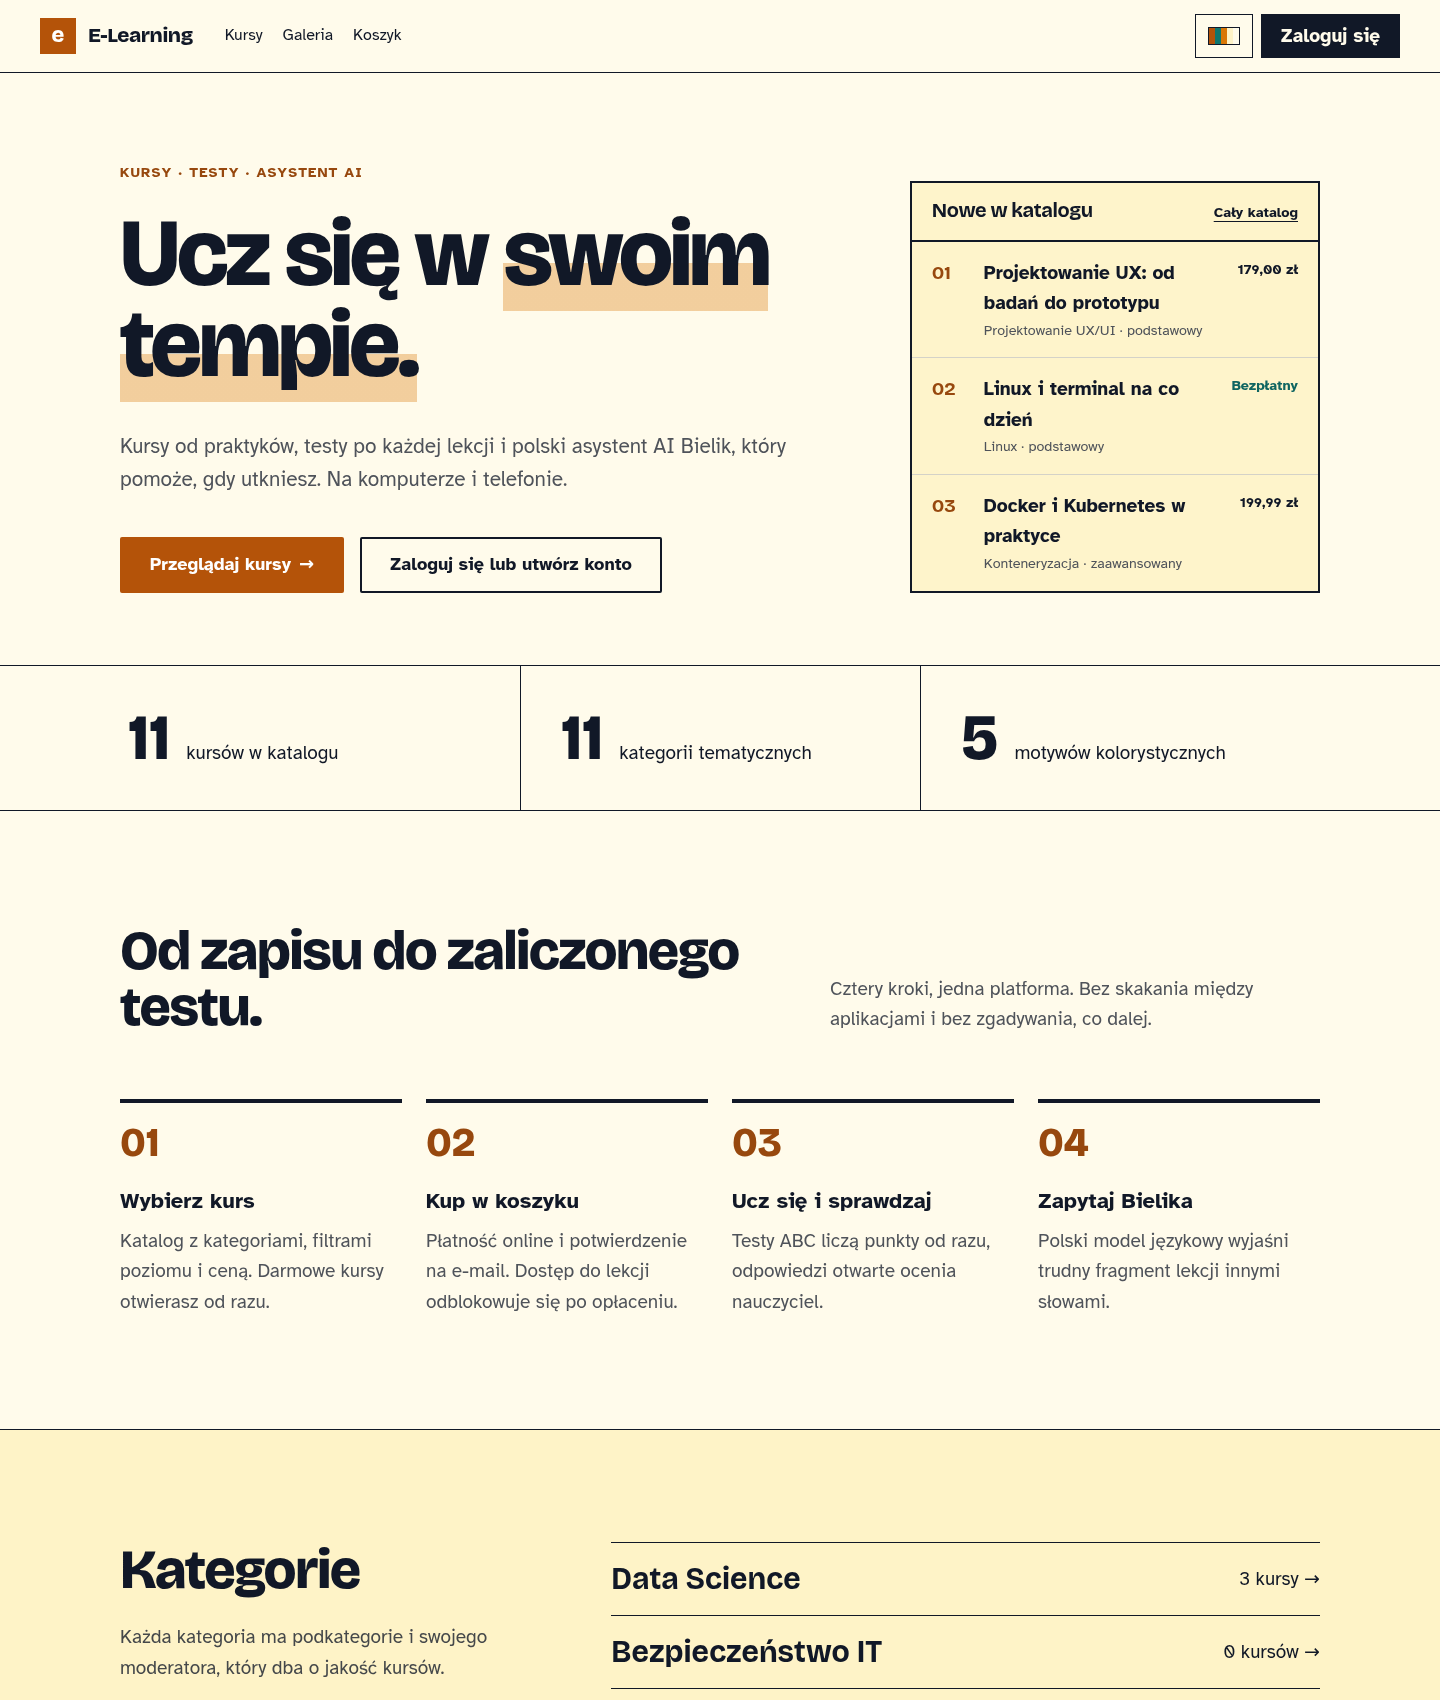
\includegraphics[width=0.94\linewidth,height=0.37\textheight,keepaspectratio]{img/home.png}}
\caption{Strona główna (gość, motyw domyślny ,,Bursztyn'')}\label{fig:ui-home}
\end{figure}
Nagłówek zawiera logo, menu główne, przełącznik motywu i~przycisk logowania. Pod sekcją powitalną widać najnowsze kursy z~bazy, prawdziwe liczby (kursy, kategorie, motywy), cztery numerowane kroki i~listę kategorii z~licznikami.


\begin{figure}[H]
\centering
\fcolorbox{rule}{white}{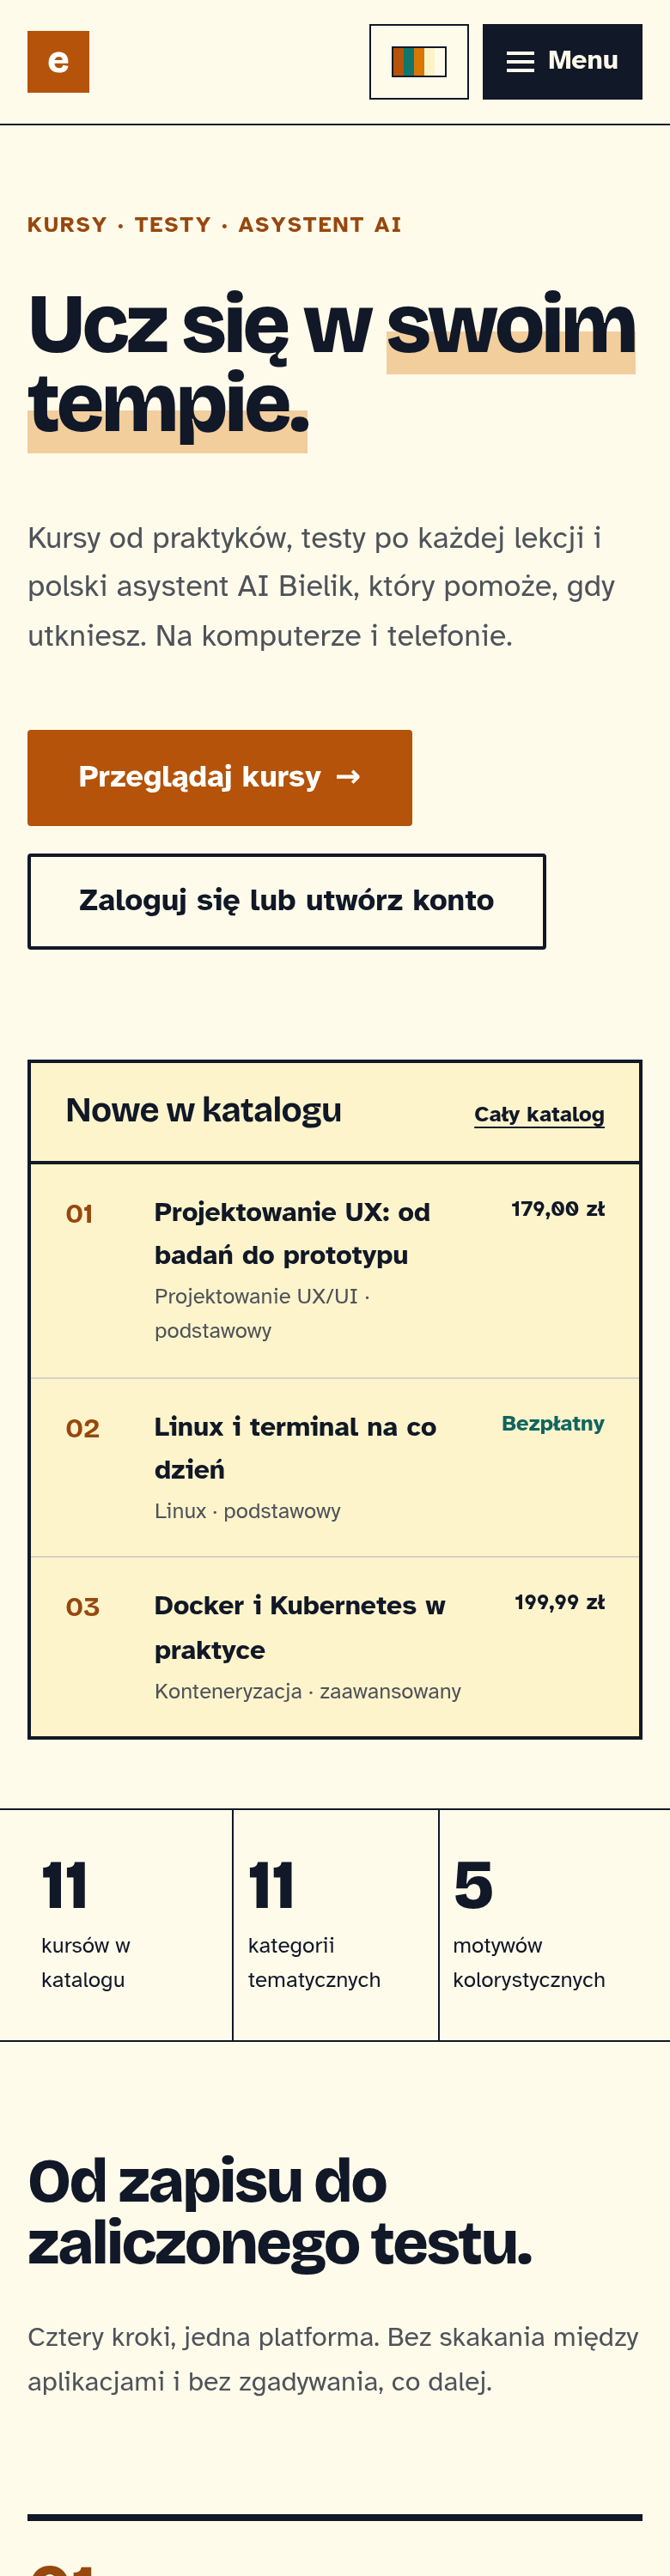
\includegraphics[width=0.94\linewidth,height=0.42\textheight,keepaspectratio]{img/home_mobile.png}}
\caption{Strona główna na telefonie (390 px)}\label{fig:ui-home-mobile}
\end{figure}
Menu zwija się do przycisku ,,Menu'', siatki przechodzą w~jedną kolumnę, nie pojawia się poziomy pasek przewijania.


\section{Konto}

\begin{figure}[H]
\centering
\fcolorbox{rule}{white}{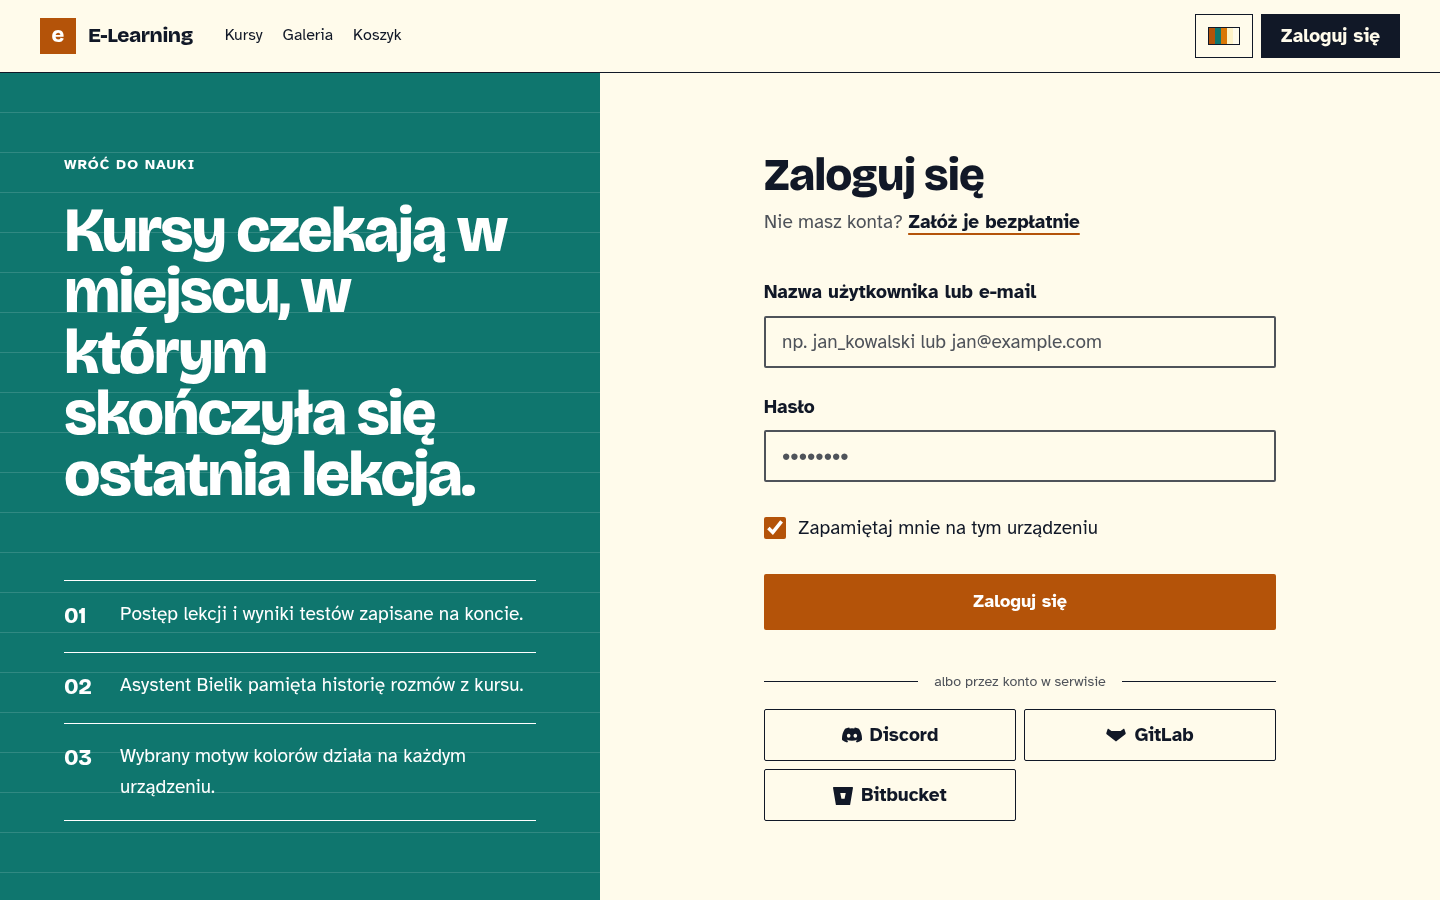
\includegraphics[width=0.94\linewidth,height=0.37\textheight,keepaspectratio]{img/login.png}}
\caption{Logowanie -- układ split-screen}\label{fig:ui-login}
\end{figure}
Na komputerze panel informacyjny stoi obok formularza (asymetrycznie), a~pod formularzem są przyciski portali Discord, GitLab i~Bitbucket. Każde pole ma etykietę, a~,,Zapamiętaj mnie'' to zwykłe pole wyboru.


\begin{figure}[H]
\centering
\fcolorbox{rule}{white}{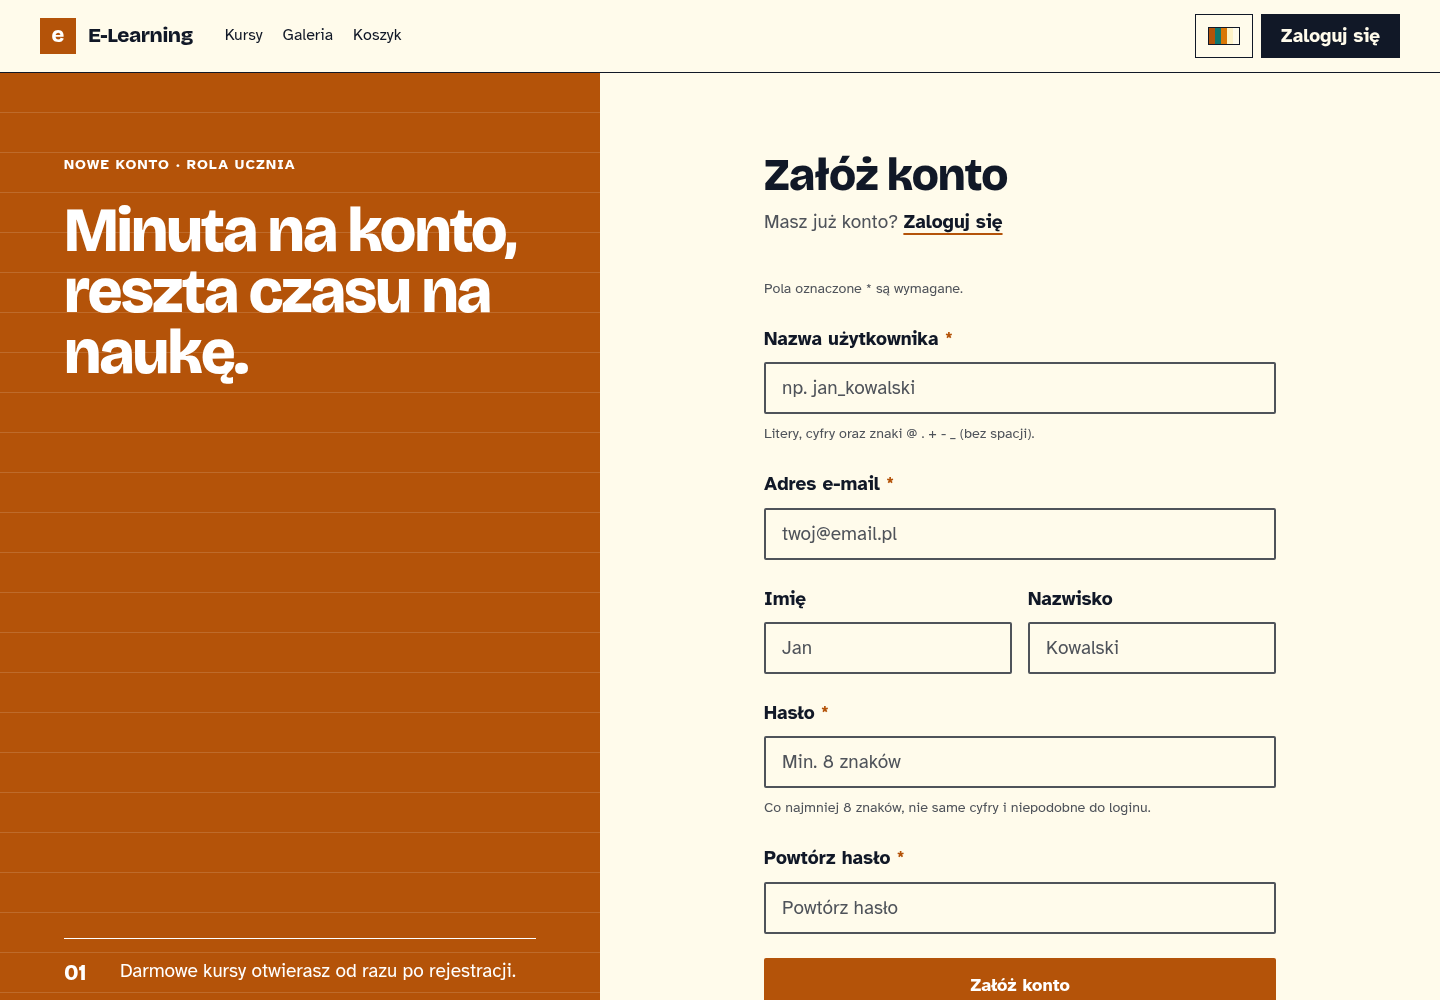
\includegraphics[width=0.94\linewidth,height=0.37\textheight,keepaspectratio]{img/register.png}}
\caption{Rejestracja}\label{fig:ui-register}
\end{figure}
Dostępność loginu i~e-maila jest sprawdzana podczas pisania; przy błędzie formularz zachowuje dane poza hasłami.


\begin{figure}[H]
\centering
\fcolorbox{rule}{white}{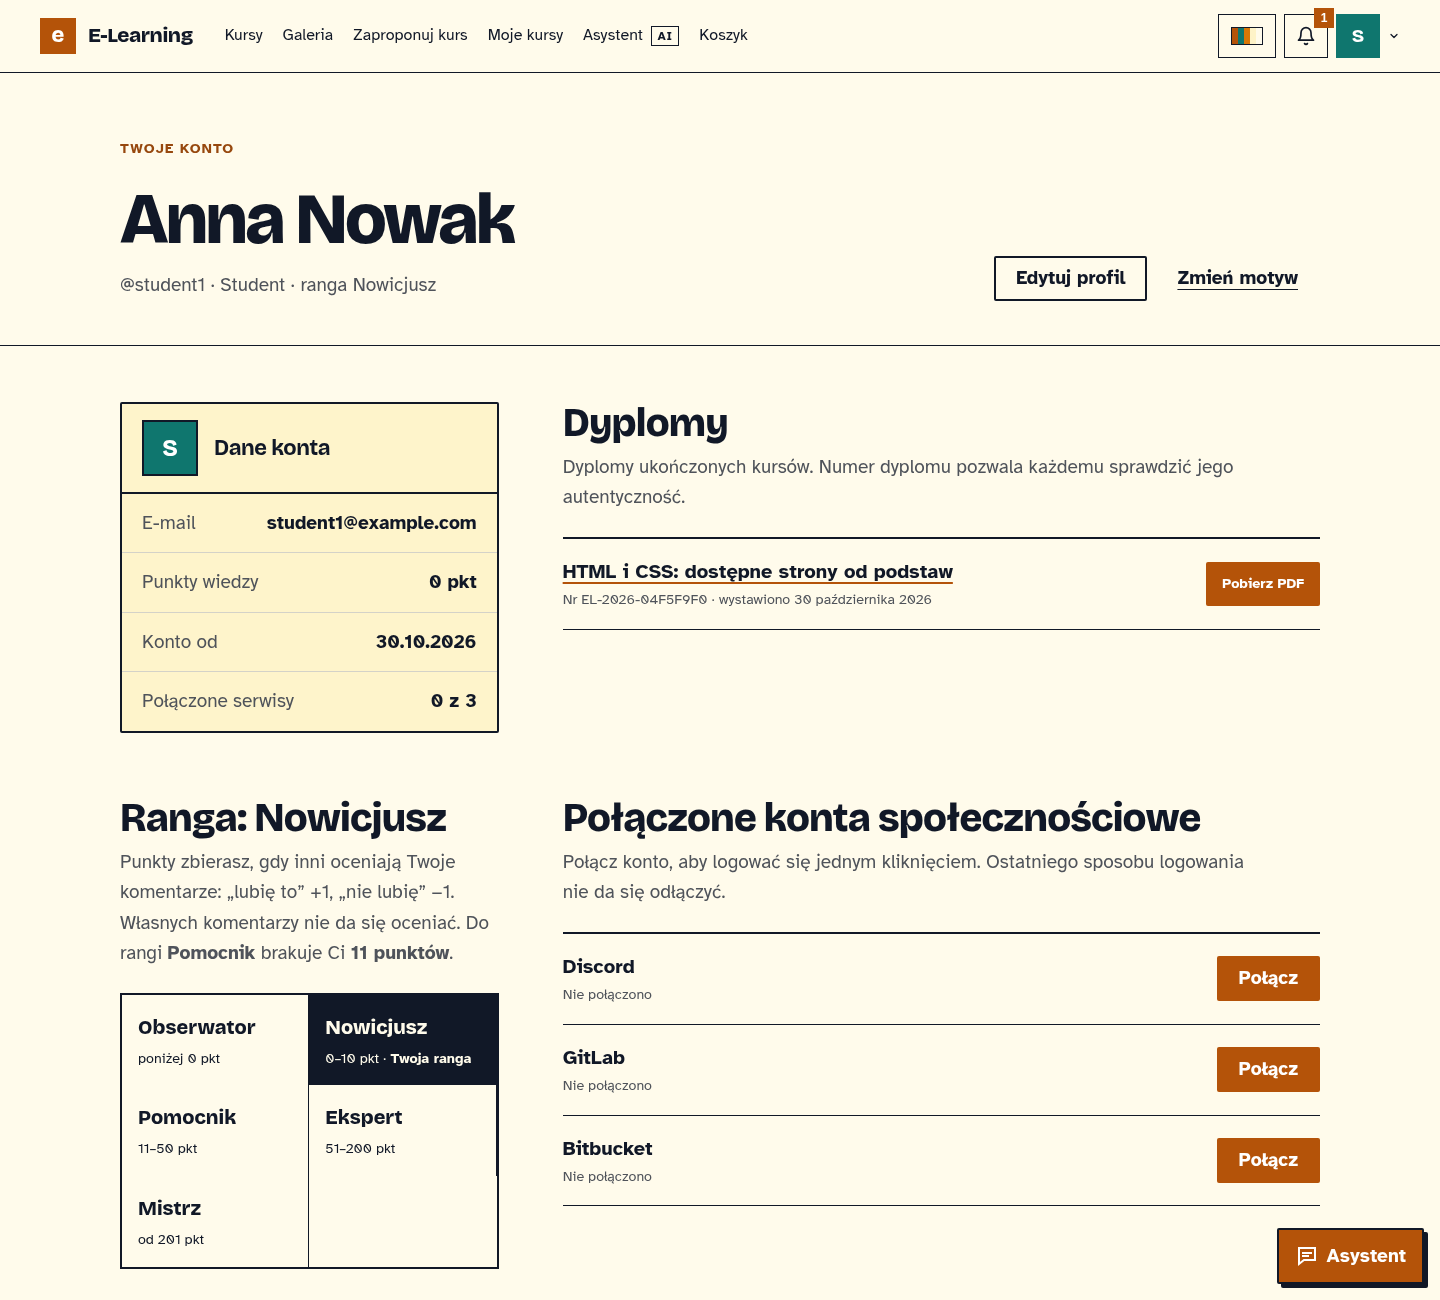
\includegraphics[width=0.94\linewidth,height=0.37\textheight,keepaspectratio]{img/profile.png}}
\caption{Profil ucznia}\label{fig:ui-profile}
\end{figure}
Dane konta, dyplomy do pobrania, ranga z~drabiną rang (ile punktów do następnej) i~połączone konta portali z~przyciskami łączenia/odłączania.


\begin{figure}[H]
\centering
\fcolorbox{rule}{white}{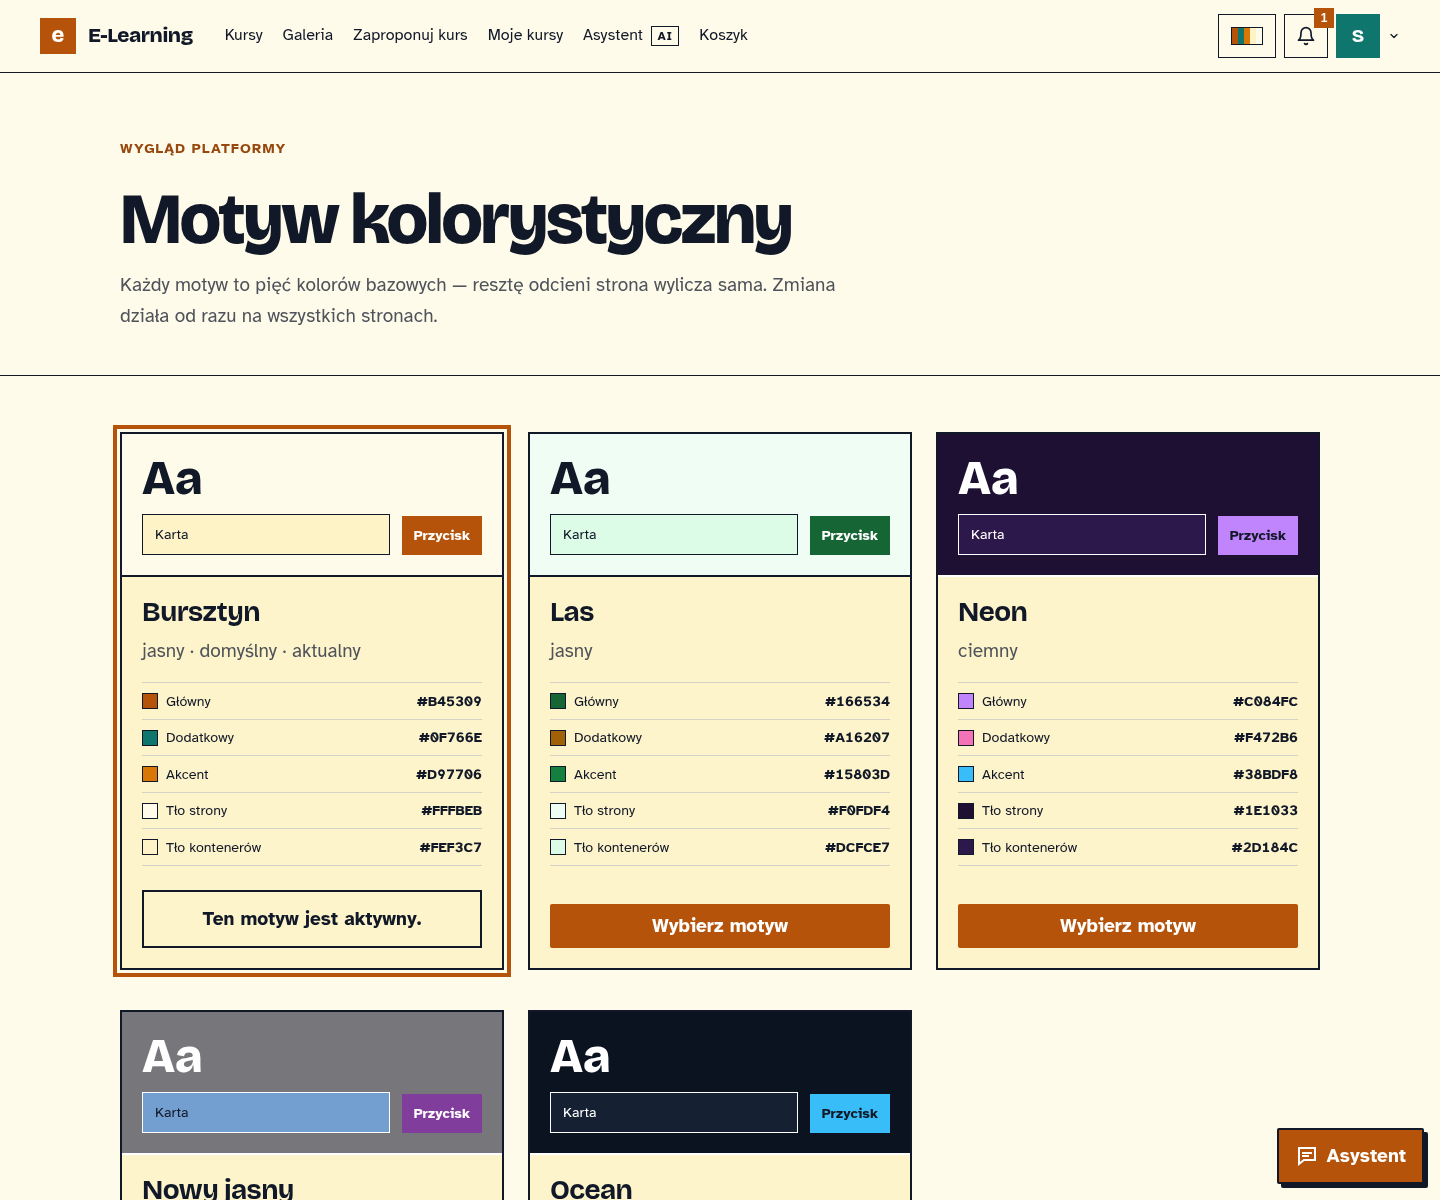
\includegraphics[width=0.94\linewidth,height=0.37\textheight,keepaspectratio]{img/themes.png}}
\caption{Wybór motywu}\label{fig:ui-themes}
\end{figure}
Każdy motyw jest pokazany na próbce interfejsu; wybór zapisuje się w~profilu.


\section{Katalog i~kurs}

\begin{figure}[H]
\centering
\fcolorbox{rule}{white}{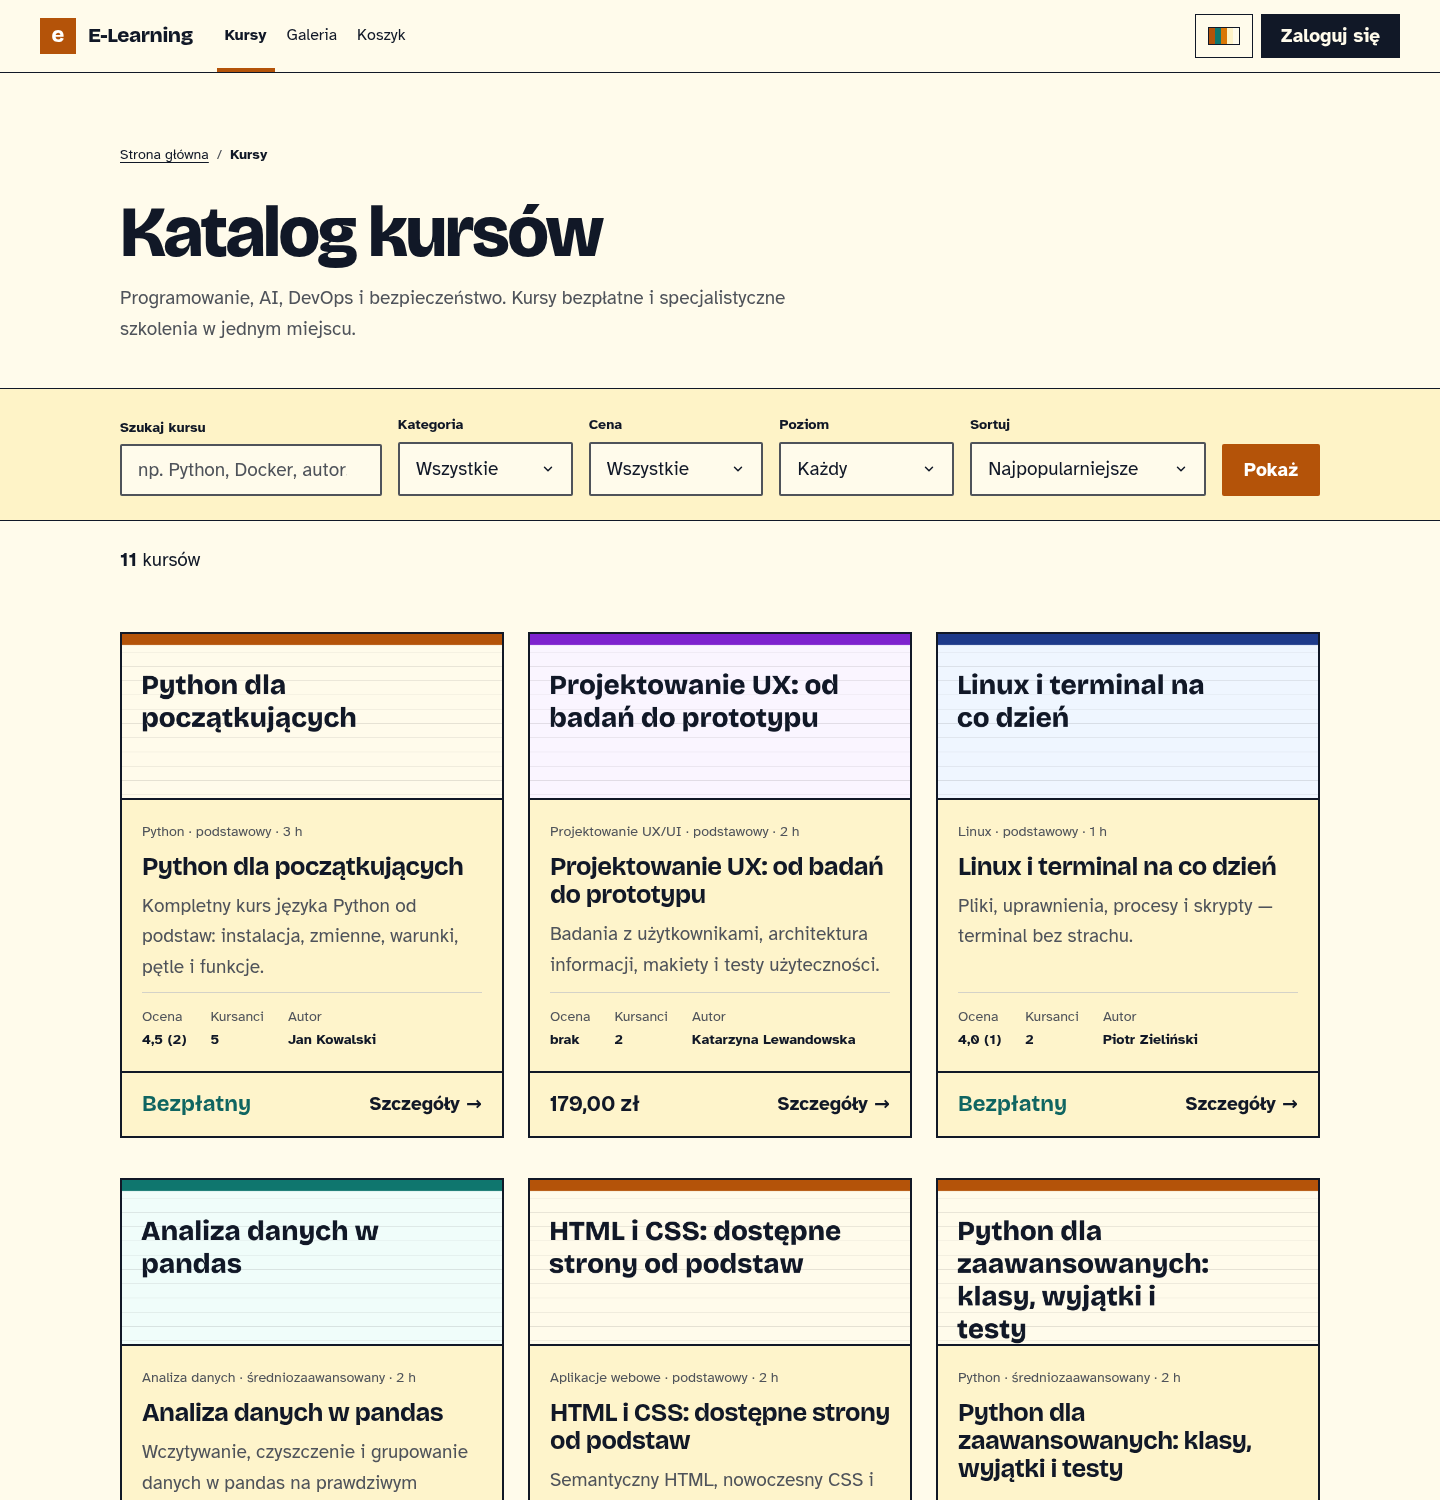
\includegraphics[width=0.94\linewidth,height=0.37\textheight,keepaspectratio]{img/catalog.png}}
\caption{Katalog kursów}\label{fig:ui-catalog}
\end{figure}
Wyszukiwarka i~filtry (kategoria, poziom, cena, sortowanie) w~jednym pasku, siatka kart w~trzech kolumnach, paginacja.


\begin{figure}[H]
\centering
\fcolorbox{rule}{white}{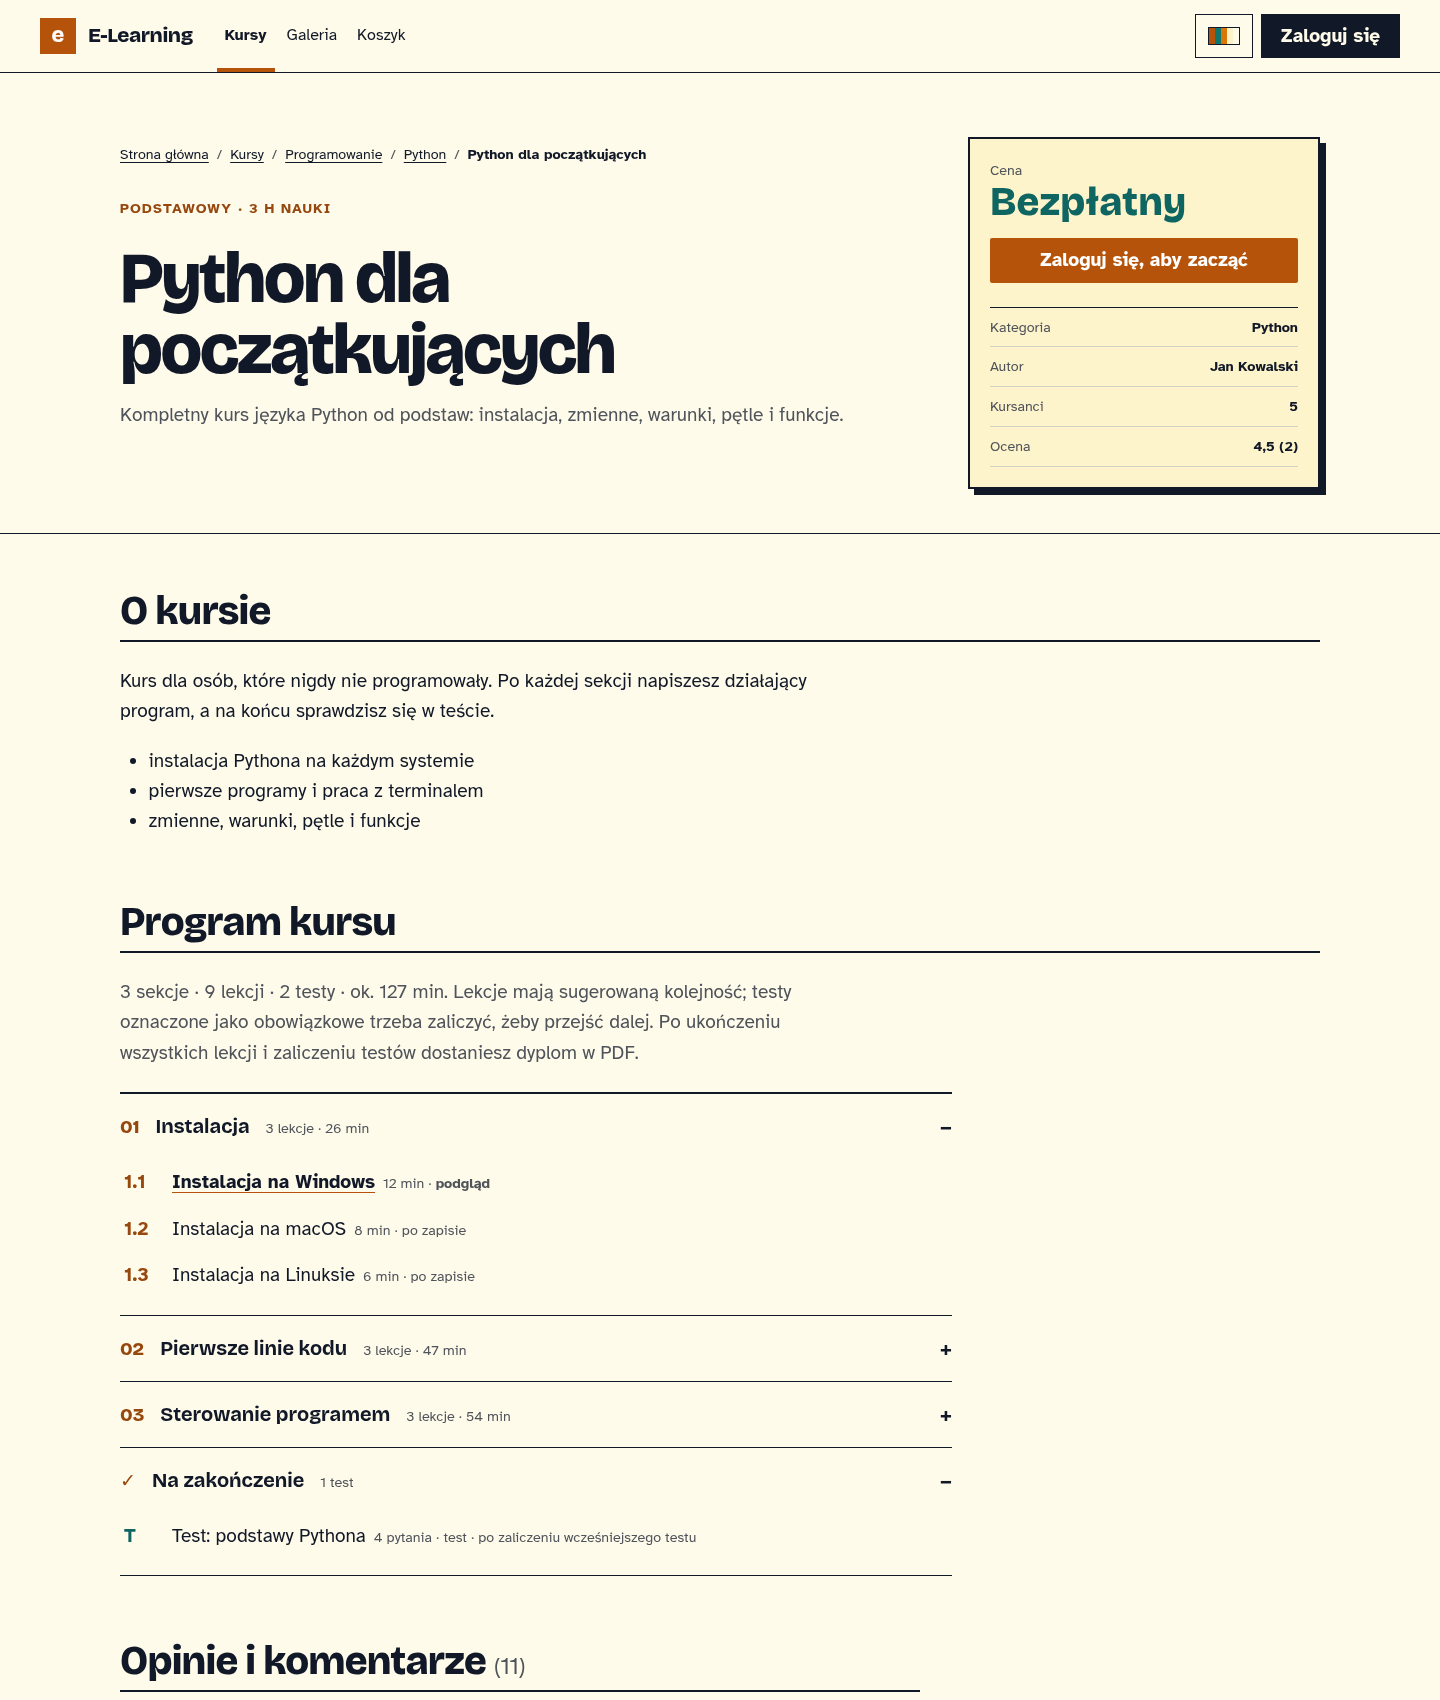
\includegraphics[width=0.94\linewidth,height=0.37\textheight,keepaspectratio]{img/course.png}}
\caption{Strona kursu}\label{fig:ui-course}
\end{figure}
Okruszki, opis ,,O kursie'', program z~czasem trwania, panel zakupu z~ceną lub przyciskiem zapisu oraz komentarze w~wątkach.


\section{Nauka}

\begin{figure}[H]
\centering
\fcolorbox{rule}{white}{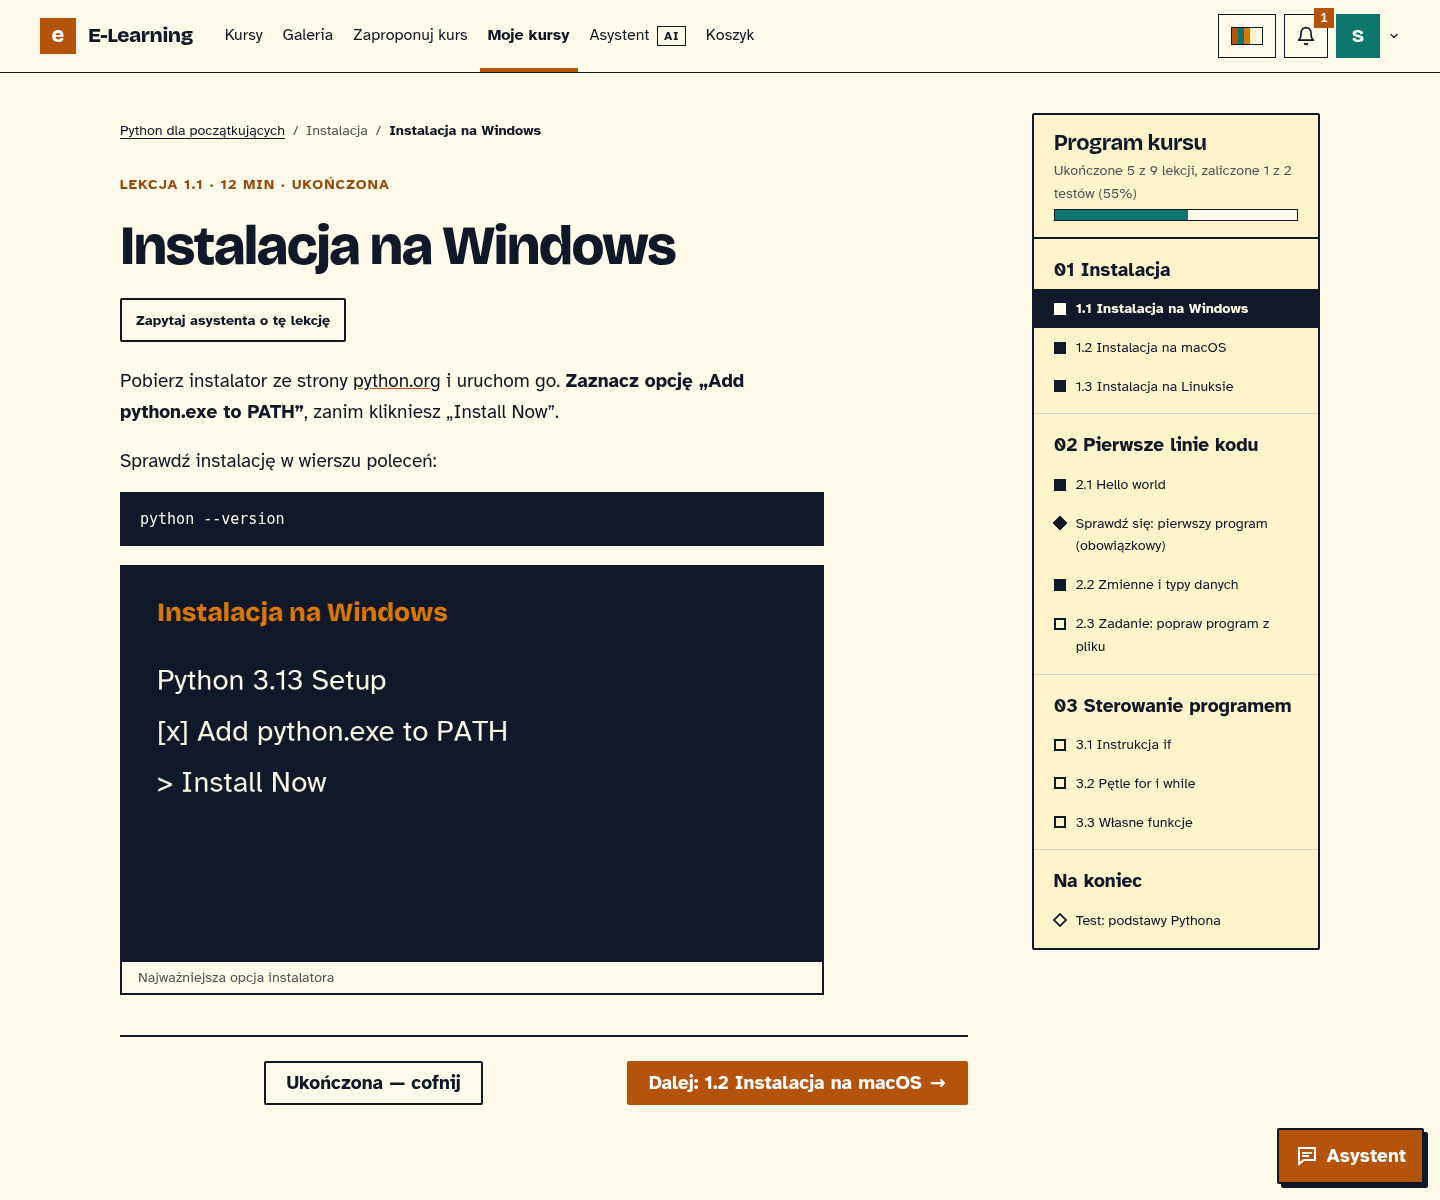
\includegraphics[width=0.94\linewidth,height=0.37\textheight,keepaspectratio]{img/lesson.png}}
\caption{Lekcja z~programem kursu}\label{fig:ui-lesson}
\end{figure}
Po lewej treść lekcji (kod, zdjęcie z~podpisem), po prawej program z~postępem i~oznaczeniami: ukończona (pełny kwadrat), test (romb), test obowiązkowy. Przycisk ,,Zapytaj asystenta o~tę lekcję'' otwiera czat z~kontekstem.


\begin{figure}[H]
\centering
\fcolorbox{rule}{white}{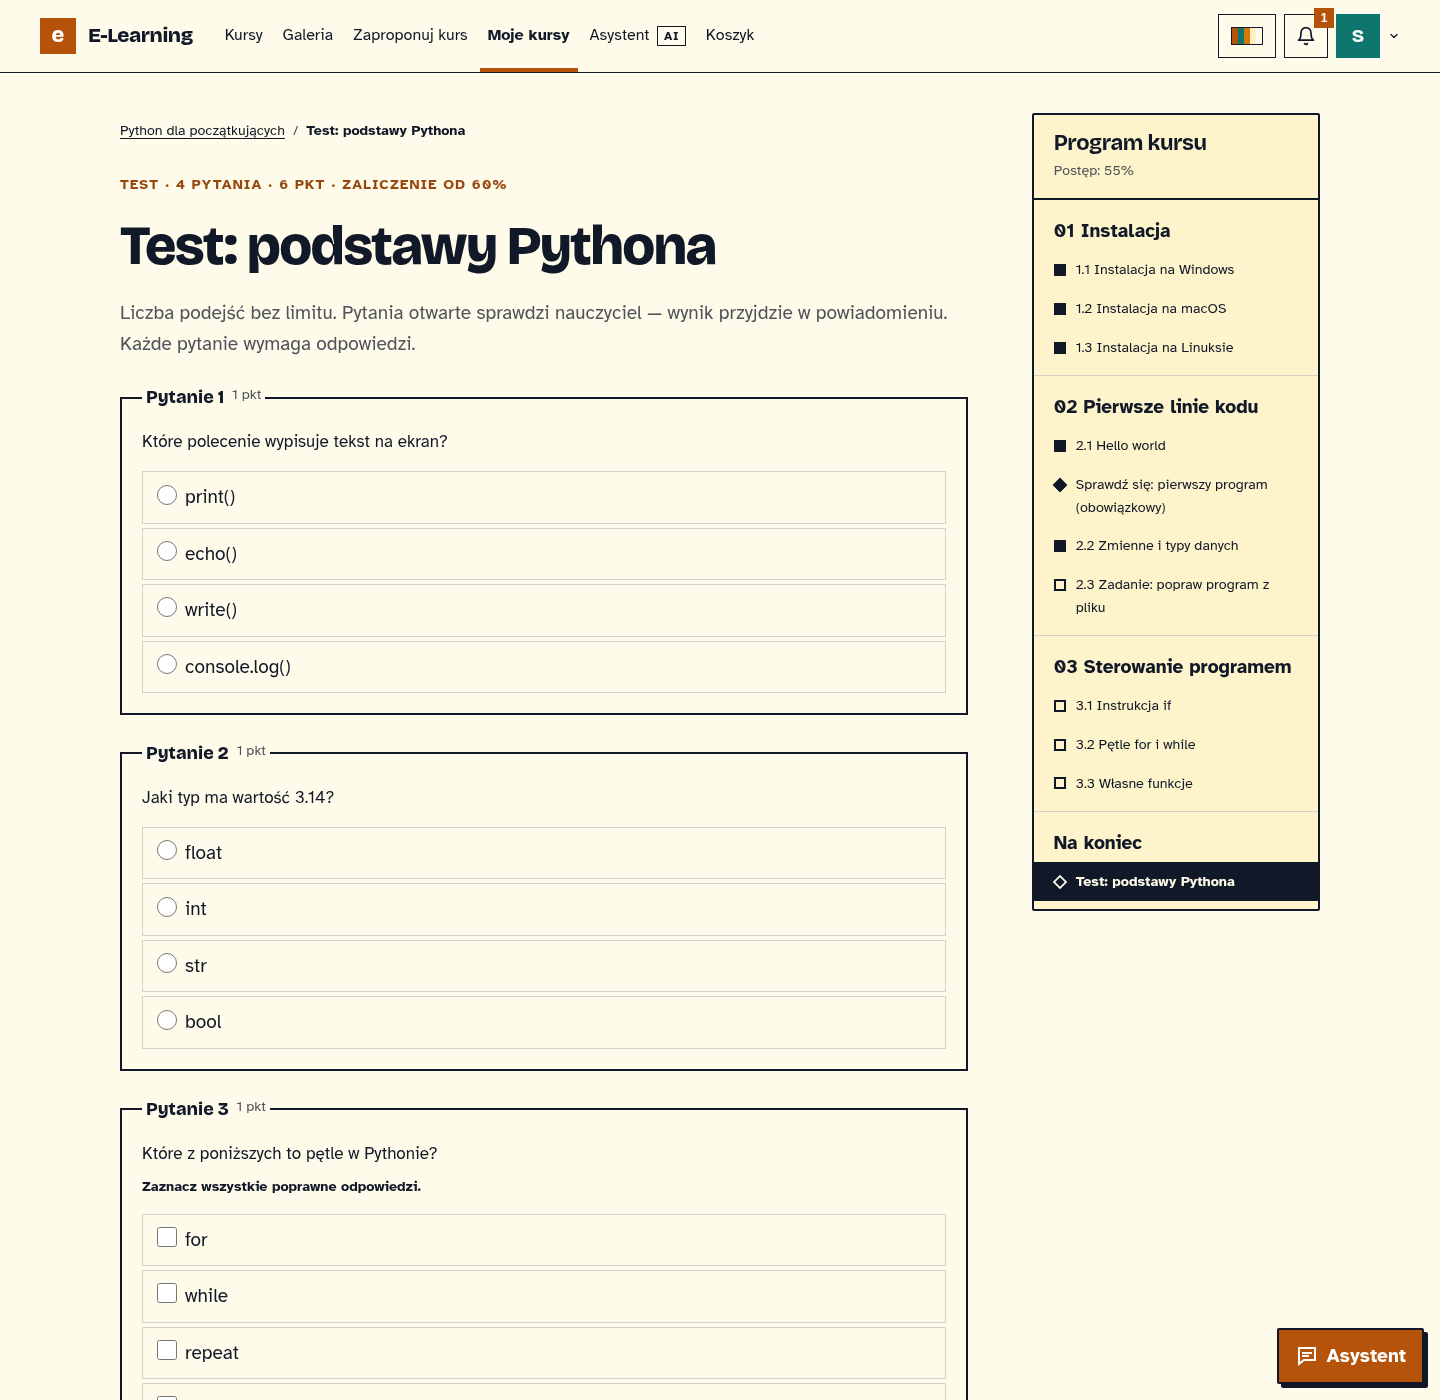
\includegraphics[width=0.94\linewidth,height=0.37\textheight,keepaspectratio]{img/quiz.png}}
\caption{Rozwiązywanie testu}\label{fig:ui-quiz}
\end{figure}
Każde pytanie to \code{fieldset} z~\code{legend} (numer i~punkty); odpowiedzi jednokrotnego wyboru jako pola radio, wielokrotnego -- pola wyboru z~instrukcją ,,Zaznacz wszystkie poprawne odpowiedzi''.


\begin{figure}[H]
\centering
\fcolorbox{rule}{white}{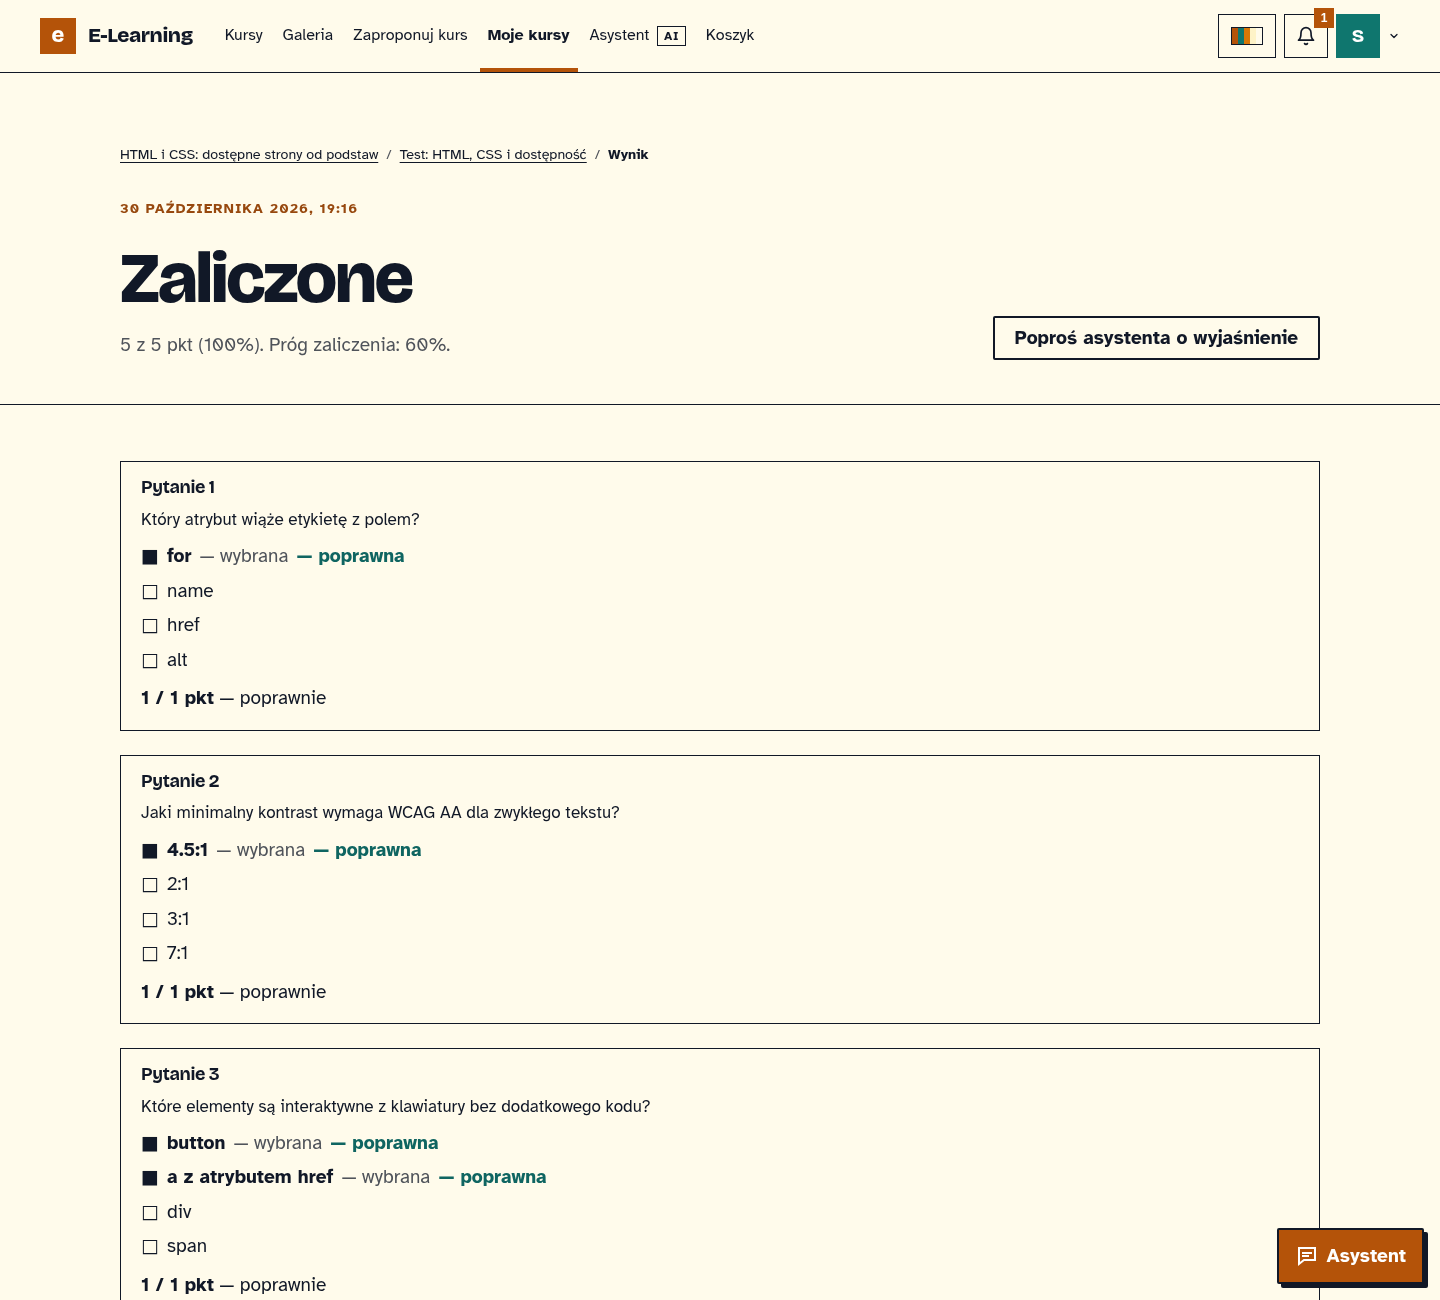
\includegraphics[width=0.94\linewidth,height=0.37\textheight,keepaspectratio]{img/attempt.png}}
\caption{Wynik testu}\label{fig:ui-attempt}
\end{figure}
Wynik procentowy, punkty za każde pytanie, poprawne odpowiedzi (po zaliczeniu) i~przycisk ,,Poproś asystenta o~wyjaśnienie''.


\begin{figure}[H]
\centering
\fcolorbox{rule}{white}{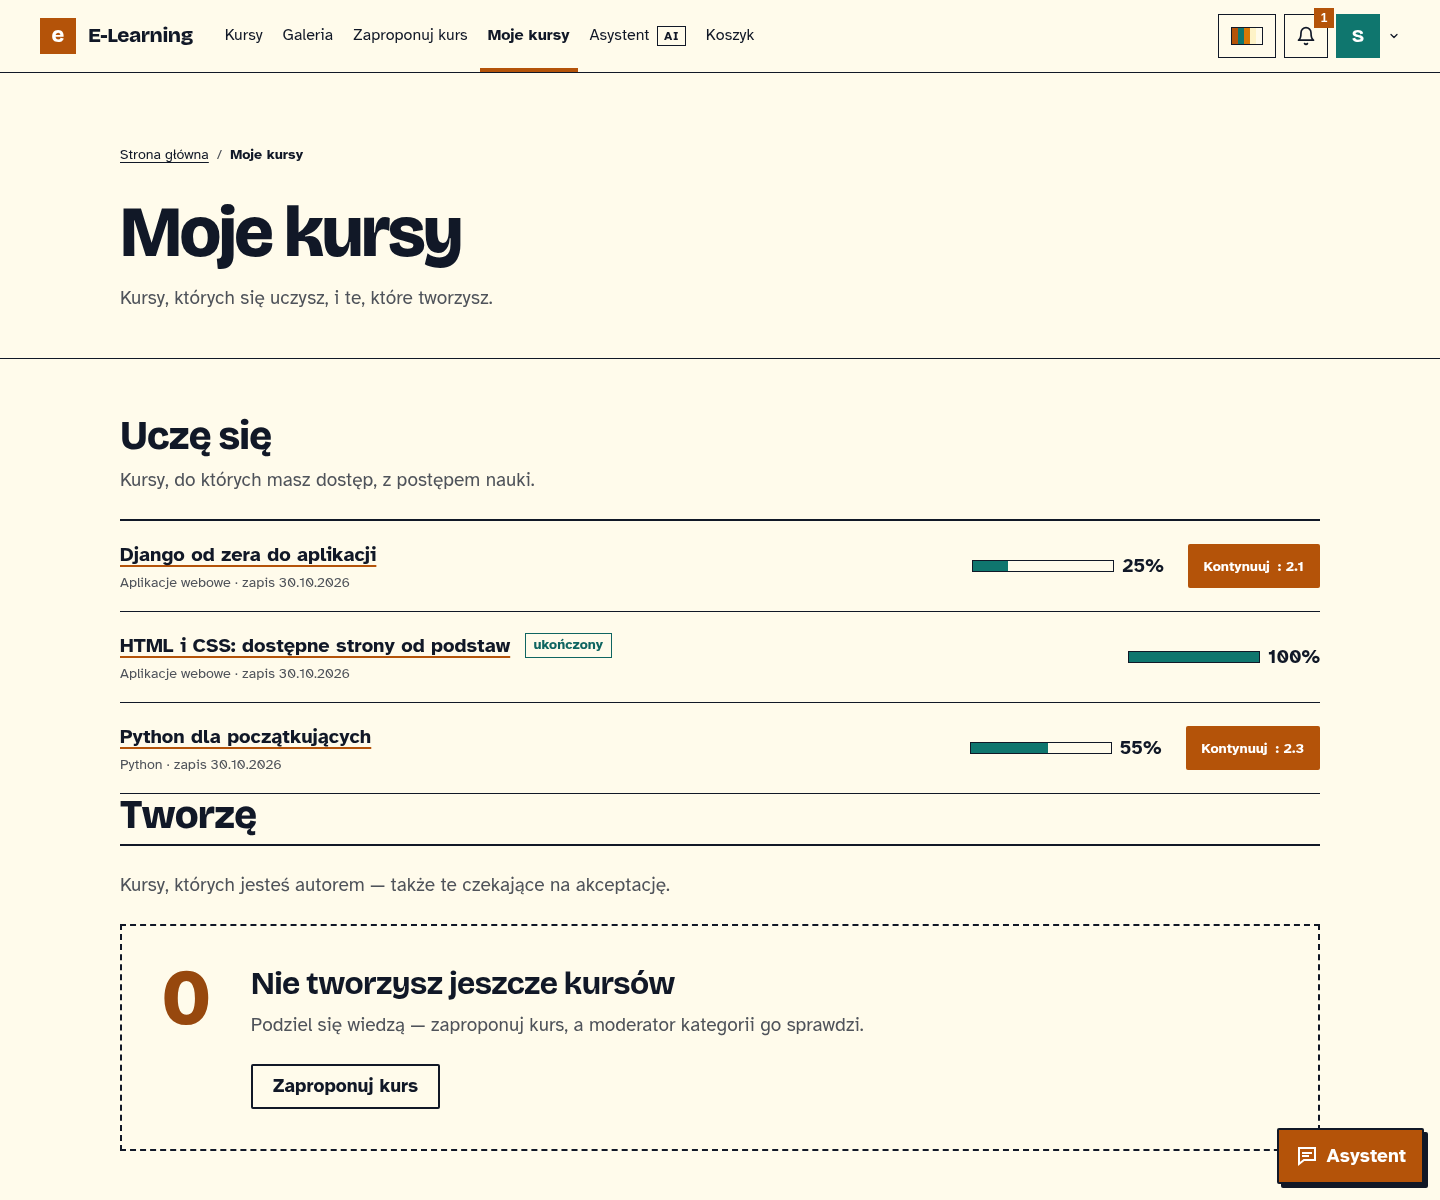
\includegraphics[width=0.94\linewidth,height=0.37\textheight,keepaspectratio]{img/mycourses.png}}
\caption{Moje kursy}\label{fig:ui-mycourses}
\end{figure}
Zakładka ,,Uczę się'' z~paskami postępu i~,,Tworzę'' ze stanem zgłoszeń; pusta sekcja pokazuje stan pusty z~zachętą.


\section{Asystent AI}

\begin{figure}[H]
\centering
\fcolorbox{rule}{white}{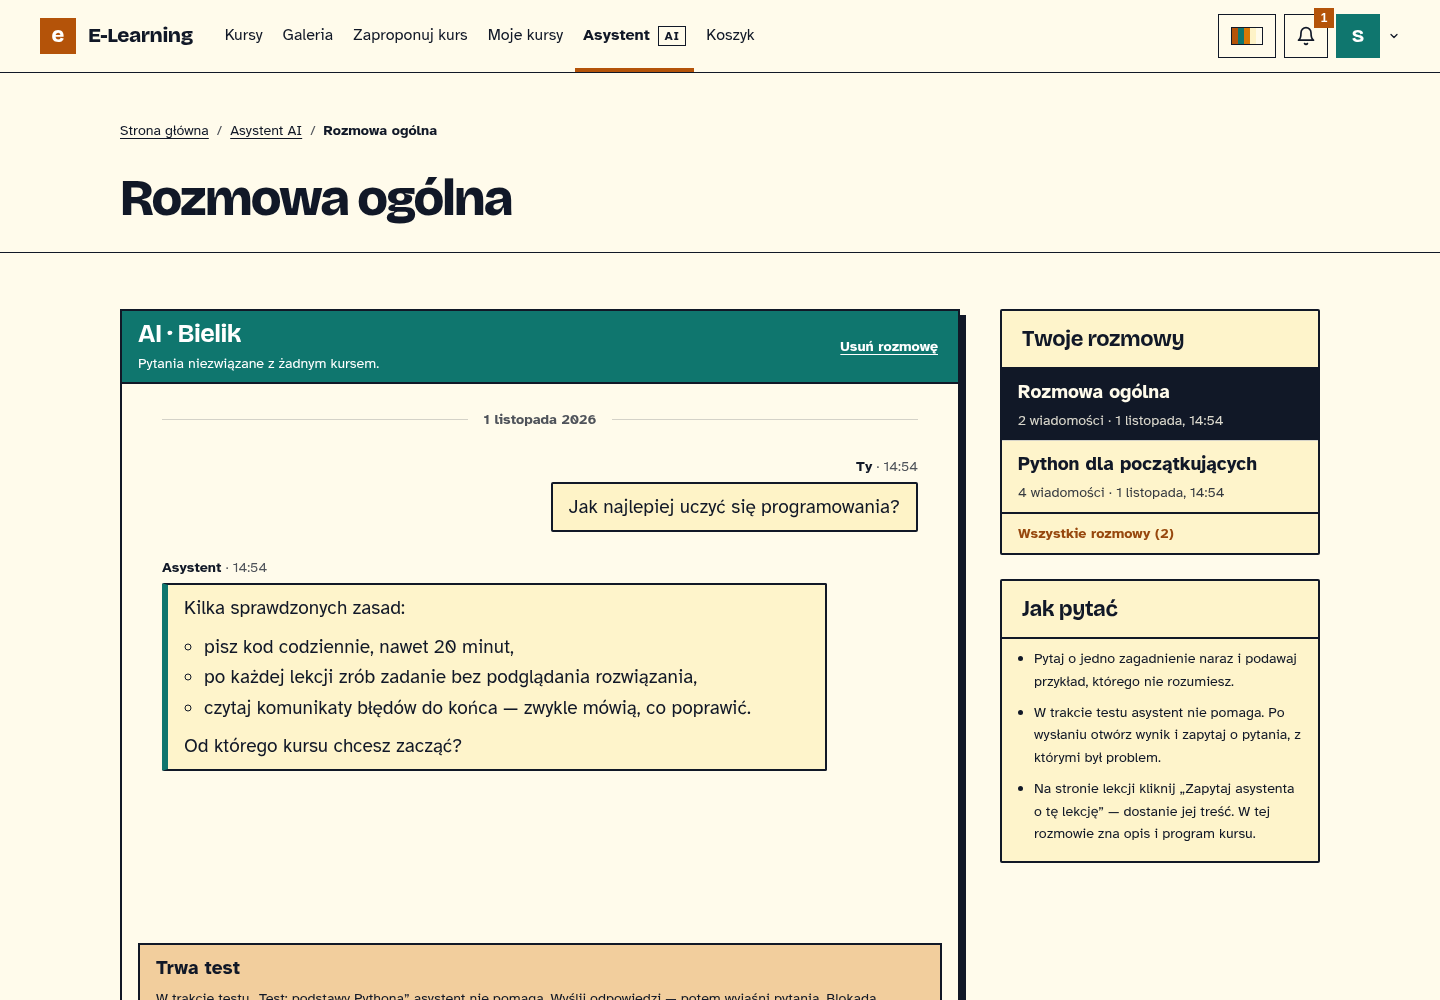
\includegraphics[width=0.94\linewidth,height=0.37\textheight,keepaspectratio]{img/chat.png}}
\caption{Strona rozmowy z~asystentem}\label{fig:ui-chat}
\end{figure}
Ramka czatu z~historią i~boczną listą rozmów (ogólna i~po jednej na kurs). Odpowiedzi są formatowane (listy, pogrubienia, kod).


\section{Sklep}

\begin{figure}[H]
\centering
\fcolorbox{rule}{white}{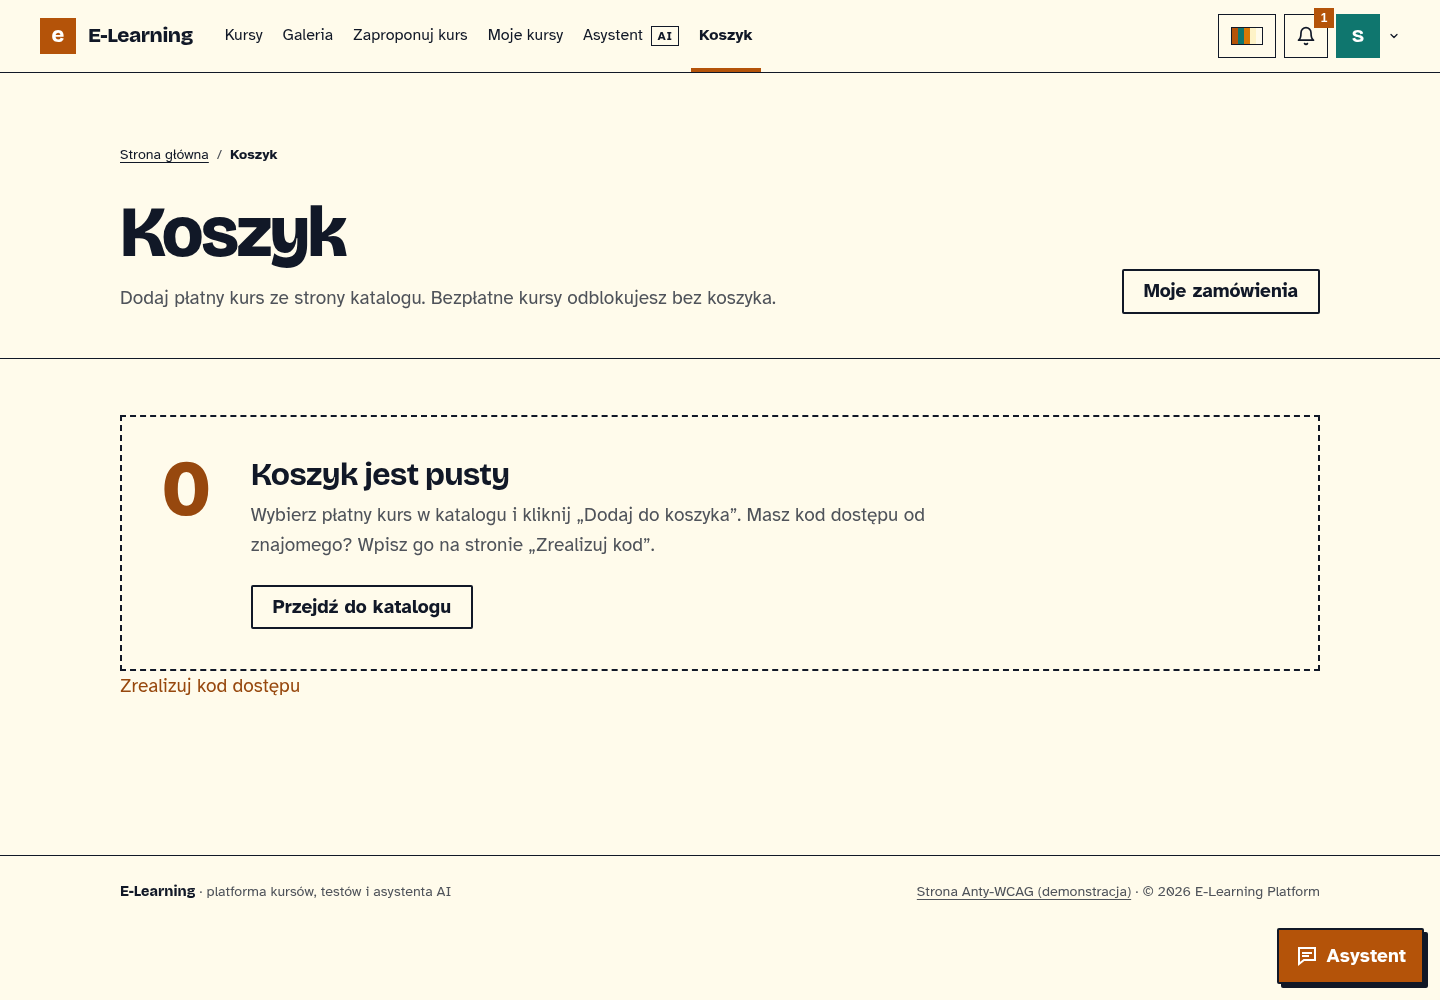
\includegraphics[width=0.94\linewidth,height=0.37\textheight,keepaspectratio]{img/cart.png}}
\caption{Koszyk -- stan pusty}\label{fig:ui-cart}
\end{figure}
Pusta lista nigdy nie jest pustą tabelą: komponent stanu pustego wyjaśnia sytuację i~proponuje następną akcję.


\begin{figure}[H]
\centering
\fcolorbox{rule}{white}{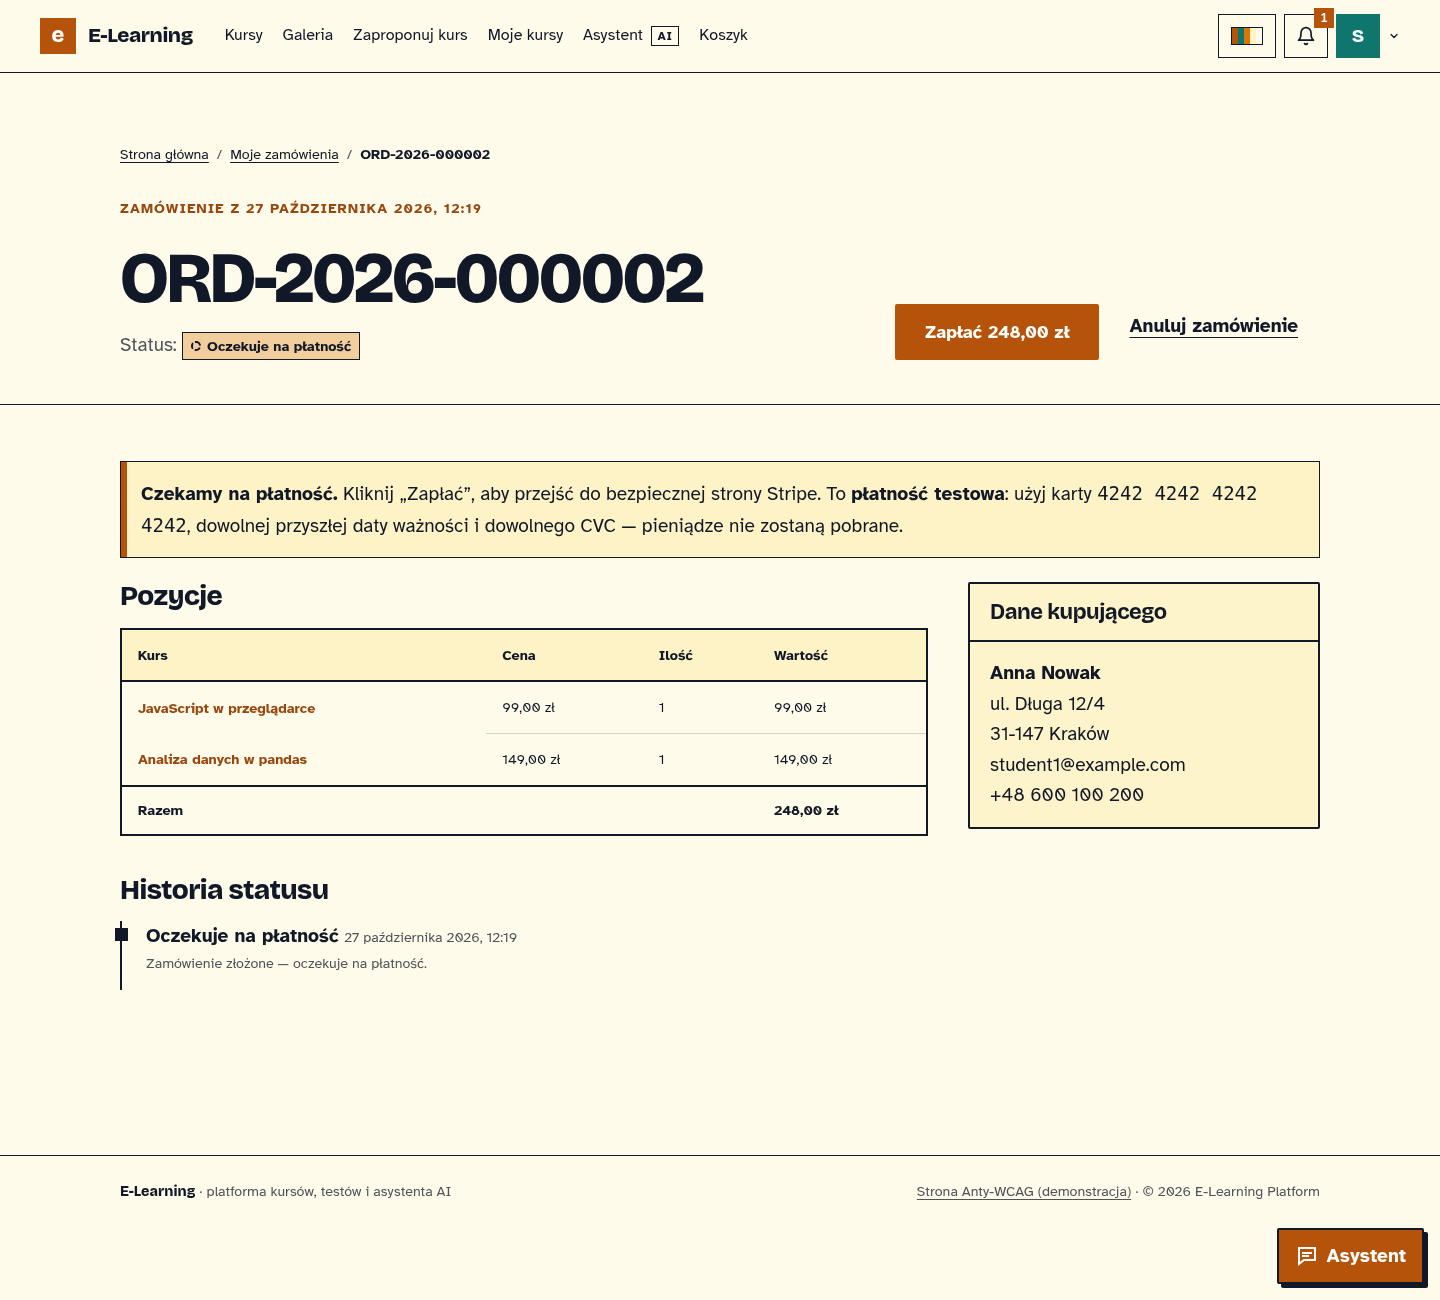
\includegraphics[width=0.94\linewidth,height=0.37\textheight,keepaspectratio]{img/order.png}}
\caption{Szczegóły zamówienia}\label{fig:ui-order}
\end{figure}
Numer, status, pozycje z~kodami dostępu, dane kupującego i~historia statusów; dla nieopłaconego zamówienia -- przycisk ,,Zapłać'' prowadzący do Stripe.


\section{Moderacja i~zarządzanie}

\begin{figure}[H]
\centering
\fcolorbox{rule}{white}{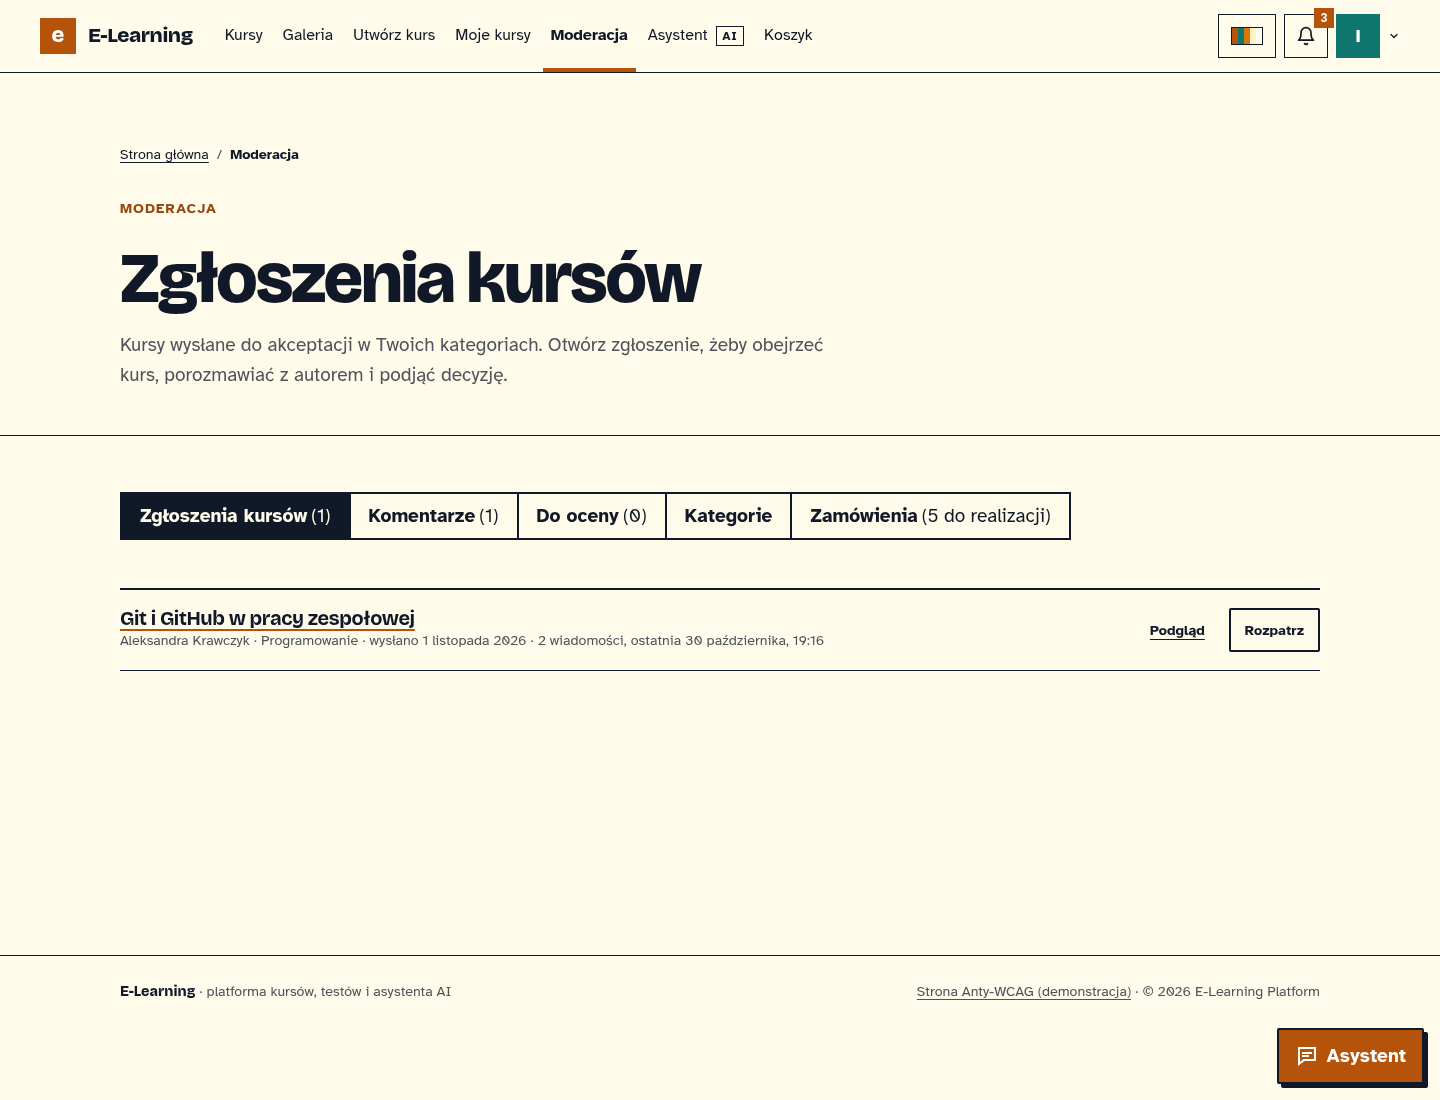
\includegraphics[width=0.94\linewidth,height=0.37\textheight,keepaspectratio]{img/moderation.png}}
\caption{Moderacja -- zgłoszenia kursów}\label{fig:ui-moderation}
\end{figure}
Zakładki: Zgłoszenia, Komentarze, Do oceny, Kategorie, Zamówienia -- z~licznikami oczekujących pozycji.


\begin{figure}[H]
\centering
\fcolorbox{rule}{white}{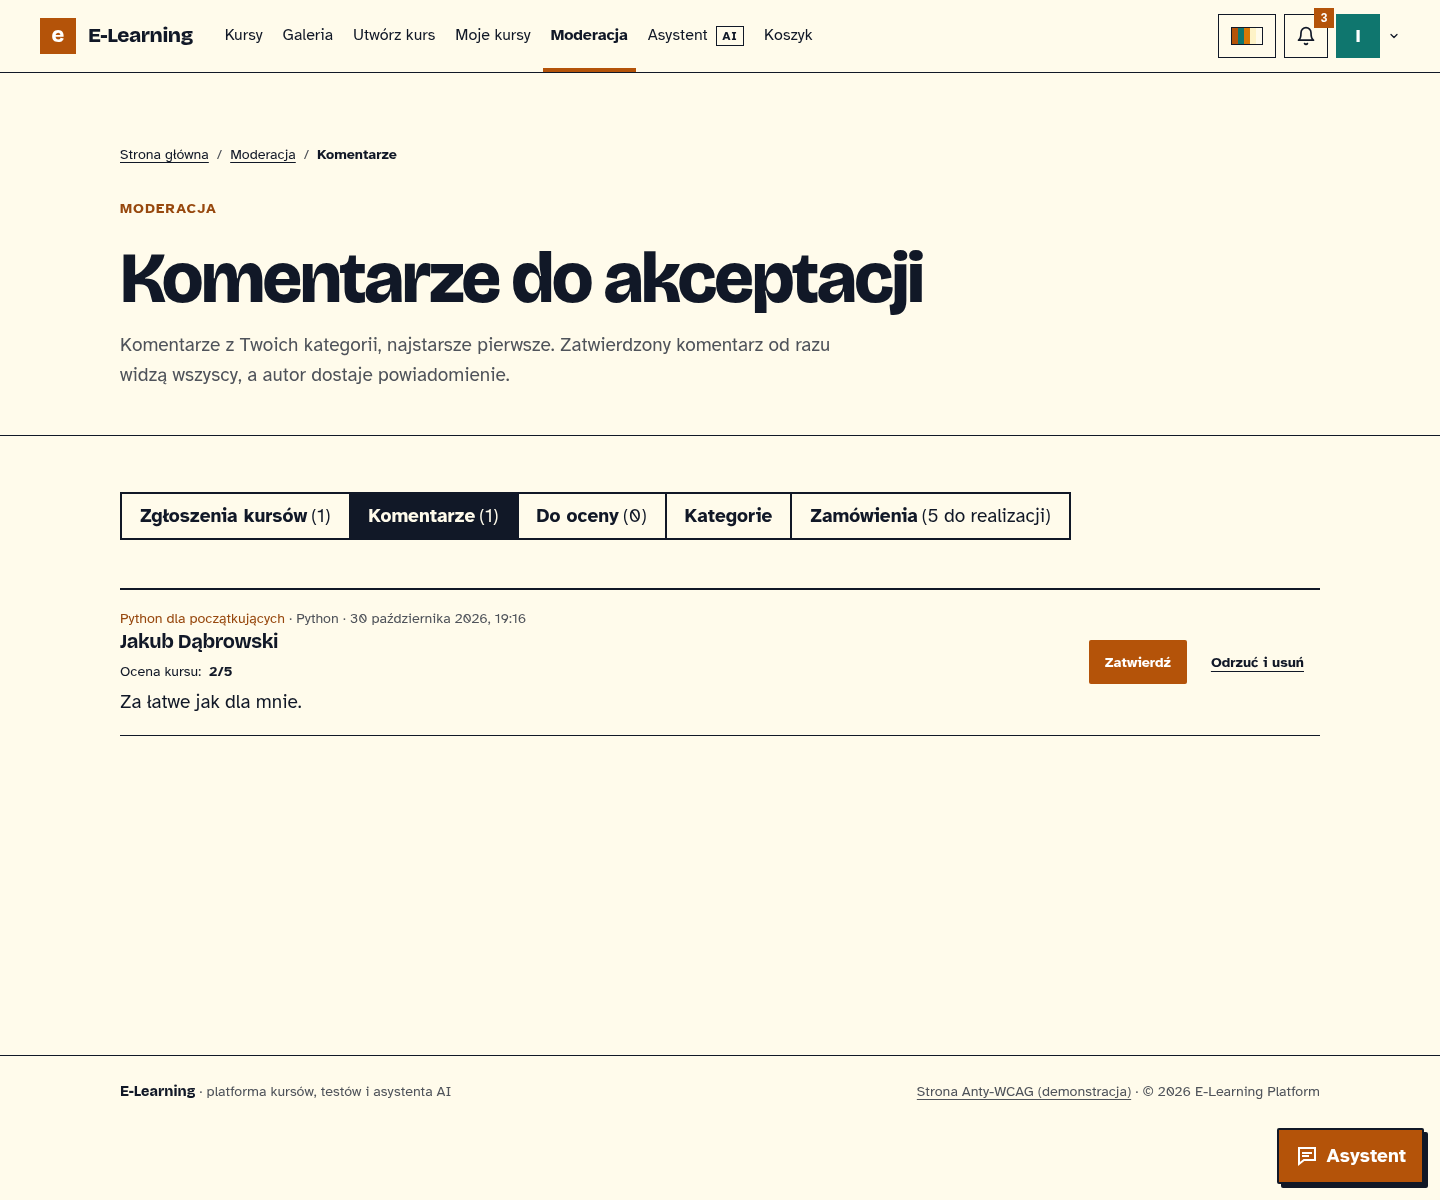
\includegraphics[width=0.94\linewidth,height=0.37\textheight,keepaspectratio]{img/mod_comments.png}}
\caption{Moderacja -- komentarze do akceptacji}\label{fig:ui-mod-comments}
\end{figure}
Akceptacja jednym kliknięciem, usunięcie z~dialogiem potwierdzenia.


\begin{figure}[H]
\centering
\fcolorbox{rule}{white}{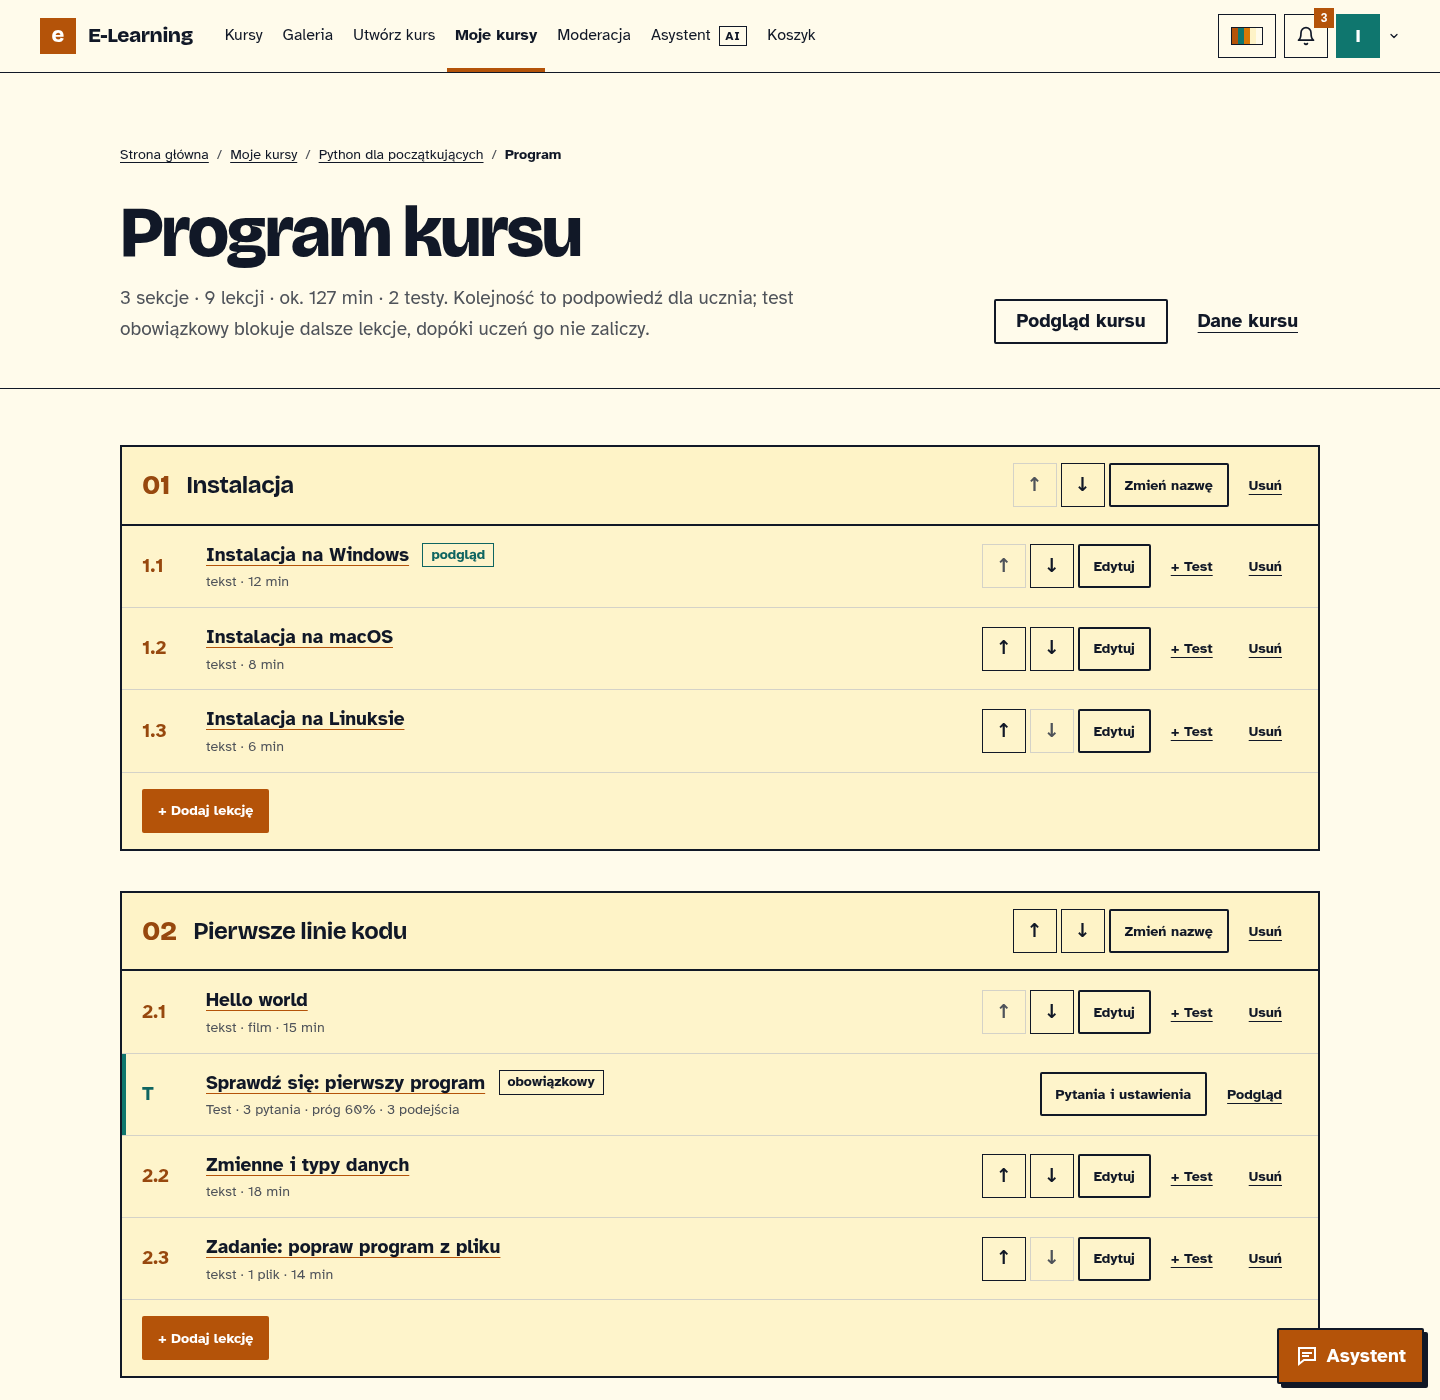
\includegraphics[width=0.94\linewidth,height=0.37\textheight,keepaspectratio]{img/curriculum.png}}
\caption{Kreator kursu -- krok 2: program}\label{fig:ui-curriculum}
\end{figure}
Sekcje i~lekcje z~przyciskami $\uparrow\downarrow$, edycją i~usuwaniem; testy wstawiane po lekcji lub na końcu.


\begin{figure}[H]
\centering
\fcolorbox{rule}{white}{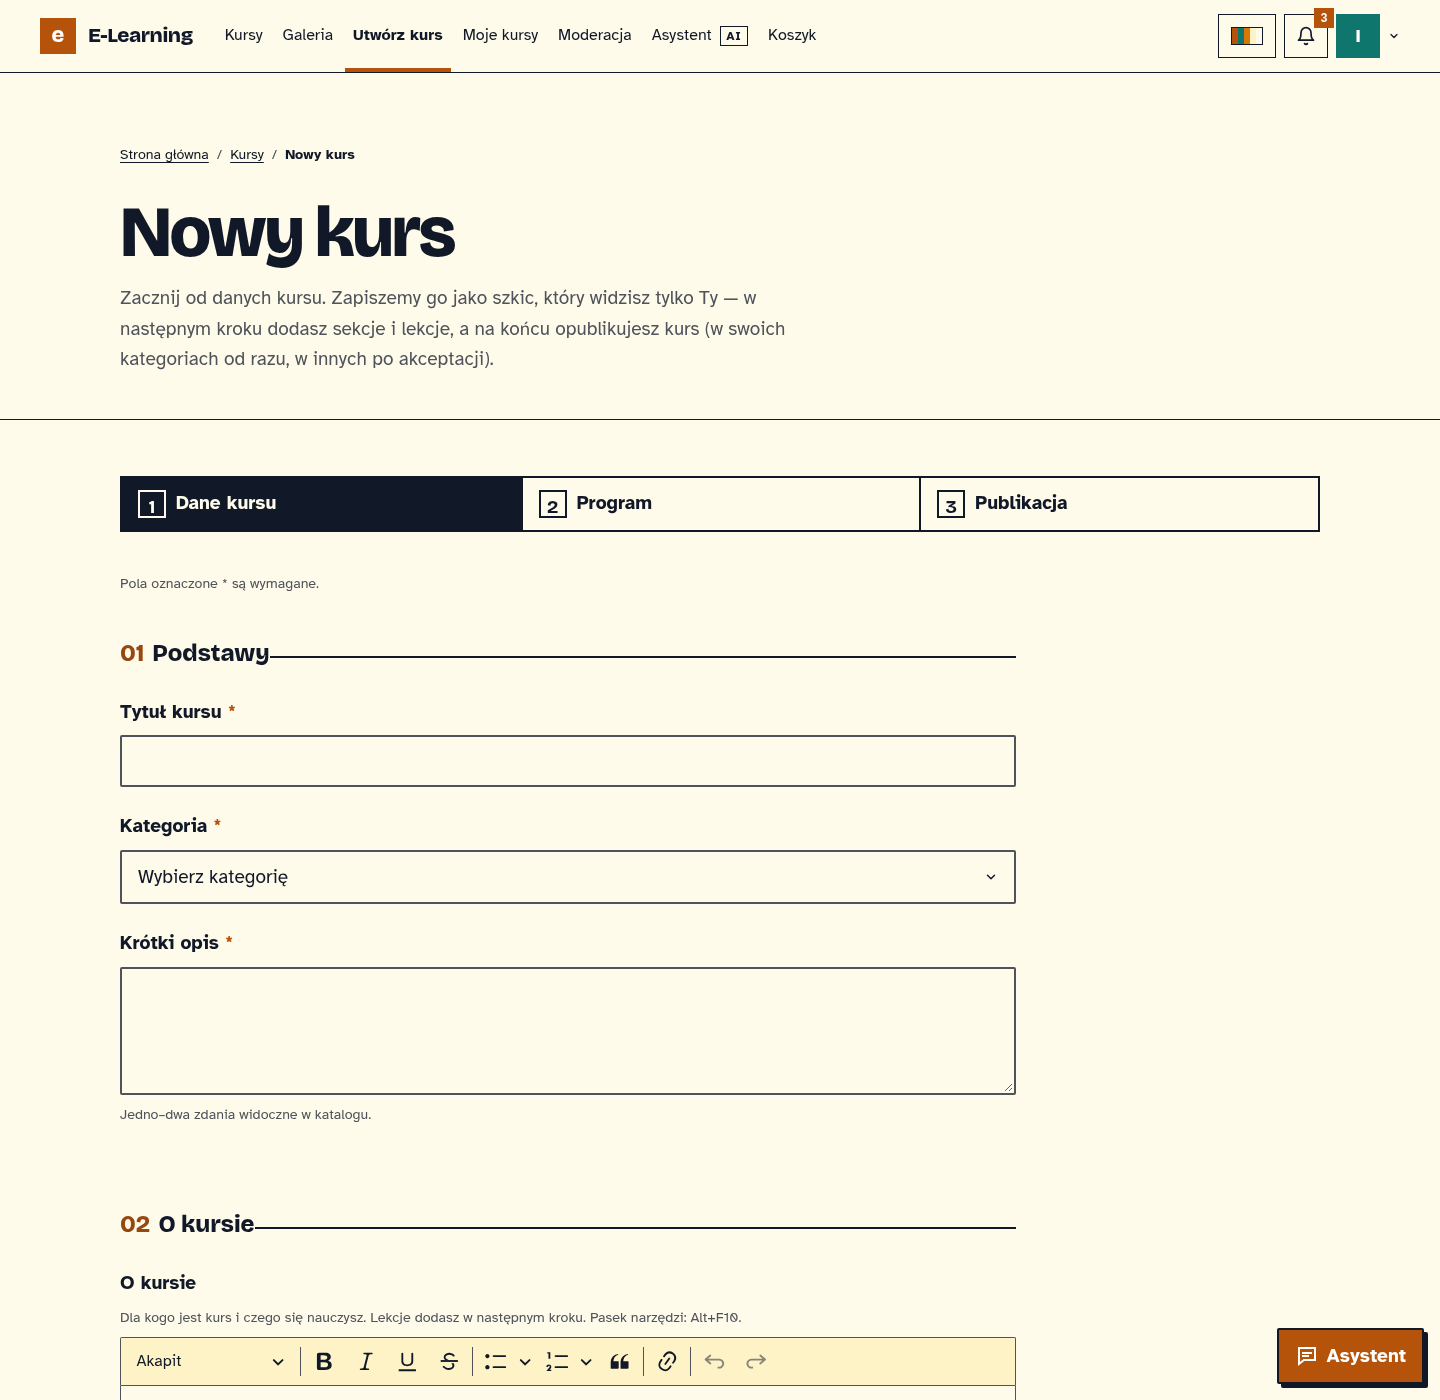
\includegraphics[width=0.94\linewidth,height=0.37\textheight,keepaspectratio]{img/course_create.png}}
\caption{Kreator kursu -- krok 1: dane}\label{fig:ui-course-create}
\end{figure}
Pasek kroków (Dane kursu -- Program -- Publikacja), pola z~etykietami, opis w~CKEditorze.


\begin{figure}[H]
\centering
\fcolorbox{rule}{white}{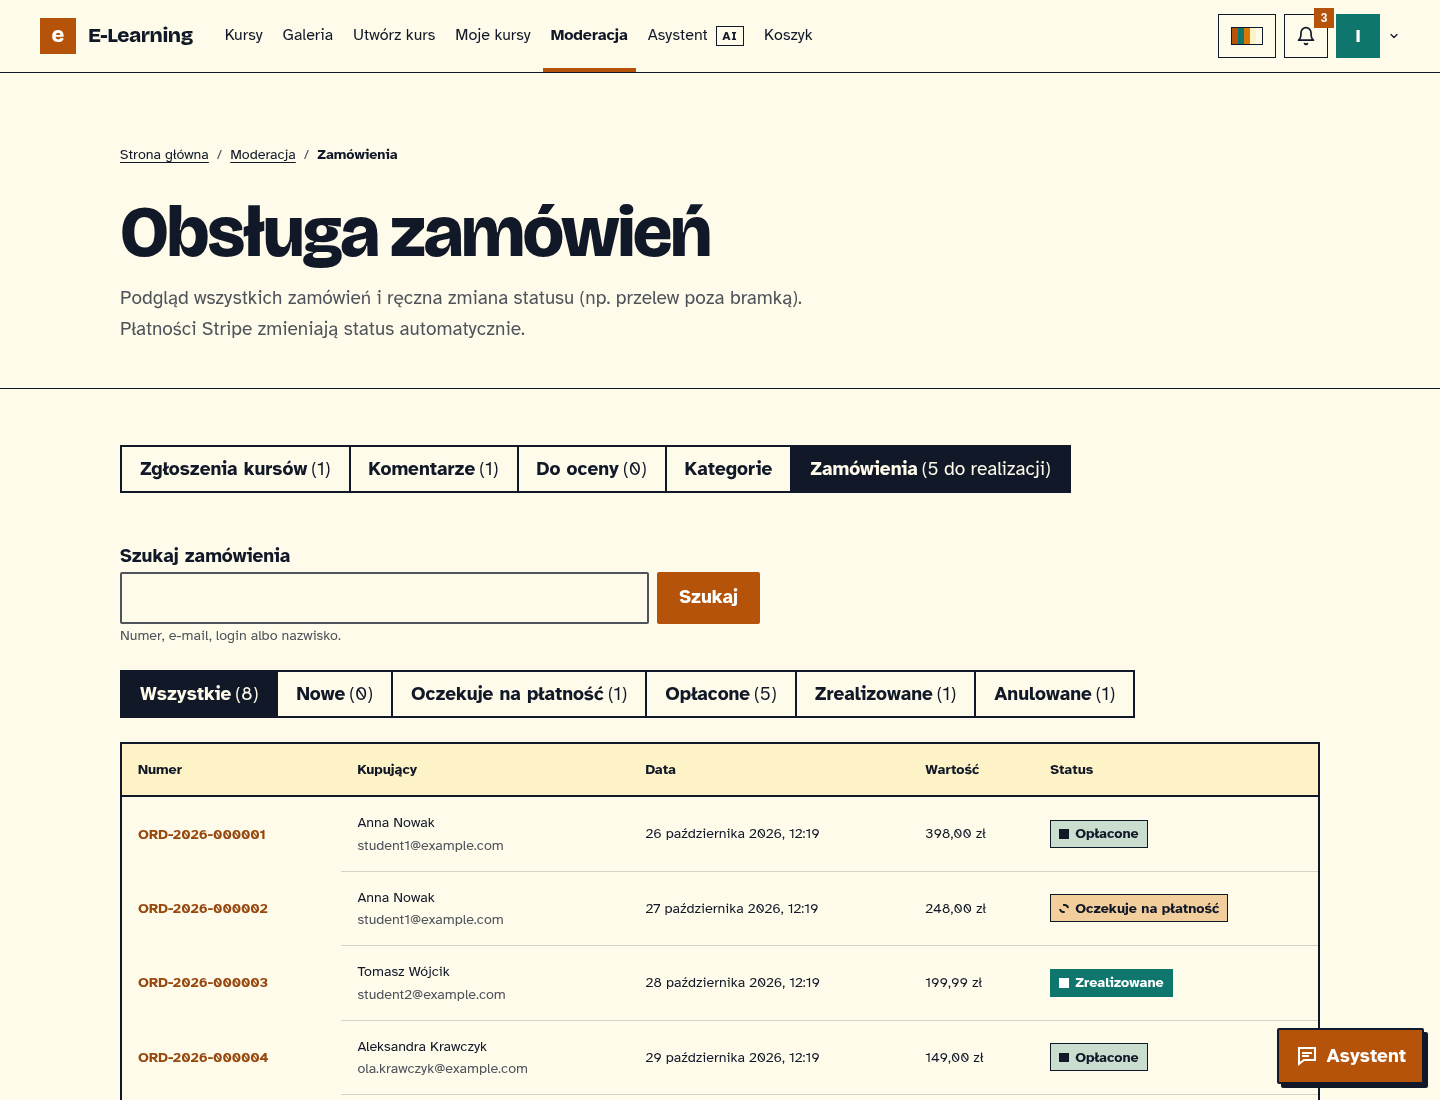
\includegraphics[width=0.94\linewidth,height=0.37\textheight,keepaspectratio]{img/orders_manage.png}}
\caption{Obsługa zamówień}\label{fig:ui-orders-manage}
\end{figure}
Filtr statusu jako przełącznik segmentowy, wyszukiwarka i~tabela z~paginacją.


\begin{figure}[H]
\centering
\fcolorbox{rule}{white}{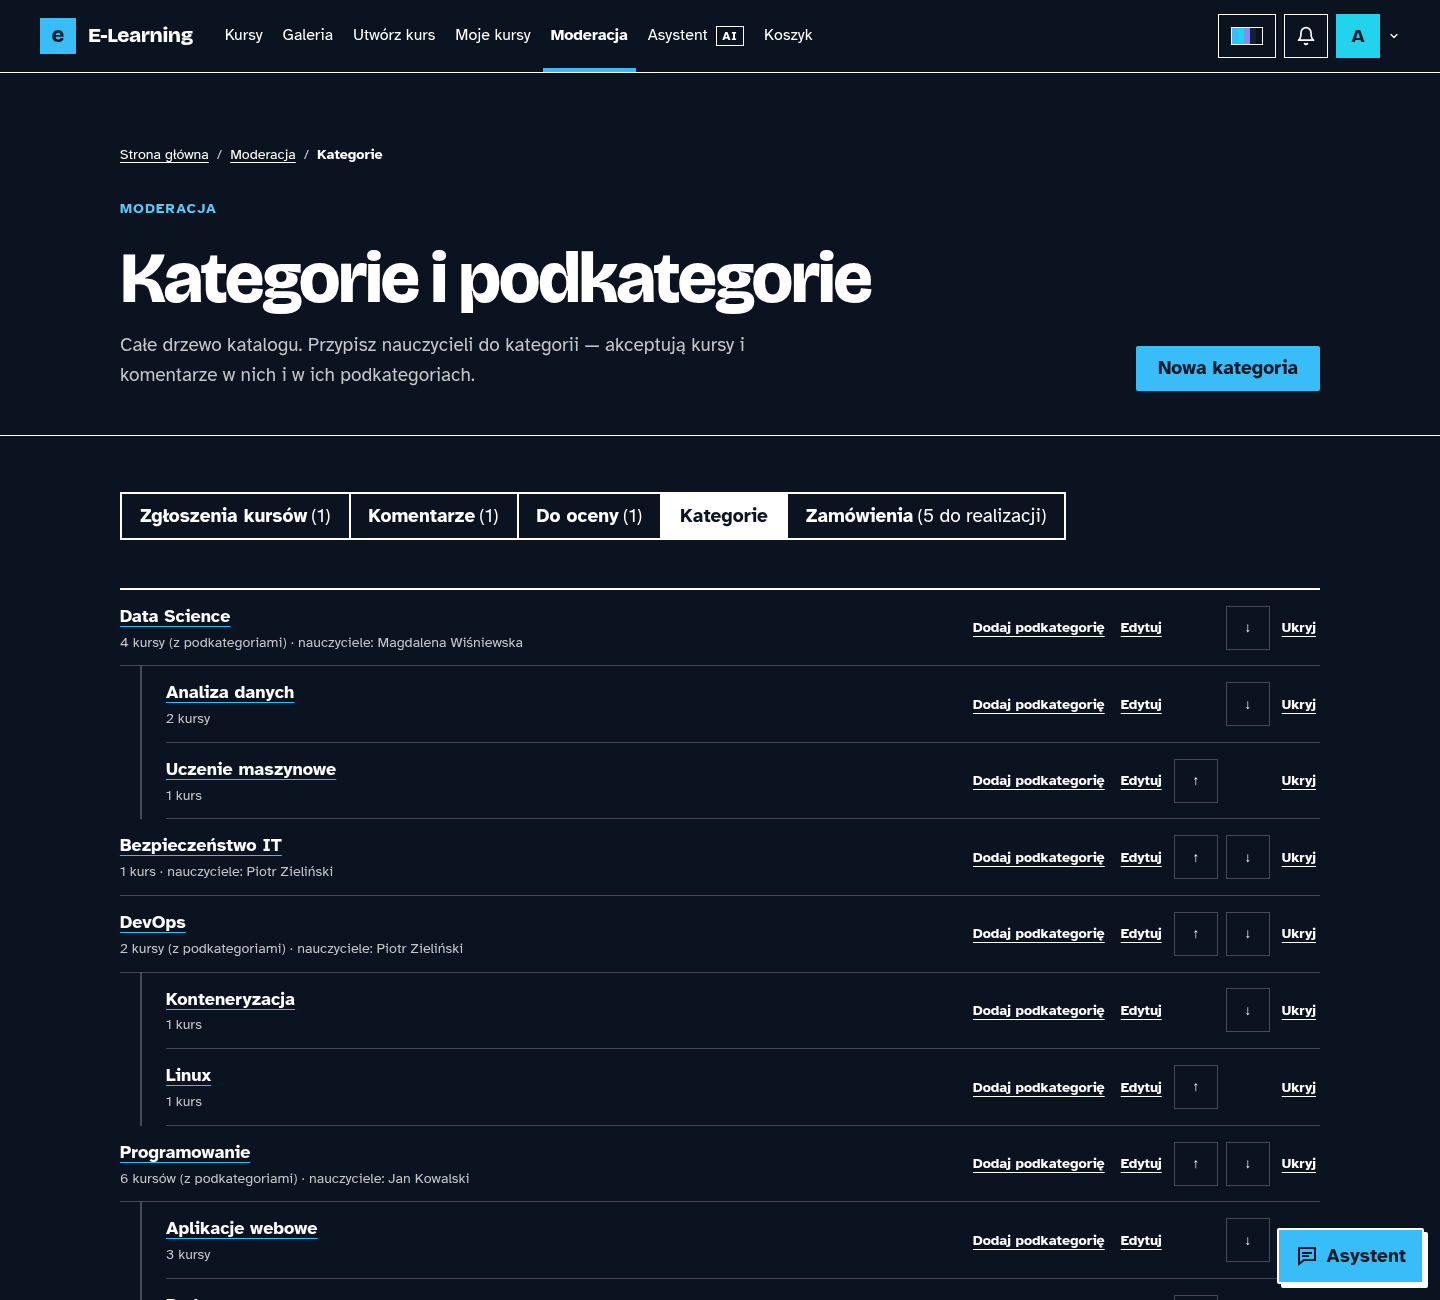
\includegraphics[width=0.94\linewidth,height=0.37\textheight,keepaspectratio]{img/categories.png}}
\caption{Zarządzanie kategoriami (administrator, motyw ciemny ,,Ocean'')}\label{fig:ui-categories}
\end{figure}
Drzewo z~liczbą kursów, dodawanie podkategorii, zmiana kolejności, ukrywanie i~przydział nauczycieli.


\begin{figure}[H]
\centering
\fcolorbox{rule}{white}{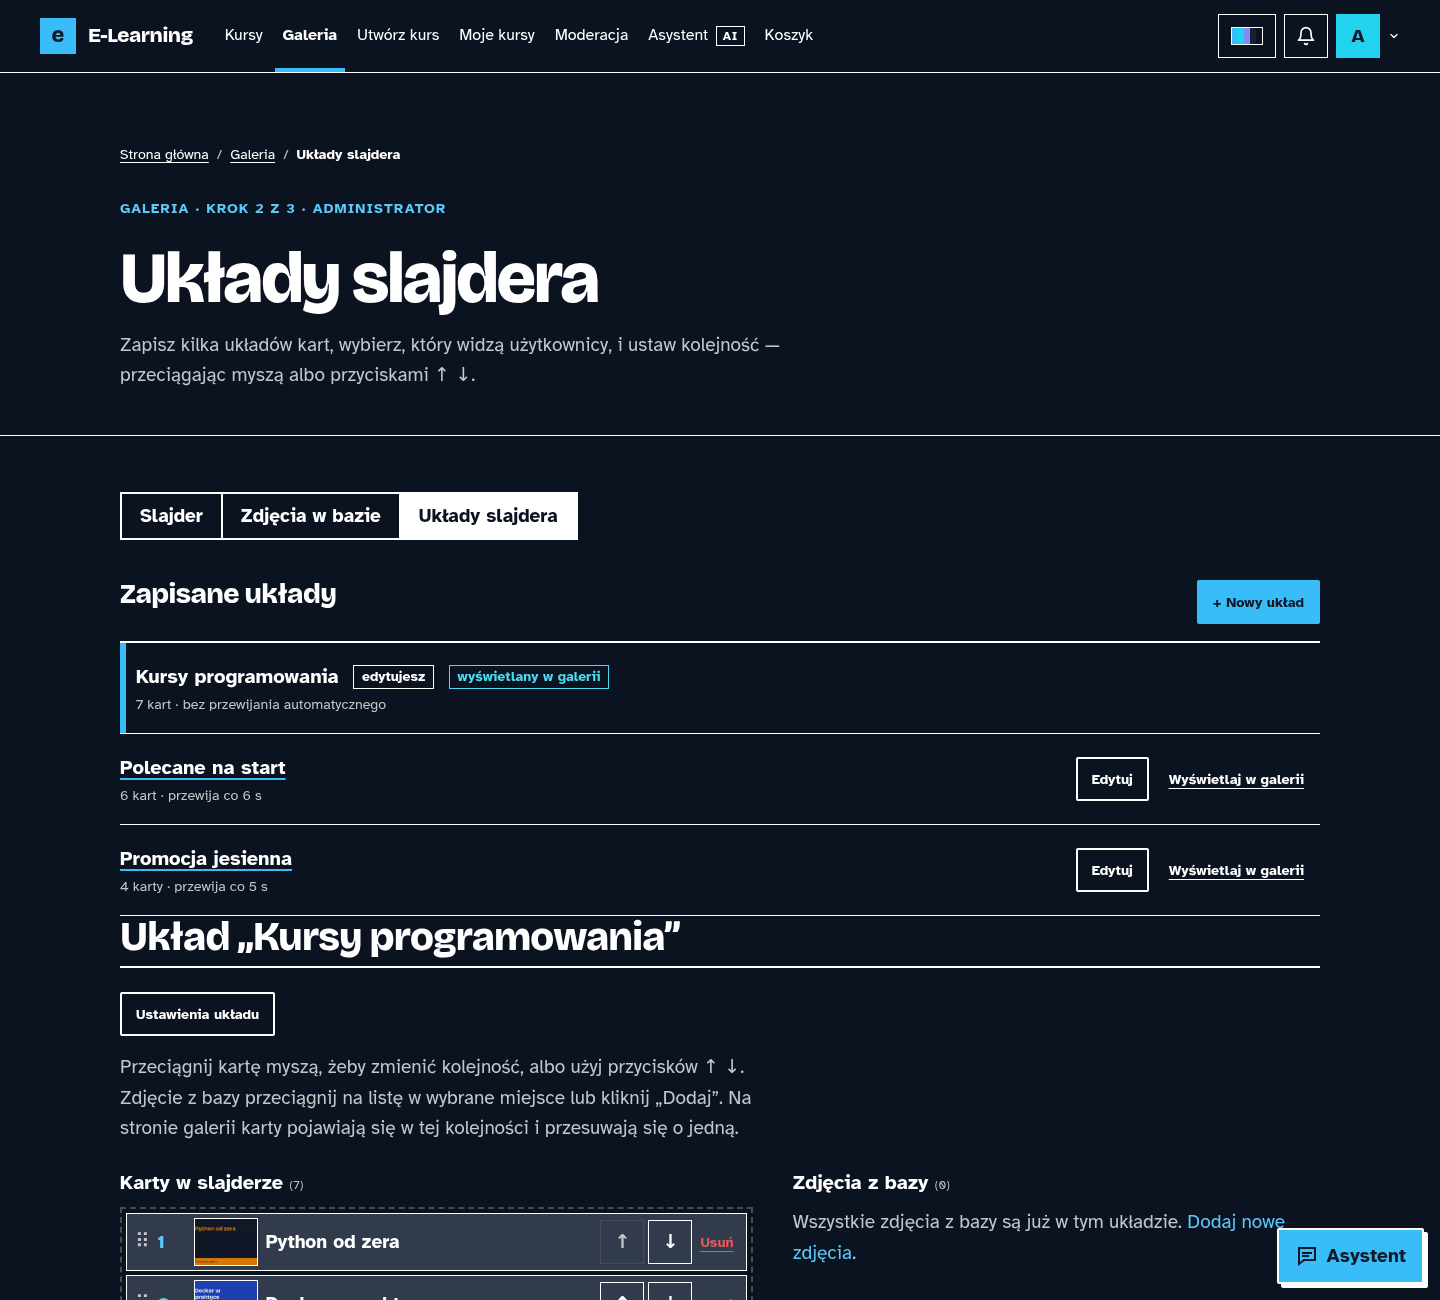
\includegraphics[width=0.94\linewidth,height=0.37\textheight,keepaspectratio]{img/configurator.png}}
\caption{Konfigurator układów slajdera}\label{fig:ui-configurator}
\end{figure}
Lista układów z~oznaczeniem edytowanego i~wyświetlanego; karty przeciągane myszą lub przenoszone przyciskami $\uparrow\downarrow$, obok zdjęcia z~bazy do dodania.


\begin{figure}[H]
\centering
\fcolorbox{rule}{white}{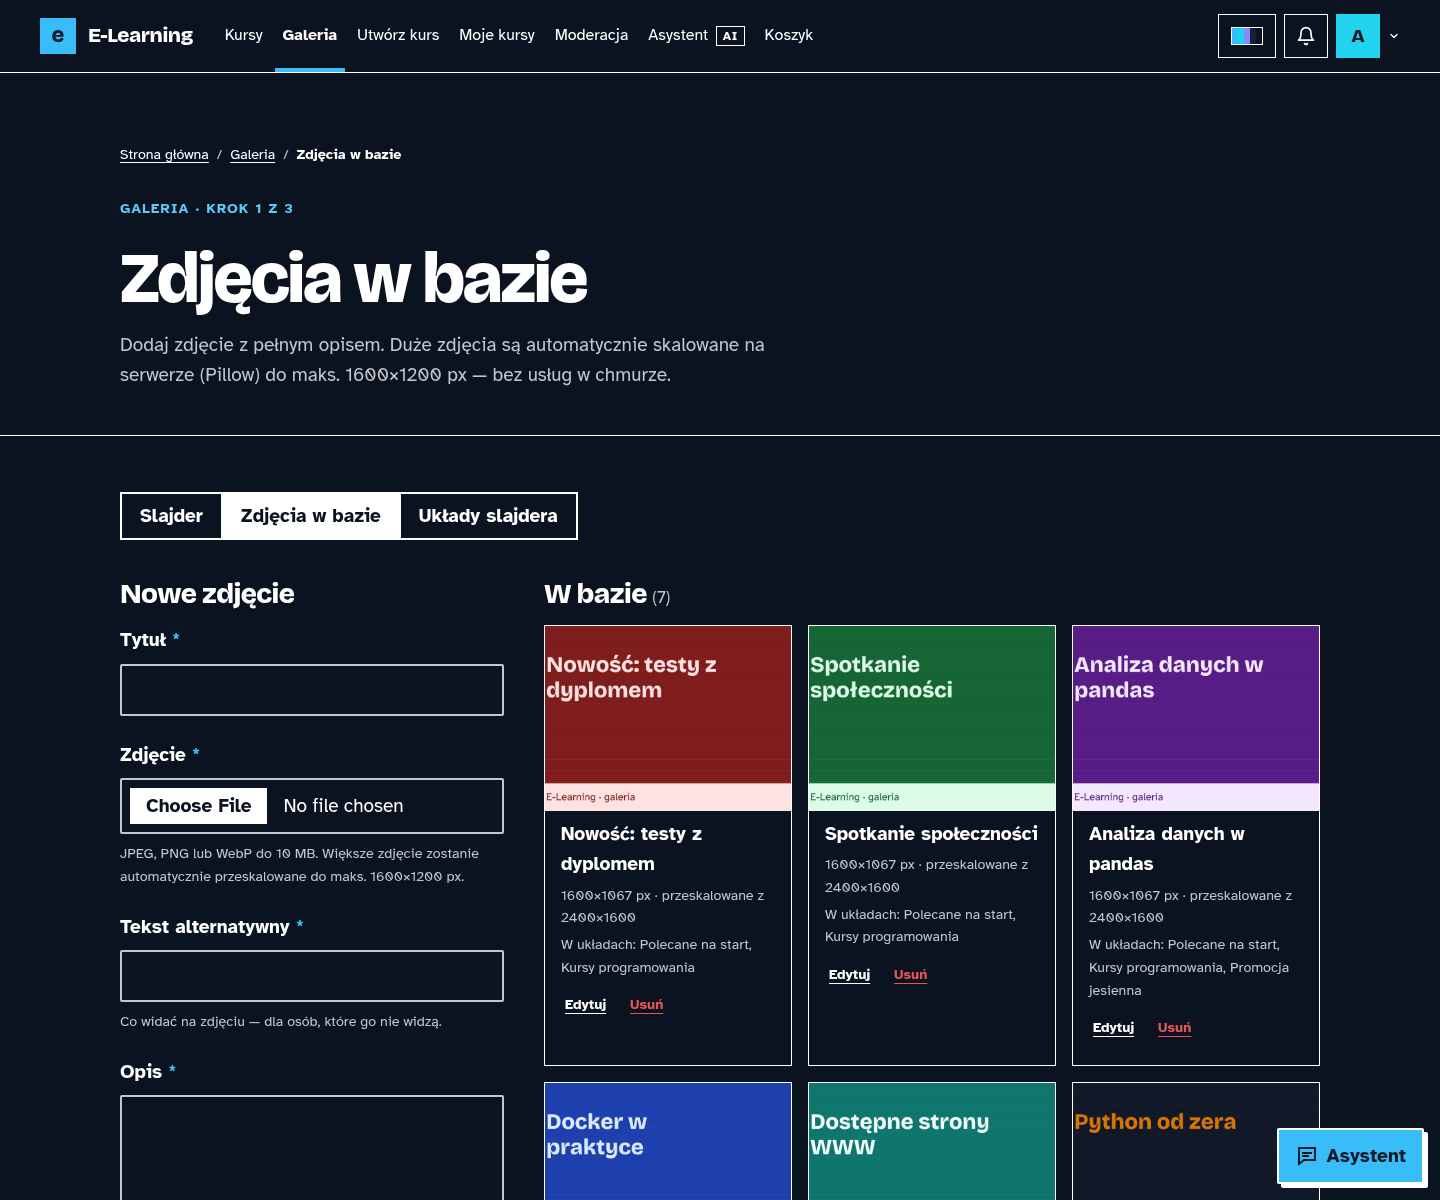
\includegraphics[width=0.94\linewidth,height=0.37\textheight,keepaspectratio]{img/upload.png}}
\caption{Dodawanie zdjęć do galerii}\label{fig:ui-upload}
\end{figure}
Formularz z~wymaganym tekstem alternatywnym i~informacją o~automatycznym skalowaniu; obok baza zdjęć.


\begin{figure}[H]
\centering
\fcolorbox{rule}{white}{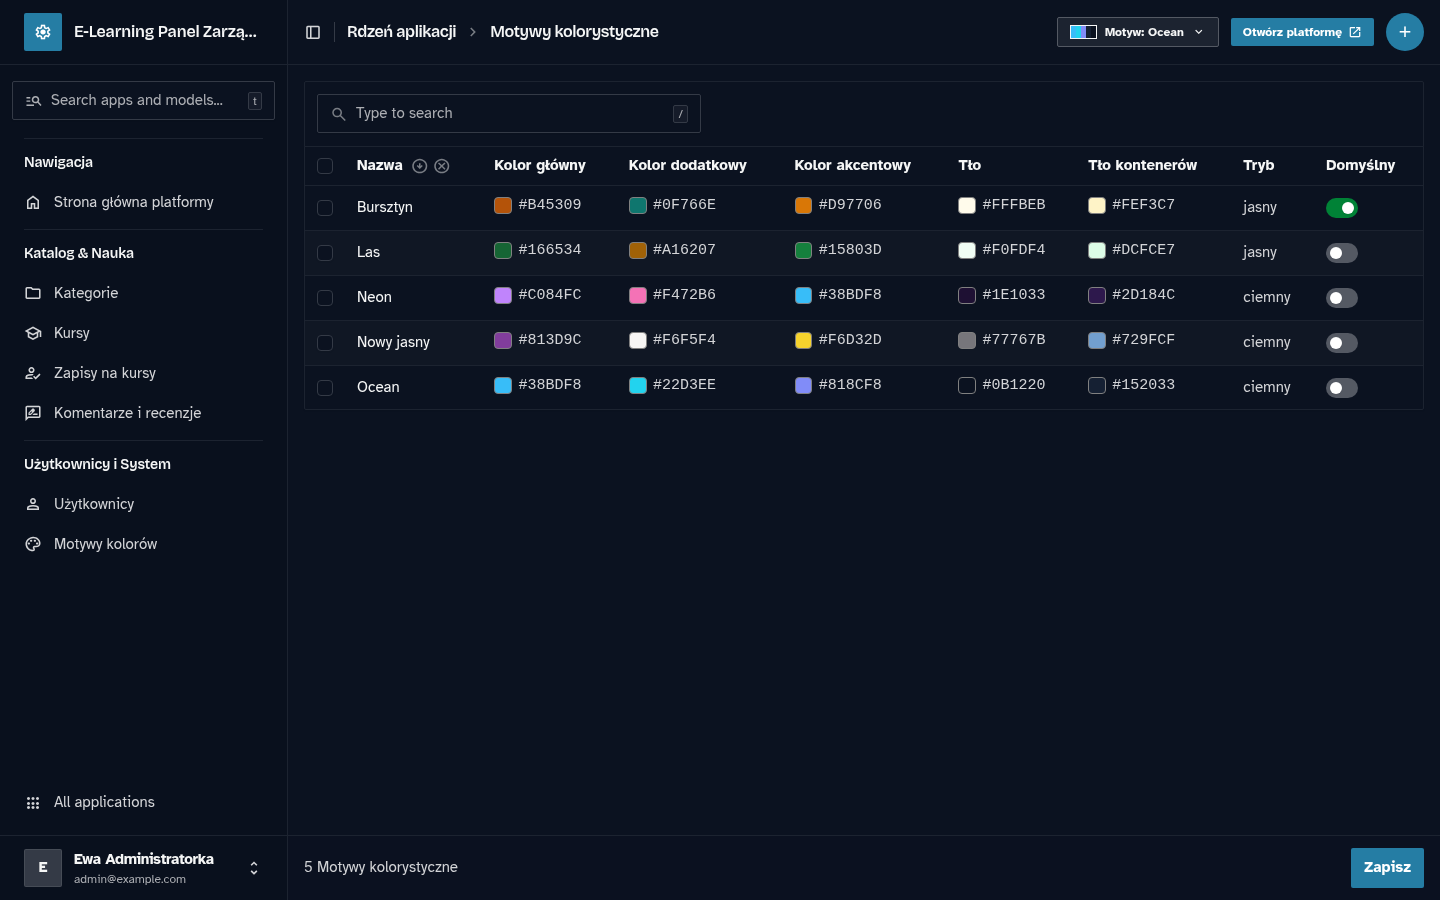
\includegraphics[width=0.94\linewidth,height=0.37\textheight,keepaspectratio]{img/admin_theme.png}}
\caption{Panel administracyjny -- motywy kolorystyczne}\label{fig:ui-admin-theme}
\end{figure}
Panel django-unfold w~kolorach motywu: lista motywów z~pięcioma kolorami, trybem (wyliczonym) i~przełącznikiem motywu domyślnego.


\section{Style uczenia się, ankieta, polecanie, statystyki}
\begin{figure}[H]
\centering
\fcolorbox{rule}{white}{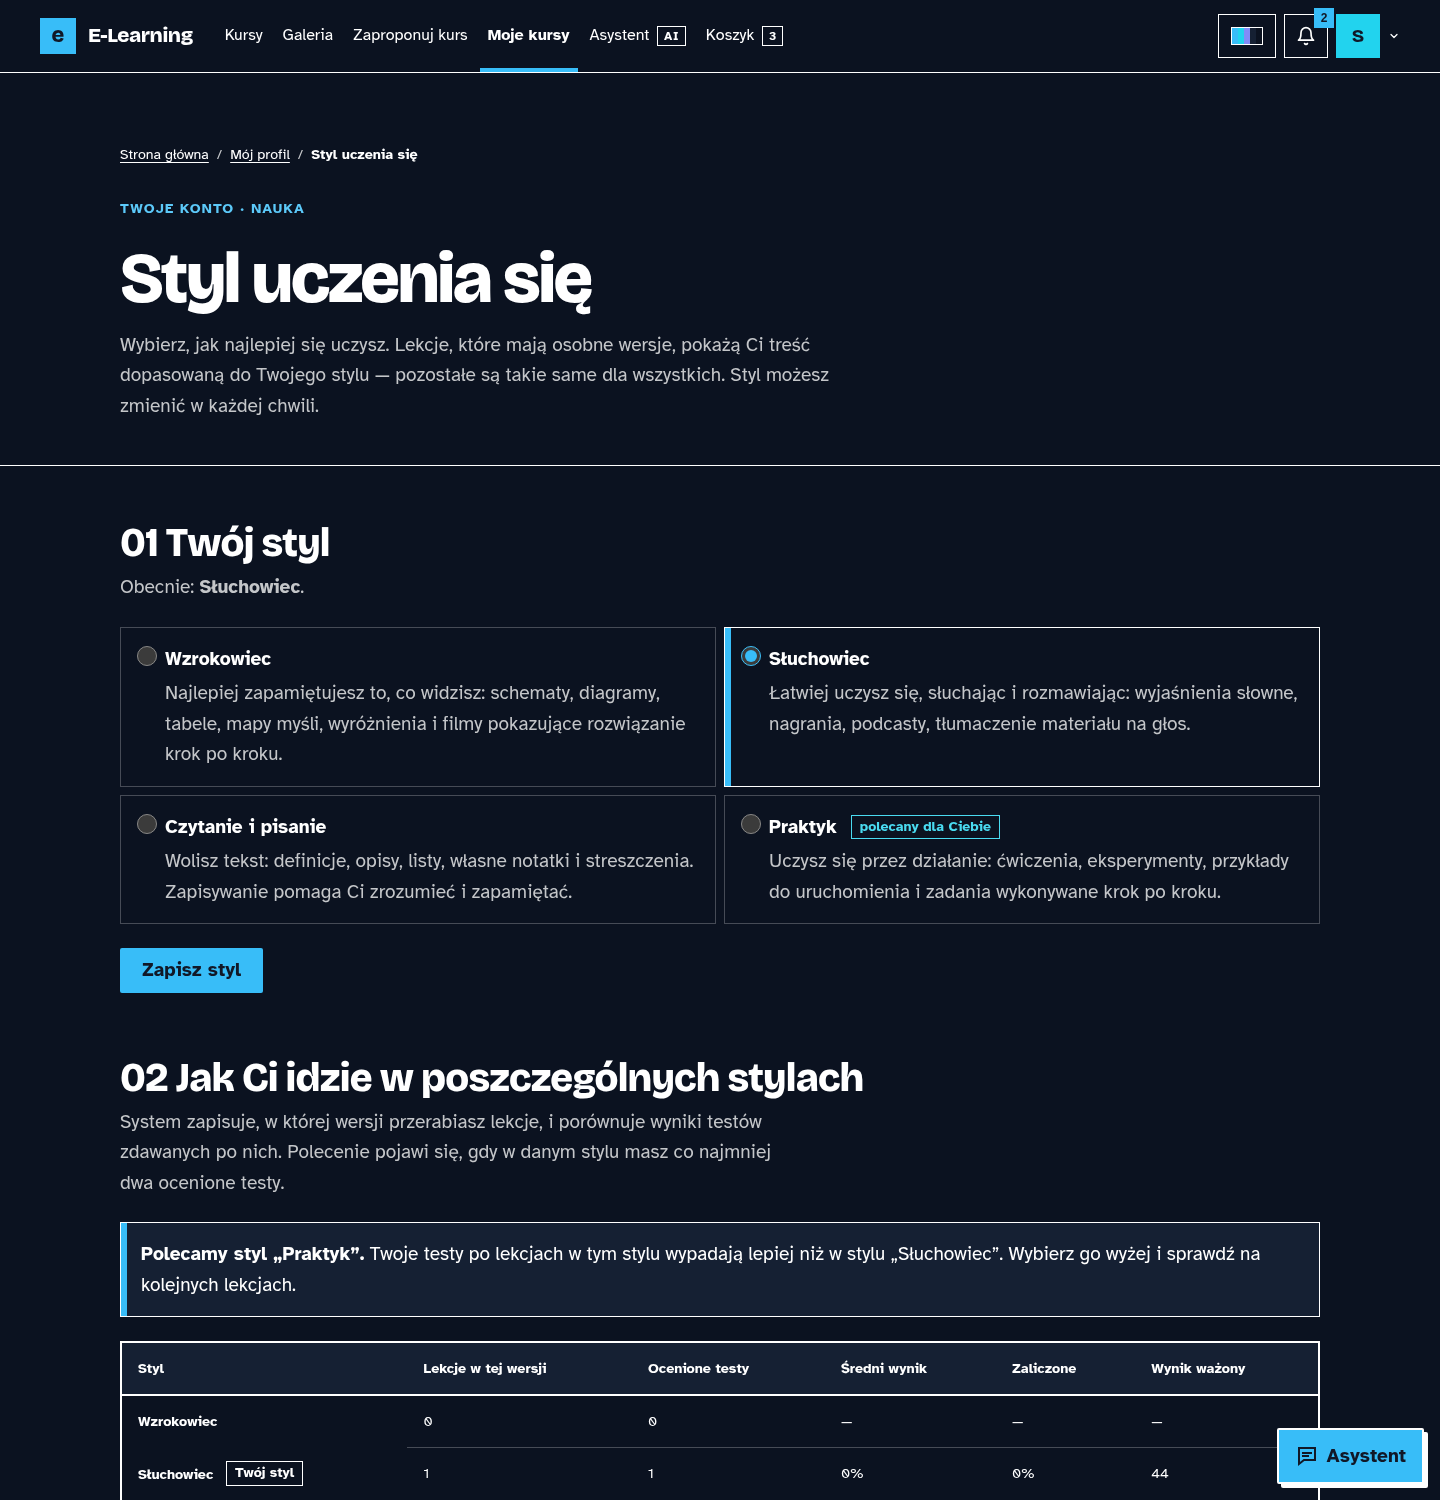
\includegraphics[width=0.94\linewidth,height=0.37\textheight,keepaspectratio]{img/style_student2.png}}
\caption{Strona stylu uczenia się -- uczeń z~rekomendacją zmiany stylu (motyw ciemny)}\label{fig:ui-style}
\end{figure}
Karty wyboru stylu to grupa pól radio w~\code{fieldset}; pod nimi komunikat z~rekomendacją i~tabela wyników w~podziale na style.

\begin{figure}[H]
\centering
\fcolorbox{rule}{white}{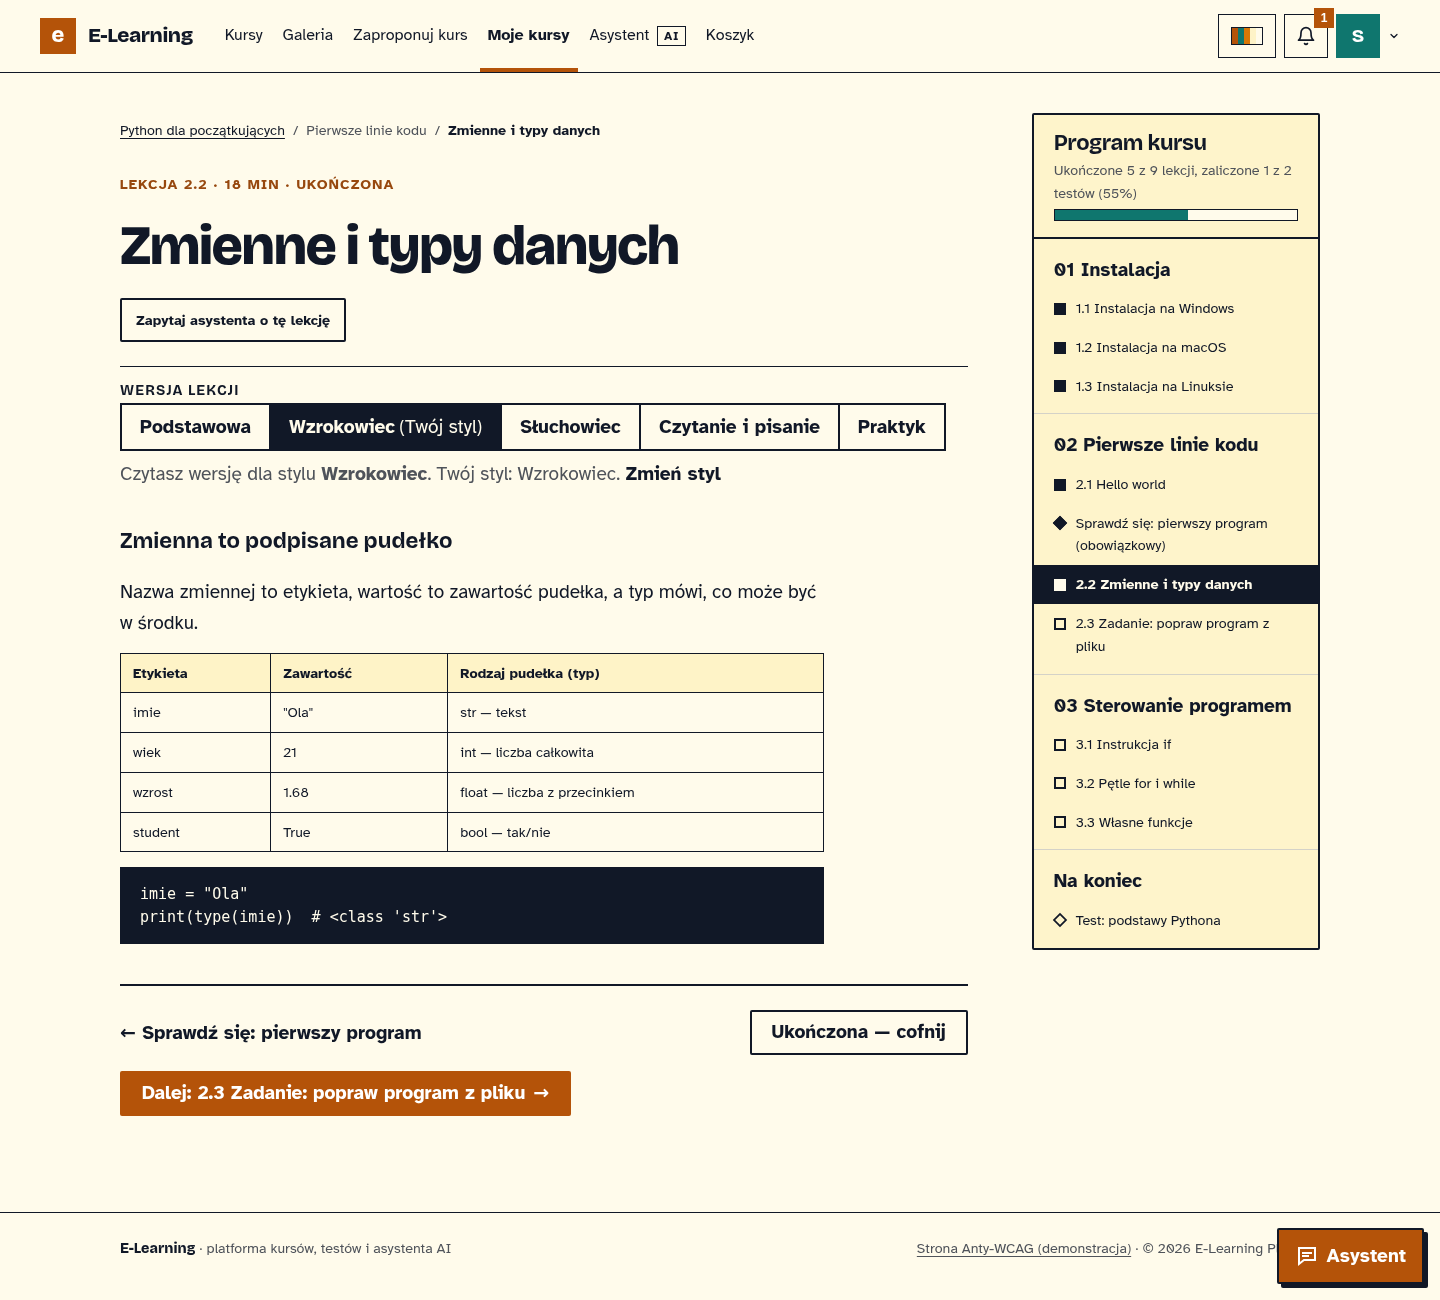
\includegraphics[width=0.94\linewidth,height=0.37\textheight,keepaspectratio]{img/lesson_variant_s1.png}}
\caption{Lekcja w~wersji dla stylu ,,Wzrokowiec'' z~przełącznikiem wersji}\label{fig:ui-variant}
\end{figure}
Przełącznik wersji to nawigacja z~linkami (\code{aria-current} na wyświetlanej wersji); wersja stylu ucznia jest oznaczona ,,(Twój styl)''.

\begin{figure}[H]
\centering
\fcolorbox{rule}{white}{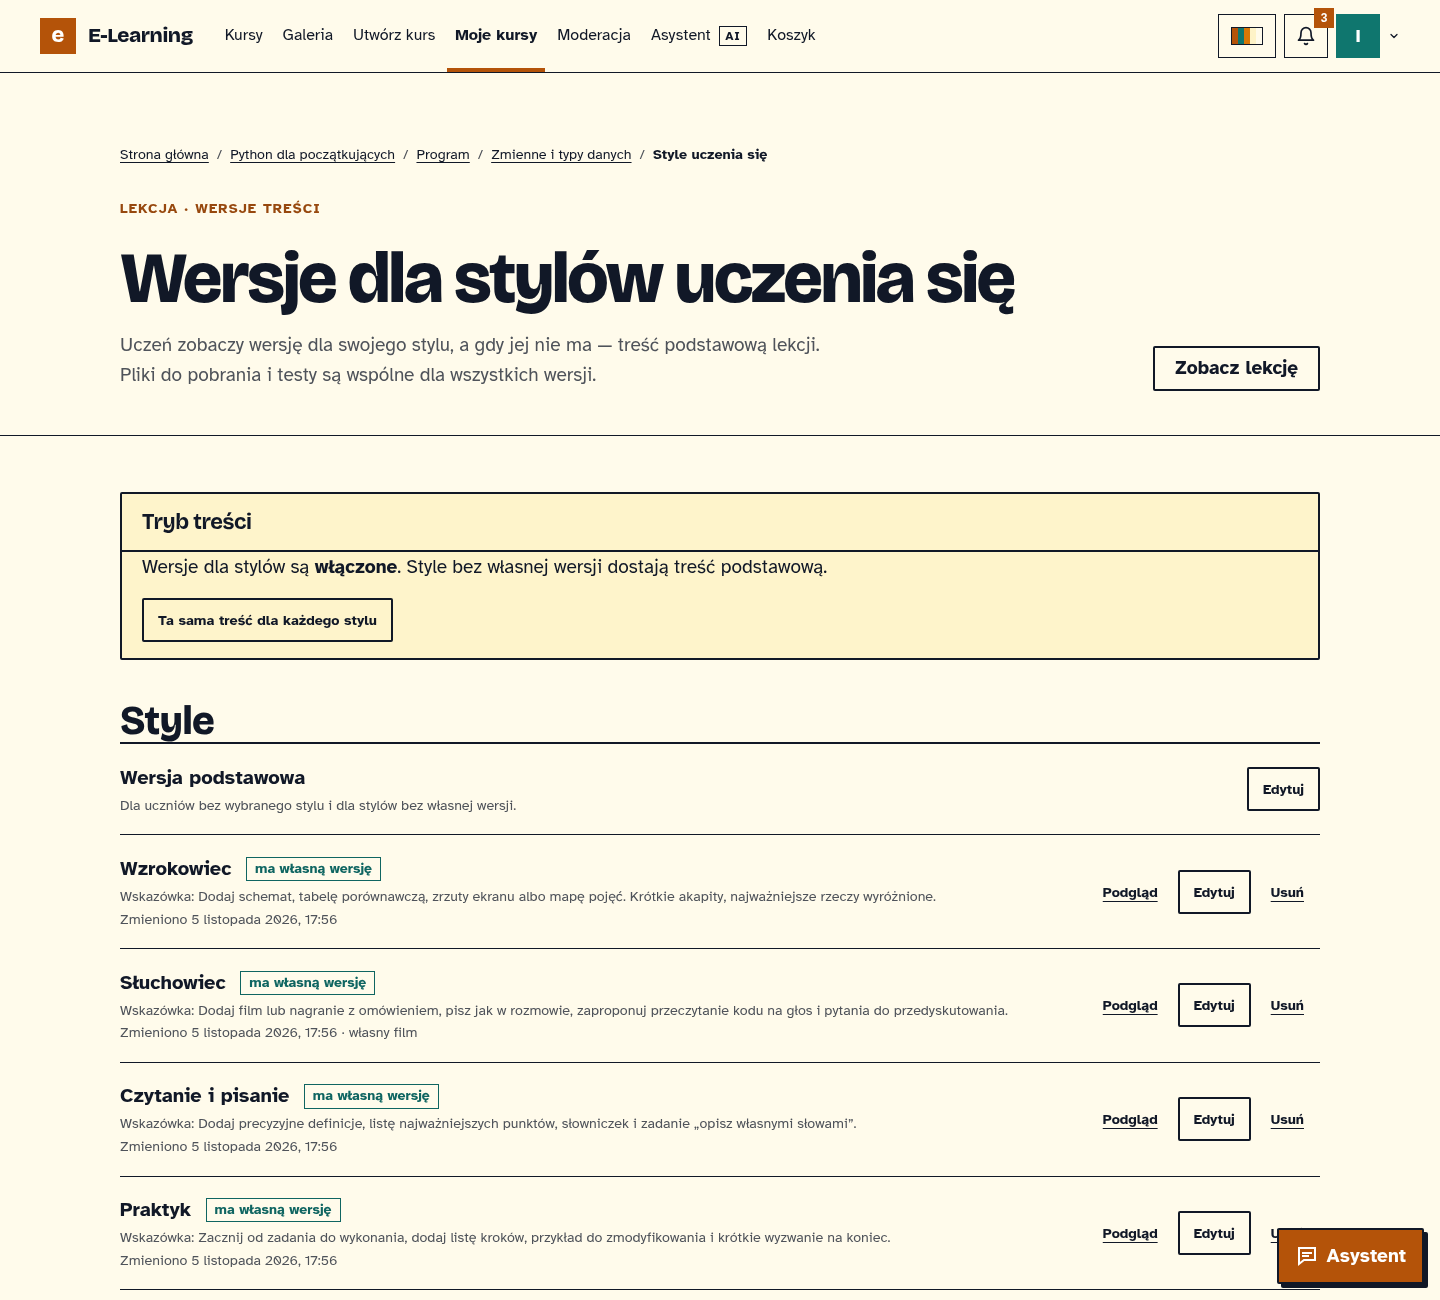
\includegraphics[width=0.94\linewidth,height=0.37\textheight,keepaspectratio]{img/variants_list.png}}
\caption{Autor kursu -- wersje lekcji dla stylów}\label{fig:ui-variants}
\end{figure}
Dla każdego stylu: stan (własna wersja albo treść podstawowa), wskazówka dla autora i~akcje podglądu, edycji oraz usunięcia z~dialogiem potwierdzenia.

\begin{figure}[H]
\centering
\fcolorbox{rule}{white}{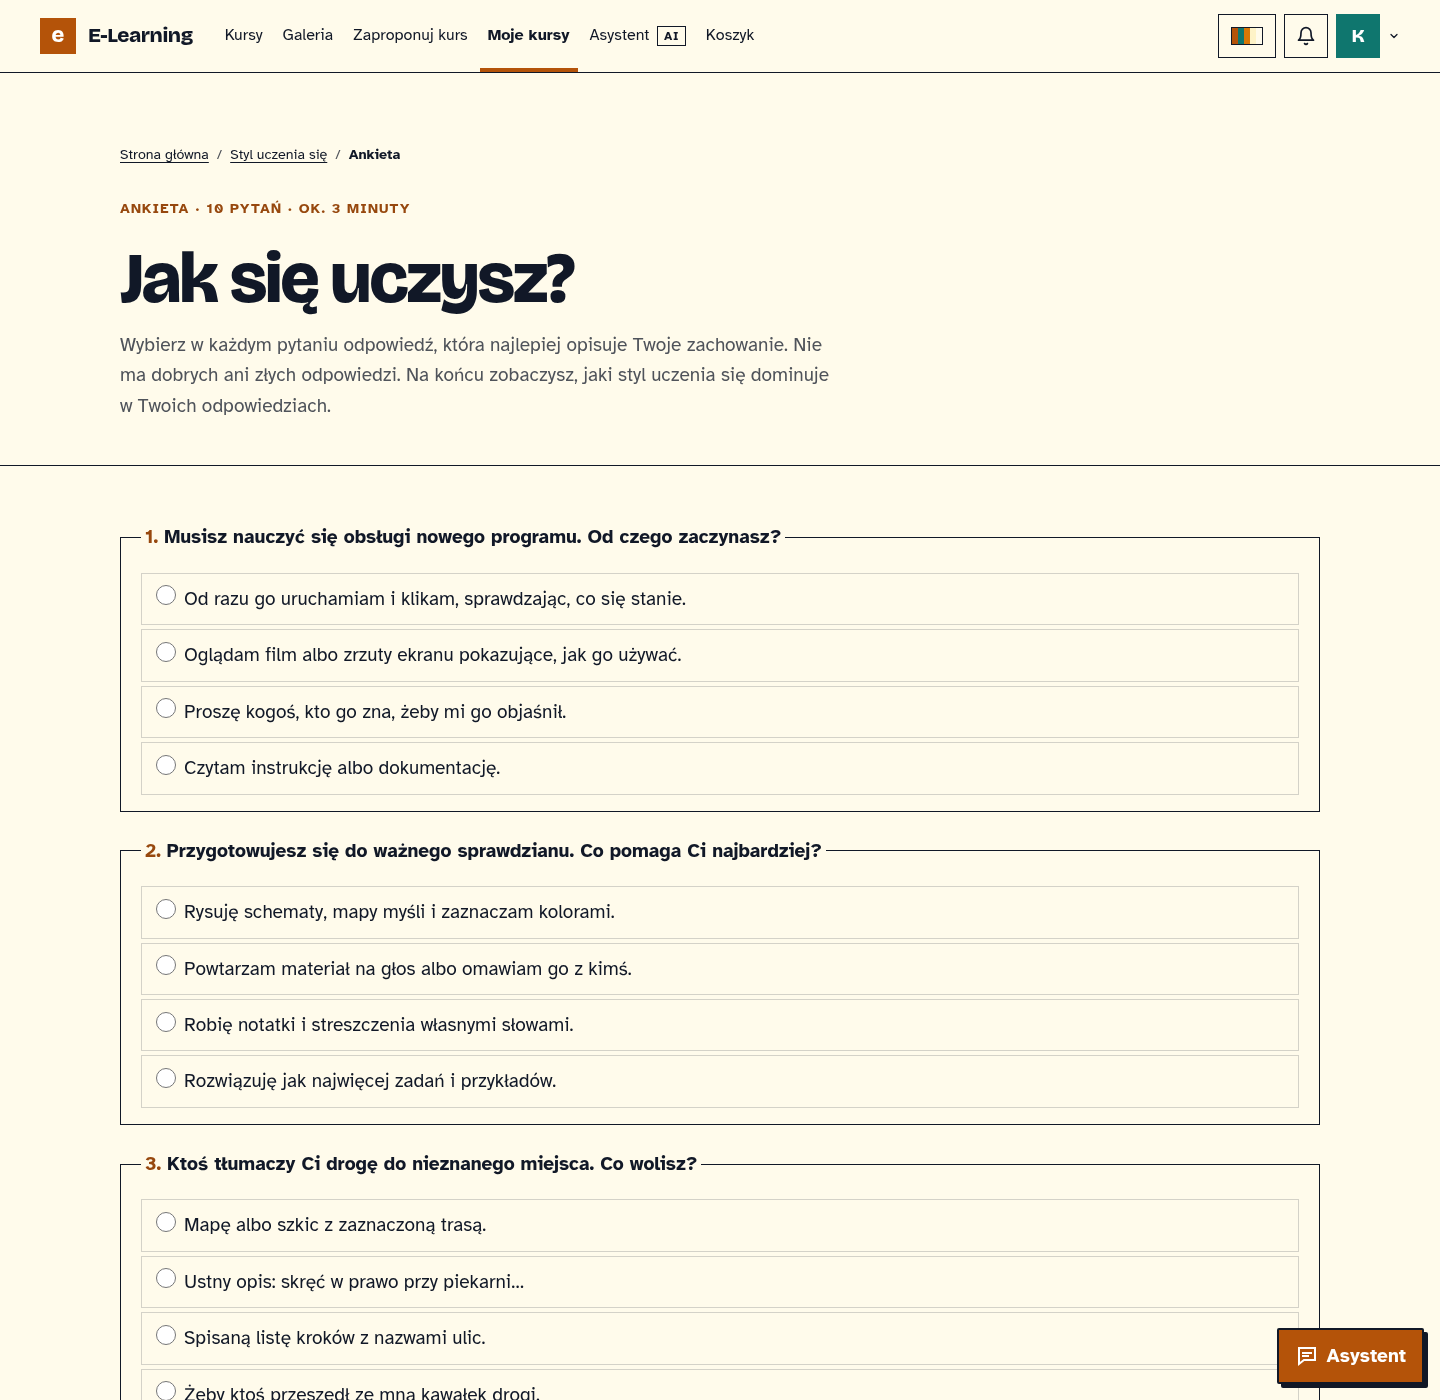
\includegraphics[width=0.94\linewidth,height=0.37\textheight,keepaspectratio]{img/n_survey.png}}
\caption{Ankieta stylu uczenia się}\label{fig:ui-survey}
\end{figure}
Dziesięć pytań sytuacyjnych; każde to grupa pól radio z~legendą, błędy opisane przy pytaniu.

\begin{figure}[H]
\centering
\fcolorbox{rule}{white}{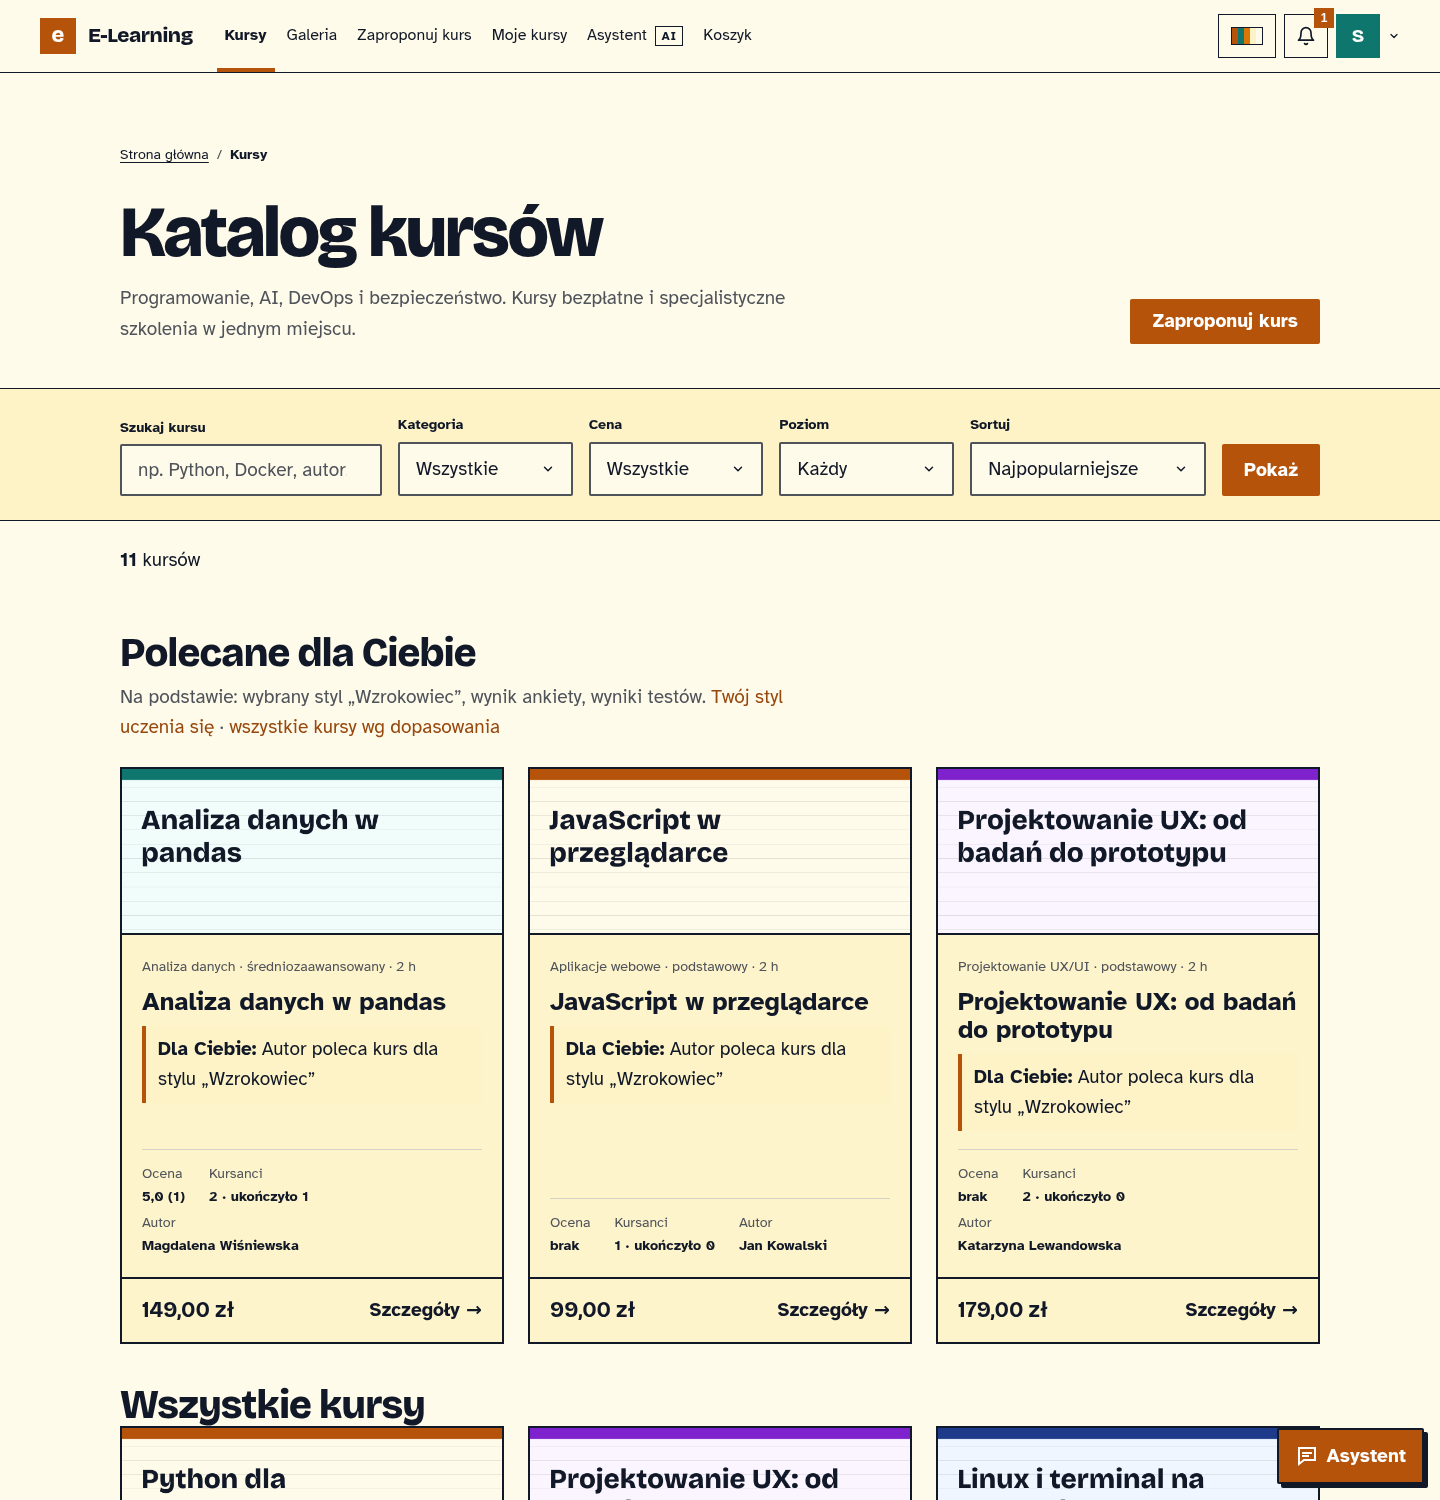
\includegraphics[width=0.94\linewidth,height=0.37\textheight,keepaspectratio]{img/n_catalog.png}}
\caption{Katalog -- sekcja ,,Polecane dla Ciebie''}\label{fig:ui-recommended}
\end{figure}
Nad listą kursów trzy polecenia z~uzasadnieniem (,,Dla Ciebie: …'') i~informacją, z~czego wynika profil; w~sortowaniu opcja ,,Dopasowane do mnie''.

\begin{figure}[H]
\centering
\fcolorbox{rule}{white}{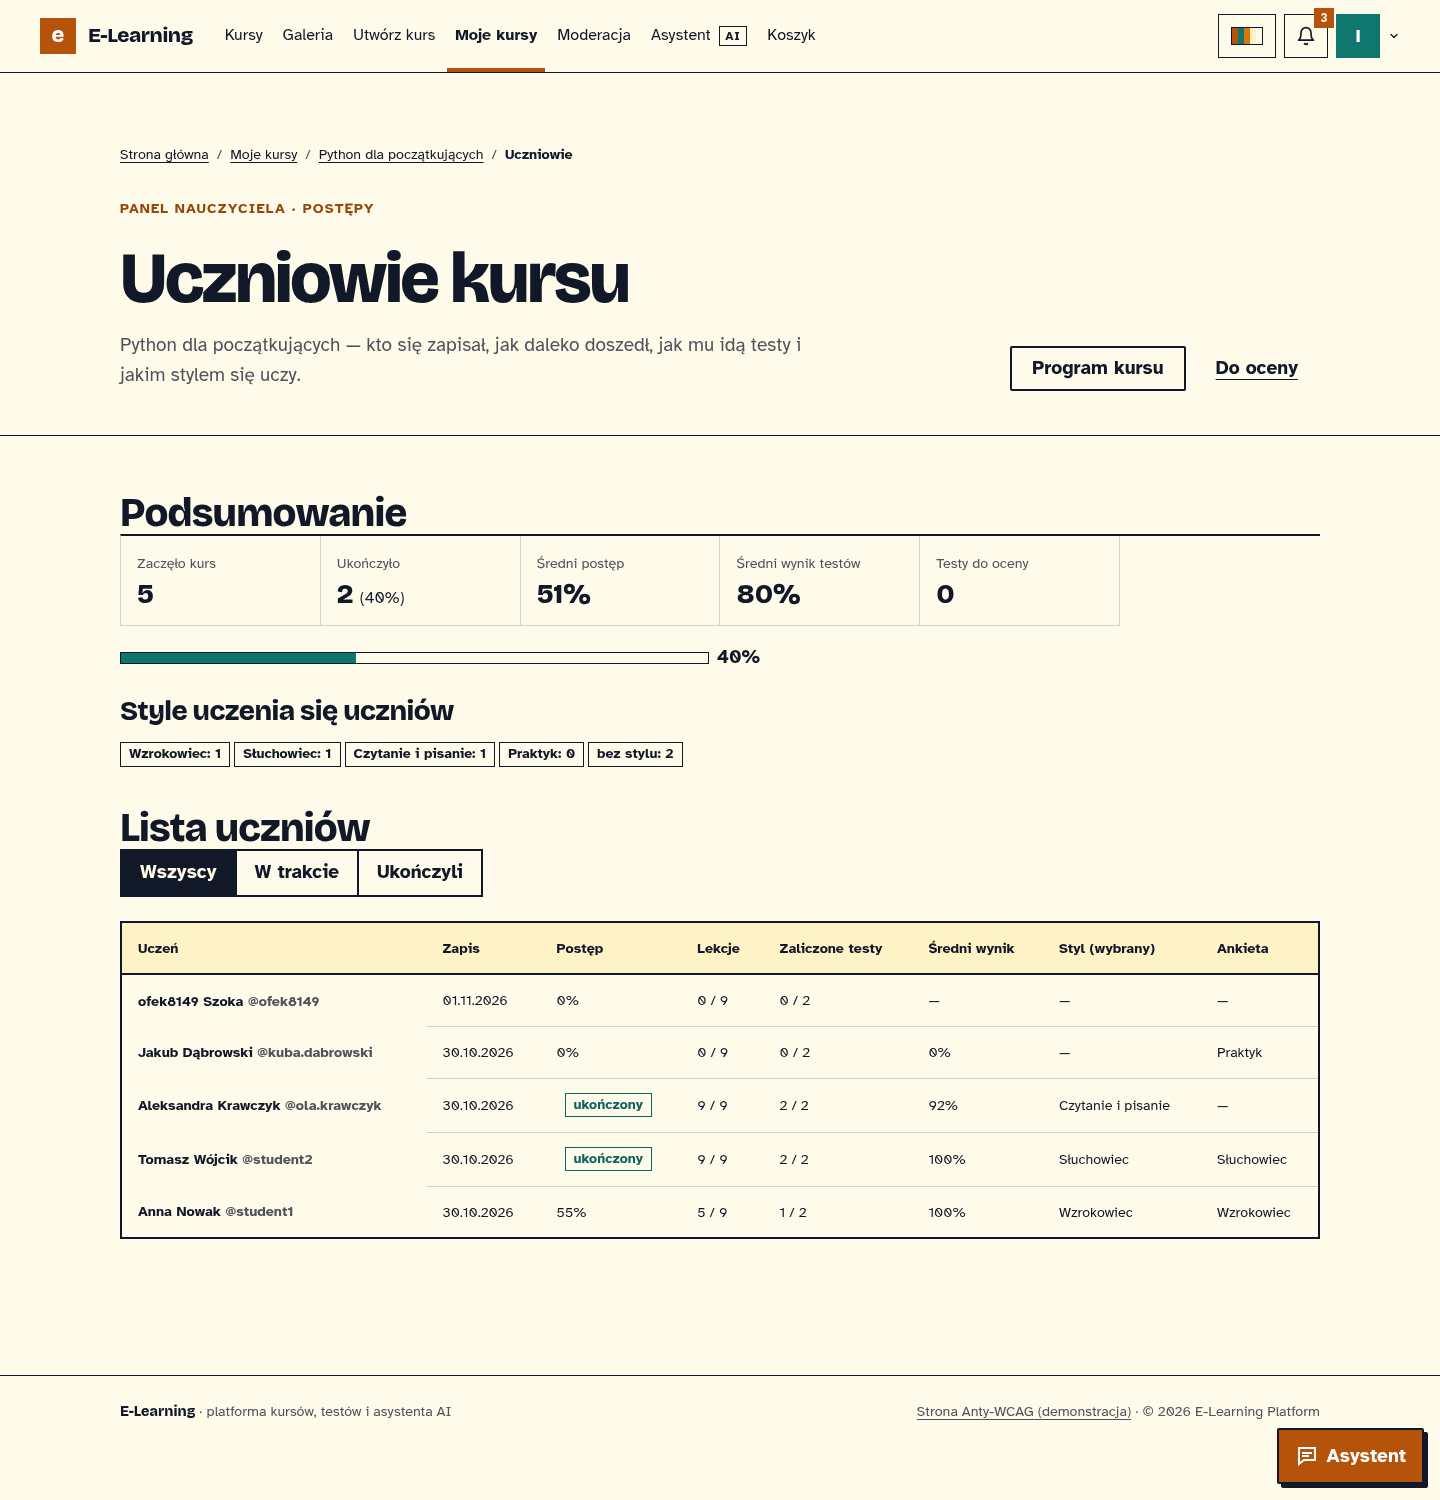
\includegraphics[width=0.94\linewidth,height=0.37\textheight,keepaspectratio]{img/n_students.png}}
\caption{Panel nauczyciela -- uczniowie kursu}\label{fig:ui-students}
\end{figure}
Podsumowanie (zaczęło, ukończyło, procent ukończenia, średni postęp i~wynik), rozkład stylów i~tabela uczniów z~filtrem.

\begin{figure}[H]
\centering
\fcolorbox{rule}{white}{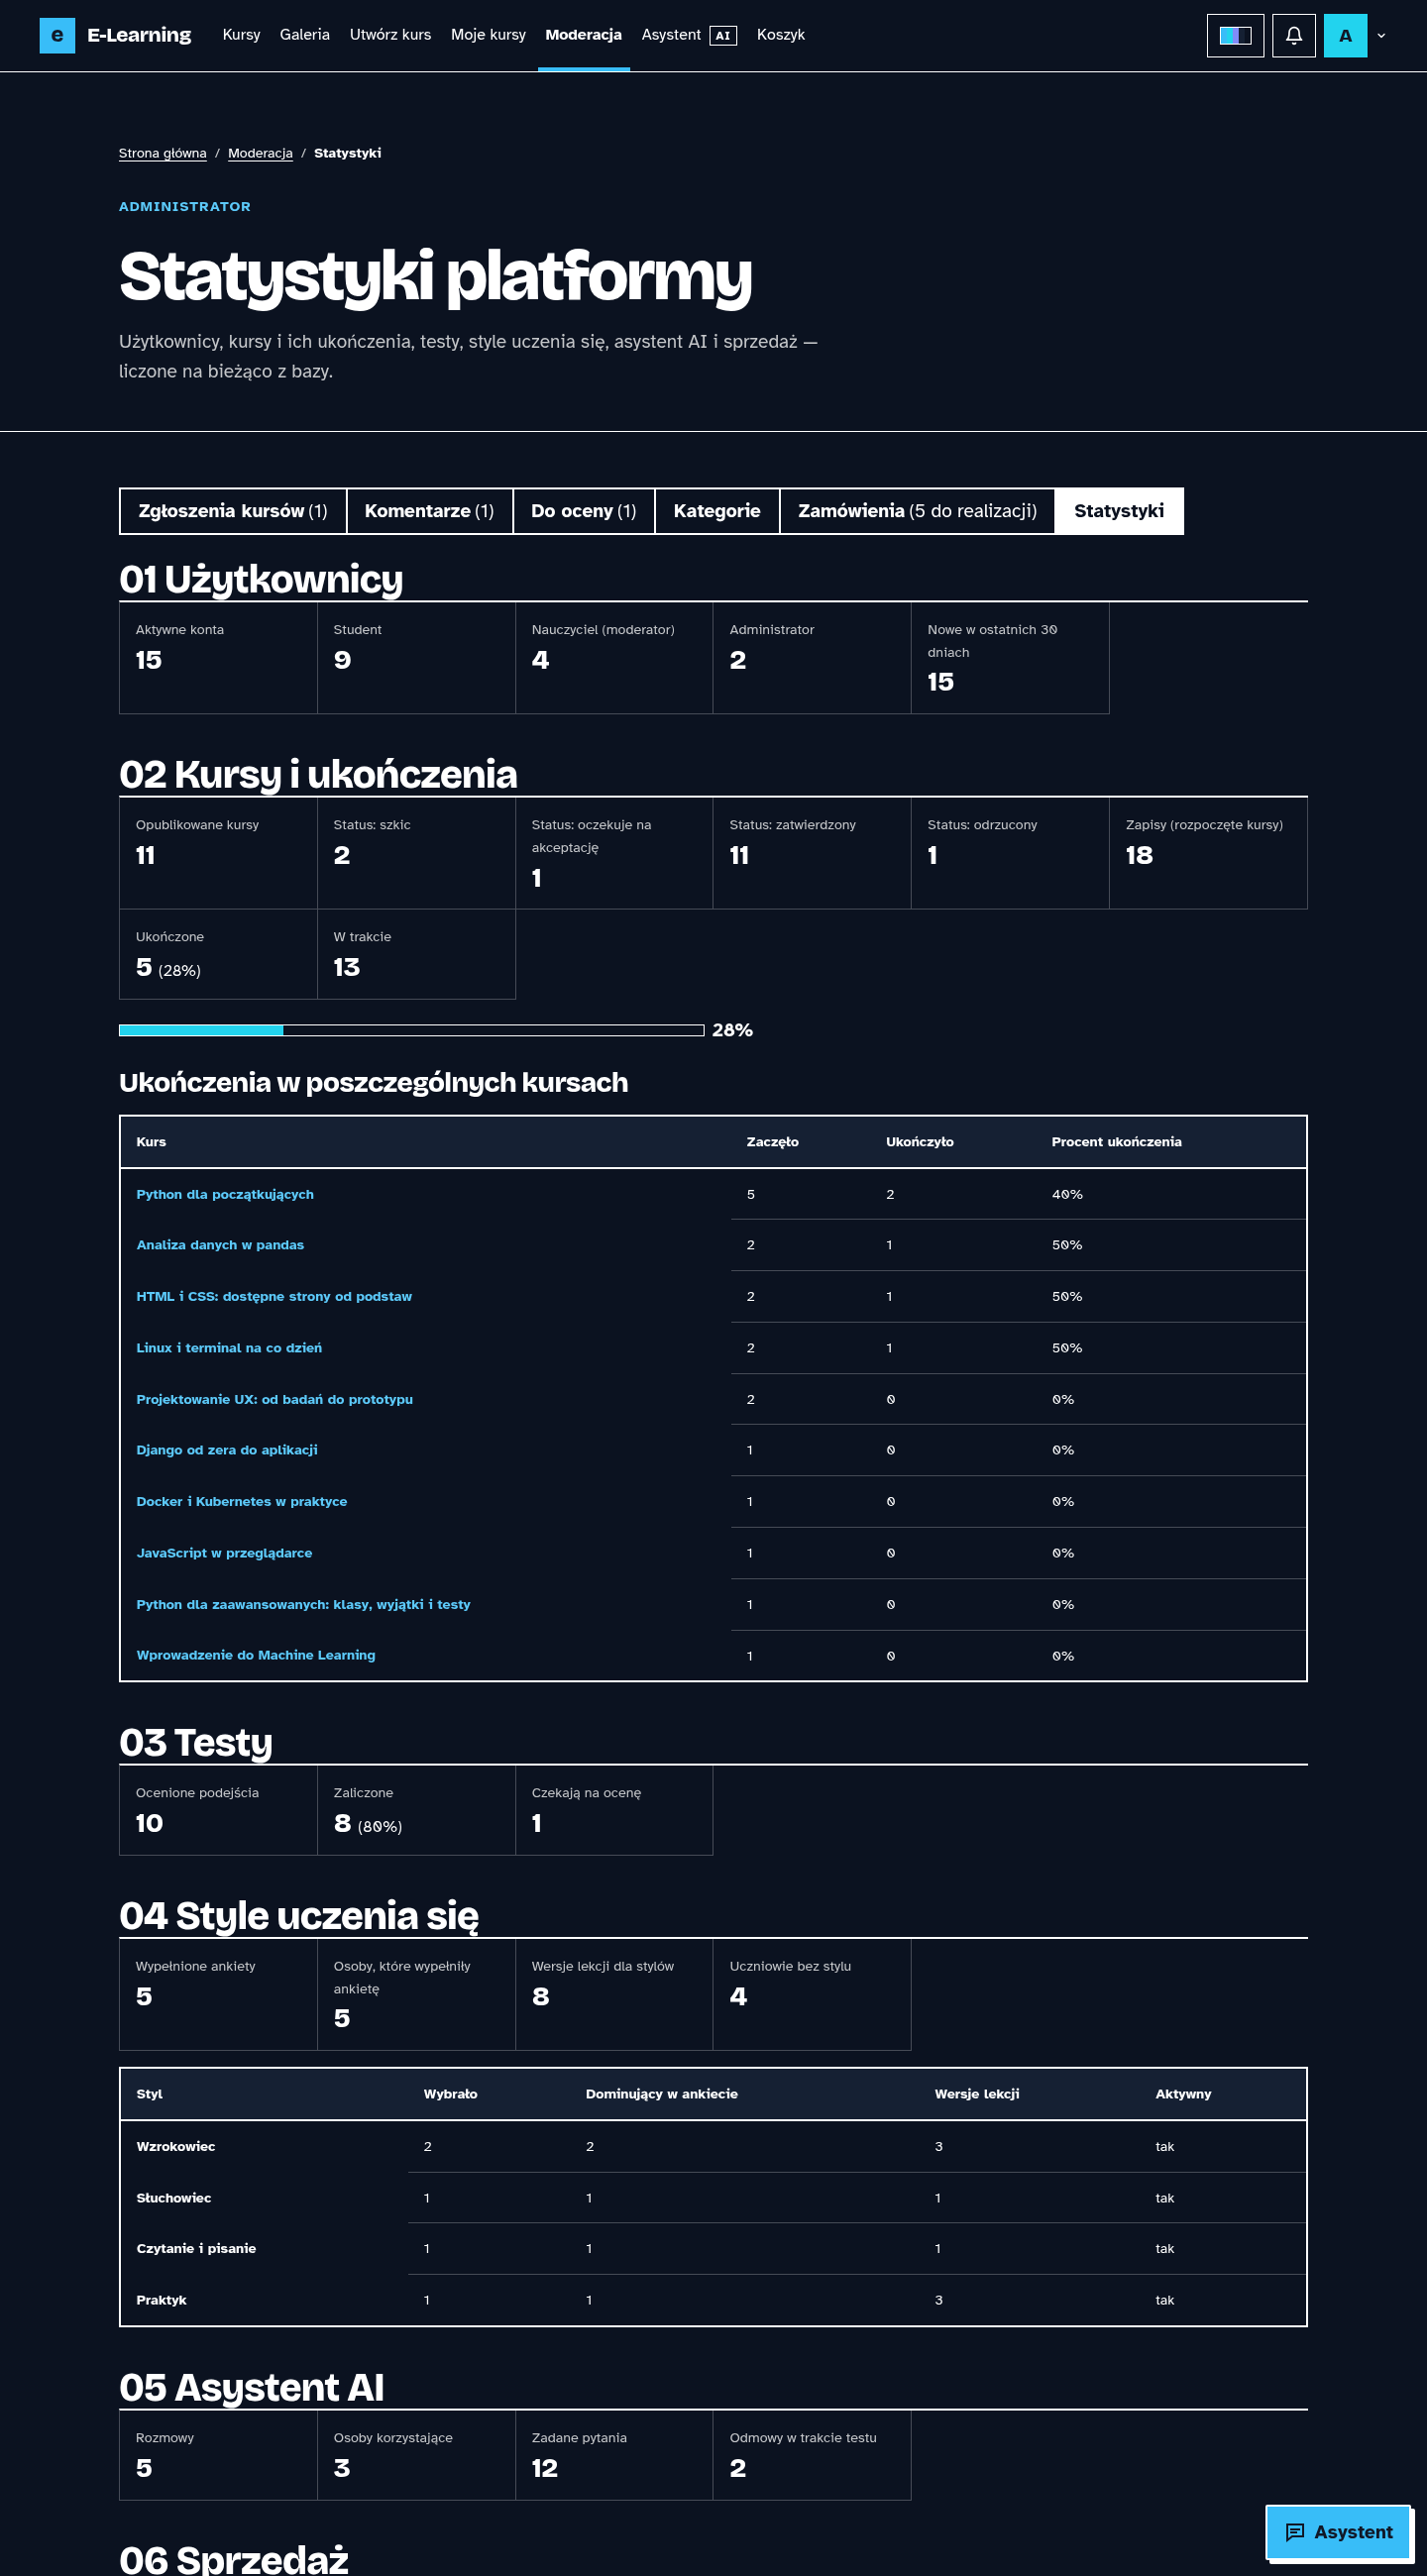
\includegraphics[width=0.94\linewidth,height=0.37\textheight,keepaspectratio]{img/n_stats.png}}
\caption{Statystyki platformy (administrator, motyw ,,Ocean'')}\label{fig:ui-stats}
\end{figure}
Liczby z~bazy w~sześciu obszarach; tabela ukończeń w~każdym kursie z~procentem ukończenia.

\section{Galeria}

\begin{figure}[H]
\centering
\fcolorbox{rule}{white}{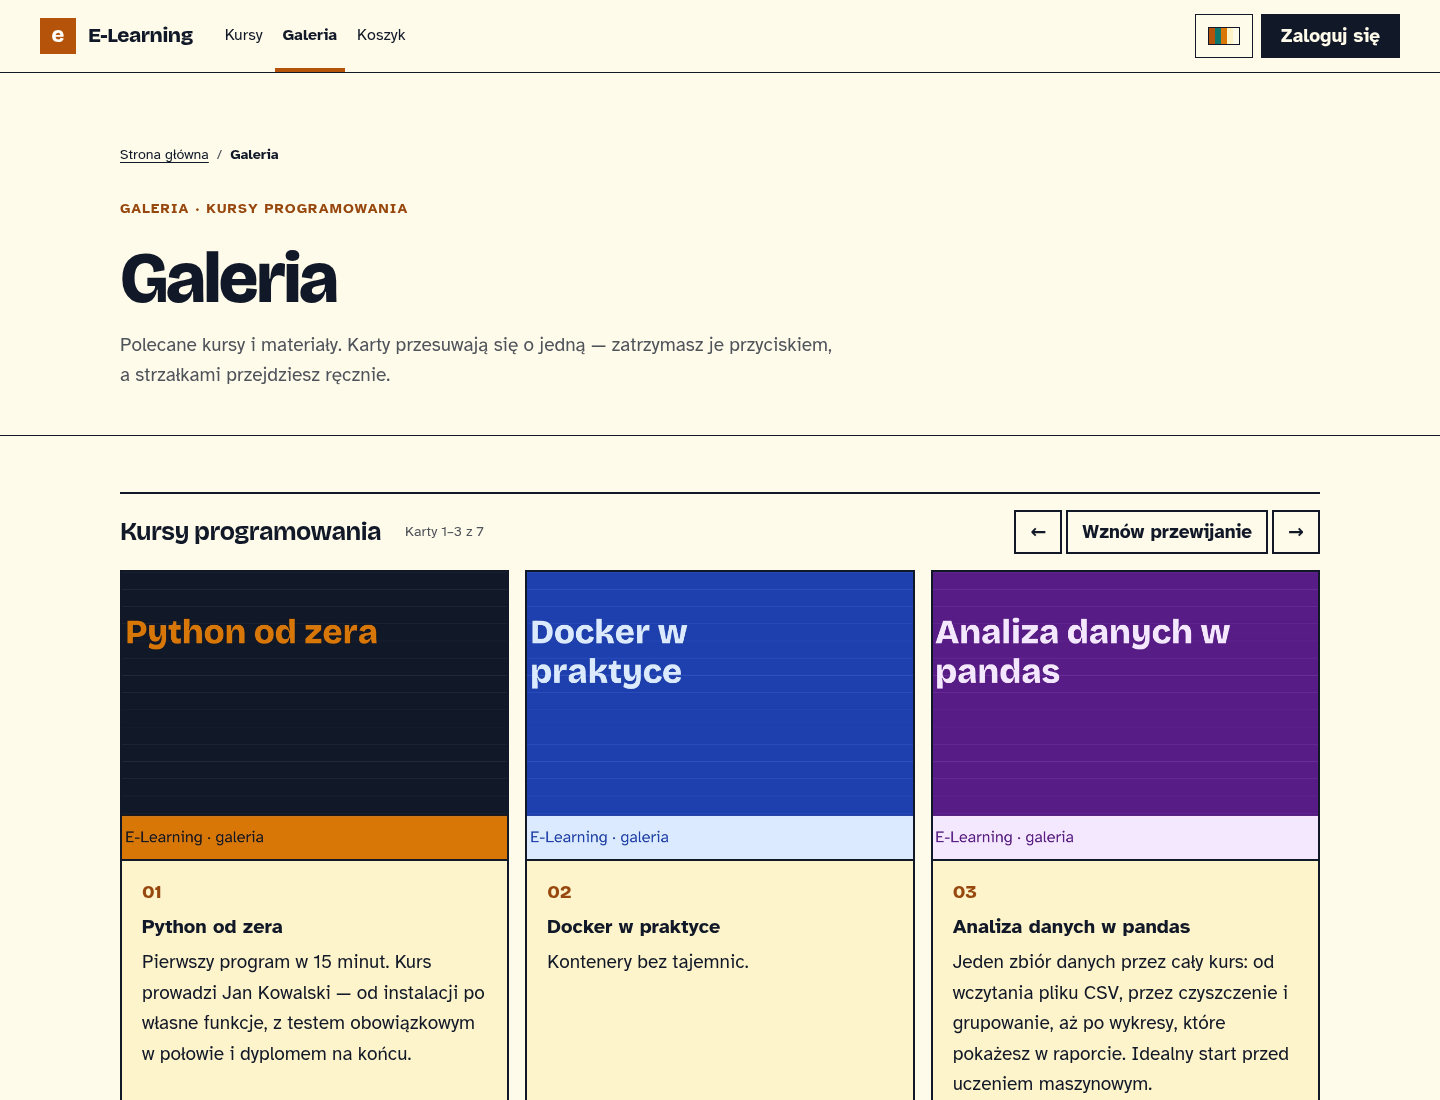
\includegraphics[width=0.94\linewidth,height=0.37\textheight,keepaspectratio]{img/slider.png}}
\caption{Publiczny slajder}\label{fig:ui-slider}
\end{figure}
Trzy karty na komputerze, pełne opisy, przyciski $\leftarrow$, pauza, $\rightarrow$ i~licznik ,,Karty 1--3 z~7''.




\chapter{Weryfikacja i~testy}\label{ch:testy}

\section{Strategia}

Weryfikację prowadzono na trzech poziomach:
\begin{enumerate}
  \item \textbf{testy automatyczne} (framework testowy Django) -- logika domenowa,
        uprawnienia, widoki, API, szablony (obecność etykiet i~atrybutów ARIA), dane demo;
  \item \textbf{kontrole statyczne projektu} -- \code{manage.py check} oraz
        \code{makemigrations --check}, wykonywane po każdej zmianie modelu;
  \item \textbf{weryfikacja ręczna w~przeglądarce} -- przejście ścieżek klawiaturą,
        pomiary układu na różnych szerokościach, scenariusze z~prawdziwymi usługami
        zewnętrznymi (Stripe w~trybie testowym, Bielik w~Ollamie).
\end{enumerate}

Usługi zewnętrzne są w~testach automatycznych zastępowane atrapami: klient Stripe jest
mockowany (a~webhook testowany z~\emph{prawdziwym} podpisem HMAC wyliczonym w~teście),
a~strumień Ollamy -- generatorem fragmentów. E-maile trafiają do \code{mail.outbox}.

\section{Testy automatyczne}

Ostatnie uruchomienie (5 listopada 2026, po dodaniu stylów uczenia się, ankiety, polecania kursów, panelu postępów, statystyk i~blokady logowania; PostgreSQL 16 w~Dockerze):

\begin{lstlisting}
$ python manage.py test
Ran 393 tests in 135.548s
OK
\end{lstlisting}

\begin{table}[H]
\centering\small
\caption{Zakres testów automatycznych}\label{tab:testy}
\begin{tabularx}{\linewidth}{@{}P{4.2cm}rL@{}}
\toprule
\hd{Plik} & \hd{Testy} & \hd{Zakres} \\
\midrule
\code{accounts/tests.py} & 36 & sesja i~logowanie, JWT (token, odświeżenie, \code{/api/me/}), wybór motywu (gość i~konto), OAuth2 i~łączenie z~istniejącym kontem, progi rang, sprawdzanie dostępności loginu \\
\code{catalog/tests.py} & 59 & modele kategorii i~kursów, wyszukiwarka i~sortowanie, zapisy, tworzenie i~edycja kursu, uprawnienia, XSS w~opisie, walidacja miniatur, powiadomienia o~zgłoszeniach \\
\code{catalog/test\_community.py} & 52 & drzewo komentarzy, dodawanie, edycja, usuwanie, akceptacja, głosy, kolejki moderacji, wątek zgłoszenia, zarządzanie kategoriami \\
\code{core/tests.py} i~pozostałe testy \code{core} & 52 & kontrast i~palety, motywy (także panel admina), strona główna, użyteczność szablonów (etykiety, \code{aria-current}, skip-link), odmiana liczebników, powiadomienia, menu konta \\
\code{core/test\_demo\_seed.py} & 4 & dane demo spełniają walidacje formularzy, \code{seed\_demo --reset} jest powtarzalny \\
\code{core/test\_image\_preview.py} & 6 & widżet podglądu zdjęcia, walidacja i~skalowanie awatara \\
\code{learning/tests.py} & 16 & kreator programu, dostęp do lekcji i~plików, upload zdjęć edytora, adresy filmów \\
\code{learning/test\_quizzes.py} & 28 & budowanie testów, blokady testem obowiązkowym, ocenianie automatyczne i~ręczne, ukończenie i~dyplom, tryb podglądu autora \\
\code{orders/tests.py} & 36 & koszyk i~kumulacja, scalanie koszyka gościa, zamówienie i~e-mail, Stripe i~webhook (podpis, kwota, idempotencja), obsługa statusów, kody, API koszyka JWT, formatowanie kwot \\
\code{chatbot/tests.py} & 23 & ochrona JWT, przebieg rozmowy i~strumień, blokada w~trakcie testu, strony historii, bezpieczne formatowanie odpowiedzi \\
\code{learning/test\_styles.py} & 34 & słownik stylów i~panel admina, wybór i~zmiana stylu, wersje lekcji (wybór, przełączanie, film, sanityzacja), uprawnienia autora, zapis stylu w~postępie i~podejściu, rekomendacja (brak danych, zmiana, utrzymanie, wybór), prompt asystenta \\
\code{learning/test\_survey\_recommend.py} & 17 & ankieta (10 pytań, walidacja, zachowanie odpowiedzi, ustawienie stylu), profil stylów, ranking i~uzasadnienie poleceń, katalog i~sortowanie, panel uczniów (uprawnienia, liczby, filtr), liczby ukończeń na stronie kursu \\
\code{accounts/test\_security.py} & 9 & blokada po 5 nieudanych logowaniach (login i~e-mail), zerowanie licznika, zmiana i~ustawienie hasła \\
\code{core/test\_stats.py} & 5 & statystyki tylko dla administratora, liczby zapisów, ukończeń i~procentów; walidacja kontrastu motywów \\
\code{gallery/tests.py} & 16 & upload ze skalowaniem, układy, zmiana kolejności (JSON i~$\uparrow\downarrow$), slajder publiczny, uprawnienia \\
\midrule
\textbf{Razem} & \textbf{393} & \\
\bottomrule
\end{tabularx}
\end{table}

Każdy widok zmieniający stan ma test odrzucenia metody GET (\emph{POST-only}) oraz test
uprawnień (np.\ uczeń nie zatwierdzi komentarza, nauczyciel nie oceni testu w~cudzej
kategorii, nikt nie oceni własnego podejścia, klient API bez tokenu dostaje 401).

\section{Weryfikacja ręczna}

\begin{table}[H]
\centering\small
\caption{Weryfikacja ręczna w~przeglądarce}
\begin{tabularx}{\linewidth}{@{}P{4.2cm}L@{}}
\toprule
\hd{Obszar} & \hd{Co sprawdzono} \\
\midrule
Klawiatura & przejście ścieżek gościa, ucznia, nauczyciela i~administratora wyłącznie klawiszami Tab, Shift+Tab, Enter, Spacja, strzałki i~Esc; powrót fokusu po zamknięciu paneli i~dialogów \\
Responsywność & nagłówek, slajder i~okno asystenta przy 320, 768, 1024, 1280, 1366, 1920 px -- bez poziomego przewijania \\
Slajder & pętla dla 4, 6 i~7 kart, 1/2/3 karty na widok, pauza, $\leftarrow\rightarrow$, brak automatu przy \code{prefers-reduced-motion} \\
Płatności & koszyk z~2 sztukami $\rightarrow$ Stripe Checkout (karta 4242, BLIK) $\rightarrow$ webhook 200 $\rightarrow$ ,,Opłacone'', wygenerowany kod, dwa e-maile \\
Asystent & Bielik-Minitron 7B (Q4\_K\_M) na GPU: odpowiedź ok. 5 s, strumień, Markdown, Esc i~fokus, blokada w~trakcie testu, komunikat przy wyłączonej Ollamie \\
Motywy & zmiana tokenów w~\code{main.css} oraz zmiana motywu w~panelu -- cała witryna, łącznie z~panelem administratora \\
\bottomrule
\end{tabularx}
\end{table}

\section{Automatyczny audyt dostępności}

Platformę sprawdzono narzędziami automatycznymi w~przeglądarce Chrome na danych demonstracyjnych,
z~zalogowanymi kontami wszystkich ról:

\begin{itemize}
  \item \textbf{axe-core 4.14} (reguły WCAG 2.0/2.1/2.2 A i~AA oraz \emph{best practices}):
        57 stron platformy przy szerokości 1366 px i~360 px, 16 stron panelu administracyjnego
        oraz 16 stron w~każdym z~motywów kolorystycznych -- \textbf{0 naruszeń}.
  \item \textbf{Lighthouse 13.6}: 14 kluczowych stron (strona główna, logowanie, katalog, kurs,
        lekcja, styl uczenia się, ankieta, zamówienie, panel uczniów, moderacja, statystyki,
        konfigurator slajdera, galeria, panel administracyjny) -- \textbf{dostępność 100/100,
        dobre praktyki 100/100}.
\end{itemize}

Audyt ujawnił i~pozwolił usunąć m.in.: przycisk powiadomień, którego nazwa nie zawierała widocznej
liczby (WCAG 2.5.3), linki w~tekście wyróżnione tylko kolorem (1.4.1), regiony o~powtarzającej się
nazwie, niedozwoloną rolę elementów listy w~slajderze, zbyt słaby kontrast czerwieni w~ciemnych
motywach, brak landmarku \code{main} i~etykiet pól w~tabelach panelu administracyjnego oraz brak
ikony strony. Dodatkowo panel administratora odrzuca teraz motyw kolorystyczny, który nie zapewnia
kontrastu 4,5:1 w~parach kolorów używanych przez arkusz (rozdz.~\ref{sec:theme-check}).

\section{Scenariusze testów użyteczności}

Projekt podlega testom użyteczności na platformie wybranej wspólnie przez studentów.
Przygotowano dla nich zestaw zadań odpowiadających najważniejszym ścieżkom; każde zadanie
uczestnik wykonuje najpierw myszą, a~następnie wyłącznie klawiaturą.

{\small
\begin{longtable}{@{}p{0.9cm}p{6.2cm}p{7.3cm}@{}}
\caption{Scenariusze testów użyteczności}\label{tab:scen}\\
\toprule
\hd{Nr} & \hd{Zadanie dla uczestnika} & \hd{Kryterium sukcesu} \\
\midrule
\endfirsthead
\toprule
\hd{Nr} & \hd{Zadanie dla uczestnika} & \hd{Kryterium sukcesu} \\
\midrule
\endhead
\bottomrule
\endlastfoot
TU-01 & Załóż konto i~zmień motyw na ciemny. & konto utworzone, motyw zachowany po wylogowaniu i~ponownym zalogowaniu \\
TU-02 & Znajdź bezpłatny kurs z~kategorii ,,Programowanie'' na poziomie podstawowym i~zapisz się. & użycie filtrów, zapis potwierdzony komunikatem \\
TU-03 & Dodaj płatny kurs dwa razy do koszyka i~opłać zamówienie kartą testową. & ilość 2 w~jednej pozycji, status ,,Opłacone'', kod dostępu widoczny w~zamówieniu \\
TU-04 & Przejdź pierwszą lekcję kursu Pythona i~rozwiąż test obowiązkowy. & lekcja oznaczona, wynik testu, odblokowanie kolejnych lekcji \\
TU-05 & Zapytaj asystenta o~fragment lekcji, a~potem spróbuj zapytać go w~trakcie testu. & odpowiedź z~kontekstem lekcji; w~trakcie testu -- odmowa \\
TU-06 & Dodaj komentarz z~oceną kursu, a~następnie odpowiedz na komentarz innej osoby. & komentarz oznaczony jako oczekujący, odpowiedź w~wątku \\
TU-07 & (nauczyciel) Zaakceptuj oczekujący komentarz i~oceń test otwarty. & komentarz opublikowany, uczeń dostaje powiadomienie \\
TU-08 & (nauczyciel) Utwórz kurs z~jedną sekcją i~lekcją i~wyślij go do publikacji. & przejście 3 kroków kreatora, kurs zatwierdzony w~kategorii nauczyciela \\
TU-09 & (administrator) Zmień kolejność kart slajdera bez użycia myszy. & przeniesienie przyciskami $\uparrow\downarrow$, nowa kolejność w~galerii \\
TU-10 & Odczytaj nowe powiadomienia i~oznacz wszystkie jako przeczytane. & licznik przy dzwonku wyzerowany \\
TU-11 & Wybierz styl uczenia się, otwórz lekcję z~wersjami i~przełącz się na inną wersję. & lekcja pokazuje wersję dla wybranego stylu, przełącznik dostępny z~klawiatury \\
TU-12 & Wypełnij ankietę stylu i~sprawdź polecane kursy w~katalogu. & wynik ankiety i~sekcja ,,Polecane dla Ciebie'' z~uzasadnieniem \\
TU-13 & (nauczyciel) Sprawdź, ilu uczniów ukończyło kurs i~kto ma najsłabsze wyniki testów. & odczyt z~panelu uczniów kursu bez pomocy \\
\end{longtable}
}

Dla każdego zadania notuje się: wykonanie (tak/nie), czas, liczbę błędów lub cofnięć oraz
uwagi uczestnika. Narzędzia automatyczne (Lighthouse, axe, WAVE) służą jako uzupełnienie
-- wykrywają brakujące etykiety, kontrast i~błędy struktury, ale nie zastępują przejścia
ścieżki klawiaturą.

\chapter{Przebieg realizacji}

Projekt zrealizowano samodzielnie w~okresie od 7 października do 4 listopada 2026 roku.
Prace podzielono na sześć etapów. Etapy częściowo się nakładały: od chwili, gdy gotowy był
model danych i~system stylów, moduły funkcjonalne rozwijano równolegle, a~każdy kończył się
kompletem testów, danymi demonstracyjnymi i~wpisem w~dzienniku stanu projektu. Zasada
,,moduł jest skończony, gdy ma URL, szablon, test i~dane demo'' pozwoliła uniknąć
odkładania integracji na koniec.

\section{Diagram Gantta}

\begin{figure}[H]
\centering
\resizebox{\linewidth}{!}{%
\begin{ganttchart}[
  time slot format=isodate,
  x unit=0.48cm, y unit chart=0.55cm, y unit title=0.6cm,
  vgrid={*6{draw=none},*1{ink!25,dotted}},
  hgrid style/.style={draw=ink!10},
  title/.style={draw=ink!40,fill=paperdark},
  title label font=\sffamily\scriptsize\bfseries,
  bar/.style={draw=ink,fill=brand!70},
  bar height=0.55,
  group/.style={draw=ink,fill=ink},
  group height=0.25, group peaks height=0.15, group peaks width=0.25,
  bar label font=\sffamily\scriptsize,
  group label font=\sffamily\scriptsize\bfseries,
  milestone/.style={draw=ink,fill=brandteal},
  milestone label font=\sffamily\scriptsize\bfseries,
  today=2026-11-05, today rule/.style={draw=brand,dashed,thick},
  today label=dziś, today label font=\sffamily\scriptsize\color{brand},
]{2026-10-07}{2026-11-05}
  \gantttitle{Październik 2026}{25}\gantttitle{Listopad 2026}{5} \\
  \gantttitle{7.10}{5}\gantttitle{12.10}{7}\gantttitle{19.10}{7}\gantttitle{26.10}{7}\gantttitle{2.11}{4} \\
  \ganttgroup{I. Analiza i~projekt}{2026-10-07}{2026-10-14} \\
  \ganttbar{1. Analiza wymagań, wybór technologii}{2026-10-07}{2026-10-09} \\
  \ganttbar{2. Model danych, podział na moduły}{2026-10-09}{2026-10-14} \\
  \ganttbar{3. Makiety i~język wizualny}{2026-10-10}{2026-10-14} \\
  \ganttgroup{II. Fundament}{2026-10-13}{2026-10-24} \\
  \ganttbar{4. Django, Docker Compose, PostgreSQL, Redis}{2026-10-13}{2026-10-15} \\
  \ganttbar{5. Konta, role, logowanie, JWT}{2026-10-15}{2026-10-20} \\
  \ganttbar{6. OAuth2: Discord, GitLab, Bitbucket}{2026-10-19}{2026-10-22} \\
  \ganttbar{7. System stylów i~motywy kolorów}{2026-10-16}{2026-10-24} \\
  \ganttgroup{III. Katalog i~społeczność}{2026-10-21}{2026-10-30} \\
  \ganttbar{8. Kategorie MPTT, katalog, okruszki}{2026-10-21}{2026-10-24} \\
  \ganttbar{9. Kreator kursu, zgłoszenia, moderacja}{2026-10-23}{2026-10-28} \\
  \ganttbar{10. Komentarze, głosy, rangi, powiadomienia}{2026-10-26}{2026-10-30} \\
  \ganttgroup{IV. Nauka i~galeria}{2026-10-24}{2026-10-30} \\
  \ganttbar{11. Program kursu: sekcje, lekcje, postęp}{2026-10-24}{2026-10-28} \\
  \ganttbar{12. Testy ABC/otwarte, ocenianie, dyplomy}{2026-10-27}{2026-10-30} \\
  \ganttbar{13. Galeria: upload, konfigurator DnD, slajder}{2026-10-27}{2026-10-30} \\
  \ganttbar{14. Redesign wszystkich widoków}{2026-10-28}{2026-10-30} \\
  \ganttgroup{V. Sklep, asystent AI, style uczenia się}{2026-10-29}{2026-11-04} \\
  \ganttbar{15. Koszyk, zamówienia, Stripe, webhook}{2026-10-29}{2026-11-01} \\
  \ganttbar{16. Asystent Bielik: Ollama, strumień, JWT}{2026-10-30}{2026-11-01} \\
  \ganttbar{17. Style uczenia się: wersje lekcji, analiza}{2026-11-01}{2026-11-03} \\
  \ganttbar{18. Ankieta, polecanie kursów, postępy, statystyki}{2026-11-02}{2026-11-04} \\
  \ganttgroup{VI. Weryfikacja i~oddanie}{2026-10-28}{2026-11-04} \\
  \ganttbar{19. Dane demonstracyjne (seed)}{2026-10-28}{2026-11-02} \\
  \ganttbar{20. Testy, przegląd dostępności, poprawki}{2026-11-01}{2026-11-03} \\
  \ganttbar{21. Dokumentacja i~instrukcje}{2026-11-02}{2026-11-04} \\
  \ganttmilestone{Zakończenie prac}{2026-11-04}
\end{ganttchart}}
\caption{Diagram Gantta -- harmonogram realizacji projektu}\label{fig:gantt}
\end{figure}

\section{Zestawienie zadań}

\begin{table}[H]
\centering\small
\caption{Zadania projektu i~terminy}\label{tab:zadania}
\begin{tabularx}{\linewidth}{@{}rLccr@{}}
\toprule
\hd{Nr} & \hd{Zadanie} & \hd{Początek} & \hd{Koniec} & \hd{Dni} \\
\midrule
1 & Analiza wymagań prowadzącego, wybór technologii & 07.10 & 09.10 & 3 \\
2 & Model danych, podział na aplikacje, decyzje projektowe & 09.10 & 14.10 & 6 \\
3 & Makiety interfejsu i~język wizualny ,,plan zajęć'' & 10.10 & 14.10 & 5 \\
4 & Szkielet Django, Docker Compose, PostgreSQL, Redis, \code{.env} & 13.10 & 15.10 & 3 \\
5 & \code{CustomUser}, role, logowanie i~rejestracja, JWT & 15.10 & 20.10 & 6 \\
6 & OAuth2 (Discord, GitLab, Bitbucket), łączenie kont & 19.10 & 22.10 & 4 \\
7 & \code{main.css}, 5 tokenów, \code{ColorTheme}, kontrast, przełącznik & 16.10 & 24.10 & 9 \\
8 & Kategorie MPTT, katalog z~filtrami, okruszki & 21.10 & 24.10 & 4 \\
9 & Kreator kursu, zgłoszenia z~wątkiem, kolejki moderacji & 23.10 & 28.10 & 6 \\
10 & Komentarze w~wątkach, głosy, rangi, centrum powiadomień & 26.10 & 30.10 & 5 \\
11 & Sekcje, lekcje, załączniki, filmy, postęp & 24.10 & 28.10 & 5 \\
12 & Testy ABC/wielokrotne/otwarte, ocena ręczna, dyplomy PDF & 27.10 & 30.10 & 4 \\
13 & Galeria: skalowanie, układy, przeciąganie, slajder & 27.10 & 30.10 & 4 \\
14 & Redesign wszystkich stron (w~tym allauth i~panel admina) & 28.10 & 30.10 & 3 \\
15 & Koszyk, zamówienia, e-mail, Stripe + webhook, kody & 29.10 & 01.11 & 4 \\
16 & Asystent Bielik: widżet, API strumieniowe, historia & 30.10 & 01.11 & 3 \\
17 & Style uczenia się: słownik stylów, wersje lekcji, analiza i~rekomendacja & 01.11 & 03.11 & 3 \\
18 & Ankieta stylu, polecanie kursów, panel postępów, statystyki, blokada logowania & 02.11 & 04.11 & 3 \\
19 & Dane demonstracyjne (\code{seed\_demo}) & 28.10 & 02.11 & 6 \\
20 & Testy automatyczne, przegląd klawiatury i~RWD, poprawki & 01.11 & 03.11 & 3 \\
21 & Dokumentacja, instrukcje uruchomienia & 02.11 & 04.11 & 3 \\
\bottomrule
\end{tabularx}
\end{table}

\section{Opis etapów}

\subsection*{Etap I -- analiza i~projekt (07--14.10)}
Rozpisano wymagania prowadzącego na moduły i~punktację, zdecydowano o~monolicie Django
z~renderowaniem po stronie serwera (prostsze spełnienie wymagań dostępności niż w~aplikacji
SPA) i~o~lokalnym modelu językowym. Zaprojektowano model danych z~rozstrzygnięciem
niejasności (np.\ moderator = nauczyciel, test po lekcji lub na końcu, kody dostępu dla
kolejnych sztuk kursu). Przygotowano makiety i~zasady języka wizualnego, w~tym decyzję
o~pięciu kolorach bazowych.

\subsection*{Etap II -- fundament (13--24.10)}
Powstało środowisko Docker Compose, rozszerzony model użytkownika z~rolami, logowanie,
rejestracja z~zachowaniem danych po błędzie, tokeny JWT i~logowanie przez trzy portale
OAuth2 z~pobieraniem profilu. Równolegle zbudowano system stylów oparty na tokenach,
moduł kontrastu WCAG, motywy w~bazie i~przełącznik motywu dostępny z~klawiatury.

\subsection*{Etap III -- katalog i~społeczność (21--30.10)}
Drzewo kategorii z~przydziałem moderatorów, katalog z~filtrami, trzyetapowy kreator
kursu ze szkicem, zgłoszenia z~trwałym wątkiem, kolejki moderacji, komentarze w~wątkach
z~akceptacją i~edycją, głosy z~przeliczaniem reputacji oraz centrum powiadomień.

\subsection*{Etap IV -- nauka i~galeria (24--30.10)}
Program kursu z~edytorem lekcji, testy wszystkich typów z~blokadami i~oceną ręczną,
dyplomy PDF oraz trzy widoki galerii z~przeciąganiem i~zapętlonym slajderem. Na koniec etapu przeprowadzono redesign wszystkich widoków
w~jednolitym stylu.

\subsection*{Etap V -- sklep, asystent AI i~style uczenia się (29.10--04.11)}
Koszyk z~kumulacją i~scalaniem koszyka gościa, zamówienie z~adresem z~profilu,
potwierdzenia e-mail, integracja Stripe Checkout z~webhookiem i~kodami dostępu (sprawdzona
na prawdziwym koncie testowym). Asystent Bielik z~oknem czatu, strumieniowaniem,
kontekstem lekcji i~wyniku testu, blokadą w~trakcie testu i~historią rozmów (sprawdzony
z~modelem 7B). Na koniec etapu dodano style uczenia się: słownik stylów zarządzany przez
administratora, wersje lekcji dla stylów, wybór stylu przez ucznia oraz analizę wyników testów
z~rekomendacją stylu, a~następnie ankietę diagnostyczną, polecanie kursów dopasowanych do profilu
stylów ucznia, panel postępów uczniów dla nauczyciela, statystyki platformy oraz zmianę hasła
i~czasową blokadę logowania.

\subsection*{Etap VI -- weryfikacja i~oddanie (28.10--04.11)}
Komplet danych demonstracyjnych odtwarzanych jednym poleceniem, uzupełnienie testów
automatycznych do 393, automatyczny audyt dostępności (axe, Lighthouse), przegląd klawiatury i~responsywności, instrukcje uruchomienia
(Windows, Stripe, asystent) oraz niniejsza dokumentacja.

\chapter{Instalacja i~uruchomienie}

\section{Wymagania środowiskowe}

\begin{itemize}
  \item Docker Engine z~Docker Compose v2 (Linux) albo Docker Desktop z~WSL 2 (Windows,
        szczegółowa instrukcja: \code{docs/uruchomienie-windows.md}), ok. 2 GB miejsca na
        obrazy i~dane;
  \item opcjonalnie dla asystenta AI: ok. 5 GB na model Bielik 7B oraz 8 GB RAM (zalecana
        karta graficzna -- wtedy Ollamę najlepiej uruchomić bezpośrednio na komputerze);
  \item opcjonalnie: konto testowe Stripe (klucze \code{sk\_test\_}/\code{pk\_test\_}) oraz
        aplikacje OAuth2 w~Discordzie, GitLabie i~Bitbuckecie.
\end{itemize}

Bez kluczy Stripe, OAuth2 i~bez Ollamy platforma uruchamia się w~pełni -- odpowiednie moduły
pokazują wtedy czytelny komunikat zamiast błędu.

\section{Pierwsze uruchomienie}

\begin{lstlisting}
cp .env.example .env                 # Windows: Copy-Item .env.example .env
# w .env ustaw DJANGO_SECRET_KEY na długi losowy ciąg znaków
docker compose up --build -d         # db + redis + web; web wykonuje migracje przy starcie
docker compose exec -T web python scripts/seed_data.py --reset   # dane demonstracyjne
# platforma: http://localhost:8000     panel administracyjny: http://localhost:8000/admin/
\end{lstlisting}

\subsection*{Najważniejsze zmienne \code{.env}}

\begin{table}[H]
\centering\small
\caption{Konfiguracja środowiska}
\begin{tabularx}{\linewidth}{@{}P{5.0cm}L@{}}
\toprule
\hd{Zmienna} & \hd{Znaczenie} \\
\midrule
\code{DJANGO\_SECRET\_KEY}, \code{DJANGO\_DEBUG}, \code{DJANGO\_ALLOWED\_HOSTS} & podstawowa konfiguracja Django \\
\code{POSTGRES\_*}, \code{DB\_HOST\_PORT} & baza danych; port na hoście (domyślnie 5433) \\
\code{REDIS\_URL}, \code{REDIS\_HOST\_PORT} & Redis; port na hoście (domyślnie 6380) \\
\code{EMAIL\_BACKEND}, \code{DEFAULT\_FROM\_EMAIL}, \code{SITE\_URL} & wysyłka e-maili (domyślnie do konsoli), adres w~linkach \\
\code{STRIPE\_SECRET\_KEY}, \code{STRIPE\_PUBLISHABLE\_KEY}, \code{STRIPE\_WEBHOOK\_SECRET} & płatności testowe; sekret webhooka może zostać pusty przy usłudze \code{stripe-cli} \\
\code{OLLAMA\_BASE\_URL}, \code{OLLAMA\_MODEL}, \code{OLLAMA\_TIMEOUT} & adres Ollamy (\code{http://ollama:11434} lub \code{http://host.docker.internal:11434}), model, limit czasu \\
\code{CHATBOT\_QUIZ\_LOCK\_MINUTES} & czas blokady asystenta po otwarciu testu \\
\code{DISCORD\_*}, \code{GITLAB\_*}, \code{BITBUCKET\_*} & identyfikatory i~sekrety aplikacji OAuth2 \\
\bottomrule
\end{tabularx}
\end{table}

\section{Moduły opcjonalne}

\paragraph{Asystent AI} (szczegóły: \code{docs/asystent-bielik.md}):
\begin{lstlisting}
docker compose --profile ai up -d ollama
docker compose exec ollama ollama pull hf.co/speakleash/Bielik-Minitron-7B-v3.0-Instruct-GGUF:Q4_K_M
\end{lstlisting}
Przy Ollamie zainstalowanej na komputerze wystarczy \code{ollama pull} tego modelu
i~ustawienie \code{OLLAMA\_BASE\_URL=http://host.docker.internal:11434}.

\paragraph{Płatności Stripe} (szczegóły: \code{docs/platnosci-stripe.md}): wpisać klucze
testowe w~\code{.env} i~uruchomić \code{docker compose --profile stripe up -d}. Usługa
\code{stripe-cli} nasłuchuje zdarzeń, przekazuje je na \code{/orders/webhook/stripe/}
i~sama zapisuje sekret \code{whsec\_} w~\code{.stripe/webhook\_secret}. Karta testowa:
\code{4242 4242 4242 4242}, dowolna przyszła data i~CVC.

\paragraph{Logowanie przez portale}: w~każdym portalu utworzyć aplikację OAuth2 z~adresem
zwrotnym \code{http://localhost:8000/accounts/social/<portal>/login/callback/}
(\code{discord}, \code{gitlab}, \code{bitbucket\_oauth2}) i~wpisać identyfikator oraz
sekret do \code{.env}.

\section{Dane demonstracyjne i~konta testowe}

Polecenie \code{seed\_demo} (oraz jego nakładka \code{scripts/seed\_data.py}) tworzy komplet
danych pokazujących każdy moduł: drzewo 11 kategorii, 10 opublikowanych kursów
z~okładkami, sekcjami, lekcjami (kod, tabele, zdjęcia, pliki, filmy) i~testami wszystkich
typów, zapisy z~postępem, podejścia zaliczone, niezaliczone i~czekające na ocenę, dyplomy,
komentarze w~wątkach z~głosami, zgłoszenia kursów z~wątkiem, zamówienia we wszystkich
statusach z~kodem dostępu, zdjęcia galerii z~trzema układami slajdera, rozmowy z~asystentem,
powiadomienia, motywy kolorystyczne oraz style uczenia się: style wybrane przez pięciu
uczniów, osiem wersji lekcji w~kursie Pythona i~historię wyników, dzięki której system
poleca uczniowi \code{student2} zmianę stylu, style polecane przez autorów w~9 kursach oraz pięć
wypełnionych ankiet. Bez flagi \code{--reset} polecenie dopisuje tylko
brakujące dane.

\begin{table}[H]
\centering\small
\caption{Konta testowe}\label{tab:konta}
\begin{tabularx}{\linewidth}{@{}P{3.4cm}P{2.6cm}P{2.0cm}L@{}}
\toprule
\hd{Rola} & \hd{Login} & \hd{Hasło} & \hd{Co warto pokazać} \\
\midrule
Administrator & \code{admin} & \code{admin123!} & Moderacja, kategorie, galeria i~układy slajdera, motywy, style uczenia się, panel \code{/admin/} \\
Nauczyciel (moderator) & \code{instructor} & \code{test123!} & tworzenie kursu, wersje lekcji dla stylów, kolejki akceptacji, ocenianie testów, zamówienia \\
Nauczyciele & \code{m.wisniewska}, \code{p.zielinski}, \code{k.lewandowska} & \code{test123!} & moderatorzy innych kategorii \\
Uczeń & \code{student1} & \code{test123!} & moje kursy, lekcje w~wersji ,,Wzrokowiec'', testy, dyplom, asystent \\
Uczeń & \code{student2} & \code{test123!} & rekomendacja stylu ,,Praktyk'', koszyk z~kumulacją, zamówienia \\
Uczeń bez wybranego stylu & \code{kuba.dabrowski} & \code{test123!} & wynik ankiety (Praktyk 80\%) i~polecane kursy tylko z~ankiety \\
Pozostali uczniowie & np.\ \code{ola.krawczyk} & \code{test123!} & komentarze, głosy, różne motywy \\
\bottomrule
\end{tabularx}
\end{table}

\section{Codzienne polecenia}

\begin{table}[H]
\centering\small
\caption{Polecenia administracyjne}
\begin{tabularx}{\linewidth}{@{}P{6.6cm}L@{}}
\toprule
\hd{Polecenie} & \hd{Działanie} \\
\midrule
\code{docker compose up -d} / \code{stop} & uruchomienie / zatrzymanie (dane zostają) \\
\code{docker compose logs -f web} & podgląd logów aplikacji (także e-maili w~trybie deweloperskim) \\
\code{docker compose exec web python manage.py test} & testy automatyczne \\
\code{docker compose exec web python manage.py check} & kontrola konfiguracji \\
\code{... manage.py makemigrations --check --dry-run} & kontrola, czy modele mają migracje \\
\code{... manage.py createsuperuser} & własne konto administratora \\
\code{... scripts/seed\_data.py --reset} & odtworzenie danych demo od zera \\
\code{docker compose down -v} & usunięcie kontenerów wraz z~bazą i~plikami \\
\bottomrule
\end{tabularx}
\end{table}

Praca bez Dockera dla aplikacji: wirtualne środowisko \code{.venv} z~\code{requirements.txt},
baza i~Redis z~Compose, a~w~poleceniach \code{POSTGRES\_HOST=localhost POSTGRES\_PORT=5433}.

\section{Rozwiązywanie problemów}

\begin{table}[H]
\centering\small
\caption{Typowe problemy}
\begin{tabularx}{\linewidth}{@{}P{5.4cm}L@{}}
\toprule
\hd{Objaw} & \hd{Rozwiązanie} \\
\midrule
\code{port is already allocated} (8000, 5433, 6380) & zmienić \code{DB\_HOST\_PORT}/\code{REDIS\_HOST\_PORT} w~\code{.env} lub zwolnić port \\
\code{env file .env not found} & skopiować \code{.env.example} do \code{.env} (uwaga na nazwę \code{.env.txt} w~Windows) \\
Strona nie odpowiada zaraz po starcie & pierwszy start wykonuje migracje -- poczekać na \code{Starting development server} w~logach \\
Asystent: ,,serwer modelu nie odpowiada'' & uruchomić Ollamę (profil \code{ai} lub na hoście) i~sprawdzić \code{OLLAMA\_BASE\_URL} \\
Asystent: ,,model nie jest pobrany'' & \code{ollama pull} z~nazwą z~\code{OLLAMA\_MODEL} \\
Zamówienie zostaje ,,Oczekuje na płatność'' & uruchomić \code{stripe-cli}; ewentualnie odświeżyć stronę zamówienia -- system sam sprawdzi stan w~Stripe \\
Logowanie przez portal: \code{redirect\_uri mismatch} & adres zwrotny w~portalu musi dokładnie odpowiadać podanemu wyżej \\
\bottomrule
\end{tabularx}
\end{table}

\section{Uwagi do wdrożenia produkcyjnego}

Konfiguracja w~repozytorium jest przeznaczona do pracy deweloperskiej i~prezentacji. Przy
wdrożeniu publicznym należy: ustawić \code{DJANGO\_DEBUG=False} i~właściwe
\code{ALLOWED\_HOSTS}, uruchomić aplikację przez \code{gunicorn} (jest w~zależnościach) za
serwerem WWW obsługującym pliki statyczne i~media (także żądania zakresowe dla filmów),
włączyć HTTPS z~bezpiecznymi ciasteczkami, HSTS i~\code{CSRF\_TRUSTED\_ORIGINS}, ograniczyć
CORS, skonfigurować prawdziwy serwer SMTP oraz produkcyjny webhook Stripe z~własnym
sekretem.

\chapter{Podsumowanie}

\section{Stan realizacji}

Zrealizowano wszystkie moduły przewidziane w~specyfikacji wraz z~rozszerzeniami
punktowanymi oraz szeregiem usprawnień wykraczających poza nią. Zestawienie z~wymaganiami
prowadzącego przedstawia tabela~\ref{tab:realizacja}.

\begin{table}[H]
\centering\small
\caption{Realizacja wymagań specyfikacji}\label{tab:realizacja}
\begin{tabularx}{\linewidth}{@{}P{3.8cm}L@{}}
\toprule
\hd{Moduł} & \hd{Zrealizowane elementy} \\
\midrule
UI/UX, WCAG, usability & autorski system stylów bez bibliotek, pełna obsługa klawiaturą, widoczny fokus, etykiety, Esc w~każdym panelu, RWD 320--1920 px, brak \code{alert/confirm/prompt} \\
Konta i~OAuth2 & sesja + JWT, zmiana hasła, blokada po 5 nieudanych logowaniach, trzy portale spoza Google/GitHub z~pobraniem profilu i~awatara, split-screen logowania, zachowanie danych po błędzie \\
Galeria i~slajder & trzy widoki, skalowanie Pillow, wiele układów, DnD z~\code{fetch} i~alternatywą klawiaturową, zapętlony slajder 1/2/3 \\
Katalog i~moderacja & drzewo MPTT z~okruszkami, CKEditor + bleach, zgłoszenia z~trwałym wątkiem, komentarze z~akceptacją, oceny i~rangi, centrum powiadomień, paginacja wszystkich list \\
E-commerce & kumulacja w~koszyku, adres z~profilu z~zapisem, e-mail, statusy, Stripe sandbox + webhook $\rightarrow$ ,,Opłacone'' $\rightarrow$ dostęp do kursu \\
E-learning i~AI & lekcje, pytania z~tekstem, zdjęciem i~filmem, ABC liczone automatycznie, pytania otwarte ze zdjęciem i~oceną ręczną z~powiadomieniem, Bielik przez Ollamę z~API JWT \\
Style uczenia się (rozszerzenie) & 4 style VARK + style dodawane przez admina, ankieta diagnostyczna, wybór i~zmiana stylu przez ucznia, wersje lekcji dla stylów, analiza wyników i~rekomendacja stylu, polecanie kursów dopasowanych do profilu \\
Postępy i~statystyki & panel uczniów kursu dla nauczyciela, statystyki platformy dla administratora, liczba osób, które kurs zaczęły i~ukończyły, z~procentem ukończenia \\
Motywy & 5 tokenów, odcienie przez \code{color-mix}/\code{hsl(from)}, edycja w~panelu z~próbnikami, motywy w~profilu na każdym urządzeniu \\
Dokumentacja, uruchomienie & Docker Compose, \code{requirements.txt}, skrypt danych testowych, instrukcje, niniejszy dokument, 393 testy automatyczne, audyt axe i~Lighthouse bez błędów (dostępność 100/100) \\
\bottomrule
\end{tabularx}
\end{table}

\section{Wnioski}

\begin{itemize}
  \item \textbf{Renderowanie po stronie serwera ułatwiło dostępność.} Formularze HTML,
        natywne \code{details} i~\code{dialog} oraz zasada ,,najpierw działa bez JS'' dały
        obsługę klawiatury i~czytników ekranu niemal za darmo; JavaScript dodaje jedynie
        wygodę.
  \item \textbf{Kolory wyliczane zamiast wpisywanych.} Obliczanie koloru tekstu
        z~kontrastu sprawiło, że administrator nie może utworzyć nieczytelnego motywu,
        a~pięć tokenów wystarczyło do pokolorowania całej platformy i~panelu administracyjnego.
  \item \textbf{Usługi zewnętrzne jako elementy opcjonalne.} Platforma działa bez
        płatności, portali i~modelu językowego, co upraszcza prezentację i~testy, a~awaria
        jednej usługi nie wyłącza pozostałych funkcji.
  \item \textbf{Moduły kończone ,,pionowo''.} Każda funkcja powstawała od modelu, przez
        widok i~szablon, po test i~dane demo -- dzięki temu w~każdym momencie projekt nadawał
        się do pokazania.
\end{itemize}

\section{Kierunki rozwoju}

\begin{itemize}
  \item Kolejka zadań (np.\ Celery na istniejącym Redisie) dla e-maili i~generowania
        dyplomów, aby nie wydłużały odpowiedzi.
  \item Serwowanie filmów przez serwer WWW z~obsługą żądań zakresowych i~ewentualna
        transkodacja.
  \item Raporty dla nauczyciela: statystyki pytań (najczęstsze błędne odpowiedzi),
        eksport wyników do CSV.
  \item Wyszukiwanie pełnotekstowe PostgreSQL w~katalogu i~treści lekcji.
  \item Indeksowanie treści kursu (RAG) dla asystenta, aby odpowiadał na podstawie całego
        kursu, a~nie tylko bieżącej lekcji.
  \item Faktury i~produkcyjne metody płatności po wyjściu z~trybu testowego.
\end{itemize}


\end{document}
